\documentclass[twoside]{report} % double side

% Packages ---------------------------------------------------------------
% the package 'umlaute' calls only the package 'inputenc' creating a warning (UJG, 04.05.2011)
%
% \usepackage[ansi]{umlaute} % --- Unterstuetzen von deutschen Umlauten
\usepackage[latin1]{inputenc}   %--->for ubuntu linux
% \usepackage[utf8]{inputenc}   %--->for ubuntu linux
%for latex
\usepackage{etex} % for allocating registers when a large number of packages is used
\usepackage[dvips]{graphicx}
%for pdflatex
%\usepackage[pdftex]{graphicx}
%\usepackage{epstopdf}
\usepackage{float,color,latexsym, epic,eepic,rotating}
\usepackage{fheading}           % Seitenkopf gestalten
\usepackage{amssymb, amsmath}
\usepackage{epsfig}
\usepackage{bm}
\usepackage[usenames,dvipsnames]{pstricks}
% Who added this, please comment
\makeatletter
\renewcommand\thefigure{\thesection.\arabic{figure}}
\makeatother
\usepackage[version=3]{mhchem}
\usepackage{booktabs}
%\usepackage{units}
\newcommand{\unit}[1]{\ensuremath{\, \mathrm{#1}}}
\usepackage{subfigure}
\usepackage{caption}
\captionsetup{format=hang,justification=raggedright,justification=justified}
\usepackage{color}
\usepackage[hyperref, dvips, colorlinks, linkcolor=black,citecolor=black, urlcolor=black]{hyperref}
\usepackage{ltablex}  %to generate automatic line breaks in table ( compination of landscape and tabularx)
\usepackage{longtable}
\usepackage{lscape}% to get table in landscape format
\usepackage{paralist}
\usepackage{arydshln}
\usepackage{pst-grad} % For gradients
\usepackage{pst-plot} % For axes
\usepackage{fancybox} % shadow box
\usepackage{multirow}
\usepackage{tikz} % For some figures DDF
\usetikzlibrary{patterns} % For some figures DDF

% Layout -----------------------------------------------------------------
\setlength{\parindent}{0pt}
\setlength{\parskip}{5pt plus 2pt minus 1pt}
%\renewcommand{\arraystretch}{1.2}
\pagestyle{fancy}
\lhead[\fancyplain{}{\footnotesize\textsf\thepage}]%
      {\fancyplain{}{\footnotesize\textsf\rightmark}}
\rhead[\fancyplain{}{\footnotesize\textsf\leftmark}]%
      {\fancyplain{}{\footnotesize\textsf\thepage}}
\cfoot{}
\setcounter{tocdepth}{1}
%Zaehler
%\setcounter{page}{65}
%\setcounter{section}{8}
%\setcounter{equation}{213}
%\setcounter{figure}{24}
%\setcounter{table}{9}
%\pagenumbering{arabic} \setcounter{page}{1}
% Trennmuster fuer Ausnahmefaelle
\hyphenation{me-cha-nik}
\hyphenation{pro-per-ties}
\makeindex

% Makros -----------------------------------------------------------------
% % general
\newcommand{\D}{\displaystyle}
%%\newcommand{\Vec}[1]{{\bf \bar{#1} }}
\newcommand{\Boldmath}[1]{\mbox{\boldmath ${#1}$ \unboldmath}}
%%\newcommand{\boldsymbol}[1]{\mbox{\boldmath ${#1}$ \unboldmath}}
% geometry
\def \VolSol {V}
\def \AreaSol {A}
\def \Domain {\Omega}
% fluid flow
\def \Phase {\gamma}
\def \VolumetricFraction {\epsilon}
\newcommand{\p}{\partial}
\newcommand{\PiezoHead}{p/g\rho+z}
\def \Viscosity {\mu}
\def \Pressure {p}
\def \Perm {k}
\def \Source {Q}
\def \Porosity {n}%{\theta^f}
\def \DensSolid {\rho^s}
\def \DensFluid {\rho^f}
\def \Density {\rho}
\def \DarcyVelo {q}
\def \DarcyVeloVector {\mathbf\DarcyVelo}
\def \Gravity {g}
\def \GravityVector {\mathbf{g}}
\def \Stor {S}
\def \FluidCompressibility {\beta_p}
\def \ThermalExpansionCoefficient {\beta_T}
%
\def \PermRelP {k_{\mbox{\footnotesize rel}}}
\def \PermTensorRelComp {k_{\alpha\beta}^0}
\def \PermTensor {\mathbf{k}}
\def \FluidMassSourceP {Q_\rho^p}
\def \Saturation {S}
\def \MoistureContent {\theta}
\def \CapillaryPressure {\Pressure_{\mbox{\footnotesize c}}}
\def \PermRelS {k_{\mbox{\footnotesize rel}}}
\def \SaturationEff {\Saturation_{\mbox{\footnotesize eff}}}
\def \SaturationMax {\Saturation_{\mbox{\footnotesize max}}}
\def \SaturationRes {\Saturation_r}
\def \GasVelocityVector {{\mathbf{v}}^{g}}
\def \WaterVelocityVector {{\mathbf{v}}^{w}}
\def \VelocityVector {{\mathbf{v}}}
% deformation
\newcommand{\U}{u}
\newcommand{\Stress}{\mbox{\boldmath $\sigma$}}
\newcommand{\Shear}{\mbox{\boldmath $\tau$ \unboldmath}}
\def \Treps {\varepsilon}
% mass transport
\def \Conc {C}
\def \Solubility {C_s}
\def \VeloDisso {Rd}
\def \Diffusion {D}
% heat transport
\def \TLatentB {T_{l1}}
\def \TLatentE {T_{l2}}
\def \Temperature {T}
\def \HeatCapacity {c}
\def \HeatConductivity {\lambda}
\def \LatentHeat {L_0}
\def \Enthalpy {H}
% numerics
\newcommand{\Ne}{\frac{\alpha\Delta t}{\Delta x^2}}
\newcommand{\WF}{\omega}
\newcommand{\IF}{\phi}
\newcommand{\SF}{N}
\newcommand{\SFV}{{\mathbf\SF}}
\def \SFVPressure {\SFV_p}
\newcommand{\JacOneD}{[J_{1D}]}
\newcommand{\JacTwoD}{[J_{2D}]}
\newcommand{\JacInvOneD}{[J_{1D}^{-1}]}
\newcommand{\JacInvTwoD}{[J_{2D}^{-1}]}
\newcommand{\SFGradOneD}{[\nabla_r \SF]}
\newcommand{\SFGradTwoD}{[\nabla_{rs} \SF]}
\newcommand{\WFV}{\mbox{\boldmath $\omega$ \unboldmath}}
\newcommand{\IFV}{\mbox{\boldmath $\phi$ \unboldmath}}
\def \PressureVec {{\mathbf\Pressure}}
\def \SaturationVec {{\mathbf\Saturation}}
\def \TemperatureVec {{\mathbf\Temperature}}



% %stresses
\def\Str {{\boldsymbol{\sigma}}}
\def\Strsc {{\sigma}}
\def\Streff {{\boldsymbol{\sigma}\!\!'}}
\def\Streffsc {{\sigma}^{\mathrm{S}}}
\def\Streffu {{\boldsymbol{\sigma}}_{\mathrm{S}}}
\def\Streffusc {{\sigma}_{\mathrm{S}}}
\def\StressSolid {{\boldsymbol{\sigma}\!\!}^s}
\def\StressFluid {{\boldsymbol{\sigma}\!\!}^w}

\def\CauStr {{\mathbf T}}

%Factors for effective stresses
\def \FacBulk {\alpha}
\def \FacEff {\alpha'}

%strains
\def\Stra {\boldsymbol{\varepsilon}}
\def\Strasc {\varepsilon}
\def\Strael {{\boldsymbol{\varepsilon}}^{el}}
\def\Straelsc {{\varepsilon}^{el}}
\def\Strain {{\boldsymbol{\varepsilon}\!\!}^{in}}
\def\Strainsc {\varepsilon^{in}}
%displacements
%\def\Disp {{\boldsymbol{u}}^s}
%\def\Disp {{\mathbf u}^s}
\def\Disp {{\mathbf u}}
\def\Dispsc {{\rm u}^s}
%\def\Dispu {{\boldsymbol{u}}_s}
\def\Dispu {{\mathbf u}_s}
\def\Dispusc {\rm u_s}

\def\Cten {\bf C}

%Testfunction  = Linear combination of the basis elements
\def\TF {N}
\def\TFV {\mathbf{\TF}}
\def\TFDisp {\eta^{u}}
\def\TFVDisp {\TFV_u}
\def\TFPressure {\eta^{p}}


\def \WFV {\boldsymbol{\WF}}
\def \IFV {\boldsymbol{\IF}}

\def \GradWFT {\mathbf L}
\def \GradIF {\boldsymbol\phi}

\def \BDom {\Gamma}
\def \Dom {\Omega}
\def \BApDom {\hat{\Gamma}}
\def \ApDom {\hat{\Omega}}
\def \BElDom {\Gamma^{e}}
\def \ElDom {\Omega^{e}}

\def \XV {\mathbf x}

%volume fraction
\def \VolFrf {n^{\mathrm{F}}}
\def \VolFrs {n^{\mathrm{S}}}

%Volume strain
\def \VolStrain {\varepsilon}
\def \Treps {\VolStrain}
\def \VolStrainIn {\varepsilon_{in}}
\def \VolStrainEl {\varepsilon_{el}}

%Fluid pressure
\def \FluidPressure {p}

%fluid Properties
\def \DynVisc {\mu}


%Storativity
\def \Storativity{S}

%Bulk moduli
\def \BulkMFluid {K_f}
\def \BulkMGrain {K_S}
\def \BulkMTang  {K_T}

%Hook's Law
\def \LambdaSolid {\lambda}
\def \ShModSolid {G}
\def \PoissRatio {\nu}

%Fluid motion
\def \VelFluid {{\mathbf v}^f}
\def \VelFluidu {{\mathbf v}_f}
\def \RelVel {{\mathbf w}^f}
\def \RelVelu {{\mathbf w}_f}
\def \VolAvRelVel {{\mathbf q}}
\def \VolAvVelFluid {{\mathbf v}^F}
\def \VolAvVelFluidu {{\mathbf v}_F}


%Solid motion
\def \VelSolid {{\mathbf v}^s}
\def \VelSolidu {{\mathbf v}_s}

%Acceleration
\def\Acc {{\mathbf a}}
\def\AccSolid {{\mathbf a}_s}
\def\AccFluid {{\mathbf a}_f}

%Partial densities
\def \PartDensSolid {\rho^{\rm S}}
\def \PartDensFluid {\rho^{\rm F}}

\def \DensBody {\rho_{b}}


%MK special
\newcommand {\Tensor} {\mbox}
%\newcommand {\Tensor} {\fbox}



%OK new
\def \BiotConstant {\alpha}
\def \SolidBulkModulus {K_s}
\def \SolidVelocityVector {{\mathbf{v}}^{s}}
\def \SolidVelocityComponent {v^s}
\def \GradOperator {{\bf L}}
\def \UnitOperator {{\bf m}}


% \newcommand {\Unit} {\mbox}
\newcommand {\DoNothing}[1] {}

%math-symbols
\def \Id {{\,\rm d}}      % d des Integrals
\def \Dd {{\rm d}}        % d des Differentials
\def \div {{\rm \,div\,}}      % div
\def \grad {{\rm \,grad\,}}      % grad
\def \Grad {{\rm \,Grad\,}}      % Grad
\def \tr {{\rm \,tr}}           % tr

%Tensor notation
\def  \Isec  {\boldsymbol {\rm 1}}
%\def  \Ifourth {\boldsymbol{\rm 1\kern-.25em I}}
\def  \Ifourth {\boldsymbol{\rm I}}


%C-Tensor
\def  \CC    {{{\rm\kern.24em
               \vrule width.04em
               height1.6ex depth0.05ex
               \kern-0.4em C}}}

\def \BodyForce {\mathbf b}
\def \GravityAcc {\mathbf g}

\def \where {\mbox{where }}

% 
\DeclareFontFamily{U}{euc}{}
\DeclareFontShape{U}{euc}{m}{n}{<-6>eurm5<6-8>eurm7<8->eurm10}{}%
\DeclareSymbolFont{AMSc}{U}{euc}{m}{n}
\DeclareMathSymbol{\usigma}{\mathord}{AMSc}{27}

\numberwithin{figure}{section}
\numberwithin{equation}{section}
\numberwithin{table}{section}

% Use a new style for remarks
%\theoremstyle{remark}
\newtheorem{rmk}{\textbf {Remark}}
\newtheorem{lemma}{Lemma}
\newtheorem{prop}{Proposition}
\newtheorem{proof}{Proof}
\numberwithin{lemma}{section}
\newtheorem{axiom}{Axiom}
\numberwithin{axiom}{section}

\providecommand{\sembrack}[1]{[\![#1]\!]}
\providecommand{\pD}[2]{\dfrac{\partial #1}{\partial #2}}
\providecommand{\oD}[2]{\dfrac{\mathrm d #1}{\mathrm d  #2}}
\providecommand{\abs}[1]{\lvert #1 \rvert}
%%\providecommand{\abs}[1]{\left\lvert #1 \right\rvert}
\providecommand{\norm}[1]{\left\lVert #1 \right\rVert}
\newcommand{\od}{\mathrm d}

%%%
\newcommand{\js}{\mathscr S}
%%%
%%material index
\newcommand{\pl}{\scriptscriptstyle \mathrm p}
\newcommand{\el}{\scriptscriptstyle \mathrm e}

%%Geometry
\newcommand{\Point}{ \bm x}


%%Displacement field
\providecommand{\Stress}{ \bm \sigma}
\newcommand{\inPStress}{ \Stress_{\imath}} %%% in-plane stress
\newcommand{\stress}{ \sigma}
\newcommand{\devStrs}{\bm s}
\providecommand{\StrainT}{ \bm \epsilon}
\newcommand{\strain}{ \epsilon}
\providecommand{\Disp}{\mathbf u}
\newcommand{\disp}{u}
\newcommand{\vel}{\bf v}
\newcommand{\per}{\mathbf k}
\newcommand{\grv}{\mathbf g}
%%Plasticity
\newcommand{\yld}{ f}
\newcommand{\ppo}{ g}
\newcommand{\pHard}{\mathcal H}
\newcommand{\CT}{\mathbb C}
\newcommand{\DT}{\mathbb D}
\newcommand{\EM}{{\bm C}^{\el}}
\newcommand{\PM}{{\bm C}^{\pl}}
\newcommand{\EPM}{{\bm C}^{\el\pl}}
\newcommand{\mEM}{{\bm D}^{\el}}
\newcommand{\mPM}{{\bm D}^{\pl}}
\newcommand{\mEPM}{{\bm D}^{\el\pl}}
\newcommand{\rdl}{\dot \lambda}
\newcommand{\dl}{\lambda}
\newcommand{\dens}{\rho}
\newcommand{\mnote}{\scriptscriptstyle M}

%%Flow
\newcommand{\densc}{\dens^{\gamma}}
\newcommand{\presc}{p^{\gamma}}
\newcommand{\pres}{p}
\newcommand{\sat}{S}
\newcommand{\Satc}{S^{\gamma}}
\newcommand{\RelKa}{k_{rel}}
\newcommand{\RelK}{k^{\gamma}_{rel}}
\newcommand{\poro}{n}
%%\newcommand{\Fluxf}{\mathbf{v}_{\scriptscriptstyle f}}
\newcommand{\Fluxf}{\mathbf{q}_{\scriptscriptstyle w}}
\newcommand{\Fluxv}{\mathbf{q}_{\scriptscriptstyle v}}
\providecommand{\perm}{ \mathbf k}
\newcommand{\asup}[2]{#1^#2}
\newcommand{\asub}[2]{#1_#2}
\newcommand{\supsub}[3]{{#1}^{#2}_{#3}}
\newcommand{\FlxDf}{\mathbf{J}}
\newcommand{\Sat}{S}

\newcommand{\pn}{\mathbf p}
\newcommand{\pnote}{\scriptscriptstyle f}
%%Heat
\newcommand{\HC}{C_p}
\newcommand{\Flux}{\mathbf{q}}
\newcommand{\Tn}{\mathbf T}
\newcommand{\Tnote}{\scriptscriptstyle T}

%%%FEM
\newcommand{\test}{w}
\newcommand{\Test}{\bm w}
\newcommand{\TestS}{\mathcal V}
\newcommand{\sh}{N}
\newcommand{\Sh}{{\bm N}}
\newcommand{\Mass}{{\mathbf M}}
\newcommand{\Lap}{{\mathbf K}}
\newcommand{\rhs}{{\mathbf f}}

%%Math
\newcommand{\IntD}[1]{{\int}_{\Omega}#1\,\mathrm{d} \Omega}
\newcommand{\intD}{{\int}_{\Omega}}
\newcommand{\intB}{{\int}_{\Gamma}}
\newcommand{\dDom}{\,\mathrm{d} \Omega}
\newcommand{\dBdry}{\,\mathrm{d} \Gamma}
\newcommand{\nrl}{\mathbf n}
\newcommand{\tgl}{\mathbf t}
\newcommand{\I}{\mathbf I}
\providecommand{\domE}[1]{#1^{\alpha}_i}
\def \yieldf {f}
\def \plsp {g}
\def \sivi {\sigma_{v}}
\def \sivii {\mathrm {II}}
\def \siviii {\mathrm{III}}
\def \PlasticParameter {\lambda_p}
\def \devS {\mathbf{s}}
\def \pm {{p_s}}

%%%%%%%%%%%
\def\Kronecker {\boldsymbol{\delta}}
\def\Flux {\mathbf{q}}
\def\FluxFluid {\mathbf{w}}
\def\ElasticityTensor {\boldsymbol{C}}

%bold symbols
\newcommand{\bepsilon}{\boldsymbol{\varepsilon}}
\newcommand{\btau}{\boldsymbol{\tau}}
\newcommand{\bsigma}{\boldsymbol{\sigma}}
\newcommand{\bzero}{\mathbf{0}}
\newcommand{\bv}{\mathbf{v}}
\newcommand{\bw}{\mathbf{w}}
\newcommand{\bx}{\mathbf{x}}
\newcommand{\bz}{\mathbf{z}}
\newcommand{\bt}{\mathbf{t}}
\newcommand{\bu}{\mathbf{u}}
\newcommand{\bq}{\mathbf{q}}
\newcommand{\bn}{\mathbf{n}}
\newcommand{\bg}{\mathbf{g}}
\newcommand{\bk}{\mathbf{k}}
\newcommand{\BX}{\mathbf{B}(X)}
\newcommand{\bK}{\mathbf{K}}
\newcommand{\bN}{\mathbf{N}}
\newcommand{\bC}{\mathbf{C}}
\newcommand{\bI}{\mathbf{I}}
\newcommand{\bff}{\mathbf{f}}
\newcommand{\bp}{\mathbf{p}}
\newcommand{\A}{\mathcal{A}}
\newcommand{\cJ}{\mathcal{J}}
\providecommand{\Div}{\nabla}

\def\v{\mathbf v}
\def\u{\mathbf u}
\def\g{\mathbf g}
\providecommand{\s}{\bm\sigma}
\def\K{\mathbf{K}}
\def\C{\mathbf{C}}
\def\r{\mathbf r}
%OK\def\p{\mathbf p}
%\providecommand{\#1}[1]{\mathbf #1}
\def\B{\mathbb{B}}
\def\m{\mathbf m}
\def\co2{{\ce{CO2}}}
\def\h2o{{\ce{H2O}}}
\def\n2{{\ce{N2}}}
\def\ch4{{\ce{CH4}}}
\def\CO2{CO$_2$}
\def\k{\mathbf k}
% HS: def of unfound macros--------
\newcommand{\rev}[1]{mbox{#1}}
\newcommand{\Sh}{\bm N}
% HS----------------------------------------------------
\newcommand{\gversion}{\mbox{version 4.11}}
\newcommand{\GeoSys}{\mbox{OpenGeoSys}}
\newcommand{\miu}[3]{\mbox{${\mbox{\boldmath$#3{#1}$\unboldmath}}_{\:\!#2}$}}
\newcommand{\mio}[3]{\mbox{${\mbox{\boldmath$#3{#1}$\unboldmath}}^{\:\!#2}$}}
\newcommand{\ccdot}{\mbox{\,${\mbox{\boldmath$\cdot\cdot$\unboldmath}}$\,}}
% \newcommand{\fourtens}[1]
% {\mbox{${\mbox{\boldmath$\textstyle{\mathop{#1}\limits_{\bf 4}}$\unboldmath}}$}}
\newcommand{\ttfrac}[2]{\frac{\textstyle{\textstyle{#1}}}{\textstyle{\textstyle{#2}}}}
% used
\def\p{\partial}
\def\J{\mathbf{J}}
%
% \newcommand{\miu}[3]
% {
% \mbox{${\mbox{\boldmath$#3{#1}$\unboldmath}}_{\:\!#2}$}
% }
%
% \newcommand{\mio}[3]
% {
% \mbox{${\mbox{\boldmath$#3{#1}$\unboldmath}}^{\:\!#2}$}
% }
%
\newcommand{\mib}[4]
{
\mbox{${\mbox{\boldmath$#4{#1}$\unboldmath}}_{\:\!#2}^{\:\!#3}$}
}
%
\newcommand{\fourtens}[1]
{
\mbox{${\mbox{\boldmath$\textstyle{\mathop{#1}\limits_{\bf 4}}$
              \unboldmath}}$}
}
%

%\includeonly{PART_II/M/m,3_symbols}
\providecommand{\sembrack}[1]{[\![#1]\!]}
\providecommand{\pD}[2]{\dfrac{\partial #1}{\partial #2}}
\providecommand{\oD}[2]{\dfrac{\mathrm d #1}{\mathrm d  #2}}
\providecommand{\abs}[1]{\lvert #1 \rvert}
%%\providecommand{\abs}[1]{\left\lvert #1 \right\rvert}
\providecommand{\norm}[1]{\left\lVert #1 \right\rVert}

\newcommand{\od}{\mathrm d}
%%%
\newcommand{\js}{\mathscr S}
%%%
%%material index
\newcommand{\pl}{\scriptscriptstyle \mathrm p}
\newcommand{\el}{\scriptscriptstyle \mathrm e}

%%Geometry
\newcommand{\Point}{ \bm x}

%%Displacement field
\newcommand{\Pressure}{p}
\newcommand{\Stress}{ \bm \sigma}
\newcommand{\inPStress}{ \Stress_{\imath}} %%% in-plane stress
\newcommand{\stress}{ \sigma}
\newcommand{\devStrs}{\bm s}
\newcommand{\Strain}{ \bm \epsilon}
\newcommand{\strain}{ \epsilon}
\newcommand{\Disp}{\mathbf u}
\newcommand{\disp}{u}
\newcommand{\vel}{\bf v}
\newcommand{\per}{\mathbf k}
\newcommand{\grv}{\mathbf g}
%%Plasticity
\newcommand{\yld}{ f}
\newcommand{\ppo}{ g}
\newcommand{\pHard}{\mathcal H}
\newcommand{\CT}{\mathbb C}
\newcommand{\DT}{\mathbb D}
\newcommand{\EM}{{\bm C}^{\el}}
\newcommand{\PM}{{\bm C}^{\pl}}
\newcommand{\EPM}{{\bm C}^{\el\pl}}
\newcommand{\mEM}{{\bm D}^{\el}}
\newcommand{\mPM}{{\bm D}^{\pl}}
\newcommand{\mEPM}{{\bm D}^{\el\pl}}
\newcommand{\rdl}{\dot \lambda}
\newcommand{\dl}{\lambda}
\newcommand{\dens}{\rho}

%%Flow
\newcommand{\densc}{\dens^{\gamma}}
\newcommand{\presc}{p^{\gamma}}
\newcommand{\pres}{p}
\newcommand{\sat}{S}
\newcommand{\Satc}{S^{\gamma}}
\newcommand{\RelK}{k^{\gamma}_{rel}}
\newcommand{\RelKa}{k_{rel}}
\newcommand{\poro}{n}
\newcommand{\Fluxf}{\mathbf{q}_{\scriptscriptstyle f}}
\newcommand{\Fluxv}{\mathbf{q}_{\scriptscriptstyle v}}
\providecommand{\perm}{ \mathbf k}
\newcommand{\asup}[2]{#1^#2}
\newcommand{\asub}[2]{#1_#2}
\newcommand{\supsub}[3]{{#1}^{#2}_{#3}}
\newcommand{\FlxDf}{\mathbf{J}}
\newcommand{\Sat}{S}
%%Heat
\newcommand{\HC}{C_p}
\newcommand{\Flux}{\mathbf{q}}

%%%FEM
\newcommand{\test}{w}
\newcommand{\Test}{\bm w}
\newcommand{\TestS}{\mathcal V}
\newcommand{\sh}{N}
% \newcommand{\Sh}{{\bm N}}

%%Math
\newcommand{\intD}{{\int}_{\Omega}}
\newcommand{\intB}{{\int}_{\Gamma}}
\newcommand{\dDom}{\,\mathrm{d} \Omega}
\newcommand{\dBdry}{\,\mathrm{d} \Gamma}
\newcommand{\nrl}{\mathbf n}
\newcommand{\tgl}{\mathbf t}
\newcommand{\I}{\mathbf I}


%===============================================================================
\begin{document}
\thispagestyle{empty}
\vspace{1cm}
\begin{center}
\section*{Benchmarks and Examples}
\section*{for Thermo-Hydro-Mechanical/Chemical}
\section*{Processes in Porous Media}

\vspace{0.5cm}
\subsubsection*{KOLDITZ, Olaf$^{1,3}$, G\"ORKE, Uwe-Jens$^{1}$ \& SHAO, Hua$^{2}$ (Eds)}

\vspace{0.5cm}
\subsubsection*{Contributed (so far) by}

%\subsubsection*{
%ATTINGER, Sabine$^{1,12}$, BAUER, Sebastian$^{6}$, BEYER, Christof$^{6}$, BL\"OCHER, Guido$^{8}$, \\[0.75ex]
%B\"OTTCHER, Norbert$^{3}$, CACACE, Mauro$^{8}$, CENTLER, Florian$^{1}$, \\[0.75ex]
%DELFS, Olaf-Jens$^{1}$, FISCHER, Thomas$^{1}$, HESSER, J\"urgen$^{2}$, \\[0.75ex]
%JIN, Shuang$^{11}$, KALBACHER Thomas$^{1}$, KOSAKOWSKI, Georg$^{7}$, \\[0.75ex]
%KRUG, Stefanie$^{2}$, McDERMOTT, Chris$^{5}$, MUSUUZA, Jude$^{1}$, \\[0.75ex]
%PARK, Chan-Hee$^{1,9}$,  RADU, Florin$^{1}$, RINK, Karsten$^{1}$, \\[0.75ex]
%SHAO, Haibing$^{1,3}$, SINGH, Ashok$^{1}$, SUN, Feng$^{1,3}$, \\[0.75ex]
%SUN, Yuanyuan$^{1,3}$, TARON Joshua$^{1}$, THULLNER, Martin$^{1}$, \\[0.75ex]
%WALTHER, Marc$^3$ WANG, Wenqing$^{1}$, WATANABE, Norihiro$^{1,3}$, \\[0.75ex]
%WU, Yajie$^{1}$, XIE, Mingliang$^{10}$, XU, Wenjie$^{2,3}$, \\[0.75ex]
%
%%DE LUCIA, Marco$^{8}$, 
%}

\subsubsection*{
ATTINGER, Sabine$^{1,12}$, BAUER, Sebastian$^{6}$, BEYER, Christof$^{6}$, \\[0.75ex]
BL\"OCHER, Guido$^{8}$, B\"OTTCHER, Norbert$^{3}$, CACACE, Mauro$^{8}$, \\[0.75ex]
CENTLER, Florian$^{1}$, DELFS, Olaf-Jens$^{1}$, FISCHER, Thomas$^{1}$, \\[0.75ex]
HESSER, J\"urgen$^{2}$, JIN, Shuang$^{11}$, KALBACHER Thomas$^{1}$, \\[0.75ex]
KOSAKOWSKI, Georg$^{7}$, KRUG, Stefanie$^{2}$, McDERMOTT, Chris$^{5}$, \\[0.75ex]
MUSUUZA, Jude$^{12}$, PARK, Chan-Hee$^{1,9}$, RADU, Florin$^{1}$ \\[0.75ex]
RINK, Karsten$^{1}$, SHAO, Haibing$^{1,3}$, SINGH, Ashok$^{1}$, \\[0.75ex]
SUN, Feng$^{1,3}$, SUN, Yuanyuan$^{1,3}$, TARON Joshua$^{1}$, \\[0.75ex]
THULLNER, Martin$^{1}$, WALTHER, Marc$^3$, WANG, Wenqing$^{1}$, \\[0.75ex]
WATANABE, Norihiro$^{1,3}$, WU, Yajie$^{1}$, XIE, Mingliang$^{10}$, \\[0.75ex]
XU, Wenjie$^{2,3}$, ZEHNER, Bj\"orn$^{1}$\\[0.75ex]
%DE LUCIA, Marco$^{8}$, 
}

\end{center}
%
\vspace{1cm}
\subsubsection*{$^1$Helmholtz Centre for Environmental Research (UFZ)\\[0.75ex]
$^2$Institute for Geosciences and Natural Resources (BGR)\\[0.75ex]
$^3$Technische Universit�t Dresden (TUD)\\[0.75ex]
$^4$Center for Applied Geosciences, University of T\"ubingen (ZAG)\\[0.75ex]
$^5$University of Edinburgh (UE), UK\\[0.75ex]
$^6$University of Kiel (CAU)\\[0.75ex]
$^7$Paul-Scherrer-Institute (PSI), Switzerland\\[0.75ex]
$^8$Helmholtz Centre Potsdam (GFZ) German Research Centre for Geosciences\\[0.75ex]
$^9$Korea Institute of Geoscience and Mineral Resources (KIGAM)\\[0.75ex]
$^{10}$Gesellschaft f�r Anlagen- und Reaktorsicherheit (GRS) mbH\\[0.75ex]
$^{11}$Utrecht University (UU), NL\\[0.75ex]
$^{12}$Friedrich-Schiller-Universtit\"at Jena\\[0.75ex]
}

\vfill
\subsubsection*{\centering \today}

\tableofcontents
\thispagestyle{empty}
\chapter{Introduction}
\textit{by Olaf Kolditz, Uwe Grke, Hua Shao and Wenqing Wang}
%\chapter{Introduction}
%\textit{by Olaf Kolditz and Hua Shao}

Coupled process modelling has been already considered in the various engineering problems and geo-scientific applications as the computation method was introduced for problems of soil consolidation and dam construction, and oil/gas filed exploration since early 1970. However, substantial progress in experimental and theoretical studies regarding the fully coupling effects of temperature, hydraulics, mechanics, as well as chemistry in fractured porous media was just made in the last two decades due mainly to demands from the performance and safety assessment of a high-level nuclear waste repository. Numerical methods and computer codes have been developed successfully within the international DECOVALEX project (1992 - 2011). Meanwhile a wider range of applications associated with THMC coupled problem such geothermal reservoir engineering, CO2-storage, construction of underground opening etc. can be found in the different international conferences, e.g. GeoProc (www.mech.uwa.edu.au/research/geoproc), ComGeo (www.com-geo.org/).

For a long-term performance and safety assessment of a nuclear waste repository in deep geological formation, an important issue is the impact to guarantee the isolation of an underground repository. To answer this question, solute transport process under the coupled conditions involving mechanical stability, thermal loading from the high-level waste, and chemistry in the groundwater should be predicted numerically. Also, for the construction planning of such complex and implementation of experimental data gained from the in situ tests a multiple process coupled code is required. 

In the course of the quick development of computer technology, complicated geoscientific and geotechnical problems can be analysed in a coupled manner using modern numerical codes.
However, the understanding of the complicated coupled processes based on the experimental data available and implementation of the developed algorithm into the numerical codes are major challenge for the scientists, which require an interdisciplinary cooperation and interactive procedure. 

Quality management is nowadays a standard tool for production and development to ensure a high quality of a produced result. A numerical code dealing with the coupled THMC process is highly complicated software product, since the different processes have different characteristic features, e.g. time and spatial scales, nonlinearities, and interaction degree etc.. To keep the high quality of the developed code, benchmark testing is therefore necessary, especially in case scientists from different disciplinary and different organisation are working on the same code. Therefore, code verification and validation of selected test case are documented during the code development, and finally a benchmarking book for code developer (DBB) is produced and quality ensured.
%-------------------------------------------------------------------------
\subsection*{Scope of this book}

The intention of this book is multifold and can be summarised as follow:
\begin{compactitem}
  \item Outline the theoretical background of THMC processes in porous media for applications in geotechnics and hydrology (Part I),
  \item Provide collected test cases which can be used for benchmarking the numerical code development for single (Part II) as well as coupled processes (Part III),
  \item Help to develop and set-up applications (www.opengeosys.net and connected OpenGeoSys development platform available through the internet, see also Appendix for more details)
\end{compactitem}

%-------------------------------------------------------------------------
\subsection*{Application areas}

\subsubsection{Geotechnics}

The coupling phenomena of thermal (T), hydraulic (H), and mechanical (M) processes are important for the analysis of deep geosystems under high temperature, pressure and stress conditions. Application areas of THM coupled models are e.g. geothermal energy utilization, nuclear waste disposal, and carbon dioxide storage in the deep geological formation.

The following slides illustrate that the understanding of THM processes including chemical reactions (C process) is important to a large variety geotechnical and geothermal applications. The physical basics are exactly the same for these applications. Different is simply

\begin{compactitem}
	\item the geological environment and different rock types, i.e. crystalline rocks, volcanic rocks, sandstones, clay, bentonite, ...
	\item the geofluids, i.e. water, brines, vapour, methane, carbon dioxide ...
	\item the thermodynamic conditions, i.e. temperature, stress, pressure, salinity, ...
\end{compactitem}

\begin{figure}[!htb]
\begin{minipage}[t]{0.48\textwidth}
Fig. \ref{fig:apl1} shows the application area: nuclear waste disposal in deep geological formations.
There are several concepts concerning host rock for the disposal of hazardous waste in deep geological media, i.e. crystalline, salt, sediment, and volcanic formations. Different concepts use different buffer systems as geotechnical barrier for the waste isolation, i.e. crushed salt, bentonite, and bentonite/sand mixture. THM/C coupled modelling is required for the long-term analysis of possible processes which might result in a release of contaminants from the repository \cite{NowakEtAl:2011}. In that case it is important to know, how long it will take until the contaminants can return into the biosphere.
\end{minipage}
\hspace{0.02\textwidth}
\begin{minipage}[t]{0.48\textwidth}
%\vspace{3.5cm}
\vspace{1.5cm}
\includegraphics[scale=0.25]{figures/intro1}
\caption{Tunnel system (Visualization by B. Zehner)}
\label{fig:apl1}
\end{minipage}
\end{figure}

\vspace{-3cm}

\begin{figure}[!htb]
\begin{minipage}[t]{0.48\textwidth}
Fig. \ref{fig:apl2} illustrates the application area: Carbon Capture Storage (CCS). The idea is to capture the \CO2 from the power plants, liquefy it and inject it into the subsurface for long-term storage. Two basic concepts for appropriate geological systems are under proof now: depleted gas reservoirs and deep saline aquifers. After many years of operation many former gas reservoirs are depleted. These reservoirs are in an underpressurized status and can take up large volumes of fluids. Keeping the reservoir underpressurized and the impervious cap rocks are part of the storage concepts. THM/C modelling is required in order to calculate the possible fluid storage capacity and to better understand the highly coupled processes in the \CO2 injection area as well as their consequences for the storage concept \cite{GorkeEtAl:2011}.
\end{minipage}
\hspace{0.02\textwidth}
\begin{minipage}[t]{0.48\textwidth}
%\vspace{5cm}
\vspace{2cm}
\includegraphics[scale=0.5]{figures/intro2}
\caption{Subsurface reservoir for CO2 storage}
\label{fig:apl2}
\end{minipage}
\end{figure}

\newpage

\begin{figure}[!htb]
\begin{minipage}[t]{0.48\textwidth}
Fig. \ref{fig:apl3} depicts the application area: Geothermal energy, which is one of the alternative future energy resources under consideration. So-called shallow and deep geothermal systems are distinguished. Shallow systems are already commercially used e.g. for heating purposes. Deep geothermal reservoirs can be used for electric power production as high temperatures up to 200 C can be produced. THM/C modeling is required to design those geothermal power plants, e.g. in order to optimize production efficiency and reservoir lifetime. The significant cooling of the reservoir due to fluid reinjection gives raise to thermo-mechanical effects which needs to be controlled in order to avoid reservoir damage \cite{WatanabeEtAl:2010}.
\end{minipage}
\hspace{0.02\textwidth}
\begin{minipage}[t]{0.48\textwidth}
%\vspace{4cm}
\vspace{1cm}
\includegraphics[scale=0.63]{figures/intro3}
\caption{Simulated temperature field of water reinjection}
\label{fig:apl3}
\end{minipage}
\end{figure}

%-------------------------------------------------------------------------

\begin{figure}[!htb]
\begin{minipage}[t]{0.48\textwidth}
\subsubsection{Hydrology}

The second application area for coupled process simulation is hydrology. River basins or catchments are also subject to THMC coupled processes, of course in a completely different range of thermodynamic conditions as deep geological systems. Hydrological processes are very complex to describe as they vary highly in time and in space.
The evaluation of groundwater recharge is most important to a sustainable water resources management (so called safe yield).
To this purpose, i.e. the understanding of small scale phenomena such as root / soil water interaction is of tremendous significance \cite{KalEtAl2010}.
Typically groundwater models are used for management purposes particularly in semi-arid areas as the Jordan Valley in the Middle East \cite{WuEtAl:2011}.
\end{minipage}
\hspace{0.02\textwidth}
\begin{minipage}[t]{0.48\textwidth}
%\vspace{6cm}
\vspace{1cm}
\includegraphics[scale=0.18]{figures/Steady_ContourMap}
\caption{Groundwater model for the Wadi Kafrein catchment in Jordan}
\label{fig:apl4}
\end{minipage}
\end{figure}

\begin{figure}[!htb]
\begin{minipage}[t]{0.48\textwidth}
As water availability is an important issue in semi-arid and arid regions, groundwater quality is deteriorated in many urban areas of the world.
Fig. \ref{fig:apl5} shows as an example a part of a groundwater quality model prepared for the Nankou basin in greater Beijing area.
The idea of this modelling project is to identify possible sources for nitrate contamination originating from intense agriculture and fertilizer production \cite{SunEtAl2010}. Land use and climate changes will impact the availability and quality of water resources to a large degree in the future. The modelling should help to develop scenarios for improving the groundwater quality in the long term. Areas subject to large groundwater abstraction are also endangered to severe land subsidence.
\end{minipage}
\hspace{0.02\textwidth}
\begin{minipage}[t]{0.48\textwidth}
\vspace{2cm}
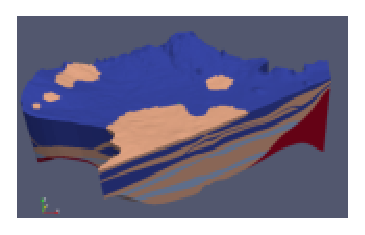
\includegraphics[scale=1]{figures/intro4}
\caption{Nankou groundwater quality model \cite{SunEtAl2010}}
\label{fig:apl5}
\end{minipage}
\end{figure}

%-------------------------------------------------------------------------

\begin{figure}[!htb]
\begin{minipage}[t]{0.48\textwidth}
\subsection{Energy storage}

A very recent research area for THMC modelling became energy storage. The economy and feasibility of renewable energy sources will depend on a large degree on efficient energy storage systems. Fig. \ref{fig:apl6} shows the numerical simulation of flow and heat distribution in a solid thermal energy storage block which will be used to store solar energy collected during days for use at nights (so called solar-thermics). The long term stability and efficiency of those energy storage devices can be optimized using THMC modelling (i.e. solving the inverse geothermal problem). In addition to thermal storage, thermo-chemical concepts are under development, i.e. storing thermal energy by triggering endothermic reactions and gaining thermal energy back on demand with the reverse reaction (exothermic).
\end{minipage}
\hspace{0.02\textwidth}
\begin{minipage}[t]{0.48\textwidth}
%\vspace{4.5cm}
\vspace{1.5cm}
\includegraphics[scale=0.3]{figures/intro5}
\caption{Optimizing energy storage concepts by modelling (OGS simulation by Wenqing Wang), \cite{HGFEnergy:2010}}
\label{fig:apl6}
\end{minipage}
\end{figure}

\label{sec:introduction}
%-------------------------------------------------------------------------
\chapter*{Part I \\[5mm] Theory and Numerics}
\thispagestyle{empty}
\addcontentsline{toc}{chapter}{Part I - Theory and Numerics}
\chapter*{Symbols}

%\renewcommand{\arraystretch}{1.25}
\begin{table}[htb!]
\caption{Latin symbols}
\label{tab:symbols_latin_a}
%\begin{tabular}{|l||l|l|}
\begin{tabular}{|p{0.12\textwidth}|p{0.7\textwidth}|p{0.1\textwidth}|}
\hline
Symbol & Meaning & Unit \\
\hline\hline
$c_p$ & Isobaric heat capacity &  \\
$c_v$ & Isochoric heat capacity &  \\
$\fourtens{C},C_{ijkl}$ & Consistent material tensor & \\
$C$ & Concentration & $kgm^{-3}$ \\
$C_S$ & Sorbed concentration & $kgkg^{-1}$ \\
$d$ & Total (material) derivative &  \\
$\mathbf{d} = \miu{\varepsilon}{}{\dot}$ & Strain rate tensor &  \\
$\mathbf{D}$ & Hydrodynamic dispersion tensor & \\
$e$ & Energy density & $J/kg$ \\
$\miu{e}{i}{}$ & Cartesian base vectors, $i=1,2,3$ &  \\
$E$ & Youngs modulus & $1/Pa$ \\
$\mathbf{f}$ & Force density &  \\
$f$ & Phase distribution function &  \\
$f(\rho,T)$ & Helmholtz free energy &  \\
$\mathcal{F}$ & Resultant force &  \\
$\mathbf{g}$ & Gravity force & $m/s^2$ \\
$G$ & Shear modulus &  \\
$h$ & Piezometric (hydraulic head) & $m$ \\
$h$ & Specific enthalpy & \\
$i$ & Internal energy density & $J~kg^{-1}$ \\
$\mathbf{I}$ & Identity tensor & \\
$\mathbf{j}$ & Flux density & \\
$\mathbf{k}$ & Permeability tensor & $m^2$ \\
$K$ & Bulk modulus & \\
$m$ & Mass density & $kg/m^3$ \\
$M$ & Mass & \\
$n$ & Porosity & $m^3/m^3$ \\
$\mathbf{n}$ & Normal vector &  \\
$p$ & Pressure & $Pa$ \\
$p_c$ & Capillary pressure & $Pa$ \\
$\mathcal{P}$ & Material point &  \\
\hline
\end{tabular}
\end{table}
%\renewcommand{\arraystretch}{1.00}

\clearpage

%\renewcommand{\arraystretch}{1.25}
\begin{table}[htb!]
\caption{Latin symbols (cont.)}
\label{tab:symbols_latin_b}
%\begin{tabular}{|l||l|l|}
\begin{tabular}{|p{0.12\textwidth}|p{0.7\textwidth}|p{0.1\textwidth}|}
\hline
Symbol & Meaning & Unit \\
\hline\hline
$q$ & Source/sink term density &  \\
$Q$ & Source/sink term &  \\
$R$ & Gas constant &  \\
$s$ & Entropy & \\
$S$ & Saturation & $m^3/m^3$ \\
$t$ & Time & s \\
$\mathbf{t}$ & Traction (surface force density, Cauchy stress vector) &  \\
$T$ & Temperature & $K$ \\
$\mathbf{u}$ & Displacement vector & m \\
$\bar {\mathbf{u}} $ & Displacement vector & m \\
$\mathbf{x}$ & Position vector & m \\
$x_1,x_2,x_3$ & Cartesian coordinates & m \\
$\mathbf{X}$ & Reference position vector & m \\
$\mio{v}{}{}$ & Seepage velocity & $m/s$ \\
$\mathbf{v}$ & Velocity vector & $m~s^{-1}$ \\
$v$ & Partial volume & $m^3$ \\
$V$ & Volume & $m^3$ \\
$V_m$ & Molare volume & \\
$\mio{w}{}{}$ & Darcy (filter) velocity & $m/s$ \\
$\mathbf{w}$ & Interface velocity vector & $m~s^{-1}$ \\
\hline
\end{tabular}
\end{table}
%\renewcommand{\arraystretch}{1.00}

\clearpage

\begin{table}[htb!]
\caption{Greek symbols}
\begin{tabular}{|p{0.12\textwidth}|p{0.7\textwidth}|p{0.1\textwidth}|}
\hline
Symbol & Meaning & Unit \\
\hline\hline
% Greek symbols
$\alpha$ & Phase indicator & \\
$\alpha_L$ & Longitudinal dispersivity & $m$ \\
$\alpha_T$ & Transverse dispersivity & $m$ \\
$\alpha_T$ & Thermal expansion coefficient & $1/K$ \\
$\gamma$ & Fluid phase indicator &  \\
$\Gamma$ & Model domain surface &  \\
$\delta _{ij}$ & Kronecker symbol &  \\
$\epsilon$ & Volume fraction &  \\
$\miu{\varepsilon}{}{}$ & Strain tensor &  \\
$\miu{\varepsilon}{d}{}$ & Deviatoric strain tensor &  \\
$\miu{\varepsilon}{v}{}$ & Volumetric strain tensor &  \\
$\eta$ & Viscosity & \\
$\theta$ & Moisture content & $m^3/m^3$ \\
$\lambda$ & Pore size distribution index & \\
$\lambda$ & Lam� constant & \\
$\lambda$ & Thermal conductivity & \\
$\lambda_c$ & Creep multiplier & \\
$\lambda$ & Filtration coefficient & $m^(-1)$ \\
$\mu$ & Dynamic viscosity & \\
$\mu$ & Lam� constant & \\
$\nu$ & Poisson ratio & \\
$\rho$ & Material density & $kg/m^3$ \\
$\miu{\sigma}{}{}$ & Cauchy stress tensor &  \\
$\miu{\tau}{}{}$ & Kirchhoff stress tensor &  \\
$\phi$ & Individual constitutent & \\
$\mathbf{\Phi}$ & Flux vector & \\
$\Phi_{\mathrm{c}}$ & Creep potential &  \\
$\Phi_{\mathrm{pl}}$ & Plastic potential &  \\
$\chi$ & Effective stress parameter & \\
$\psi$ & General intensive conservation quantity &  \\
$\Psi$ & General extensive conservation quantity &  \\
$\omega$ & Gravimetric water content &  \\
$\omega$ & Acentric factor &  \\
$\Omega$ & Control volume, representative elementary volume (REV) & \\
\hline
\end{tabular}
\end{table}

\begin{table}[htb!]
\caption{Math symbols}
\begin{tabular}{|p{0.12\textwidth}|p{0.7\textwidth}|p{0.1\textwidth}|}
\hline
Symbol & Meaning & Unit \\
\hline\hline
% Math symbols
$\mathrm{tr}$ & Trace of ... &  \\
$\nabla()$ & Gradient operator &  \\
$\nabla\cdot()$ & Divergence operator &  \\
$\partial$ & Partial differential &  \\
$\otimes$ & Dyadic product &  \\
% Exponents, suffixes
\hline
$A^T$ & Transpose of ... & \\
$A_{ij}$ & Tensor components &  \\
$\dot A$ & Time derivative & $s^{-1}$ \\
$A_k$ & k component (e.g. chemical species) &  \\
$A'$ & Fluctuation of a quantity & \\
$\bar{A}$ & Mean value of a quantity & \\
$A^\alpha$ &  &  \\
$A_{sw}$ & Swelling property &  \\
$A_{eff}$ & Effective property &  \\
$A^{\alpha R}$ & Material phase property &  \\
$A_{r}$ & Residual property &  \\
$A^{w}$ & Wetting property &  \\
$A^{nw}$ & Non-wetting property &  \\
$A_{el}$ & Elastic property &  \\
$A_{pl}$ & Plastic property &  \\
$A_{0}$ & Reference property &  \\
$A_{th}$ & Thermal property &  \\
$A_{ex}$ & Excess property &  \\
$A_{c}$ & Critical property (at critical point) &  \\
$\mio{A}{}{}$ & Vector & \\
$\mathbf A$ & Tensor & \\
\hline
\end{tabular}
\end{table}

ToDo
\begin{itemize}
	\item Eqn or equation
	\item $\psi$ or $\varphi$
	\item $q$ or $w$ (interface velocity)
\end{itemize}

\chapter{Theory  \today}
\label{cha:theory}
\textit{by Olaf Kolditz, Norbert B�ttcher and Uwe-Jens G�rke}

Concerning the theoretical background of flow, transport, deformation, and reaction processes in porous media,
there is a considerable amount of monographic literature available \cite{Bea:72,Die:85,Ehl:89,BeaBac:90,Kin:1992,Hel:97,LewSch:98,Boe:00}.
%
The idea of this chapter is to provide a concise brief-as-possible description (compendium-like) of governing equations for thermo-hydro-mechanical / chemical [THM/C] processes in porous media. We will point to literature references rather than giving detailed derivations of the governing equations. This part is the theoretical basis for all benchmarks and examples upcoming in part II and III of this book. We will refer to this part in the examples sections where the working equations are briefly repeated. A list of symbols can be found in the Appendix.

From the mechanical point of view we consider non-isothermal flow of multiple fluid phases (compressible and incompressible fluids) in a deformable thermo-poro-elastic porous medium based on Biot's consolidation concept.
A short introduction to continuum mechanics is given in section \ref{sec:continum_mechanics},
followed by basic conservations principles (section \ref{sec:conservation_principles}) as well as an introduction to theory of porous medium (section \ref{sec:porous_medium}).
%
The followings steps are conducted to derive the general field equations:
\begin{itemize}
 \item Macroscopic balance equations for mass, momentum and energy conservation of porous media (section \ref{sec:balance_equations}),
 \item Constitutive relationships for non-isothermal multiphase flow and deformation processes in porous media, 
 (sections \ref{sec:fluid_properties} and \ref{sec:m_properties}),
 \item Applying the constitutive relationships and introducing physically based simplifications to the balance equations for the derivation of the general field equations. 
 (parts II and III).
\end{itemize}

%-------------------------------------------------------------------------
\section{Continuum mechanics}
\label{sec:continum_mechanics}
%\section{Continuum mechanics}

The basic idea of continuum mechanics is
that the evolution of a physical system is completely determined by conservation laws,
i.e. basic properties such as mass, momentum, and energy are conserved
during the considered process at all times.
Any physical system can be completely determined by these conservation properties.
In contrast,
other quantities such as pressure or entropy do not obey conservation laws.
The only additional information concerns the consistence of the material
(e.g. fluids, solids, porous medium) in form of constitutive laws.

The concept of conservation means
that the variation of a conservation quantity within a given control volume
is due to the net effect of internal {\it sources} and
of the amount of the quantity which is crossing the boundary surface
of the considered volume - {\it fluxes}.
Sources and fluxes are, in general, dependent of space-time coordinates as well as
on mechanical and thermodynamic factors.
Fluxes result from two contributions:
first due to advective transport by fluid motion and
second due to diffusion/dispersion processes.
Diffusion is always present even when the fluid is at rest.
Diffusion is the tendency towards equilibrium or homogeneity
of a physical system.

%-------------------------------------------------------------------------
%\subsection{Preliminary remarks}
%\label{sec:prelim}

The mechanical description of coupled thermo-hydro-mechanical (THM) processes in porous media is closely associated with the deformation of the solid phase, and the interaction of deformation and flow processes. Each solid material body (including the solid phase of a porous medium) can exhibit different kinds of motion (section \ref{sec:kinematics}):

\begin{itemize}
\item rigid body motion (translation or rotation of the body without changing its volume or shape), and
\item deformation (local relative change of lengths and/or angles referred to neighboring particles, resulting in variations of the shape and/or volume of the material body under consideration).
\end{itemize}

Deformation processes of a porous medium interact with hydraulic processes of the coupled physical system particularly in the following way:

\begin{itemize}
\item effects on the stress state within the solid phase due to pore pressure evolution (with possible risk of rock failure), and
\item variations of the pore size distribution due to the deformation of the solid skeleton, which affect the hydraulic properties, and thus, have an impact on the flow processes in the porous medium.
\end{itemize}

The analysis of deformation processes considered as mechanical response of the material body to the action of applied external forces is one of the objects of mechanics (micromechanics, continuum mechanics, CITATIONS). Porous media distinguish themselves by a sophisticated complex microstructure, whose realistic simulation is extremely challenging, and from a practical point of view generally not efficient. Therefore, continuum mechanics (which is based on the assumption that matter is continuously distributed in space) provides the preferred approaches for the mathematical modeling of deformation processes in porous media. Appropriate models are not based on a physical characterization of the real microstructure, but consider their effects on the physical behavior in a phenomenological manner (section \ref{sec:porous_medium}).

General statements of mechanics, which are independent of the specific material under consideration, refer to the kinematics of motion (shortly described in a following section) and the balance relations (section~\ref{sec:balance_equations}). By contrast, individual material dependent statements refer to the constitutive relations (section.~\ref{sec:m_properties}). Just both the balance relations as well as the constitutive relations constitute a mathematically closed system of equations to solve initial-boundary value problems of mechanics.

%-------------------------------------------------------------------------
%\section{Kinematics of continua}

% *** EPS-Grafik ***
\begin{figure}[htb!]
\begin{center}
\footnotesize
%\includegraphics[height=5.973cm,width=11.507cm]{../figures/figure1.bmp}
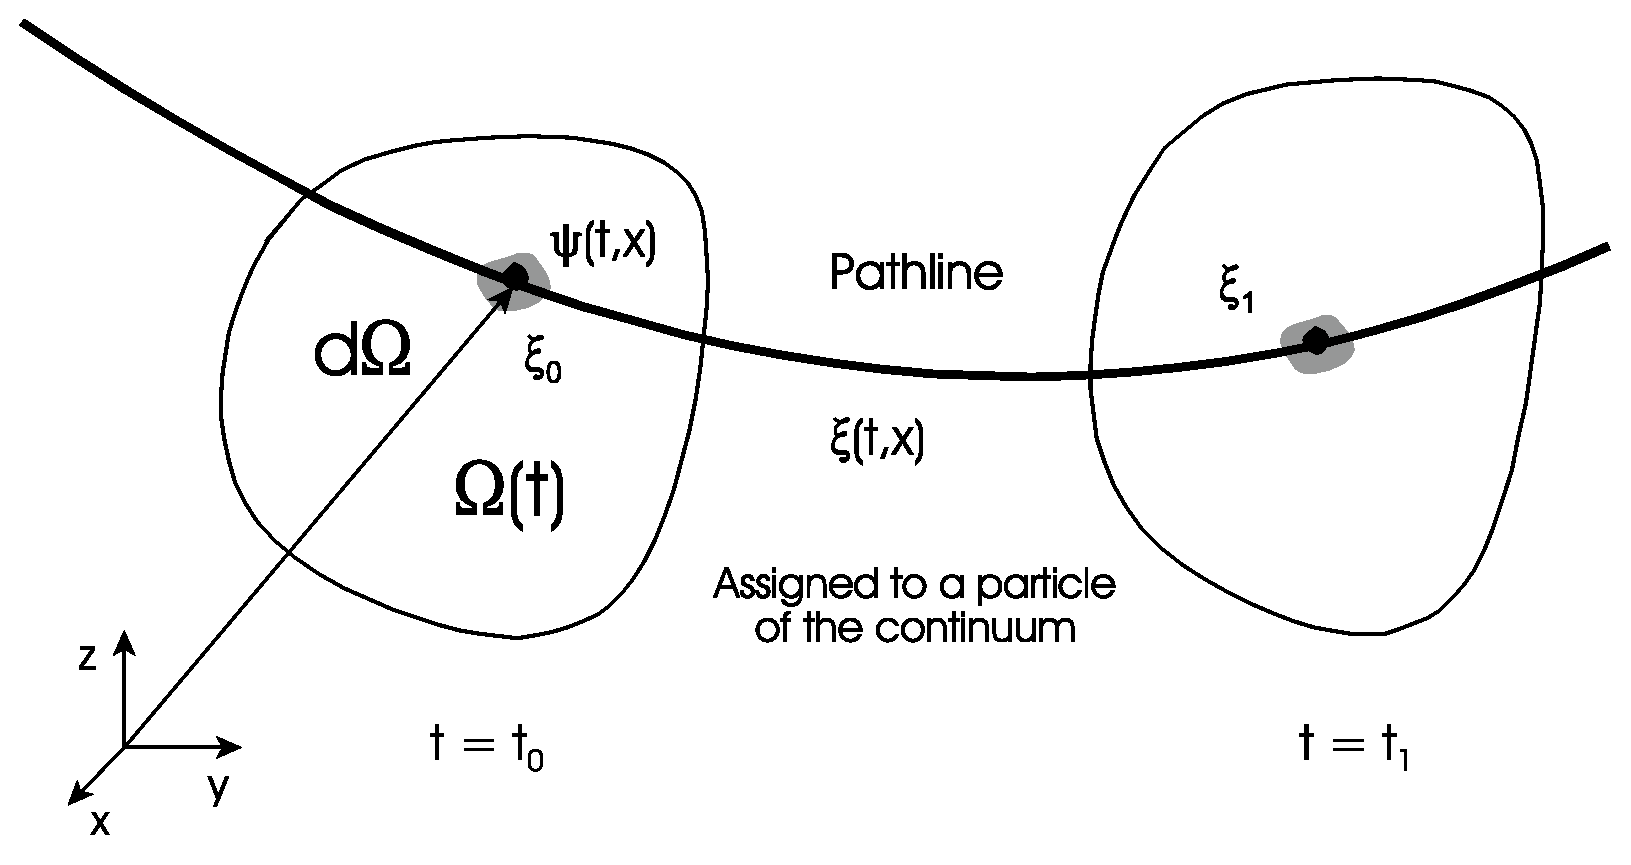
\includegraphics[width=0.8\columnwidth]{figures/mech1.eps}
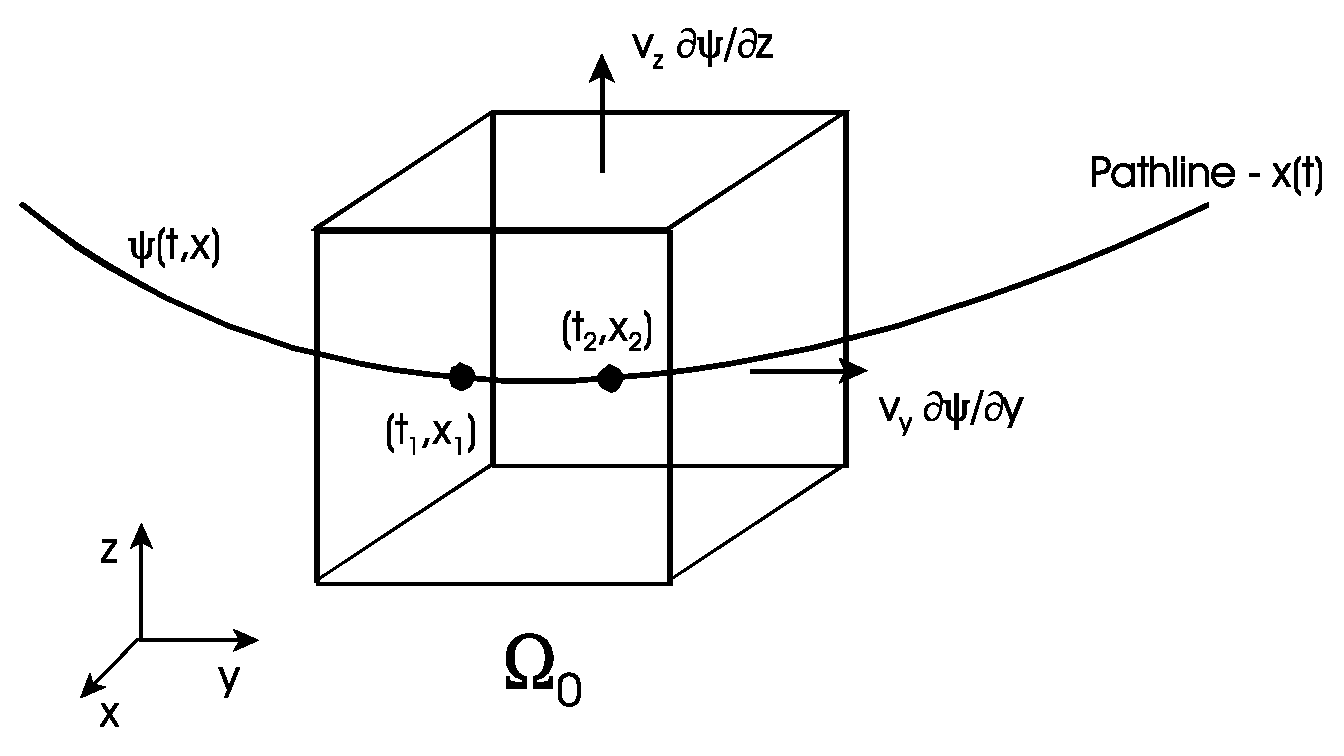
\includegraphics[width=0.8\columnwidth]{figures/mech2.eps}
\caption{Two basic descriptions of motion - Langrangian (top) and Eulerian principles (bottom), adopted from \cite{Kol:02}}
\label{fig:Euler-Langrange}
\end{center}
\end{figure}

\subsection{Lagrangian and Eulerian principles}
\label{sec:euler_lagrange}

In the {Lagrangian formulation}\index{formulation - Lagrangian} we
follow the quantity along a pathline, i.e. following particles
(Fig. \ref{fig:Euler-Langrange}, top). In the {Eulerian
formulation}\index{formulation - Eulerian} of motion we consider
variations of the quantity with respect to a fixed control
volume\index{volume - control} at fixed places (Fig.
\ref{fig:Euler-Langrange}, bottom).

A {pathline}\index{flow - pathline} is a curve along which a fixed
particle of a continuum moves during a sequence of time. Pathline
is Lagrangian concept of motion. A
{streamline}\index{flow - streamline} is a curve along which a
sequence of particles moves at a given time. By definition, the
tangent to a streamline coincides with the velocity vector at that
point. Streamline is Eulerian concept of motion. Note, for
unsteady flow the streamline may vary from one instant to the
next, whereas for steady flow streamlines remain unchanged with
time. For steady motion both pathlines and streamlines coincide.
Any particle will remain on a given streamline as time proceeds.
Additional terms associated with kinematics of continua are the
following (see also section \ref{sec:kinematics}).

\subsection{Kinematics of continua}
\label{sec:kinematics}

Kinematics analyzes the geometry of motion in general, and of deformation processes in particular. It is based on the assumption that a material (physical) body $\mathcal{B}$, which represents a set of elements $\mathcal{P}$ called material points (aka: material elements, particles), at each moment of time can be uniquely defined with certain parts (usually different if motion occurs) of space. Assigning the material body particularly to its image in the three-dimensional Euclidean space of physical observations, the location of each material point at each time can be identified with the position vector $\mathbf{x}(t)$ in a physically well-founded manner. Consequently, the position vector can be represented by its Cartesian coordinates $x_1,\,x_2,\,x_3$. In order to characterize the motion of a material body uniquely with respect to a reference state, the domain in space occupied by the material body at an arbitrarily selected time $t_0$ is of an emphasized significance. Usually in porous media mechanics, an appropriately chosen initial state of the solid skeleton is chosen as the reference state. The position vectors to define the positions of the material points at $t_0$ are denoted as $\mathbf{X}$.

\begin{figure}[htb!]
\begin{center}
\footnotesize
\includegraphics[width=0.7\textwidth]{figures/disp_vect.eps}
\caption{Definition of the displacement vector as the difference of the position vectors $\mathbf{x}$ and $\mathbf{X}$ of a material point (particle) of the body under consideration at various time $t$ (current time) and $t_0$ \cite{Haupt:2002}}
\label{fig:disp_vect}
\end{center}
\end{figure}

One of the primary variables within the context of the numerical simulation of coupled THM processes is the displacement vector $\mathbf{u}$ of the solid phase. The displacement vector is a commonly used kinematic variable to describe the motion (rigid body motion and/or deformation) of a solid material, and quantifies the change in the position of a given material point (cf. Fig.~\ref{fig:disp_vect}).
\begin{equation}
\mathbf{u}(\mathbf{X},t)\,=\,\mathbf{x}(\mathbf{X},t)\,-\,\mathbf{X}
\label{eq:defvec}
\end{equation}
In other words: the displacement vector connects the current position $\mathbf{x}$ of a material point which under the impact of external forces has been moved, and was located at time $t_0$ at the position $\mathbf{X}$. As, in general, the displacement vector will vary locally and temporally, $\mathbf{u}(\mathbf{X},t)=\mathbf{u}(\mathbf{X}(\mathbf{x},t),t)=\bar{\mathbf{u}}(\mathbf{x}{}{},t)\equiv\mathbf{u}$ represents a vector field as function of space and time.

For the sake of the possible comparison of the response of material bodies, which are composed of different materials and/or have a different geometry, to the impact of external forces it is not reasonable to deal with the physically obvious variables displacement and force, but rather to introduce relative physical variables like strain and stress measures. Strain measures represent second-order kinematic tensor variables characterizing the local deformation processes, which deviate from the rigid body motion of a material body.

Based on the definition of the displacement gradient
\begin{equation}
\nabla{\bar{\mathbf{u}}}(\mathbf{x},t)\,=\,\frac{\partial u_i}{\partial x_j}\,\miu{e}{i}{}\otimes\miu{e}{j}{}
\label{eq:dispgrad}
\end{equation}
with the orthonormal system of Cartesian base vectors $\miu{e}{i}{}$ ($i=1,2,3$), the strain tensor $\miu{\varepsilon}{}{}(\mathbf{x},t)$ in case of small (infinitesimal) deformations is established as the symmetric part of the displacement gradient.
\begin{equation}
\miu{\varepsilon}{}{}(\mathbf{x},t)\,=\,\frac{1}{2}
\left(\nabla{\bar{\mathbf{u}}}(\mathbf{x},t)\,+\,\left(\nabla{\bar{\mathbf{u}}}(\mathbf{x},t)\right)^{\mathrm{T}}\right)
\label{eq:straintens}
\end{equation}

The matrix of the coefficients of the strain tensor consists of so-called normal components
\begin{equation}
\varepsilon_{ii}\,=\,\frac{\partial u_i}{\partial x_i}
\label{eq:straintensnormal}
\end{equation}
and shear components.
\begin{equation}
\varepsilon_{ij}\,=\,
\frac{1}{2}\left(\frac{\partial u_i}{\partial x_j}\,+\,\frac{\partial u_j}{\partial x_i}\right)
\qquad(i\neq{j})
\label{eq:straintensshear}
\end{equation}
For special cases it can be easily shown that normal strain is geometrically interpreted as elongation of material line elements (Fig.~\ref{fig:extension}),
\begin{figure}[htb!]
\begin{center}
\footnotesize
\includegraphics[width=0.7\textwidth]{figures/extension.eps}
\caption{Extension (normal strain) of a material line element $d\mathbf{X}=\vert d\mathbf{X}\vert\miu{e}{}{}$
\cite{Haupt:2002}}
\label{fig:extension}
\end{center}
\end{figure}

and shear strain represents the change of the angle between two material line elements, which initially were perpendicular to each other (Fig.~\ref{fig:shear}).
\begin{figure}[htb!]
\begin{center}
\footnotesize
\includegraphics[width=0.7\textwidth]{figures/shear.eps}
\caption{Shear (shear strain) of two material line elements $d\mathbf{X}_1=\vert d\mathbf{X}_1\vert\miu{e}{1}{}$ and $d\mathbf{X}_2=\vert d\mathbf{X}_2\vert\miu{e}{2}{}$, which are orthogonal in the undeformed state \cite{Haupt:2002}}
\label{fig:shear}
\end{center}
\end{figure}

For the analysis of certain deformation processes it is reasonable to consider local volume changes and shape changes separately. Within this context, the strain tensor can be additively split into two parts: a volumetric $\miu{\varepsilon}{v}{}$ and a so-called deviatoric (volume-preserving) $\miu{\varepsilon}{d}{}$ one.
\begin{equation}
\miu{\varepsilon}{}{}\,=\,\miu{\varepsilon}{d}{}\,+\,\miu{\varepsilon}{v}{}
\label{eq:strainsplit}
\end{equation}
The individual partial strain tensors are defined as follows:
\begin{eqnarray}
\miu{\varepsilon}{v}{} & = & \frac{1}{3}\mathrm{tr}(\miu{\varepsilon}{}{})\,\mathbf{I}\,=\,
\frac{1}{3}(\varepsilon_{11}+\varepsilon_{22}+\varepsilon_{33})\,\mathbf{I}
\label{eq:devstrain}
 \\[2.0ex]
\miu{\varepsilon}{d}{} & = & \miu{\varepsilon}{}{}\,-\,\miu{\varepsilon}{v}{}
\label{eq:volstrain}
\end{eqnarray}

Based on the definition
\begin{equation}
\mathbf{v}^s(\mathbf{x},t)\,=\,\mathop{\bar{\mathbf{u}}}\limits^{\miu{.}{}{}}(\mathbf{x},t)
\label{eq:solidveloc}
\end{equation}
of the velocity of material points of the solid skeleton, the strain rate tensor
\begin{equation}
\miu{\varepsilon}{}{\dot}(\mathbf{x},t)\,=\,\mathbf{d}(\mathbf{x},t)\,=\,\frac{1}{2}
\left(\nabla\mathbf{v}^s(\mathbf{x},t)\,+\,\left(\nabla\mathbf{v}^s(\mathbf{x},t)\right)^{\mathrm{T}}\right)
\label{eq:strainratetens}
\end{equation}
with its coefficients
\begin{equation}
d_{ij}\,=\,
\frac{1}{2}\left(\frac{\partial v^s_i}{\partial x_j}\,+\,\frac{\partial v^s_j}{\partial x_i}\right)
\label{eq:strainratecoeff}
\end{equation}
can be defined, which is necessary for the investigation of deformation processes in case of rate-dependent material behavior.

In case of small strains, which was assumed here, the relation between the strain tensor and the displacement vector is a linear one (see section (\ref{eq:straintens})). Considering large strains, the definition of appropriate strain measures requires more sophisticated reflections about the kinematics of motion. As a result, different strain tensors can be obtained representing non-linear functions of the displacement vector. 

%-------------------------------------------------------------------------
\subsection{Stress Tensor}
\label{sec:stresstensor}

The momentum as well as the moment of momentum of a material body are affected by external forces acting on it, which represent the mechanical effect of the surroundings (cf. Fig.~\ref{fig:ext_forces}). Summarizing all local forces, the resultant force $\mathcal{F}$ can be defined.
\begin{equation}
\mathcal{F}\,=\,
\int\limits_{\partial\mathcal{B}}\mathbf{t}\,da\,+\,\int\limits_{\mathcal{B}}\mathbf{f}\,dm\,=\,
\int\limits_{\Gamma}\mathbf{t}(\mathbf{x},t,\mathbf{n})\,d\Gamma\,+\,
\int\limits_{\Omega}\mathbf{f}_v(\mathbf{x},t)\,\varrho(\mathbf{x},t)\,d\Omega
\label{eq:result_force}
\end{equation}
Generally, the material body under consideration bears forces distributed over its surface with the surface force
density $\mathbf{t}$ (traction, Cauchy stress vector), and forces distributed over the volume of the material body with the volume force density (mass distributed specific volume force) $\mathbf{f}_v$. As mentioned above, only gravity $\varrho\mathbf{g}$ should be considered as specific volume force.

\begin{figure}[htb!]
\begin{center}
\footnotesize
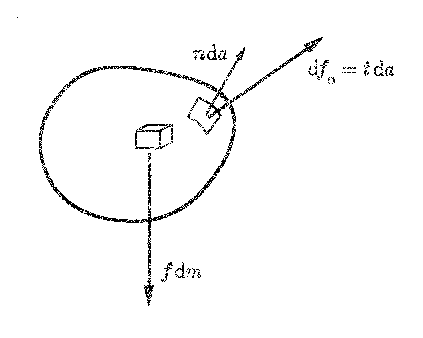
\includegraphics[width=0.6\textwidth]{figures/ext_forces.eps}
\caption{External volume and surface forces acting on infinitesimal geometrical elements of a material body \cite{Haupt:2002}}
\label{fig:ext_forces}
\end{center}
\end{figure}

The traction vector $\mathbf{t}(\mathbf{x},t,\mathbf{n})$ is considered to be a function of the location of its action on the surface, a function of time and of the normal vector, which characterizes the orientation of the surface element $d\miu{\Gamma}{}{}$. Assuming a linear relation between the traction and the normal vector (Cauchy's theorem), the stress measure $\miu{\sigma}{}{}(\mathbf{x},t)$ (Cauchy stress tensor) is defined as a link between surface traction and surface orientation. 
\begin{equation}
\mathbf{t}(\mathbf{x},t,\mathbf{n})\,=\,\miu{\sigma}{}{}(\mathbf{x},t)\,\mathbf{n}
\qquad\Rightarrow\qquad
\miu{\sigma}{}{}\,=\,\sigma_{ij}\,\miu{e}{i}{}\otimes\miu{e}{j}{}
\label{eq:cauchy_theorem}
\end{equation}
Based on Cauchy's theorem, the differential surface force $d\mathbf{f}_0$ acting on a surface element can be obtained. 
\begin{equation}
d\mathbf{f}_0\,=\,\mathbf{t}\,d\Gamma\,=\,(\miu{\sigma}{}{}\,\mathbf{n})\,d\Gamma\,=\,
\miu{\sigma}{}{}\,(\mathbf{n}\,d\Gamma)\,=\,\miu{\sigma}{}{}\,d\miu{\Gamma}{}{}
\label{eq:differ_surforce}
\end{equation}

For certain cases it is reasonable to use the so-called Kirchhoff stress tensor $\miu{\tau}{}{}$, a weighted Cauchy stress measure, instead of the Cauchy stress tensor itself.
\begin{equation}
\miu{\tau}{}{}\,=\,\frac{\varrho_0}{\varrho}\,\miu{\sigma}{}{}
\end{equation}

The second-order stress tensor characterizes the local internal load state referring to a material point of the body under consideration. Generally, it can be defined by three stress vectors acting on three faces of an infinitesimal tetrahedron, which are perpendicular to each other analyzing the equilibrium of forces for this domain. The coefficients of the resulting stress tensor are denoted by two indices -- the first indicates the direction of the normal vector of the face under consideration, the second one the direction of the stress coefficient (see Fig.~\ref{fig:stresstens_plane} for the three-dimensional case).

%\begin{figure}[htb!]
%\begin{center}
%\footnotesize
%\includegraphics[width=0.6\textwidth]{figures/cauchy_law.png}
%\caption{Equilibrium of surface tractions acting on the edges of an infinitesimal triangular element. Definition of %the Cauchy stress tensor using Cauchy's theorem (Jaeger et al. \cite{JCZ:2007})}
%\label{fig:cauchy_law}
%\end{center}
%\end{figure}

\begin{figure}[htb!]
\begin{center}
\footnotesize
%\includegraphics[width=0.6\textwidth]{figures/stresstens_plane.eps}
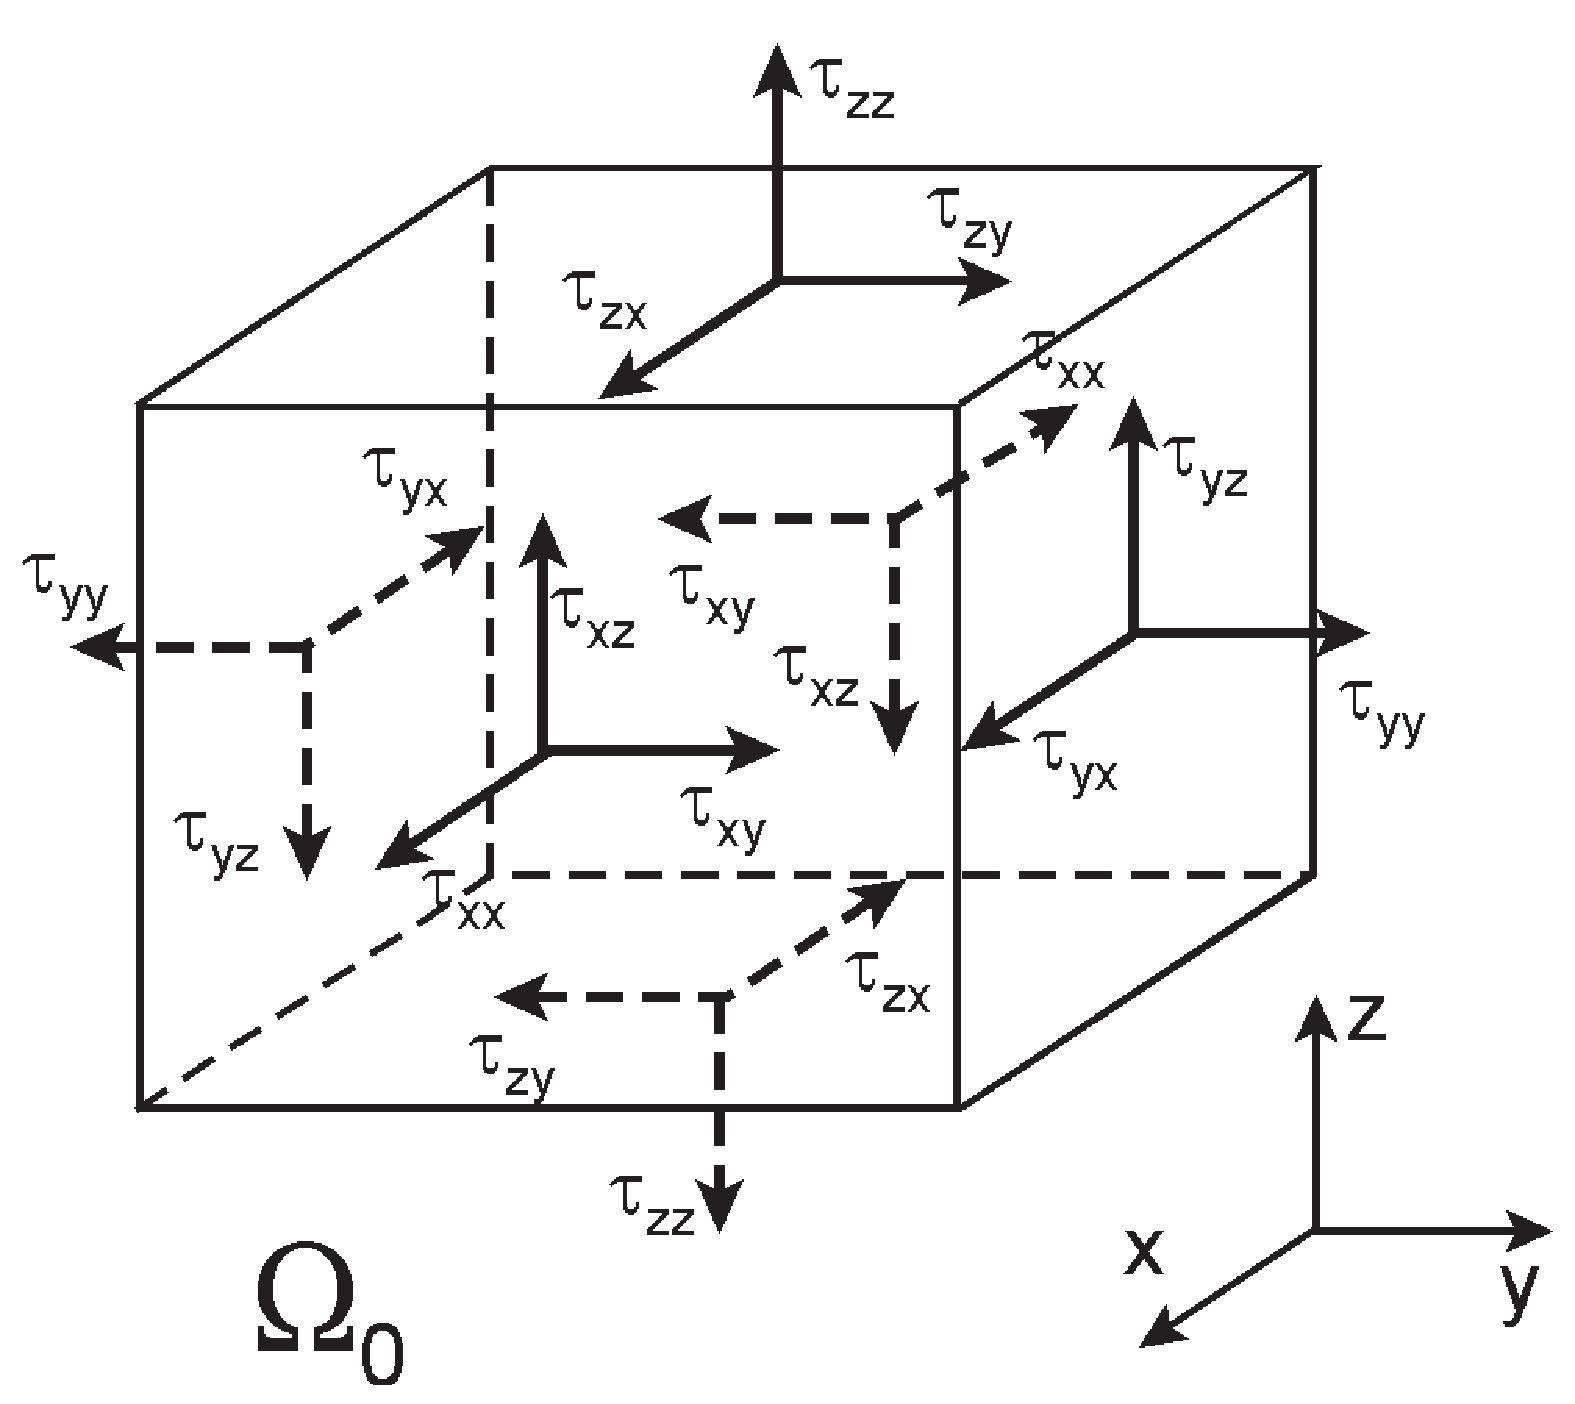
\includegraphics[width=0.6\textwidth]{figures/mech5.eps}
\caption{Coefficients of the stress tensor acting on a small hexahedral element \cite{Kol:02}}
\label{fig:stresstens_plane}
\end{center}
\end{figure}

The sign convention, usually applied in continuum mechanics, implies positive stress coefficients coinciding with the directions of the axes of coordinates at faces with normal vectors also coinciding with the directions of the axes of ccordinates. Consequently, tensile stress coefficients are positive, compressive stresses negative. Positive stress coefficients on opposite faces are oppositely directed (but of equal absolute value). The matrix of the coefficients of the (Kirchhoff) stress tensor is composed as follows:
\begin{equation}
\tau_{ij}\,=\,
\left(
\begin{array}{ccc}
\tau_{xx} & \tau_{xy} & \tau_{xz} \\
\tau_{yx} & \tau_{yy} & \tau_{yz} \\
\tau_{zx} & \tau_{zy} & \tau_{zz}
\end{array}
\right)
\label{eq:stress_matrix}
\end{equation}
Analogous to the strain tensor, the coefficients $\tau_{xx},\,\tau_{yy},\,\tau_{zz}$ are called normal stresses, the coefficients $\tau_{ij}\quad(i\neq j)$ shear stresses with $\tau_{ij}=\tau_{ji}$ (symmetry of the stress tensor, which results from the balance of moment of momentum).

In the special uniaxial stress case only at one face of a volume element a normal stress occurs, whereas all the other faces are stress-free. Consequently, the stress coefficient is calculated as the force acting on the face under consideration divided by its area.








%-------------------------------------------------------------------------
\subsection{Conservation principles}
\label{sec:conservation_principles}
%\section{Conservation principles}

\footnote{Truesduell}

Based on the kinematical foundation (section \ref{sec:kinematics}) we formulate the general conservation principle of continuum mechanics for both Eulerian and Lagrangian points of view (section \ref{sec:euler_lagrange}).
%
The amount of a (conservation) quantity in a defined volume $\Omega$ is given by

\begin{eqnarray}
\Psi =
\int\limits_\Omega \psi d\Omega(t)
\end{eqnarray}

where $\Psi$ is an extensive conservation quantity\index{quantity
- extensive } (i.e. mass, momentum, energy) and $\psi$ is the
corresponding intensive conservation quantity\index{quantity -
intensive} such as mass density $\rho$, momentum density $\rho \bf
v$ or energy density $e$ (see Table
\ref{tab:conservation_quantities}).

%
\begin{table}[htb!]
\caption{Conservation quantities}
\label{tab:conservation_quantities}
\begin{center}
\begin{tabular}{|ll|ll|}
\hline
Extensive  quantity &  Symbol    &  Intensive quantity      &  Symbol  \\
\hline \hline
%\mbox{\rule[1mm]{0cm}{3mm}Mass}
Mass                &  $M$,$M_k$ & Mass density             & $\rho$,$\rho_k$  \\
Linear momentum     &  $\bf m$   & Linear momentum density  & $\rho \bf v$ \\
Energy              &  $E$       & Energy density           & $e = \rho i + \frac 1 2 \rho v^2 $
\\[1pt]
\hline
\end{tabular}
\end{center}
\end{table}
%

The balance equations for mass, momentum and energy conservation can be derived based on two fundamental principles, i.e. Eulerian and Lagrangian frameworks (e.g. \cite{Kol:02})
%
Both conservation principles are related by two different forms of derivatives
\begin{equation}
\frac{d \psi}{dt}
=
\frac{\p \psi}{\p t} + \v\cdot\nabla\psi
\label{eqn:derivatives}
\end{equation}
the total (or material) $d$ and partial derivatives $\p$, respectively.
%
The general integral balance equation is given by
%
\begin{eqnarray}
\frac{d}{dt} \int\limits_\Omega \psi~d\Omega
=
\int\limits_\Omega
\left(
\frac{\partial\psi}{\partial t}
+
\nabla \cdot {\mathbf{\Phi}}
\right)
d\Omega
=
\int\limits_\Omega q^\psi d\Omega
\label{eqn:general_balance_equation}
\end{eqnarray}
%
where $\psi$ is a general conservation quantity, $\mathbf{\Phi}$ is the total flux of $\psi$, and $Q$ is a source/sink term for $\psi$.
%
The corresponding extensive and intensive conservation quantities are summarized in Tab. \ref{tab:conservation_quantities}.

The total flux ${\bf\Phi}^\psi$ of a quantity $\psi$ is defined as
\begin{eqnarray}
{\bf\Phi}^\psi
=
{\bf v}^E \psi
\end{eqnarray}

where ${\bf v}^E$ is a mean particle velocity\index{quantity - velocity -
particle}. Physically ${\bf\Phi}^\psi$ represents the quantity of
$\psi$ passing through a unit area of the continuum, colinear with
${\bf v}^E$, per unit time with respect to a fixed coordinate
syste, i.e. Eulerian point of view.

For the case of a multi-component continuum let ${\bf v}$ denote
the mass-weighted velocity\index{quantity - velocity - mass-weighted}
describing a more ordered motion of the particles of a fluid
element. The total flux can be written as
\begin{eqnarray}
{\bf\Phi}^\psi
=
{\bf v}^E \psi
=
\underbrace{{\bf v} \psi}_{{\bf\Phi}^\psi_A}
+
\underbrace{({\bf v}^E-{\bf v}) \psi}_{{\bf\Phi}^\psi_D}
\end{eqnarray}

and, therefore, decomposed into two parts: an advective flux
${\bf\Phi}^\psi_A$ and a diffusive flux ${\bf\Phi}^\psi_D$
relative to the mass-weighted velocity:

\begin{itemize}
 \item
Advective flux\index{flux - advective} of quantity $\psi$
\begin{eqnarray}
{\bf\Phi}^\psi_A
=
{\bf v}\psi
\end{eqnarray}

 \item
Diffusive flux\index{flux - diffusive} of quantity $\psi$
(Fick's law)\index{law - Fick}
\begin{eqnarray}
{\bf\Phi}^\psi_D=
-\alpha \nabla\psi
\end{eqnarray}
\end{itemize}

where $\alpha$ is a diffusivity coefficient. The negative sign indicates, that diffusive flux is positive in the direction of negative gradient.

If the conservation quantity is a vector (e.g. linear momentum)
then the flux becomes a tensor and the source term a vector (e.g. body forces):

\begin{itemize}

\item Advective flux of vector quantity $\psi$
%
\begin{eqnarray}
{\bf\Phi}^\psi_A
=
% {\bf v}:{\Boldmath\psi}
{\bf v}:{\mathbf{\psi}}
=
\left[
\begin{array}{ccc}
v_x & v_y & v_z
\end{array}
\right]
\left[
\begin{array}{c}
\psi_x \\ \psi_y \\ \psi_z
\end{array}
\right]
=
\left|
\begin{array} {lll}
v_x \psi_x &  v_x \psi_y & v_x \psi_z \\
v_y \psi_x &  v_y \psi_y & v_y \psi_z \\
v_z \psi_x &  v_z \psi_y & v_z \psi_z
\end{array}
\right|
\end{eqnarray}

\item Diffusive flux of vector quantity $\psi$
%
\begin{eqnarray}
{\bf\Phi}^\psi_D
=
% -\rho \nabla:{\Boldmath\psi}
-\rho \nabla:{\mathbf{\psi}}
=
-\alpha
\left|
\begin{array} {lll}
\frac{\partial\psi_x}{\partial x} & \frac{\partial\psi_y}{\partial y} & \frac{\partial\psi_z}{\partial z} \\
\frac{\partial\psi_x}{\partial x} & \frac{\partial\psi_y}{\partial y} & \frac{\partial\psi_z}{\partial z} \\
\frac{\partial\psi_x}{\partial x} & \frac{\partial\psi_y}{\partial y} & \frac{\partial\psi_z}{\partial z}
\end{array}
\right|
\end{eqnarray}
\end{itemize}

When substituting the flux definition into the general balance equation (\ref{eqn:general_balance_equation}),
we yield the so-called transport equation

\begin{eqnarray}
\frac{d}{dt} \int\limits_\Omega \psi~d\Omega
=
\underbrace{\int\limits_\Omega \frac{\partial\psi}{\partial t}~d\Omega}_{1}
+
\underbrace{\int\limits_\Omega \nabla \cdot ({\bf v}\psi)~d\Omega}_{2}
-
\underbrace{\int\limits_\Omega \nabla \cdot (\alpha\nabla\psi)~d\Omega}_{3}
=
\underbrace{\int\limits_\Omega q^\psi}_{4}
\label{eqn:integral_balance_equation}
\end{eqnarray}

with the followind terms:

\renewcommand{\arraystretch}{0.9}
\begin{enumerate}
 \item Rate of increase of $\psi$ within a fluid element
 \item Net rate of $\psi$ due to flux out of the fluid element
 \item Rate of increase / decrease of $\psi$ due to diffusion
 \item Rate of increase / decrease of $\psi$ due to sources
\end{enumerate}

%-------------------------------------------------------------------------
\section{Porous medium}
\label{sec:porous_medium}
%\section{Porous medium}

Soil or rock can be considered as a multiphase medium consisting
of a solid phase (solid matrix) and of one or more fluid phases
(gas and liquids), which occupy the void space (Fig.
\ref{fig:porous_medium}). Fluids are immiscible\index{fluid -
immiscible}, if a sharp interface is maintained between them. In
general, a phase is defined as a part of a continuum, which is
characterized by distinct material properties and by a
well-defined set of thermodynamic state variables. State variables
describe the physical behaviour at all points of the phase. They
must vary continuously within the considered phase of a continuum.
Phases are separated from each other by surfaces referred to as
interphase boundaries. Transport of components may occur within a
phase and/or across interphase boundaries. Those
interphasic\index{process - interphase} exchange processes between
adjacent phases can result from diffusive and/or advective
mechanisms.

In fact, it is impossible to describe the complex geometry of the
solid matrix and the topology of the void space at the microscopic
level, i.e. the topology of the pore space will never be known in
detail. As a consequence, boundary conditions for a mathematical
model cannot be stated at this scale, since they are not known at
the microscopic level. Moreover, it will be extremely difficult to
measure values of state variables at each point within a phase in
order to observe processes, to calibrate and to verify any model.
Finally, the complete formulation and resolution of balance
equations at the microscopic\index{scale - microscopic} level is
impossible and may not be reasonable. Therefore, it is necessary
to transform the problem from a microscopic scale to a
macroscopic\index{scale - macroscopic} level. Starting from the
microscopic balance equations for extensive quantities (masses,
momentum, energy), this procedure is the subject of the theory of
the porous medium 
\cite{Bea:72,Die:85,Ehl:89,BeaBac:90,Kin:1992,Hel:97,LewSch:98,Boe:00}
%(Bear 1972, Diersch 1985, Bear \& Bachmat 1990, de Boer \& Ehlers 1986, Lewis \& Schrefler 1998, de Boer 2000).
The entire problem is rewritten in terms of averages of
microscopic quantities, which have measurable values. The
resulting macroscopic model is referred to as the continuum
approach\index{model - continuum}. This conceptual model implies
that a real system is replaced by a number of overlapping continua
representing the corresponding phases. It is assumed that each
phase, occupying a certain part of the porous domain, is regarded
as a continuum. These individual phases interact with each other
at any place within the entire domain, because they are present at
each point within the porous medium, i.e. all phases are
completely mixed.
%
\begin{eqnarray}
\Omega_0
=
\sum_{\alpha} \Omega^\alpha
\end{eqnarray}
%
In addition to the porous medium approach, there exist different
types of structural models for fractured rocks, which characterize
the degree of inhomogeneity: the fractured medium\index{medium -
fractured} and the fractured porous medium\index{medium - porous
fractured}. The term fractured medium means that only the
fractures are important for the considered process, so blocks
surrounded by the fractures may be neglected in the model. The
term fractured porous medium means that both fracture system and
porous matrix are significant for the considered process. The
domain of a fractured porous medium consists of two subdomains,
representing heterogeneities at different scales, i.e. the
diameter of pores in the matrix and the characteristic length of
fractures.

Appropriate averaging rules must be defined in order to realize
the above described transformation from a microscopic to a
macroscopic level. For this purpose, a well-defined sample size of
an averaging volume must be found, which is referred to as the
representative elementary volume\index{volume - representative
elementary} (abbreviated REV). On the one hand, this averaging
unit has to be sufficiently large, so that the influence of
microscopic inhomogeneity on the values of averaged (macroscopic)
quantities will vanish, i.e. they become independent of size,
shape, and orientation of the REV. On the other hand, the REV must
be small enough to reflect the macroscopic heterogeneity. In
particular, the REV must be much smaller than the domain of
interest, which may vary in size for a flow or a transport
problem, respectively. From the mathematical point of view, the
macroscopic (averaged) quantities must be continuous and
differentiable functions (in space and in time), so that solutions
of the governing differential balance equations can be determined.
Finally, the continuum approach cannot be employed unless a common
range of a REV can be selected for all material properties (e.g.
porosity, permeability, dispersivity) as well as for all relevant
state variables. This requirement is important with respect to the
different conceptual models for fractured rock, which are
introduced in the following.

%=7.2==============================================================================
\subsection{Macroscopic Equations}

%\subsubsection*{Statistic approach}
%\index{model - statistic}

In fact, it is impossible to describe the complex geometry of the solid matrix
and the topology of the void space at the microscopic level, i.e. the topology
of the pore space will never be known in detail. Therefore, a statistical
approach is used for the derivation of balance equations at a macroscopic
level. The physical property of a porous medium is decomposed in phase-related
mean values $\overline{\psi^\alpha}$ and local fluctuations ${\psi'}^\alpha$.
%
\begin{eqnarray}
\psi^\alpha
=
\overline{\psi^\alpha}
+
{\psi'}^\alpha
\end{eqnarray}

%\subsubsection*{Averaging volume}
%\index{scale - averaging - volume}

An appropriate averaging volume is called
the Representative Elementary Volume (REV) (Fig. \ref{rev}).

% *** EPS-Grafik ***
\begin{figure}[htb!]
\begin{center}
\footnotesize
%\psfrag{Synonym}[pos][pos]{Tex-Ersetzung}
%\psfrag{x}[][]{$t$}
%\psfrag{y}[b][t]{$y(t)$}
%\psfrag{t}[][]{ }
%\includegraphics[height=7.5cm,width=11cm]{../figures/fig_71.bmp}
\includegraphics[width=0.95\columnwidth]{figures/por2.eps}  % Filename.eps
\caption{Definition of the representative elementary volume (REV) \cite{BeaBac:90}} 
\label{rev}
\end{center}
\end{figure}
%

%\subsubsection*{Averaging operator}

Several averaging procedures can be defined \cite{BeaBac:90}. As
an example we consider volumetric averaging which is also denoted as the
concept of volume fractions. The volumetric averaging operator is given by
%
\begin{eqnarray}
\overline{\psi^\alpha}^\alpha
=
\frac{1}{\epsilon^\alpha \Omega_0}
\int\limits_{\Omega_0} f^\alpha \psi^\alpha d\Omega
\label{eqn:mean}
\end{eqnarray}

where $\alpha$ is the phase indicator, $\epsilon^\alpha =
\Omega^\alpha/\Omega_0$ is the volumetric fraction of the $\alpha$
phase, $\Omega_0$ is the averaging volume (corresponding to the
representative elementary volume), $f^\alpha=1/0$ (inside or
outside $\alpha$ phase) is the phase distribution function.

%\subsubsection*{Averaging rules}
%\index{scale - averaging - rules}

Due to the above definition the following averaging rules can be derived.

\begin{itemize}
 \item Sum
\begin{eqnarray}
\overline{\psi_1^\alpha+\psi_2^\alpha}
=
\overline{\psi_1^\alpha}+\overline{\psi_2^\alpha}
\end{eqnarray}

 \item Product
\begin{eqnarray}
\overline{\psi_1^\alpha \psi_2^\alpha}
=
\overline{\psi_1^\alpha}\,\overline{\psi_2^\alpha}
+
\overline{{\psi_1'}^\alpha {\psi_2'}^\alpha}
\end{eqnarray}

 \item Time derivative
\begin{eqnarray}
\epsilon^\alpha \overline{\frac{\partial \psi^\alpha}{\partial t}}
=
\frac{\partial \epsilon^\alpha \overline{\psi^\alpha}}{\partial t}
-
\frac{1}{\Omega_0}
\int\limits_{S^{\alpha\beta}}\psi^\alpha {\bf w} \cdot d{\bf S}
\end{eqnarray}

 \item Spatial derivative
\begin{eqnarray}
\epsilon^\alpha \overline{\nabla\psi^\alpha}
=
\nabla(\epsilon^\alpha\overline{\psi^\alpha})
+
\frac{1}{\Omega_0}
\int\limits_{S^{\alpha\beta}}\psi^\alpha \cdot d{\bf S}
\end{eqnarray}

\end{itemize}

where $\bf w$ is the velocity of the $\alpha\beta$-phase interface.

%\subsubsection*{General macroscopic balance equation}
%\index{equation - general balance}

To derive a phase related macroscopic balance equation,
we have to average the balance equation in differential form
for a certain phase (\ref{eqn:general_balance_equation}).
By use of the above averaging operators and rules
the following general macroscopic balance equation
can be obtained.
%
\begin{eqnarray}
\frac{\partial \epsilon^\alpha \overline{\psi^\alpha}}{\partial t}
=
-
\nabla\cdot(
\epsilon^\alpha\bar{\psi^\alpha}\overline{{\bf v}^\alpha}
+
\epsilon^\alpha\overline{{\psi'}^\alpha{\bf v'}^\alpha}
+
\epsilon^\alpha\overline{{\bf\Phi}_{\textrm{\tiny Diff}}^{\psi^\alpha}}
)
\nonumber \\
-
\frac{1}{\Omega_0}
\int\limits_{S^{\alpha\beta}} {\bf\Phi}_{\textrm{\tiny Diff}}^{\psi^\alpha} \cdot d{\bf S}
-
\frac{1}{\Omega_0}
\int\limits_{S^{\alpha\beta}}\psi^\alpha ({\bf v-w}) \cdot d{\bf S}
+
q^{\psi^\alpha}
\end{eqnarray}

with the dispersive flux
\begin{eqnarray}
{\bf\Phi}_{\textrm{\tiny Disp}}^{\psi^\alpha}
=
\epsilon^\alpha\overline{{\psi'}^\alpha{\bf v'}^\alpha}
\end{eqnarray}

%------------------------------
\subsection{Theory of Mixtures}
\label{sec:mixtures}

The Theory of Mixtures as one of the basic approaches to model the complex behavior of porous media has been developed over decades (concerning basic assumptions see e.g. \cite{Bow:1976,TT:1960}). As the Theory of Mixtures does not incorporate any information about the microscopic structure of the material\footnote{Within the context of the Theory of Mixtures the ideal mixture of all constituents of a multiphase medium is postulated. Consequently, the realistic modeling of the mutual interactions of the constituents is difficult.}, it has been combined with the Concept of Volume Fractions by e.g. \cite{Bow:1980,BE:1986a,LewSch:98,Pre:1980}. Within the context of this enhanced Theory of Mixtures (also known as Theory of Porous Media), all kinematical and physical quantities can be considered at the macroscale as local statistical averages of their values at the underlying microscale.
%
Concerning a detailed overview about the history of the modeling of the behavior of multiphase multicomponent porous media, the reader is referred to e.g. \cite{Boe:00}. Comprehensive studies about the theoretical foundation and numerical algorithms for the simulation of coupled problems of multiphase continua are given in e.g. \cite{Boe:00,EB:2002,LewSch:98} and the quotations therein. 

The individual constituents $\varphi^{\alpha}$ of a porous material represent the phases of the overall aggregate or components within a phase. Below, $\alpha=s$ marks one immiscible solid phase (no sorption processes are considered), and $\alpha=\gamma$ denote several immiscible pore fluid phases. 
%
A porous medium, however, consists of multiple phases (fluids such as water, air and non-aqueous phase liquids (NAPLs) as well as solids). 
Moreover, these phases can contain several chemical components which can be dissolved in liquids or adsorbed to the solid phase (Fig. \ref{fig:porous_medium}).

\newpage
.
\vspace{4cm}
\begin{figure}[htbp]
\hspace{3cm}
\includegraphics[width=0.06\columnwidth]{figures/pm}
\caption{Conceptual approach of a porous medium model, adopted from \cite{Kol:02}}
\label{fig:porous_medium}
\end{figure}

Within the framework of the Concept of Volume Fractions, scalar variables like volume fractions and saturations are defined to describe the microstructure of a porous medium in a macroscopic manner neglecting the real topology and distribution of the pores. These variables serve as measures of local fractions of the individual constituents. The volume fractions $n^{\alpha}$ represent the ratio of the partial volume $dv^{\alpha}$ of a given constituent $\varphi^{\alpha}$ of a multiphase body with respect to the overall volume $dv$ of a representative elementary volume (REV) of the control domain $\Omega$ under consideration. Consequently, based on the definitions of the overall volume of the control domain
\begin{equation}
V=\int\limits_{\Omega}\,dv
\label{eq1}
\end{equation}
and the corresponding partial volumes of the individual constituents
\begin{equation}
V^{\alpha}=\int\limits_{\Omega}\,dv^{\alpha}\qquad\mbox{with}\qquad V=\sum\limits_{\alpha}\,V^{\alpha}
\label{eq2}
\end{equation}
the volume fractions
\begin{equation}
n^{\alpha}=\frac{dv^{\alpha}}{dv}
\label{eq3}
\end{equation}
provide some information about the local volume distribution of the individual constituents.
\begin{equation}
V^{\alpha}=\int\limits_{\Omega}\,dv^{\alpha}=\int\limits_{\Omega}\,n^{\alpha}\,dv
\label{eq4}
\end{equation}
One of the most characteristic media properties of a porous material is the porosity, the local amount of fluid volume fractions.
\begin{equation}
n=\sum\limits_{\gamma}\,n^{\gamma}=1\,-\,n^s
\label{eq5}
\end{equation}
Since, in general, the overall medium is completely filled with matter, from Eqn.~(\ref{eq2}) follows the saturation condition regarding the overall aggregate.
\begin{equation}
\sum\limits_{\alpha}\,n^{\alpha}=1
\label{eq6}
\end{equation}

If multiphase flow occurs, it is more convenient for various applications to use the (partial) fluid saturations $S^{\gamma}$ instead of the volume fractions. These local functions are given by
\begin{equation}
S^{\gamma}=\frac{dv^{\gamma}}{dv-dv^s}=\frac{n^{\gamma}}{n}
\label{eq7}
\end{equation}
obviously fulfilling the saturation condition regarding the pore content.
\begin{equation}
\sum\limits_{\gamma}\,S^{\gamma}=1
\label{eq8}
\end{equation}

Usually, constraint conditions addressing real physical effects are formulated to simplify complex mathematical and numerical models. Within the context of porous media, it is reasonable in most applications to assume the (material) incompressibility of constituents as a substantial constraint condition. The issue of (in)compressibility of a material is closely connected to the possible temporal evolution of its mass density.

Within the framework of the Concept of Volume Fractions, two different formulations of mass density related to the constituents of a porous medium are introduced. The so-called material (effective, realistic) density $\rho^{\alpha R}$ is defined as the ratio of the mass fraction $dm^{\alpha}$ of the given individual constituent $\varphi^{\alpha}$ with respect to its partial volume fraction.
\begin{equation}
\rho^{\alpha R}=\frac{dm^{\alpha}}{dv^{\alpha}}
\label{eq9}
\end{equation}
In contrast, the so-called partial (global, bulk) density is given by the ratio of the mass fraction of the constituent under consideration with respect to the volume fraction of the overall aggregate.
\begin{equation}
\rho^{\alpha}=\frac{dm^{\alpha}}{dv}
\label{eq10}
\end{equation}
Based on the definition of the volume fractions (\ref{eq3}), the material and the partial densities are correlated to each other.
\begin{equation}
\rho^{\alpha}=n^{\alpha}\,\rho^{\alpha R}
\label{eq11}
\end{equation}
If the volume fractions change with time under external loading, from Eqn.~(\ref{eq11}) follows that for an intrinsically incompressible individual constituent (constant material mass density) compressibility referred to the overall aggregate is observed.
\begin{equation}
\rho^{\alpha R}=\mbox{const} \quad\Rightarrow\quad
\rho^{\alpha}\,\neq\,\mbox{const}\quad\mbox{as}\quad n^{\alpha}\,\neq\,\mbox{const}
\label{eq12}
\end{equation}

Obviously, the mass density of the porous medium (homogenized overall aggregate) is defined as the sum of the partial densities of its constituents.
\begin{equation}
\rho=\sum\limits_{\alpha}\rho^{\alpha}
\label{eq13}
\end{equation}

The conceptual idea behind the formulations and relations presented above consists in the assumption that the mass fractions of all constituents of the multiphase medium are simultaneously present and statistically uniformly distributed over the entire control domain. Within this context, the material body under consideration is theoretically substituted by an aggregate completely and continuously filled by superimposed (overlapping) homogenized partial continua. In other words, all constituents of a porous medium are characterized as smeared substitute continua with reduced mass densities. Consequently, the motion and physics of the individual constituents as well as the overall aggregate can be specified by well-accepted phenomenological methods of continuum mechanics.

Describing the transport and deformation of the constituents of porous media within the framework of continuum mechanics it is assumed that the geometry of the control domain under consideration is characterized at each time by the solid skeleton, whereas the fluid pore content is able to flow across the boundary of the surface. This assumption serves as conceptual nucleus for the simulation of complex, coupled physical processes in multiphase porous media, particularly if a deformable solid skeleton is observed. Within this context, it proves to be reasonable not to model the absolute motion state of the pore content, but its motion relative to the motion of the solid phase, considering the porous medium as a local thermodynamic open system with the solid skeleton as volume under observation.

The macroscopic characterization of the physical processes considering the real microstructural situation in a statistically averaged manner is completely adequate for the most hydrological, geotechnological and biomechanical problems under consideration (cf. \cite{GWASG:2006} and others).
%-------------------------------------------------------------------------
\section{Balance equations}
\label{sec:balance_equations}
%\section{Balance equations}

We derive the balance equations for phase and component masses as well as for momentum and energy of a porous medium.

\subsection{Phase mass balance}

We consider the mass balance of individual phases of a porous medium.
%
Neglecting mass exchange between the phases (no dissolution and sorption processes), the local mass balance for the individual constituent $\varphi^{\alpha}$ of the porous medium is given by
\begin{equation}
\frac{d_{\alpha}\rho^{\alpha}}{dt}+\rho^{\alpha}\,\nabla\cdot\mio{v}{\alpha}{}=
\frac{\partial\rho^{\alpha}}{dt}+\nabla\cdot\left(\rho^{\alpha}\mio{v}{\alpha}{}\right)=0
\label{eq14}
\end{equation}
with the velocity $\mio{v}{\alpha}{}$ of the constituent under consideration, and the usual divergence operator $\nabla\cdot()$. From the velocity-displacement relation for the solid skeleton follows
\begin{equation}
\mio{v}{s}{}=\mio{u}{s}{\dot}
\label{eq15}
\end{equation}
with the solid displacement vector $\mio{u}{s}{}$. The derivative
\begin{equation}
\frac{d_{\alpha}A}{dt}=\frac{\partial A}{dt}+\mio{v}{\alpha}{}\cdot\nabla A
\label{eq16}
\end{equation}
with the usual gradient operator $\nabla()$ denotes the material time derivative of an arbitrary variable $A$ with respect to the motion of a material point of the constituent $\varphi^{\alpha}$ (cf. equation (\ref{eqn:derivatives})). It consists of a local (diffusive) part and a convective part associated with the velocity of the constituent.

As mentioned above, the transport processes of the fluid constituents of a porous medium are considered as their relative motion with respect to the motion of the deformable solid skeleton. Consequently, the relations between the material time derivatives (here, of an arbitrary variable $A$) with respect to the solid skeleton, and with respect to the individual fluid constituent $\varphi^{\gamma}$ is of crucial interest in terms of a unified numerical characterization of the different processes.
\begin{equation}
\frac{d_{\gamma}A}{dt}=\frac{d_{s}A}{dt}+\mio{v}{\gamma s}{}\cdot\nabla A
\label{eq17}
\end{equation}

Here, 
\begin{equation}
\mio{v}{\gamma s}{}=\mio{v}{\gamma}{}-\mio{u}{s}{\dot}
\end{equation}

is the so-called seepage velocity describing the fluid motions with respect to the deforming skeleton material.

According to the generalized formulation~(\ref{eq14}), considering equations (\ref{eq5}) and (\ref{eq11}), the local solid phase mass balance is given by
\begin{equation}
\frac{d_s\left[(1-n)\rho^{sR}\right]}{dt}+(1-n)\,\rho^{sR}\,\nabla\cdot\mio{u}{s}{\dot}=0
\label{eq18}
\end{equation}

Assuming material incompressibility of the solid phase, i.e. $d_s\rho^{sR}/dt\!\!=\!\!0$ 
we derive the following expression for porosity changes.
\begin{equation}
\frac{d_s n}{dt}
=
(1-n)\,\nabla\cdot\mio{u}{s}{\dot}=0
\label{eq18a}
\end{equation}

Following the same procedure, additionally considering Eqns.~(\ref{eq7}) and (\ref{eq17}), the mass balance relations for the fluid constituents $\varphi^{\gamma}$
can be defined with respect to the solid phase motion.
\begin{equation}
\frac{d_s\left(nS^{\gamma}\rho^{\gamma R}\right)}{dt}+
\nabla\cdot\left(nS^{\gamma}\rho^{\gamma R}\mio{v}{\gamma s}{}\right)+
nS^{\gamma}\rho^{\gamma R}\nabla\cdot\mio{u}{s}{\dot}=0
\label{eq20}
\end{equation}

Applying the solid phase mass balance~(\ref{eq18}), Eqn.~(\ref{eq20}) can be represented in a more detailed description.
\begin{eqnarray}
& & 
nS^{\gamma}\frac{d_s\rho^{\gamma R}}{dt}+n\rho^{\gamma R}\frac{d_sS^{\gamma}}{dt} \nonumber \\[1.5ex]
& & \quad
+\nabla\cdot(\rho^{\gamma}\mio{w}{\gamma s}{})+S^{\gamma}\rho^{\gamma R}\nabla\cdot\mio{u}{s}{\dot}=0
\label{eq21}
\end{eqnarray}
Here
\begin{equation}
\mio{w}{\gamma s}{}=nS^{\gamma}\mio{v}{\gamma s}{}
\label{eq22}
\end{equation}
is usually denoted as filter velocity of the motion of the pore fluid constituent $\varphi^{\gamma}$.

Rewriting equation (\ref{eq21}) in terms of partial derivatives we yield
\begin{eqnarray}
nS^{\gamma} \frac{\partial\rho^{\gamma R}}{\partial t} + nS^{\gamma} \mio{v}{\gamma s}{} \cdot \nabla \rho^{\gamma R}
+
n\rho^{\gamma R}\frac{\partial S^{\gamma}}{\partial t} + n\rho^{\gamma R} \mio{v}{\gamma s}{} \cdot \nabla S^{\gamma}
\nonumber \\ %[1.5ex]
+
\nabla\cdot(\rho^{\gamma}nS^{\gamma}\mio{v}{\gamma s}{})+S^{\gamma}\rho^{\gamma R}\nabla\cdot\mio{u}{s}{\dot}=0
\label{eqn:phase_mass_balance}
\end{eqnarray}

%..........
\subsubsection{Primary variables}

The selection of primary variables matters and is ruled by our interest in non-isothermal and non-isobaric processes which promotes the choice of pressure $p$ and temperature $T$ as primary variables.
%
The substitutions of phase density 
\begin{align}
d\rho^\alpha (p,T)
=
\frac{\p \rho^\alpha}{\p p} dp + \frac{\p \rho^\alpha}{\p T} dT
\label{eqn:pv1}
\end{align}
and phase saturation
\begin{align}
dS^\alpha (p,T)
\frac{\p S^\alpha}{\p p} dp + \frac{\p S^\alpha}{\p T} dT
\label{eqn:pv2}
\end{align}
will result in formulations of the phase mass balance equations in terms of the selected primary variables.

\subsection{Momentum balance}
\label{sec:momentum_balance}

\input{242_mb_fluids}

\subsubsection{Darcy's law}

For linear momentum conservation in porous media we assume, in general, that inertial
forces can be neglected (i.e. $d\mathbf{v}/dt\approx 0$) and
body forces are gravity at all.
Assuming furthermore that internal fluid friction is small in comparison to
friction on the fluid-solid interface and that turbulence effects
can be neglected we obtain the Darcy law for each fluid phase
$\gamma$ in multiphase flow (cf. equation (\ref{eq22})).\index{law - Darcy}
%
\begin{eqnarray}
\mio{w}{\gamma s}{}
=
n S^\gamma (\mio{v}{\gamma}{} - \mio{v}{s}{})
=
-
n S^\gamma
\left(
\frac{k_{\mbox{\small rel}}^{\gamma} \bf k}{\mu^\gamma}
(
\nabla p^\gamma
-
\rho^\gamma \mio{g}{}{}
)
\right)
\label{eqn:momentum_balance_fluid}
\end{eqnarray}

\subsubsection{Non-isothermal consolidation}

Deformation processes in porous media are described by the momentum balance equation in terms of the total Cauchy's stress tensor $\miu{\sigma}{}{}$, which is additively decomposed into several partial stresses according to different physical events. The specific local overall linear momentum balance equation is given as follows:
%
\begin{eqnarray}
\nabla\cdot\left[
\phantom{\left(\fourtens{I}\right)}\!\!\!\!\!\!\!\!\!\!\!\!
\miu{\sigma}{\mathrm{eff}}{}\right. & - & \sum_\gamma \left( \chi\left(S^{\mathrm\gamma}\right)\,p^{\mathrm\gamma} \right) \miu{I}{}{}
\,-\,\miu{\sigma}{\mathrm{sw}}{}
\nonumber \\
& - & \left.\alpha_T\,\Delta T\,\left(\fourtens{C}\ccdot\miu{I}{}{}\right)
\right]
\,+\,\rho\,\miu{g}{}{}\,=\,\miu{0}{}{}
\label{eq:4}
\end{eqnarray}
%
The representation of the stress decomposition (\ref{eq:4}) is based on a modified effective stress law presented in \cite{RBCetal:2001}, where $\miu{\sigma}{\mathrm{eff}}{}$ is the macroscopic effective stress tensor, $\chi$ is the saturation dependent effective stress parameter of Bishop's type \cite{BB:1963}, $\miu{\sigma}{\mathrm{sw}}{}$ denotes the swelling stress, $\alpha$ is the thermal expansion coefficient, $\miu{I}{}{}$ represents the second-order identity tensor, $\fourtens{C}$ is the fourth-order elastic material tensor, which will be discussed later, and $\mio{g}{}{}$ is the gravity vector.
\subsection{Energy balance}

\subsubsection{Heat transport}

The equation of energy conservation is derived from the first law
of thermodynamics\index{law - thermodynamics} which states that
the variation of total energy of a system is due to the
work\index{quantity - work} of acting forces and heat transmitted to the
system.

The total energy\index{quantity - energy - total} per unit mass $e$ specific
energy) can be defined as the sum of internal (thermal)
energy\index{quantity - energy - internal} $i$ and specific kinetic
energy\index{quantity - energy - kinetic} $v^2/2$. Internal energy is due to
molecular movement. Gravitation is considered as an energy source
term, i.e. a body force which does work on the fluid element as it
moves through the gravity field. 
%
The conservation quantity for energy balance is total energy density
%
\begin{eqnarray}
\psi^e = \rho e = \rho(i+v^2/2)
\end{eqnarray}

Using mass and momentum conservation we can derive the following balance equation for the internal energy.
%
\begin{eqnarray}
\rho\frac{di}{dt}
=
\rho q^i
-
\nabla\cdot\mathbf{j}_{\mathrm{th}}
+
\sigma\cdot\nabla\v
\end{eqnarray}
%
where 
$q^i$ is the internal energy (heat) source, 
$\mathbf{j}_{\mathrm{th}}$ is the diffusive heat flux.
%
Applying the chain to the left hand side of the above equation yields
%
\begin{eqnarray}
\rho\frac{di}{dt}
=
\rho\frac{d cT}{dt}
=
\rho c\frac{d T}{dt}
+
\rho T \frac{d c}{dt}
\end{eqnarray}
%
as well as the definition of the material derivative
%
\begin{eqnarray}
\frac{d T}{dt}
=
\frac{\p T}{\p t}
+
\v\cdot\nabla T
\end{eqnarray}
%
we obtain the heat energy balance equation
%
\begin{eqnarray}
\rho c \frac{\p T}{\p t}
+
\rho c \v\cdot\nabla T
-
\nabla\cdot\lambda\nabla T
+
\rho T \frac{dc}{dt}
-
\sigma\cdot\nabla\v
= 
\rho q_{\mathrm{th}}
\end{eqnarray}

\subsubsection{Porous medium}

The heat balance equation for the porous medium consisting of several solid and fluid phases
is given by

\fbox{
\parbox{12cm}
{
\begin{eqnarray}
( \sum_\alpha \epsilon^\alpha c^\alpha \rho^\alpha )
\frac{\p T}{\p t}
+
\nabla\cdot
\left(
(\sum_\gamma n S^\gamma \rho^\gamma c^\gamma \mio{v}{\gamma}{}{}) T 
- 
( \sum_\alpha \epsilon^\alpha \lambda^\alpha)
\nabla T
\right)
= 
\nonumber \\
\sum_\alpha \epsilon^\alpha \rho^\alpha q_{\mathrm{th}}
+ 
( \sum_\gamma n S^\gamma \mio{v}{\gamma}{}{} ) \cdot \nabla \mathbf\sigma
\label{eqn:energy_balance}
\end{eqnarray}
}}
%
where $\alpha$ is all phases and $\gamma$ is fluid phases, respectively.

%
Most important is the assumption of local thermodynamic equilibrium, meaning that all phase temperatures are equal and , therefore, phase contributions can be superposed.
The phase change terms cancel out with the addition of the individual phases. 

%-------------------------------------------------------------------------
\section{Fluid properties}
\label{sec:fluid_properties}

The above balance equations derived from first principles (section \ref{sec:balance_equations}) are ''material-less'', i.e. they are valid for any kind of material.
Constitutive relationships are necessary to close the balance equations as well as to specify the properties for fluid flow, heat transfer and mechanical stress/deformation of the specific material under consideration. For determination of material properties laboratory tests have to be conducted. A number of material properties can not be determined directly. This must be done by back analysis using inverse modeling.
%
We organized the description of material properties in two sections: Fluid and mechanical properties (\ref{sec:m_properties}) for THM/C processes in porous media.

%\section{Constitutive equations - Fluid properties}

As we have to deal with a large variety of geotechnical and hydrological applications (section \ref{sec:introduction})
we allow the most complex case for fluid properties including phase changes.
We consider very general equations of state (EOS) such as Redlich-Kwong \cite{RedKwo:49}, Peng-Robinson \cite{PenRob:75} equations as well as the fundamental Helmholtz free energy equation (\ref{eq-fhe1}).

Fig. \ref{fig-eos-phase} shows as an example the phase diagram in case of \co2 as working fluid.
%
If we are interested in different fluids (e.g. \ch4, \h2o, and \n2) 
Tab.~\ref{tab-eos-fluid_prop_bm} gives an overview about the corresponding fluid property correlations.

\begin{figure}[htb]
\centering
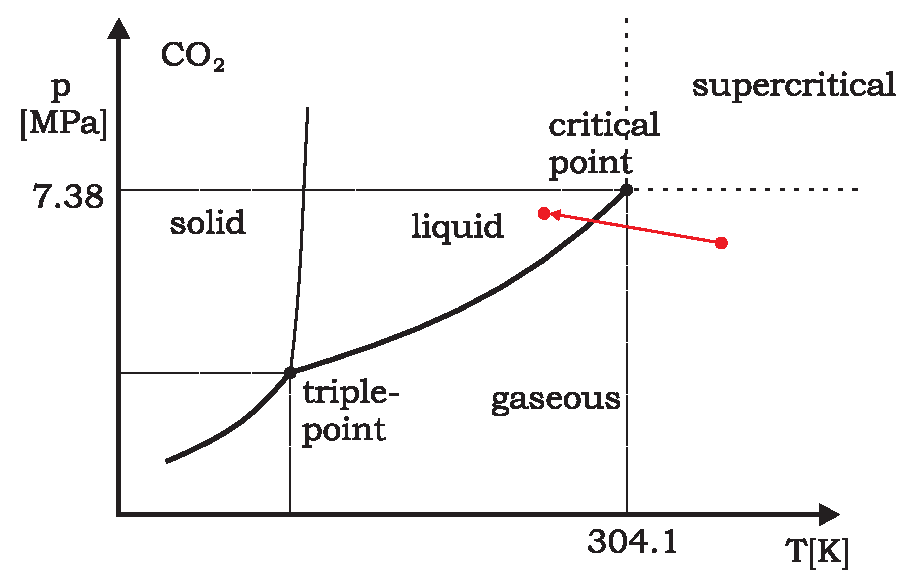
\includegraphics[width=0.9\textwidth]{figures/phase-diagram-co2.eps}
\caption{Phase diagram of carbon dioxide. The two extreme conditions ($\unit[400]{K}$ at $\unit[6.5]{MPa}$ and $\unit[300]{K}$ at $\unit[7]{MPa}$) are crossing a phase boundary of \co2, so a phase change from hot gas to  to liquid state will be forced.}
\label{fig-eos-phase}
\end{figure}

%
\begin{table}[htbp]
\caption{References for fluid properties of \ch4, \co2, \h2o, and \n2}
%\centering
\label{tab-eos-fluid_prop_bm}
\begin{center} 	
\begin{tabular}{llll}
\toprule
\textbf{Fluid} 	& \textbf{Specifier}   & \textbf{Density} 	& \textbf{Viscosity}  \\
\midrule
Methane \ch4			& CH4-RK     			&  \cite{RedKwo:49} & Friend, 1989 \cite{FriElyIng:89}\\
            			& CH4-PR     			&  \cite{PenRob:75} &    \\
             			& CH4-HE    			&  \cite{SetWag:91} &    \\
\midrule
Carbon dioxide \co2 	& CO2-RK     			&  \cite{RedKwo:49}  & Fenghour, 1998 \cite{FenWakVes:98} \\
                    	& CO2-PR     			&  \cite{PenRob:75}  &    \\
                   		& CO2-HE     			&  \cite{SpaWag:96}  &    \\
\midrule
Water \h2o 				& H2O-RK     			&  \cite{RedKwo:49}  & IAPWS, 1998 \cite{IAPWS:08a}      \\ 
           				& H2O-PR     			&  \cite{PenRob:75}  &    \\
           				& H2O-HE     			&  \cite{WagPru:02}  &    \\
\midrule
Nitrogen \n2 			& N2-RK      			& \cite{RedKwo:49}   & Stephan, 1987 \cite{SteKraLae:87} \\
             			& N2-PR     			&  \cite{PenRob:75}  &    \\
             			& N2-HE     			&  \cite{SpaLem:00}  &    \\
\bottomrule
\end{tabular}
\end{center}
\end{table}

%% \newfont{\tensy}{cmsy10}
%% \newcommand{\chemical}[1]{{$\fontdiment16\tensy=3.0pt\fontdiment17\tensy=3.0pt \mathrm{#1}$}}


%\subsection{Thermodynamic properties}

\subsection{Density} \label{eos-density}

In subterranean oil and gas reservoirs, properties of gases and liquids strongly depend from environmental pressure and temperature conditions. Equations of state (EOS) may be used to describe the relationship of volume, pressure and temperature of a real fluid. The knowledge of a fluids volume or its density is essential to estimate further thermodynamic properties. The first EOS for real gases, which was based on the ideal gas law, was presented by Johannes Diderik \textsc{van der Waals} in 1873 \cite{VanWaa:73}. In 1910 he received the Nobel prize for the development of the equation

\begin{equation}
p=\frac{RT}{V_m-b}-\frac{a}{V^2_m}
\label{eq-van-der-waals}
\end{equation}

where $p$ is the pressure, $R$ is the gas constant, $T$ is the temperature, $V_m$ is the molare volume and $a$ and $b$ are correcting parameters. 

%For the development of this equation \eqref{eq-van-der-waals}, \textsc{van der Waals} received the Nobel prize in 1910.
%
%\begin{equation}
%P=\frac{RT}{v-b}-\frac{a}{v^2}
%\label{eq-van-der-waals}
%\end{equation}

%In the current version of GeoSys\,(4.10.0), three different Equations of state are implemented. 
%\begin{itemize}
%	\item \textsc{Redlich-Kwong}, 1949 \cite{RedKwo:49}
%	\item \textsc{Peng-Robinson}, 1975 \cite{PenRob:75}
%	\item Fundamental equations, see \cite{SpaWag:96},\cite{PruWag:95},\cite{BueWag:06},  \cite{SpaLem:00}, and \cite{SetWag:91}
%\end{itemize}

Following three different EOS will be described, which are implemented in version GeoSys\,(4.10.00), based on the \textsc{van der Waals}-equation~\eqref{eq-van-der-waals}. % JG Satzumstellung

\paragraph{Redlich-Kwong equation of state (RKEOS)}
The Equation of \textsc{Redlich} and \textsc{Kwong} from 1949 \eqref{eq-rkeos1} represents just a little improvement of the van der Waals equation \cite{RedKwo:49}. It is given as 														

\begin{equation}
p=\frac{RT}{V_m-b}-\frac{a}{T^{0.5}\,V_m\,(V_m+b)}.
\label{eq-rkeos1}
\end{equation}

Its results are satisfactory only for temperatures above the critical point (see Tab.~\ref{tab-eos2}). 

\begin{table}[H]
  \caption{\label{tab-eos2}Fluid properties used in equations of state, where $\omega$ is the acentric factor, $T_c$ and $p_c$ are temperature und pressure at the critical point and $R$ ist the gas constant.}
  \begin{center}
\begin{tabular}{lrrrr}
\toprule
  substance 		& $\omega$ [-]  & $T_c$ [K] & $p_c$ [MPa] & $R$ [J/kg/K]\\
\midrule
  Carbon dioxide & 0.239  			& 304.13 & 7.38 		& 188.9\\
  Ethane         & 0.099  			& 305.32	& 4.87 		& 276.5\\
  Methane        & 0.011  			& 190.56 & 4.60 		& 518.3\\
  Water          & 0.344  			& 647.10 & 22.06 		& 461.5\\
\bottomrule
\end{tabular}
\end{center}
\end{table}

Equation \eqref{eq-rkeos1} can be recasted as a cubic equation in terms of volume

\begin{equation}
V_m^3-\frac{RT}{p}V_m^2-\left(\frac{RTb}{p}-\frac{a}{T^{0.5}p}+b^2\right)V_m-\frac{ab}{T^{0.5}p}=0.
\label{eq-rkeos2}
\end{equation}
              
This equation yields to one or three real roots depending on the number of phases in the system. In the two-phase region, the largest positive root represents the molar volume of the gas phase while the smallest root correspondes to the volume of the liquid phase. The correcting terms $a$ and $b$ are given as
													
\begin{equation}
a=0.4275\,\frac{R^2 T_c^{2.5}}{p_c}
\label{eq-rkeos_a}
\end{equation}

and

\begin{equation}
b= 0.0866\,\frac{RT_c}{p_c}
\label{eq-rkeos_b}
\end{equation}

where $T_c$ and $p_c$ are Temperature and pressure at the critical point (see Tab.~\ref{tab-eos2}). Figs.~\ref{fig-eos-dens-ch4-co2} and \ref{fig-eos-dens-h2o-n2} show the results of the RKEOS for several substances at four different temperatures in comparison to other equations of state.


%\begin{figure}
%\begin{minipage}{0.49\textwidth}
%\centering
%\includegraphics[width=1\textwidth]{FLUID_PROPERTIES/figures/dens-ch4.eps}
%\caption[bild1]{Density of $\mathrm{CH_4}$ derived by different equations of state}
%\label{fig-eos-dens-ch4}
%\end{minipage}
%%
%\hspace{0.02\textwidth
%}
%\begin{minipage}{0.49\textwidth}
%\centering
%\includegraphics[width=1\textwidth]{FLUID_PROPERTIES/figures/dens-co2.eps}
%\caption[bild2]{Density of $\mathrm{CO_2}$ derived by different equations of state}
%\label{fig-eos-dens-co2}
%\end{minipage}
%\end{figure}


\begin{figure}
\subfigure[]{\label{fig-eos-dens-ch4}\includegraphics[width=0.5\textwidth]{FLUID_PROPERTIES/figures/dens-ch4.eps}}
\hfill
\subfigure[]{\label{fig-eos-dens-co2}\includegraphics[width=0.5\textwidth]{FLUID_PROPERTIES/figures/dens-co2.eps}}
\caption[]{\label{fig-eos-dens-ch4-co2}Density of \ch4~\subref{fig-eos-dens-ch4} and \co2~\subref{fig-eos-dens-co2} derived by different EOS. There stand 
\setlength{\unitlength}{1ex}
\begin{picture}(5,1)
\thicklines \put(0,0.5){\line(1,0){5}}
\end{picture}
for the \textsc{Helmholtz} Free Energy,
\begin{picture}(5,1)
\thicklines \multiput(0,0.5)(2,0){3}{\line(1,0){1}}
\end{picture}
for the PREOS and
\begin{picture}(5,1)
\thicklines \multiput(0,0.5)(2,0){3}{\line(1,0){1}}\multiput(1.4,0.5)(2,0){2}{\line(1,0){0.25}}
\end{picture}
for the RKEOS. The colours refer to different temperatures (\textcolor{blue}{blue} - $\unit[280]{K}$, \textcolor{violet}{violet} - $\unit[320]{K}$, \textcolor{purple}{pink} - $\unit[400]{K}$, \textcolor{red}{red} - $\unit[680]{K}$).}
\end{figure}




%\begin{figure}
%\begin{minipage}{0.49\textwidth}
%\centering
%\includegraphics[width=1\textwidth]{FLUID_PROPERTIES/figures/dens-h2o.eps}
%\caption[bild1]{Density of $\mathrm{H_2O}$ derived by different equations of state}
%\label{fig-eos-dens-h2o}
%\end{minipage}
%%
%\hspace{0.02\textwidth
%}
%\begin{minipage}{0.49\textwidth}
%\centering
%\includegraphics[width=1\textwidth]{FLUID_PROPERTIES/figures/dens-n2.eps}
%\caption[bild2]{Density of $\mathrm{N_2}$ derived by different equations of state}
%\label{fig-eos-dens-n2}
%\end{minipage}
%\end{figure}


\begin{figure}
\subfigure[]{\label{fig-eos-dens-h2o}\includegraphics[width=0.5\textwidth]{FLUID_PROPERTIES/figures/dens-h2o.eps}}
\hfill
\subfigure[]{\label{fig-eos-dens-n2}\includegraphics[width=0.5\textwidth]{FLUID_PROPERTIES/figures/dens-n2.eps}}
\caption[]{\label{fig-eos-dens-h2o-n2}Density of \h2o~\subref{fig-eos-dens-h2o} and \n2~\subref{fig-eos-dens-n2} derived by different EOS. There stand 
\setlength{\unitlength}{1ex}
\begin{picture}(5,1)
\thicklines \put(0,0.5){\line(1,0){5}}
\end{picture}
for the \textsc{Helmholtz} Free Energy,
\begin{picture}(5,1)
\thicklines \multiput(0,0.5)(2,0){3}{\line(1,0){1}}
\end{picture}
for the PREOS and
\begin{picture}(5,1)
\thicklines \multiput(0,0.5)(2,0){3}{\line(1,0){1}}\multiput(1.4,0.5)(2,0){2}{\line(1,0){0.25}}
\end{picture}
for the RKEOS. The colours refer to different temperatures (\textcolor{blue}{blue} - $\unit[280]{K}$, \textcolor{violet}{violet} - $\unit[320]{K}$, \textcolor{purple}{pink} - $\unit[400]{K}$, \textcolor{red}{red} - $\unit[680]{K}$).}
\end{figure}



\paragraph{Peng-Robinson equation of state (PREOS)}
D.\,Y.\,\textsc{Peng} and D.\,B.\,\textsc{Robinson} presented an improvement of the RKEOS in 1975 \cite{PenRob:75}. The proposed equation is also a two-constant van der Waals-Type equation and combines simplicity and accuracy. The PREOS is very simple to solve and gives satisfying results within the whole fluid redion of a gas. It is given in the form

\begin{equation}
p=\frac{RT}{V_m-b}-\frac{a(T_c)\cdot \alpha (T_r,\omega)}{V_m^2+2\cdot bV_m-b^2}
\label{eq-preos1}
\end{equation}

where $a$ and $b$ are correcting terms. They can be derived by %\eqref{eq-preosa} and \eqref{eq-preosb} 

\begin{equation} 
a(T_c) = 0.45724\,\frac{R^2T_{c}^{2}}{p_c}
\label{eq-preosa}
\end{equation}

and

\begin{equation} 
b(T_c) = 0.07780\,\frac{RT_c}{p_c}
\label{eq-preosb}
\end{equation}

for the particular fluids under specification of pressure and temperature at the critical point.
Parameter $\alpha(T_r,\omega)$ is a dimensionless function of reduced temperature $T_r$ and acentric factor $\omega$. It is given as

\begin{equation} 
\alpha = \left( 1+ \left(0.37464 + 1.54226\,\omega - 0.26992\,\omega^2\right)\left(1-T_r^{0.5}\right)\right)^2
\label{eq-preosalpha1}
\end{equation}

for $\omega\leq{0.49}$ and

\begin{equation} 
\alpha = \left( 1+ \left(0.379642 + \left(1.48503-\left(1.164423-1.016666\,\omega\right)\omega\right)\omega\right)\left(1-T_r^{0.5}\right)\right)^2
\label{eq-preosalpha2}
\end{equation}

for $\omega > 0.49$. 

Tab.~\ref{tab-eos2} shows acentric factors and critical parameters for different real gases. The resulting density distribution of the 
PREOS is shown in Figs.~\ref{fig-eos-dens-ch4-co2} and \ref{fig-eos-dens-h2o-n2} at four different temperatures. 

%-----> JG: Vorschlag fr diesen Abschnitt s.u.

%\paragraph {Fundamental equations}				
%For highly precise results it is necessary to adapt fundamental equations based on the free energy, see \eqref{eq-fhe1}. Many authors used this approach to develop EOS for different substances, e.\,g.\,:
%
%\begin{itemize}
%\item \textsc{Span\&Wagner} \cite{SpaWag:96}, \cite{Spa:93}, \cite{SpaLem:00} for carbon dioxide and for nitrogen,
%\item \textsc{Pru\&Wagner} \cite{PruWag:95}, \cite{WagPru:02} for water,
%\item \textsc{Bcker\&Wagner} \cite{BueWag:06} for ethane and
%\item \textsc{Setzmann\&Wagner} \cite{SetWag:91} for methane.
%\end{itemize}
%
%Equation \eqref{eq-fhe1} shows \textsc{Helmholtz} free energy in dependence from density $\rho$ and temperature $T$ in its dimensionless shape, where $\phi^{o}$ is an ideal gas part and $\phi^{r}$ represents a residual part. 
%
%\begin{equation}
%\frac{f(\rho,T)}{RT}=\phi(\delta,\tau)=\phi^{o}(\delta,\tau)+\phi^{r}(\delta,\tau)
%\label{eq-fhe1}
%\end{equation}
%where $\delta=\rho/\rho_c$ and $\tau=T_c/T$\footnote{$\rho_c$ and $T_c$ are density and temperature at the critical point, see table \ref{tab-eos2}}
%The fundamental equation (\ref{eq-fhe1}) according to \textsc{Wagner} et al. (\cite{SpaWag:96},\cite{PruWag:95},\cite{BueWag:06}, and \cite{SetWag:91}) is one of the most precise EOS at present. The Equation and its derivatives can be used to describe all thermodynamic properties of a pure substance depending on density and temperature. So, it is necessary to solve the relationship between density, pressure, and temperature (eq. \ref{eq-fhe-dens}) iteratevly.
%
%\begin{equation}
%\frac{p(\delta,\tau)}{\rho RT}=1+\delta \frac{\partial \phi^r}{\partial \delta}
%\label{eq-fhe-dens}
%\end{equation}
%
%For water, the equation became international standard for the IAPWS since 1995. Certainly, the equation is complicated to solve and requires long computing time. Therefore, in the current version of Geosys, it is possible to choose between an iterative solving algorithm and an interpolation of density values out of a database. 
%


\paragraph {Fundamental equations}			
For highly precise results it is necessary to adapt fundamental equations based on the free energy. The \textsc{Helmholtz} free energy is given as

\begin{equation}
\frac{f(\rho,T)}{RT}=\phi(\delta,\tau)=\phi^{o}(\delta,\tau)+\phi^{r}(\delta,\tau)
\label{eq-fhe1}
\end{equation}
in dependence from density $\rho$ and temperature $T$ in its dimensionless form. These dimensionless parts are given as the terms $\delta=\rho/\rho_c$ and $\tau=T_c/T$, whereas $\rho_c$ and $T_c$ are density and temperature at the critical point (see Tab.~\ref{tab-eos2}).  The \textsc{Helmholtz} free energy provides relations between density, temperature and all thermodynamic properties of a fluid, which are expressed in the parameter $\phi^{o}$ as the ideal gas part and $\phi^{r}$ as the residual part. For their derivatives in the short forms like
$\phi^r_\delta$,\hspace{0.1cm} 
$\phi^r_{\delta\delta}$,\hspace{0.1cm} 
$\phi^r_\tau$,\hspace{0.1cm} 
$\phi^r_{\tau\tau}$,\hspace{0.1cm} 
$\phi^r_{\delta\tau}$,\hspace{0.1cm}
$\phi^o_\tau$,\hspace{0.1cm} 
$\phi^o_{\tau\tau}$
it is refered to \cite{SpaWag:96}.

Many authors used the approach of \textsc{Helmholtz} free energy to develop EOS for different substances, e.\,g.\,:

\begin{itemize}
\item \textsc{Span\&Wagner} \cite{SpaWag:96}, \cite{Spa:93}, \cite{SpaLem:00} for carbon dioxide and for nitrogen,
\item \textsc{Pruß\&Wagner} \cite{PruWag:95}, \cite{WagPru:02} for water,
\item \textsc{Bücker\&Wagner} \cite{BueWag:06} for ethane and
\item \textsc{Setzmann\&Wagner} \cite{SetWag:91} for methane.
\end{itemize}

The fundamental equation (\ref{eq-fhe1}) according to \textsc{Wagner} et al.\ (\cite{SpaWag:96},\cite{PruWag:95},\cite{BueWag:06}, and \cite{SetWag:91}) is one of the most precise EOS at present. The Equation and its derivatives can be used to describe all thermodynamic properties of a pure substance depending on density and temperature. So it is necessary to solve the relationship between density, pressure and temperature  iteratevly, as \eqref{eq-fhe-dens} shows

\begin{equation}
\frac{p(\delta,\tau)}{\rho RT}=1+\delta \frac{\partial \phi^r}{\partial \delta}.
\label{eq-fhe-dens}
\end{equation}

For water, the equation became international standard for the IAPWS\,\footnote{International Association for the Properties of Water and Steam} since 1995. Certainly, the equation is complicated to solve and requires long computing time. Therefore, in the version of GeoSys\,(4.10.00) it is possible to choose between an iterative solving algorithm 
and an interpolation of density values out of a database. 

The semi-empirical fundamental equation \eqref{eq-fhe1} has to be fitted to measurement data by computer algorithms for each substance. Depending on the fluid, there are up to 200 adjusting coefficients to ensure a very accurate fit to the real gas behaviour. For each 
substance, \eqref{eq-fhe1} has separate ranges of validity, which are shown in Tab.~\ref{tab-eos-val}.

\begin{table}[H]
  \caption{\label{tab-eos-val}Ranges of validity of the free \textsc{Helmholtz} equation \eqref{eq-fhe1} for serveral fluids valid from the melting point up to the indicated 
  values.}
 \begin{center}
 \begin{tabular}{lrrl}
  \toprule
  	substance		&$T$ [K]    &$p$ [MPa]	&reference\\
  \midrule
  Carbon dioxide 	& 216 		& 1100 		& \cite{SpaWag:96}, \cite{Spa:93}\\
  Nitrogen      	 & 1000 		& 2200 		& \cite{SpaLem:00}\\
  Ethane        	 & 520 		& 30 			& \cite{BueWag:06}\\ 
  Methane       	 & 625 		& 1000 		& \cite{SetWag:91}\\
  Water         	 & 1273 		& 1000 		& \cite{PruWag:95}, \cite{WagPru:02}\\
 \bottomrule
 \end{tabular}
 \end{center}
\end{table}

% The \textsc{Helmholtz} free energy provides relations between density, temperature and all thermodynamic properties of a fluid. Some of them are shown here: 
%
%$\phi^r_\delta = \left[\frac{\partial\phi^r}{\partial\delta}\right]_\tau$, $\phi^r_\delta\delta = \left[\frac{\partial^2\phi^r}{\partial\delta^2}\right]_\tau$, 
%$\phi^r_\tau = \left[\frac{\partial\phi^r}{\partial\tau}\right]_\delta$, $\phi^r_\tau\tau = \left[\frac{\partial^2\phi^r}{\partial\tau^2}\right]_\delta$, 
%$\phi^r_\delta\tau = \left[\frac{\partial^2\phi^r}{\partial\delta\partial\tau}\right]$, $\phi^o_\tau = \left[\frac{\partial\phi^o}{\partial\tau}\right]_\delta$, 
%$\phi^o_\tau\tau = \left[\frac{\partial^2\phi^o}{\partial\tau^2}\right]_\delta$.

%#####################################################################################################################
\subsection{Enthalpy}

The specific enthalpy $h$ is the whole amount of energy of a fluid. It consists of the internal energy and the volume changing work. It can be expressed by deviations of the free \textsc{Helmholtz} energy as

\begin{equation}
\frac{h(\delta,\tau)}{RT}=1+\tau\left(\phi^o_\tau+\phi^r_\tau\right)+\delta\phi^r_\delta.
\label{eq-fhe-enthalpy}
\end{equation}

%% \begin{figure}
%% \begin{minipage}{0.49\textwidth}
%% \centering
%% \includegraphics[width=1\textwidth]{FLUID_PROPERTIES/figures/enthalpy-co2.eps}
%% \caption[bild1]{Enthalpy of $\mathrm{CO_2}$ based on different equations of state}
%% \label{fig-eos-enthalpy-co2}
%% \end{minipage}
%% %
%% \hspace{0.02\textwidth}
%% %
%% \begin{minipage}{0.49\textwidth}
%% \centering
%% \includegraphics[width=1\textwidth]{FLUID_PROPERTIES/figures/entropy-co2.eps}
%% \caption[bild2]{Entropy of $\mathrm{CO_2}$ based on different equations of state}
%% \label{fig-eos-entropy-co2}
%% \end{minipage}
%% \end{figure}


%#####################################################################################################################
\subsection{Entropy}

The entropy $s$ represents which plenty of the energy of a system is potentially available to do work and which plenty of it is potentially defined as heat. In classical thermodynamics, the validity for the entropy is the thermodynamical system in equilibrium. The following equation is given for the entropy:

\begin{equation}
\frac{s(\delta,\tau)}{R}=\tau\left(\phi^o_\tau+\phi^r_\tau\right)-\phi^o-\phi^r.
\label{eq-fhe-entropy}
\end{equation}
%#####################################################################################################################
\subsection{Heat capacity}

The specific heat capacity of a fluid is defined as the amount of heat which is needed to increase the temperature of a fluid of $\unit[1]{kg}$ by $\unit[1]{K}$. In thermodynamics, it is distinguished between a heat capacity at constant pressure, the isobaric heat capacity, and a heat capacity at constant volume, the isochoric heat capacity. Both can be expressed in terms of free \textsc{Helmholtz} energy, like the following equations show:

\begin{itemize}
\item[]isobaric heat capacity
\end{itemize}
\begin{equation}
\frac{c_p(\delta,\tau)}{R}=-\tau^2\left(\phi^o_{\tau\tau}+\phi^r_{\tau\tau}\right)+\frac{\left(1+\delta\phi^r_\delta-\delta\tau\phi^r_{\delta\tau}\right)^2}{\left(1+2\delta\phi^r_\delta+\delta^2\phi^r_{\delta\delta}\right)} 
\label{eq-fhe-isobar}
\end{equation}

\begin{itemize}
\item[]isochoric heat capacity
\begin{equation}
\frac{c_v(\delta,\tau}{R}=-\tau^2\left(\phi^o_{\tau\tau}+\phi^r_{\tau\tau}\right).
\label{eq-fhe-isochor}
\end{equation}
\end{itemize}

%% \begin{figure}
%% \begin{minipage}{0.49\textwidth}
%% \centering
%% \includegraphics[width=1\textwidth]{FLUID_PROPERTIES/figures/isobar-co2.eps}
%% \caption[bild1]{Isobaric heat capacity of $\mathrm{CO_2}$ based on different equations of state}
%% \label{fig-eos-isobar-co2}
%% \end{minipage}
%% %
%% \hspace{0.02\textwidth}
%% %
%% \begin{minipage}{0.49\textwidth}
%% \centering
%% \includegraphics[width=1\textwidth]{FLUID_PROPERTIES/figures/isochor-co2.eps}
%% \caption[bild2]{Isochoric heat capacity of $\mathrm{CO_2}$ based on different equations of state}
%% \label{fig-eos-isochor-co2}
%% \end{minipage}
%% \end{figure}




%\begin{figure}%[ht]
%\begin{minipage}{0.49\textwidth}
%\centering
%\includegraphics[width=1\textwidth]{FLUID_PROPERTIES/figures/enthalpy-co2.eps}
%\caption[bild1]{Enthalpy of $\mathrm{CO_2}$ based on different equations of state}
%\label{fig-eos-enthalpy-co2}
%\end{minipage}
%%
%\hspace{0.02\textwidth}
%%
%\begin{minipage}{0.49\textwidth}
%\centering
%\includegraphics[width=1\textwidth]{FLUID_PROPERTIES/figures/entropy-co2.eps}
%\caption[bild2]{Entropy of $\mathrm{CO_2}$ based on different equations of state}
%\label{fig-eos-entropy-co2}
%\end{minipage}
%
%\vspace{2,5cm}
%%% \end{figure}
%%% 
%%% \begin{figure}[h]
%\begin{minipage}{0.49\textwidth}
%\centering
%\includegraphics[width=1\textwidth]{FLUID_PROPERTIES/figures/isobar-co2.eps}
%\caption[bild1]{Isobaric heat capacity of $\mathrm{CO_2}$ based on different equations of state}
%\label{fig-eos-isobar-co2}
%\end{minipage}
%%
%\hspace{0.02\textwidth}
%%
%\begin{minipage}{0.49\textwidth}
%\centering
%\includegraphics[width=1\textwidth]{FLUID_PROPERTIES/figures/isochor-co2.eps}
%\caption[bild2]{Isochoric heat capacity of $\mathrm{CO_2}$ based on different equations of state}
%\label{fig-eos-isochor-co2}
%\end{minipage}
%\end{figure}


\begin{figure}[t]
\subfigure[]{\label{fig-eos-enthalpy-co2}\includegraphics[width=0.5\textwidth]{FLUID_PROPERTIES/figures/enthalpy-co2.eps}}
\hfill
\subfigure[]{\label{fig-eos-entropy-co2}\includegraphics[width=0.5\textwidth]{FLUID_PROPERTIES/figures/entropy-co2.eps}}
\caption[]{\label{fig-eos-enthalpy-entropy-co2}Enthalpy~\subref{fig-eos-enthalpy-co2} and entropy~\subref{fig-eos-entropy-co2} of $\mathrm{CO_2}$ based on different EOS. There stand 
\setlength{\unitlength}{1ex}
\begin{picture}(5,1)
\thicklines \put(0,0.5){\line(1,0){5}}
\end{picture}
for the \textsc{Helmholtz} Free Energy,
\begin{picture}(5,1)
\thicklines \multiput(0,0.5)(2,0){3}{\line(1,0){1}}
\end{picture}
for the PREOS and
\begin{picture}(5,1)
\thicklines \multiput(0,0.5)(2,0){3}{\line(1,0){1}}\multiput(1.4,0.5)(2,0){2}{\line(1,0){0.25}}
\end{picture}
for the RKEOS. The colours refer to different temperatures (\textcolor{blue}{blue} - $\unit[280]{K}$, \textcolor{violet}{violet} - $\unit[320]{K}$, \textcolor{purple}{pink} - $\unit[400]{K}$, \textcolor{red}{red} - $\unit[680]{K}$).}
\end{figure}

\begin{figure}[h]
\subfigure[]{\label{fig-eos-isobar-co2}\includegraphics[width=0.5\textwidth]{FLUID_PROPERTIES/figures/isobar-co2.eps}}
\hfill
\subfigure[]{\label{fig-eos-isochor-co2}\includegraphics[width=0.5\textwidth]{FLUID_PROPERTIES/figures/isochor-co2.eps}}
\caption[]{\label{fig-eos-isobar-isochor-co2}Isobaric heat capacity~\subref{fig-eos-isobar-co2} and isochoric heat capacity~\subref{fig-eos-isochor-co2} of $\mathrm{CO_2}$ based on different EOS. There stand 
\setlength{\unitlength}{1ex}
\begin{picture}(5,1)
\thicklines \put(0,0.5){\line(1,0){5}}
\end{picture}
for the \textsc{Helmholtz} Free Energy,
\begin{picture}(5,1)
\thicklines \multiput(0,0.5)(2,0){3}{\line(1,0){1}}
\end{picture}
for the PREOS and
\begin{picture}(5,1)
\thicklines \multiput(0,0.5)(2,0){3}{\line(1,0){1}}\multiput(1.4,0.5)(2,0){2}{\line(1,0){0.25}}
\end{picture}
for the RKEOS. The colours refer to different temperatures (\textcolor{blue}{blue} - $\unit[280]{K}$, \textcolor{violet}{violet} - $\unit[320]{K}$, \textcolor{purple}{pink} - $\unit[400]{K}$, \textcolor{red}{red} - $\unit[680]{K}$).}
\end{figure}




Due to the high number of adjusting coefficients, the properties based on the \textsc{Helmholtz} free energy may be seen as very 
accurate. On the other hand, the iterative solution of \eqref{eq-fhe-dens} takes long computing times, so for long-term simulations or for simulations with a high number of elements, it would be better to use the \textsc{van der Waals}-type equations of \textsc{Redlich-Kwong} or \textsc{Peng-Robinson}. These cubic equations are easy to solve and lead to results very fast. Figs.~\ref{fig-eos-enthalpy-entropy-co2} and \ref{fig-eos-isobar-isochor-co2} illustrate, in which range of temperature and pressure those simple EOS may be used. Here, thermodynamical properties of carbon dioxide based on temperature and density are shown calculated by different EOS. In general, if temperature rises while pressure is declining, the behaviour of a fluid approaches to that of the ideal gas and the cubic equations of state give suitable results. For instance, the resulting entropy and enthalpy values of carbon dioxide at low pressures and high temperatures are identical, regardless of the density model they are based on (see Fig.~\ref{fig-eos-enthalpy-co2} and \ref{fig-eos-entropy-co2}). In the liquid and the dense supercritical region, the results based on different EOS diverge increasingly.


%% \begin{figure}[t]
%% \begin{minipage}{0.49\textwidth}
%% \centering
%% \includegraphics[width=1\textwidth]{FLUID_PROPERTIES/figures/enthalpy-co2.eps}
%% \caption[bild1]{Enthalpy of $\mathrm{CO_2}$ based on different equations of state}
%% \label{fig-eos-enthalpy-co2}
%% \end{minipage}
%% \hspace{0.02\textwidth}
%% \begin{minipage}{0.49\textwidth}
%% \centering
%% \includegraphics[width=1\textwidth]{FLUID_PROPERTIES/figures/entropy-co2.eps}
%% \caption[bild2]{Entropy of $\mathrm{CO_2}$ based on different equations of state}
%% \label{fig-eos-entropy-co2}
%% \end{minipage}
%% %\end{figure}
%% %\begin{figure}[h]
%% \begin{minipage}{0.49\textwidth}
%% \centering
%% \includegraphics[width=1\textwidth]{FLUID_PROPERTIES/figures/isobar-co2.eps}
%% \caption[bild1]{Isobaric heat capacity of $\mathrm{CO_2}$ based on different equations of state}
%% \label{fig-eos-isobar-co2}
%% \end{minipage}
%% \hspace{0.02\textwidth}
%% \begin{minipage}{0.49\textwidth}
%% \centering
%% \includegraphics[width=1\textwidth]{FLUID_PROPERTIES/figures/isochor-co2.eps}
%% \caption[bild2]{Isochoric heat capacity of $\mathrm{CO_2}$ based on different equations of state}
%% \label{fig-eos-isochor-co2}
%% \end{minipage}
%% \end{figure}


In addition, in the vicinity of the saturation curve, the results based on the \textsc{van der Waals}-type EOS may show large variations compared to the fundamental equation based curves (\textsc{Helmholtz} free energy). Particularly, this becomes apparent from Figs.~\ref{fig-eos-isobar-co2} and \ref{fig-eos-isochor-co2}, where the heat capacities of $\mathrm{CO_2}$ are given. The heat capacities at $\unit[400]{K}$ and $\unit[680]{K}$ (in the supercritical region of $\mathrm{CO_2}$, where no phase boundary exists) are identical, independent from according density model. Within the two-phase region at $\unit[280]{K}$ and $\unit[320]{K}$, a strong deviation at the phase boundary can be seen.

For water, the cubic EOS are not suitable. Water is a high critical fluid, so its properties are to complex to be described by simple approaches. As we can see in Fig.~\ref{fig-eos-dens-h2o}, the RKEOS, as well as the PREOS equation give viable results only at pressures below $\unit[1]{MPa}$ and at high temperatures. Therefor it is recommended to use the fundamental equation of the \textsc{Helmholtz} free energy to estimate the density of water. 


       
%#####################################################################################################################			
%\subsection{Transport properties}
%\label{sec_TP}
%############################################################################################################################
\subsection {Viscosity} \label{sec-viscosity}
Many authors developed correlation equations for viscosity $\eta$ of fluids at a density $\rho$ and a temperature $T$. Those correlation equations may be composed of two or three terms, like

\begin{equation}
\eta (\rho,T) = \eta_{0} (T) + \eta_{ex} (\rho,T)
	\label{eq-two-term-visc}
\end{equation}

or

\begin{equation}
\eta (\rho,T) = \eta_{0} (T) + \Delta \eta (\rho,T) + \Delta \eta_c (\rho,T).
	\label{eq-three-term-visc}
\end{equation}


In the two-term form, the viscosity correlation consists of a zero-density limit viscosity $\eta_0(T)$ at a temperature $T$, and an excess contribution viscosity $\eta_{ex}(\rho,T)$ at a density $\rho$ and a temperature $T$. This type of correlation function is used (among others) by \textsc{Friend} et al.\ \cite{FriElyIng:89} or \textsc{Stephan} et al.\ \cite{SteKraLae:87}. The formulation can be enhaced by a term describing the viscosity in the immediate vicinity of the critical point, $\Delta \eta (\rho,T)$ \eqref{eq-three-term-visc}, as described in \textsc{Fenghour} et al.\ \cite{FenWakVes:98} or \textsc{Huber} et al.\ \cite{IAPWS:08a}. An overview about the used viscosity correlations for several substances is given in Tab.~\ref{tab-eos-visc}. To show an example, Fig.~\ref{fig-eos-visc-co2} portrays the resulting viscosities for carbon dioxide based on densities of different EOS.


\begin{table}[H]
  \caption{\label{tab-eos-visc}Ranges of $T$ and $p$ validity for viscosity correlations for several substances.}
  \begin{center}
  \begin{tabular}{lrrl}
  \toprule
  substance 		& $T$ [K]		& $p$ [MPa] 	& reference \\
  \midrule
  Carbon dioxide 	& 200--1500		& $\leq{300}$ 	& \cite{FenWakVes:98}\\
  Nitrogen       	& 70--1100		& $\leq{100}$ 	& \cite{SteKraLae:87}\\  
  Ethane         	& 90--625		& $\leq{30}$ 	& \cite{FriIngEly:91}\\ 
  Methane       	&	91--600		& $\leq{100}$	& \cite{FriElyIng:89}\\  
  Water          	& 273--1173		& $\leq{100}$	& \cite{IAPWS:08a}\\
  \bottomrule
 \end{tabular}
 \end{center}
\end{table}
  


%############################################################################################################################
\subsection {Thermal conductivity} \label{sec-thermal-conductivity}
%$~~$ \\
Similar to the correlations between viscosity and $T$ and $p$, the thermal conductivity $\lambda$ can be expressed by an equation consisting of the following three parts (see \cite{VesWak:90}): A conductivity in the limit of zero-density $\lambda^0(0,T)$, where only two-body interaction occurs, a term $\Delta_c\lambda (\rho,T)$ wich enhances the property function in the critical region of the fluid, and finally $\Delta\lambda (\rho,T)$ which represents the contribution of all other effects to the thermal conductivity at elevated densities including many-body collisions, molecular-velocity correlations and collisional transfer. This equation is

\begin{equation}
\lambda (\rho,T) = \lambda^0 (T) + \Delta\lambda (\rho)+ \Delta_c \lambda (\rho,T).
\label{EqEOS_visc}
\end{equation}

Fig.~\ref{fig-eos-hc-co2} shows the thermal conductivity of carbon dioxide at four temperatures based on different EOS. In Tab.~\ref{tab-eos-hc} the ranges for the validity of $T$ and $p$ concerning thermal conductivity correlations for several substances are shown.

\begin{table}[H]
 \caption{\label{tab-eos-hc}Ranges of $T$ and $p$ validity for thermal conductivity correlations for several substances.}
 \begin{center}
  \begin{tabular}{lrrl}
 \toprule
   substance 		& $T$ [K] 		& $p$ [MPa] 			& Reference \\
  \midrule
  Carbon dioxide 	& 200--1000		& $\leq{100}$ 			& \cite{FenWakVes:98}\\
  Nitrogen       	& 70--1100		& $\leq{100}$		 	& \cite{SteKraLae:87}\\  
  Ethane         	& $\leq{600}$	& $\leq{70}$		 	& \cite{YouEly:87}\\ 
  Methane       	& $\leq{200}$ 	& $\leq{600}$		 	& \cite{YouEly:87}\\  
  Water          	& $\leq{800}$ 	& $\leq{100}$		 	& \cite{IAPWS:08b}\\
  \bottomrule
 \end{tabular}
 \end{center}
\end{table}

%\begin{figure}
%\begin{minipage}{0.49\textwidth}
%\centering
%\includegraphics[width=1\textwidth]{FLUID_PROPERTIES/figures/viscosity-co2.eps}
%\caption[bild1]{Viscosity of $\mathrm{CO_2}$ based on different EOS}
%\label{fig-eos-visc-co2}
%\end{minipage}
%%
%\hspace{0.02\textwidth
%}
%\begin{minipage}{0.49\textwidth}
%\centering
%\includegraphics[width=1\textwidth]{FLUID_PROPERTIES/figures/heat-conductivity-co2.eps}
%\caption[bild2]{Thermal conductivity of $\mathrm{CO_2}$ based on different EOS}
%\label{fig-eos-hc-co2}
%\end{minipage}
%\end{figure}



\begin{figure}[t]
\subfigure[]{\label{fig-eos-visc-co2}\includegraphics[width=0.5\textwidth]{FLUID_PROPERTIES/figures/viscosity-co2.eps}}
\hfill
\subfigure[]{\label{fig-eos-hc-co2}\includegraphics[width=0.5\textwidth]{FLUID_PROPERTIES/figures/heat-conductivity-co2.eps}}
\caption[]{\label{fig-eos-visc-hc-co2}Viscosity~\subref{fig-eos-visc-co2} and thermal conductivity~\subref{fig-eos-hc-co2} of $\mathrm{CO_2}$ based on different EOS. There stand 
\setlength{\unitlength}{1ex}
\begin{picture}(5,1)
\thicklines \put(0,0.5){\line(1,0){5}}
\end{picture}
for the \textsc{Helmholtz} Free Energy,
\begin{picture}(5,1)
\thicklines \multiput(0,0.5)(2,0){3}{\line(1,0){1}}
\end{picture}
for the PREOS and
\begin{picture}(5,1)
\thicklines \multiput(0,0.5)(2,0){3}{\line(1,0){1}}\multiput(1.4,0.5)(2,0){2}{\line(1,0){0.25}}
\end{picture}
for the RKEOS. The colours refer to different temperatures (\textcolor{blue}{blue} - $\unit[280]{K}$, \textcolor{violet}{violet} - $\unit[320]{K}$, \textcolor{purple}{pink} - $\unit[400]{K}$, \textcolor{red}{red} - $\unit[680]{K}$).}
\end{figure}



%-------------------------------------------------------------------------
\newpage
\section{Mechanical properties}
\label{sec:m_properties}
%\section{Mechanical properties}
%\label{sec:m_properties}

Constitutive equations (i.e. constitutive relations, material laws) are relations between measures of deformation (e.g. strain tensor) and internal force density functions (stress tensor) resulting from the action of external forces. Usually, they are not laws of nature but represent mathematical models intended to characterize the typical material behavior based on physically reasonable assumptions (particularly consistent with the thermodynamic balance relations) and mathematically correct approaches.

\subsection{Effective stress principle}
\label{sec:effstress}

Following the statements given in section~\ref{sec:momentum_balance} the total Cauchy's stress tensor in porous media is decomposed in partial stresses referring to the participating phases (note the sign convention of positive fluid phase pressure $p^{\gamma}$, but negative compressive normal stress for the solid phase).
\begin{equation}
\miu{\sigma}{}{}\,=\,(1-n)\,\mio{\sigma}{s}{}\,-\,n
\left(\sum\limits_{\gamma}S^{\gamma}\,p^{\gamma}\right)\mathbf{I}
\label{eq:totalstress}
\end{equation}
Considering the effective stress principle, relation (\ref{eq:totalstress}) can be modified defining the effective solid stress $\mib{\sigma}{eff}{s}{}$ as well as the overall fluid pressure $p^{\gamma}$
\begin{eqnarray}
\miu{\sigma}{}{} & = & 
(1-n)\left[
\mio{\sigma}{s}{}\,+\,\left(\sum\limits_{\gamma}S^{\gamma}\,p^{\gamma}\right)\mathbf{I}
\right]
\,-\,\left(\sum\limits_{\gamma}S^{\gamma}\,p^{\gamma}\right)\mathbf{I} \nonumber \\
 & = &
\miu{\sigma}{\mathrm{eff}}{}{}
\,-\,\left(\sum\limits_{\gamma}S^{\gamma}\,p^{\gamma}\right)\mathbf{I}
\label{eq:effect_stress}
\end{eqnarray}
The effective solid stress is the total solid stress reduced by the excess pore liquid pressure, but referred to the domain of the overall porous medium. Consequently, its absolute value is lower than the intrinsic stress of the solid skeleton. Constitutive relations for the solid phase of porous media combine the solid skeleton deformation (in terms of the strain tensor) with the effective solid stress. Selected models are presented in the next paragraphs. As they are equally valid for single-phase solid materials as well as for the solid phase of porous media, the special notation of the effective stress tensor will be omitted without loss of generality.

Based on the stress decomposition (\ref{eq:effect_stress}), the equilibrium condition for the porous medium becomes
\begin{equation}
\rho \mio{g}{}{}
+
\,\nabla\,\cdot\,\miu{\sigma}{\mathrm{eff}}{}{}\,
-
\left(\sum\limits_{\gamma}S^{\gamma}\,p^{\gamma}\right)\mathbf{I}
=
\,\mathbf{0}
\label{eq:equi_mod}
\end{equation}

%---
\subsection{Material classes}
\label{sec:matclass}

Usually laboratory tests are performed on specimens to investigate the mechanical behavior. Within this context, similar stress-strain curves can be caused by different physical effects, e.g. a nonlinear stress-strain curve does not necessarily suggest inelastic material behavior. For the sake of clarity, it is possible to introduce a classification of materials based on some essential distinctly identifiable material phenomena. For instance, comparatively simple experiments can be performed to investigate if the stress-strain curves are rate-dependent, and if hysteresis phenomena occur indicating dissipative effects.

\begin{figure}[htb!]
\begin{center}
\footnotesize
\includegraphics[width=0.95\textwidth]{figures/matbehav_el_elpl.eps}
\caption{Experimentally observed rate-independent solid material behavior. Cyclic uniaxial stress-strain curves \cite{Haupt:2002}: elasticity (left) and elastoplasticity (right)}
\label{fig:matbehav_el_elpl}
\end{center}
\end{figure}
\begin{figure}[htb!]
\begin{center}
\footnotesize
\includegraphics[width=0.95\textwidth]{figures/matbehav_vel_vpl.eps}
\caption{Experimentally observed rate-dependent solid material behavior. Cyclic uniaxial stress-strain curves \cite{Haupt:2002}: viscoelasticity (left) and viscoplasticity (right)}
\label{fig:matbehav_vel_vpl}
\end{center}
\end{figure}

\newpage

Based on these assumptions the observable material behavior can be divided into four different basic classes:
\begin{itemize}
\item rate-independent without hysteresis,
\item rate-independent with hysteresis,
\item rate-dependent without hysteresis, and
\item rate-dependent with hysteresis.
\end{itemize}
Figs.~\ref{fig:matbehav_el_elpl} and \ref{fig:matbehav_vel_vpl} schematically show typical cyclic stress-strain curves for these material classes. The equlibrium curves, presented in Figs.~\ref{fig:matbehav_vel_vpl} can be observed as a result of relaxation experiments.

According to the experimental observations, there are four classes of mathematical models matching the material classes defined above:
\begin{itemize}
\item the theory of elasticity describes rate-independent material behavior without hysteresis,
\item the theory of (elasto)plasticity describes rate-independent material behavior with hysteresis,
\item the theory of viscoelasticity describes rate-dependent material behavior without hysteresis, and
\item the theory of viscoplasticity describes rate-dependent material behavior with hysteresis.
\end{itemize}

Physically significant constitutive relations in the uniaxial case can be defined for the four classes of material theories based on so-called rheological models. These complex models consist of a simple networks of individual rheological elements (cf. Fig.~\ref{fig:rheomod_elem}), like
\begin{itemize}
\item elastic springs, which correspond to the linear stress-strain relation
\begin{equation}
\sigma\,=\,k\,\varepsilon
\end{equation}
with the spring constant $k$ representing the proportionality factor,  
\item viscous dashpots, which represent Newtonian viscous substances, and obey a linear relation between stress and strain rate
\begin{equation}
\sigma\,=\,\eta\,\mathop{\varepsilon}\limits^{\miu{.}{}{}}
\end{equation}
with the proportionality factor $\eta$ characterizing the viscosity, and
\item Coulomb friction elements, resisiting any motion until a threshold stress $\sigma^{\star}$ is reached, whereas behind the threshold irreversible deformations occur
\begin{equation}
\varepsilon\,=\,
\left\{
\begin{array}{ll}
0,              & \qquad\mbox{if}\quad\sigma\,<\,\sigma^{\star}  \\[1.5ex]
\varepsilon(t), & \qquad\mbox{if}\quad\sigma\,\geq\,\sigma^{\star}
\end{array}
\right.
\end{equation}
\end{itemize}

\newpage

\begin{figure}[htb!]
\begin{center}
\footnotesize
\includegraphics[width=0.95\textwidth]{figures/rheomod_elements.eps}
\caption{Mathematical modeling of solid material behavior. Basic individual elements of rheological models \cite{JCZ:2007}: spring element (left), dashpot element (middle) and frictional element (right)}
\label{fig:rheomod_elem}
\end{center}
\end{figure}

Differential equations, which are defined based on an appropriate composition of rheological models are only in a few special cases suitable to describe material response to external loading observed in reality. They can rather serve for marking the physical significance of mathematical models within the context of material theories. In Figs.~\ref{fig:rheomod_el_elpl} and \ref{fig:rheomod_vel_vpl} typical rheological models are presented, which characterize the material behavior of the four material classes defined above.

\begin{figure}[htb!]
\begin{center}
\footnotesize
\includegraphics[width=0.95\textwidth]{figures/rheomod_el_elpl.eps}
\caption{Mathematical modeling of rate-independent solid material behavior. Cyclic uniaxial stress-strain curves \cite{Haupt:2002}: elasticity (spring element -- left) and elastoplasticity (spring and frictional elements -- right)}
\label{fig:rheomod_el_elpl}
\end{center}
\end{figure}

\begin{figure}[htb!]
\begin{center}
\footnotesize
\includegraphics[width=0.95\textwidth]{figures/rheomod_vel_vpl.eps}
\caption{Mathematical modeling of rate-dependent solid material behavior. Cyclic uniaxial stress-strain curves \cite{Haupt:2002}: viscoelasticity (spring and dashpot elements -- left) and viscoplasticity (spring, dashpot, and frictional elements -- right)}
\label{fig:rheomod_vel_vpl}
\end{center}
\end{figure}

In Tab.~\ref{tab:matclass} some typical technical as well as natural (including geological) materials are assigned to the generalized material classes considering their material behavior, which can be observed for characteristic application cases. Generally, the classification of the material behavior depends on the real loading regime (e.g. small or large strains), environmental conditions (e.g. temperature), and the time scale of the physical processes under consideration. Changing one or more of these conditions one and the same material can demonstrate different mechanical behavior. Basically, no materials are actually purely elastic over a wide range of stresses, temperature, and time. Otherwise, developing and using complex constitutive models, which include all observable phenomena is not advisable for practical reasons. Constitutive relations, rather, should represent idealized and simplified models according to the most dominating conditions appearing in the practical applications under consideration.

\renewcommand{\arraystretch}{1.25}
\begin{table}[htb!]
\caption{Generalized classes of solid material behavior, and selected, typical representatives}
\label{tab:matclass}
\begin{center}
%\begin{tabular}{|l||l|l|}
\begin{tabular}{|p{0.18\textwidth}||p{0.37\textwidth}|p{0.33\textwidth}|}
\hline
Material class & Technical/natural material & Geomaterial \\
\hline\hline
elasticity & metals at small strains, & igneous rocks                 \\
           & ceramics,                & (e.g. granite),               \\
           & bone,                    & hard sedimentary rocks        \\
           & most other materials at small strains & (e.g. sandstone) \\
\hline
elastoplasticity & metals at large strains & most soils,                        \\
                 &                         & soft sedimentary rocks (e.g. tuff) \\
\hline
viscoelasticity & rubber,                 & rock salt (halite) \\
                & glass,                  &                    \\
                & soft biological tissues &                    \\
\hline
viscoplasticity & polymers (plastics),       & clay soils, \\
                & wood,                      & clay stone  \\
                & bitumen,                   &             \\
                & metals at high temperature &             \\
\hline
\end{tabular}
\end{center}
\end{table}
\renewcommand{\arraystretch}{1.00}
%
\hfill
%-------------------------------------------------------------------------
\newpage
\subsection{Elasticity}
\label{sec:elasticity}

In a micromechanical point of view, elasticity is predominantly caused by the evolution of interatomic forces in response to the impact of
external forces. It can be observed for crystalline substances (where the atoms are established in regular structures) as well as for
amorphous materials (where the atoms compose irregular structures), and is characterized by reversibility of the deformation processes and
the absence of any hysteresis. Furthermore, it is assumed that the current stress state is uniquely defined by the current strain state,
and does not depend on the strain history. Consequently, within the context of the constitutive model, the stress tensor is a function of
the strain tensor, but it does not depend on the strain rate. 

The isothermal isotropic linear elastic material model 
\begin{equation}
\miu{\sigma}{}{}\,=\,2\mu\,\miu{\varepsilon}{}{}\,+\,\lambda\,\mathrm{tr}(\miu{\varepsilon}{}{})\,\mathbf{I}
\label{eq:hooke_isotherm}
\end{equation}
known as generalized Hooke's law is the simplest of all constititive models for solid material behavior. Instead of the so-called
Lam{\'{e}} constants $\mu$ and $\lambda$, Hooke's law is often represented in terms of other material parameters like the Young's modulus
(i.e. elastic modulus, coefficient of elasticity, modulus of elasticity et al.) $E$, the Poisson's ratio $\nu$, the shear modulus $G$, and
the bulk modulus $K$. Some useful relations between these parameters are as follows:
\begin{eqnarray*}
E & = & \mu\,\ttfrac{2\mu+3\lambda}{\mu+\lambda},\qquad
\nu\,=\,\ttfrac{\lambda}{2(\mu+\lambda)} \\[2.0ex]
\mu & = & \ttfrac{E}{2(1+\nu)},\qquad
\lambda\,=\,\ttfrac{\nu E}{(1+\nu)(1-2\nu)} \\[2.0ex]
G & = & \ttfrac{E}{2(1+\nu)}\,=\,\mu \\[2.0ex]
K & = & \ttfrac{E}{3(1-2\nu)}\,=\,\ttfrac{(\mu+\lambda)(2\mu+3\lambda)}{3}
\end{eqnarray*}
Thus, the coefficients of the consistent material matrix $d\miu{\sigma}{}{}/d\miu{\varepsilon}{}{}$, which is required for the numerical
simulation of mechanical material behavior can be representeed in case of linear elasticity straightforward.
\begin{equation}
\fourtens{C}
\equiv
{C}_{ijkl}\,=\,\frac{d\sigma_{ij}}{d\varepsilon_{kl}}\,=\,2\mu\,\delta_{ik}\,\delta_{jl}\,+\,\lambda\,\delta_{ij}\,\delta_{kl}
\end{equation}

If a coupling of mechanical and thermal processes occur (non-isothermal mechanical processes), in addition to the strain caused by the
impact of external forces a volumetric thermal strain can be observed, which usually is linearly related to
the temperature difference.
\begin{equation}
\miu{\varepsilon}{\mathrm{th}}{}\,=\,\alpha_T\,(T-T_0)\,\mathbf{I}
\end{equation}
Here, $\alpha_T$ denotes the linear thermal expansion coefficient, and $T_0$ the initial temperature. In small strain solid mechanics it is
common practice to consider additive decompositions of the overall strain tensor into several constitutive parts according to the observed
physical phenomena. Considering thermoelastic material behavior, the overall strain tensor consists of an elastic part and a thermal part.
\begin{equation}
\miu{\varepsilon}{}{}\,=\,\miu{\varepsilon}{\mathrm{el}}{}\,+\,\miu{\varepsilon}{\mathrm{th}}{}
\end{equation}
As Hooke's law (\ref{eq:hooke_isotherm}) has to be perceived as a constitutive model, which assigns the local stress state to local elastic
strains, a non-isothermal generalization can be defined easily. 
\begin{equation}
\miu{\sigma}{}{}\,=\,2\mu\,\miu{\varepsilon}{\mathrm{el}}{}\,+\,\lambda\,\mathrm{tr}(\miu{\varepsilon}{\mathrm{el}}{})\,\mathbf{I}
                \,=\,2\mu\,\miu{\varepsilon}{}{}\,+\,\lambda\,\mathrm{tr}(\miu{\varepsilon}{}{})\,\mathbf{I}
                \,-\,(2\mu+3\lambda)\,\miu{\varepsilon}{\mathrm{th}}{}
\label{eq:hooke_nonisotherm}
\end{equation}
A conclusion drawn from Hooke's law of linear elasticity is the specific representation of the equilibrium condition for a thermo-poro-elastic porous medium in case of small strains.
\begin{equation}
\nabla\,\cdot\,
\left(
\miu{\sigma}{\mathrm{eff}}{}{}(\miu{\varepsilon}{}{})\,-\,
\left(\sum\limits_{\gamma}S^{\gamma}\,p^{\gamma}\right)\mathbf{I}\,-\,
\frac{2\mu+3\lambda}{3}\,\alpha_T\,(T-T_0)\,\mathbf{I}
\right)
\,=\,\rho\,\mio{g}{}{}
\label{eq:equi_thermo_poro_elast}
\end{equation}

Although no materials are actually linearly elastic over a wide range of stresses, elastic constitutive models are often quite useful and
accurate in many practical applications, e.g. in rock mechanics. The elastic material parameters given in Tab.~\ref{tab:rockelastpar} for 
selected soils and rocks show the large variation of material parameters, which is typical for geomaterials. 

\renewcommand{\arraystretch}{1.25}
\begin{table}[htb!]
\caption{Elastic material parameters for selected geomaterials}
\label{tab:rockelastpar}
\begin{center}
%\begin{tabular}{|l||l|l|}
\begin{tabular}{|p{0.25\textwidth}||p{0.22\textwidth}|p{0.2\textwidth}|}
\hline
Material & Young's modulus [GPa] & Poisson's ratio \\
\hline\hline
Sand       & 0.03\dots 0.6 & 0.10\dots 0.40 \\
\hline
Clay       & 0.03\dots 0.3 & 0.12\dots 0.40\\
\hline\hline
Clay stone & \ \,3\dots 11   & 0.10\dots 0.27 \\
\hline
Salt rock  & 12\dots 42  & 0.09\dots 0.49 \\
\hline
Sandstone  & \ \,4\dots 19   & 0.12\dots 0.20 \\
\hline
Granite    & 17\dots 56  & 0.11\dots 0.27 \\
\hline
Basalt     & 31\dots 97  & 0.19\dots 0.30 \\
\hline
Limestone  & 13\dots 53  & 0.11\dots 0.40 \\
\hline
\end{tabular}
\end{center}
\end{table}
\renewcommand{\arraystretch}{1.00}

\subsection{Elastoplasticity}
\label{sec:elastoplast}

The phenomenon of plastic yielding can be mainly observed in crystalline solid materials. It is associated with the motion of defects
(so-called dislocations, discontinuities) of the regular atomic structure during deformation. Elastoplastic material behavior is
characterized by elastic material response at the beginning of the deformation process. If a critical stress (the so-called yield stress)
is reached, plastic flow occurs, whereas elastic material behavior can be observed again at the beginning of each unloading phase of a
cyclic loading process.

In case of elastic-perfectly plastic material behavior, the stresses remain unchanged during plastic flow keeping the yield stress value.
Usually, real materials show elastoplastic material behavior with hardening effects, which are distinguished by an increase of stresses
during plastic flow with much lower slope of the stress-strain curve compared to the elastic phases of the entire deformation process.
Elastoplastic material behavior with neglegible elastic share is called rigid plasticity (see Fig.~\ref{fig:plastcases}).

\begin{figure}[htb!]
\begin{center}
\footnotesize
\includegraphics[width=0.95\textwidth]{figures/plastcases.eps}
\caption{Schematic representation of material behavior exhibiting plastic yielding \cite{JCZ:2007}: elastic-plastic with
strain hardening (left), elastic-perfectly plastic (middle), and rigid-perfectly plastic (right)}
\label{fig:plastcases}
\end{center}
\end{figure}

During plastic flow a certain fraction of the strain energy is transformed into thermal energy or stored as internal energy due to a
remodeling of the microstructure. Therefore, analyzing cyclic elastoplastic processes rate-independent hystereses can be observed.
Additionally, plastic deformation processes prove themselves to be irreversible.

In terms of the mathematical modeling of elastoplasticity no explicit stress-strain relation can be defined (no biunique relationship
between these quantities exists) due to the hysteresis effects. Instead, a mathematically ascertainable functional relation can be created
between the stress rate and the elastic strain rate.
\begin{equation}
\miu{\sigma}{}{\dot}\,=\,\fourtens{C}\,\miu{\varepsilon}{\mathrm{el}}{\dot}
\label{eq:elplastmatlaw}
\end{equation}

As shown in the case of thermoelasticity, the overall strain tensor can be additively split into two constitutive parts: an elastic one
$\miu{\varepsilon}{\mathrm{el}}{}$ and the partial plastic strain tensor $\miu{\varepsilon}{\mathrm{pl}}{}$.
\begin{equation}
\miu{\varepsilon}{}{\dot}\,=\,\miu{\varepsilon}{\mathrm{el}}{\dot}\,+\,\miu{\varepsilon}{\mathrm{pl}}{\dot}
\label{eq:strainsplit_pl}
\end{equation}
Usually, the plastic yielding is mathematically characterized based on appropriately defined so-called yield conditions $\Phi_{\mathrm{pl}}(\miu{\sigma}{}{})$ (i.e. flow condition, yield criterion). A yield condition is a relationship among the coefficients of the stress tensor separating the elastic domain in the stress space (which represents the area inside the yield condition) from the region of plastic yielding. Within this context, the plastic strain rate tensor is defined as follows:
\begin{equation}
\miu{\varepsilon}{\mathrm{pl}}{\dot}\,=\,
\lambda_{\mathrm{pl}}\,\frac{\partial\Phi_{\mathrm{pl}}(\miu{\sigma}{}{})}{\partial\miu{\sigma}{}{}}
\label{eq:plaststrainrate}
\end{equation}
with the so-called plastic multiplier $\lambda_{\mathrm{pl}}$. Consequently, the constitutive relation (\ref{eq:elplastmatlaw}) can be
reformulated. 
\begin{equation}
\miu{\sigma}{}{\dot}\,=\,\fourtens{C}
\left(\miu{\varepsilon}{}{\dot}\,-\,
\lambda_{\mathrm{pl}}\,\frac{\partial\Phi_{\mathrm{pl}}(\miu{\sigma}{}{})}{\partial\miu{\sigma}{}{}}
\right)
\label{eq:elplastmatlawmod}
\end{equation}

It is generally accepted that plastic yielding is accompanied by incompressible (volume-preserving) deformation processes. Thus, yield
conditions are usually defined in terms of the deviatoric stress tensor.
\begin{equation}
\miu{\sigma}{d}{}\,=\,\miu{\sigma}{}{}\,-\,\frac{1}{3}\mathrm{tr}(\miu{\sigma}{}{})\,\mathbf{I}
\label{eq:devstress}
\end{equation}
One of the most widely-used and simplest models is known as von~Mises yield condition
\begin{equation}
\Phi_{\mathrm{pl}}(\miu{\sigma}{}{})\,=\,
\sqrt{\ttfrac{3}{2}\miu{\sigma}{d}{}\ccdot\miu{\sigma}{d}{}}\,-\,\sigma_0\,=\,0
\label{eq:mises}
\end{equation}
with the initial yield stress $\sigma_0$ and the second invariant of the stress deviator.
\begin{equation}
\miu{\sigma}{d}{}\ccdot\miu{\sigma}{d}{}\,=\,
(\sigma_d){}_{ij}(\sigma_d){}_{ij}\,=\,(\sigma){}_{ij}(\sigma){}_{ij}\,-\,
\frac{1}{3}\left(\sigma_{ij}\delta_{ij}\right)^2
\end{equation}
A generalization of the von~Mises yield condition is the Drucker-Prager model
with the material parameters $a$ and $b$.
\begin{equation}
\Phi_{\mathrm{pl}}(\miu{\sigma}{}{})\,=\,
\sqrt{\ttfrac{2}{3}\miu{\sigma}{d}{}\ccdot\miu{\sigma}{d}{}}\,-\,b\,\mathrm{tr}(\miu{\sigma}{}{})\,-\,a\,=\,0
\label{eq:drucker_prager}
\end{equation}

Within the context of the analysis of geomaterials, elastic-plastic material models play a certain role particularly for soils, whereas
their relevance in rock mechanics for subsurface studies is rather minor due to the hardly observable cyclic processes.

\subsection{Viscoelasticity}
\label{sec:viscoelast}

Viscoelasticity is a typical material property of amorphous substances, particularly polymeric materials. If a wide variety of individual
macromolecular chains exhibit elastic material behavior under external loading, networks of macromolecular chains are characterized by
internal friction causing rate-dependent effects. Additionally, during mechanical loading, a certain part of strain energy transforms into
heat, which is responsible for the existence of hysteresis effects. Relaxation (decrease of stress values at constant strain after
instantaneous loading) and retardation (creep -- increase of strain values at constant stress after instantaneous loading) are typical
mechanical phenomena for viscoelastic materials. Both, relaxation and creep, tend towards asymptotic values, which represent the
equilibrium elastic state. In the equilibrium state of viscoelastic materials (at sufficiently small loading rates) no hysteresis occurs.
As well no hysteresis is observed at very high loading rates. In this case, the viscoelastic material behavior can be approximated by
elastic models using instanteneous parameters.

In contrast to elastoplastic materials, viscoelastic dissipative hysteresis effects are not necessarily accompanied by irreversible
deformation processes. A certain heat supply and/or a sufficiently long recovery period can reestablish the shape of a viscoelastic body
after mechanical loading.

There exists a wide variety of viscoelastic material models in terms of integral equations or differential relations. A large number of
them represent the generalization and modification of uniaxial approaches, which are based on more or less complex rheological models. The
simplest viscoelastic rheological models consist of one spring and one dashpot element, respectively (see Fig.~\ref{fig:rheomod_vel}).
\begin{figure}[htb!]
\begin{center}
\footnotesize
\includegraphics[width=0.95\textwidth]{figures/rheomod_vel.eps}
\caption{Mathematical modeling of reversible rate-dependent solid material behavior. Different combinations of a spring element with a
dashpot element \cite{JCZ:2007}: Kelvin-Voigt model (left) and Maxwell model (right)}
\label{fig:rheomod_vel}
\end{center}
\end{figure}

\newpage

The parallel connection of the spring and the dashpot elements is known as Kelvin-Voigt model. It is characterized by equal displacements
(and therefore equal strain values) in both of the individual elements, whereas the stress value of the model will be the sum of the
stresses in the spring and the dashpot. The constitutive behavior of the Kelvin-Voigt model is described by a differential equation.
\begin{equation}
\sigma\,=\,k\,\varepsilon\,+\,\eta\,\mathop{\varepsilon}\limits^{\miu{.}{}{}}
\label{eq:kelvin}
\end{equation}
If a stress $\sigma_0$ is instantaneously applied to a Kelvin-Voigt model, which is held constant thereafter, the solution of the
differential equation (\ref{eq:kelvin}) is given as follows:
\begin{equation}
\varepsilon\,=\,\frac{\sigma_0}{k}\,\left[1\,-\,\mathrm{e}^{-kt/\eta}\right]
\end{equation}
which indicates that the strain increases asymptotically to its steady-state (elastic) value $\sigma_0/k$. Thus, the Kelvin-Voigt model
represents the typical strain retardation, but neglecting any instantaneous strain.

The series connection of the spring and the dashpot elements is known as Maxwell model. Within this context, equal stress values occur in
both of the individual elements, whereas the total displacement (and therefore the strain) of the model will be the sum of the
displacements in the spring and the dashpot. The constitutive behavior of the Maxwell model can again be described by a differential
equation. 
\begin{equation}
\mathop{\varepsilon}\limits^{\miu{.}{}{}}\,=\,\frac{1}{\eta}\,\sigma\,+\,\frac{1}{k}\,\mathop{\sigma}\limits^{\miu{.}{}{}}
\label{eq:maxwell}
\end{equation}
Applying an instantaneous stress, a Maxwell element exhibits an instantaneous elastic response characterized by the spring constant $k$,
and a long-term viscous response specified by the viscosity $\eta$. If the Maxwell substance is subjected to an instantaneous jump in
strain with the amplitude $\varepsilon_0$, which is held constant thereafter, the differential equation (\ref{eq:maxwell}) can be solved closely.
The solution
\begin{equation}
\sigma\,=\,k\,\varepsilon_0\,\mathrm{e}^{-kt/\eta}
\end{equation}
indicates a stress decrease (relaxation) at constant (non-zero) strain, whereas in case of the Maxwell model the stress relaxes to zero,
simulating the behavior of a viscoelastic fluid.

\subsection{Viscoplasticity}
\label{sec:viscoplast}

Viscoplasticity is the most general material class, and the constitutive theories of viscoplasticity must be defined, on principle, to model all macroscopically observable phenomena of material behavior. The viscoplastic material class combines elements of all the other classes presented above. Micromechanical phenomena causing viscoplastic material behavior are exceptionally complex. 

Here, we will focus only on one typical effect of viscoplastic material behavior particularly relevant for geomaterials -- creep processes. Although in both cases characterizing the strain evolution at constant stress, viscoplastic creep differs from the viscoelastic creep (retardation) mentioned above, because no asymptotical strain value will be reached in the viscoplastic case. A typical viscoplastic creep curve is shown in Fig.~\ref{fig:creep}.

\begin{figure}[htb!]
\begin{center}
\footnotesize
\includegraphics[width=0.5\textwidth]{figures/creep.eps}
\caption{Schematical representation of a viscoplastic creep curve showing the three typical periods: primary, secondary, and tertiary creep \cite{JCZ:2007}. The three periods are indicated by the Roman numerals I, II and III, the point $A$ indicates the instantaneous elastic strain}
\label{fig:creep}
\end{center}
\end{figure}

For the viscoplastic creep behavior, generally, three typical periods can be observed. Whereas at all creep periods strain increases without reaching any asymptotical value, they differ in the strain rate. The first period, called primary creep, is characterized by a decreasing creep rate (transient creep), while for the second creep period, called secondary creep, a constant strain rate is observed (stationary creep, steady-state creep). The period of more or less constant strain rate is followed by the tertiary creep with ever-inreasing strain rate, eventually causing mechanical failure of the structure under consideration. The total reduction of the applied stresses results in a strain relaxation. Unloading in the primary creep period is characterized by a complete strain relaxation (similar to viscoelatic behavior). However, if stress is removed during the secondary creep period, residual strains remain (effect of plasticity).

Comparable to theory of elastoplasticity, as starting point for the constitutive modeling of viscoplastic stress-strain states serves the functional relation between the stress rate and the elastic strain rate (\ref{eq:elplastmatlaw}). The overall strain tensor is additively decomposed into several constitutive parts: apart from the partial elastic and plastic strain tensors a creep strain tensor is introduced $\miu{\varepsilon}{\mathrm{c}}{}$.
\begin{equation}
\miu{\varepsilon}{}{\dot}\,=\,\miu{\varepsilon}{\mathrm{el}}{\dot}\,+\,\miu{\varepsilon}{\mathrm{pl}}{\dot}\,+\,\miu{\varepsilon}{\mathrm{c}}{\dot}
\label{eq:strainsplit_vpl}
\end{equation}
Similar to the plastic potential (yield condition), the creep behavior is mathematically characterized based on appropriately defined creep potentials $\Phi_{\mathrm{c}}(\miu{\sigma}{}{})$ representing, again, relationships among the coefficients of the stress tensor. Consequently, the creep strain rate tensor is defined as follows:
\begin{equation}
\miu{\varepsilon}{\mathrm{c}}{\dot}\,=\,
\lambda_{\mathrm{c}}\,\frac{\partial\Phi_{\mathrm{c}}(\miu{\sigma}{}{})}{\partial\miu{\sigma}{}{}}
\label{eq:creepstrainrate}
\end{equation}
with the so-called creep multiplier $\lambda_{\mathrm{c}}$. Consequently, the constitutive relation (\ref{eq:elplastmatlaw}) can be
reformulated. 
\begin{equation}
\miu{\sigma}{}{\dot}\,=\,\fourtens{C}
\left(\miu{\varepsilon}{}{\dot}\,-\,
\lambda_{\mathrm{pl}}\,\frac{\partial\Phi_{\mathrm{pl}}(\miu{\sigma}{}{})}{\partial\miu{\sigma}{}{}}
\,-\,
\lambda_{\mathrm{c}}\,\frac{\partial\Phi_{\mathrm{c}}(\miu{\sigma}{}{})}{\partial\miu{\sigma}{}{}}
\right)
\label{eq:vplastmatlawmod}
\end{equation}

In geomechanics, the long-term rock behavior during the stationary creep period is the main focus of interest. One widely-used creep potential characterizing secondary creep is the so-called Norton's model
\begin{equation}
\Phi_{\mathrm{c}}(\miu{\sigma}{}{})\,=\,
\frac{\alpha}{n+1}\,
\left(\sqrt{\ttfrac{3}{2}\miu{\sigma}{d}{}\ccdot\miu{\sigma}{d}{}}\right)^{n+1}
\label{eq:norton}
\end{equation}
with the material parameters $\alpha$ and $n$.

\vspace{4.0ex}
All of the constitutive models mentioned above are idealized approximations of the actual material behavior. The presented models are relatively simple, and allow to gain a first insight into the material theory of deformable solid substances. Some other aspects, which are relevant for rock mechanics analyzing material behavior could not be considered here, and are subject of further studies, like:
\begin{itemize}
\item Rate-dependent deformation processes in porous media are caused by the pore pressure diffusion through the solid skeleton at a finite rate, and intrinsic viscous properties of the matrix material. A separated experimental observation of theses effects is quite challenging with according consequences to the constitutive modeling.
\item Certain geomaterials show a layered structure (e.g. shale, sandstone). Consequently, material properties of these substances depend on the direction of the impact of external forces (known as anisotropic material behavior), which has to be considered in constitutive relations.
\item Damage and failure of rocks play an important role in real geoprocesses, and require an individual consideration.
\item The analysis of wave propagation (dynamic phenomena) in geomaterials is relevant for all kinds of seismic activities or seismic analyses.
\item The design of appropriate lab tests is essential for the fundamental characterization of the material behavior, and the calibration of constitutive models.
\end{itemize}

%-------------------------------------------------------------------------
\section{Porous medium properties}

We have considered the properties of fluid (section \ref{sec:fluid_properties}) and solid phases (section \ref{sec:m_properties}), respectively. Many of the properties of a porous medium can be determined based on the assumption of the local thermodynamic equillibrium allowing a superposition of phase related characteristics - except of the hydraulic properties for multiphase flow, which are discussed in this section in more detail. We restart with the different definitions of saturation.

\subsection{Saturation}

Saturation of a fluid phase $\gamma$ is defined as the volumetric fraction $\epsilon^\gamma$ related to the sum of all fluid phases volumetric fractions.
%
\begin{eqnarray}
S^\gamma =
\frac{\epsilon^\gamma}{\sum_{\gamma}\epsilon^\gamma}
\end{eqnarray}

The sum of saturations of all fluid phases must be equal to unity (section \ref{sec:mixtures}).
%
Effective saturation is defined as \cite{BroCor:64}
%
\begin{eqnarray}
S_{\mbox{\small eff}}^\gamma =
\frac{S^\gamma-S_r^\gamma}{1-S_r^\gamma}
\end{eqnarray}

Moisture content (volumetric water content) is defined as the
product of porosity and saturation.
\begin{eqnarray}
\theta^\gamma = n S^\gamma
\end{eqnarray}

Gravimetric water content is defined as
\begin{eqnarray}
\omega^\gamma
=
n S^\gamma
\frac{\rho_d^s}{\rho^\gamma}
\end{eqnarray}

Applying the chain rule, we can express saturation changes in
following way.
\begin{eqnarray}
dS^\gamma =
\frac{dS^\gamma}{dp^\gamma} dp^\gamma
\end{eqnarray}

The capillary pressure-saturation functions as well as the relations between relative permeability and saturation are substantial constitutive equations required for multiphase flow. Within this context, usually algebraic expressions are fit to the corresponding experimentally observed curves. Among the widely-used of these algebraic expressions are the Brooks-Corey \cite{BC:1964} and van Genuchten \cite{Van:80} relations. If both are realized within the scientific software code developed by the authors, the numerical results presented in this paper are based on Brooks-Corey's approach.

%---
\subsection{Capillary pressure and relative permeability}
\index{quantity - pressure capillary}

As a consequence of interfacial tension a discontinuity in fluid
pressure exists across the interface that separates two immiscible
fluids. The partial pressure difference between two phases is
denoted as capillary pressure, which is a function of saturation.
%
\begin{eqnarray}
p_c^{\alpha\beta} = p^\beta -
p^\alpha = f(S^\alpha)
\end{eqnarray}

In general, capillary pressure is the difference between partial
pressures of non-wetting and wetting phases.
\begin{eqnarray}
p_c = p^{nw} - p^w =
f(S^w) 
\label{eqn:capillary_pressure}
\end{eqnarray}

Capillary pressure is always positive: $p_c>0 ,
\forall S$. It is often assumed that air is at a constant
atmospheric pressure taken as zero $p^g=0$. This means,
the macroscopic pressure of water in the unsaturated zone is
always negative due to suction.
%
Capillary pressure must be measured for given soils and pairs of
fluids. In general, these experiments are conducted for
equilibrium conditions with no fluid in motion. Various authors
have proposed analytical functions for capillary pressure -
saturation - relationships. 

\begin{figure}[htb!]
\begin{center}
\includegraphics[width=0.43\columnwidth]{figures/HYSTER.EPS}
\caption{Capillary hysteresis \cite{Bea:72}, with
$S_{w} = S^w$, $S_{w0} =
S_r^w$, $S_{n} = S^{nw}$,
$S_{n0} = S_r^{nw}$ } 
\label{fig:hysteresis}
\end{center}
\end{figure}
%
\index{process - hysteresis capillary}

The capillary pressure/saturation relationships
differ for drainage and rewetting (imbibition) \cite{Mua:76}. This phenomenon is
called hysteresis (Fig. \ref{fig:hysteresis}). Reasons for capillary pressure hysteresis are:
(i) varying pore shape (ink-bottle effect), (ii) contact angle
hysteresis (raindrop effect), (iii) entrapment of non-wetting
fluids, (iv) swelling and shrinking of solid grains.

To introduce the concept of relative permeability we recall the
Darcy law for flow of multiple fluid phases through porous
media, equation (\ref{eqn:momentum_balance_fluid}).
Fig. \ref{fig:k_rel} shows an example of relative permeabilities for both wetting and non-wetting phases.

\begin{figure}[htb!]
\begin{center}
\includegraphics[width=0.45\columnwidth]{figures/K_REL.EPS}
\caption{Relative permeability functions \cite{Bea:72} with
$S_{w} = S^w$, $S_{w0} =
S_r^w$, $S_{n} = S^{nw}$,
$S_{n0} = S_r^{nw}$, $k_{rn} = k^{nw}$,
$k_{rw} = k^w$ } 
\label{fig:k_rel}
\end{center}
\end{figure}
%

We consider some of the most used models after van Genuchten, Haverkamp, Brooks-Corey.

%-------------------------------------------------------------------------------
\subsubsection*{van Genuchten model \cite{Van:80}}

The definitions of effective saturation, capillary pressure and relative permeability for the van Genuchten model are as follows
%
\begin{eqnarray}
S_{\mbox{\small eff}} = \frac{S^w - S_r^w}{1 -
S_r^w} = \left( 1 + (\alpha \, p_c)^n
\right)^m \qquad , \qquad p_c > 0
\end{eqnarray}
%
\begin{eqnarray}
p_c = \left\{
\begin{array}{ll}
0 & S^w >
S^w_{\mbox{\footnotesize max}}
\\
\frac{\rho^w g}{\alpha} (S_{\mbox{eff}}^{-1/m}-1)^{1/n} &
S_r^w < S^w <
S^w_{\mbox{\footnotesize max}}
\\
{p_c}_{\mbox{\footnotesize max}} & S^w <
S_r^w
\end{array}
\right.
\end{eqnarray}
%
with
\begin{eqnarray}
m = 1 - \frac{1}{n}
\end{eqnarray}
%
\begin{eqnarray}
\mathbf{k}_{\mbox{\small rel}}(h) 
= 
\frac{1-(\alpha h)^{n-2}\,[1+(\alpha h)^n]^{-m}}{[1+(\alpha h)^n]^{2m}}
\end{eqnarray}

Figs. \ref{fig:VanGenuhetenParameter} and \ref{fig:vG_krel} show the capillary pressure and relative permeability functions corresponding to the parameters given in Tab. \ref{tab:van_Genuchten}, respectively.

\begin{figure}[htb!]
\begin{center}
\includegraphics[width=0.7\columnwidth]{figures/VanGenuheten_P.eps}
\caption{Capillary pressure / saturation relationship (Tuebingen experiment
2005)} \label{fig:VanGenuhetenParameter}
\end{center}
\end{figure}
%

\begin{figure}[htb!]
\begin{center}
\includegraphics[width=0.6\columnwidth]{figures/VanGenuheten_K.eps}
\caption{Relative permeability / saturation relationship (Tuebingen experiment
2005)} 
\label{fig:vG_krel}
\end{center}
\end{figure}

% Tabelle als Gleitumgebung
\begin{table}[htb!]
\caption{Model parameter}
\label{tab:van_Genuchten}
\begin{center}
\begin{tabular}{|l|l|l|l|}
\hline
$S_r^w$     & residual water saturation &  $ 0 $   &   \\
$S^w_{max}$ & maximal water saturation   & $0.645$ & $$ \\
$n$         & vG parameter  & $4.8$ &  \\
$\alpha$    & vG coefficient  & $320$ & $[m^{-1}]$ \\
\hline
\end{tabular}
\end{center}
\end{table}
%

%-------------------------------------------------------------------------------
\subsubsection*{Haverkamp model \cite{HavVauTouWieVac:77}}

The formulas for the Haverkamp model are given in terms of pressure head
$h=p^w/g\rho^w$\index{quantity - pressure head}
and moisture content
$\theta=nS^w$.\index{quantity - moisture content}
%
The definitions of effective saturation, capillary pressure and relative permeability for the Haverkamp model are as follows
%
\begin{eqnarray}
\theta = \frac{\alpha(\theta_s-\theta_r)}{\alpha+|h|^\beta} +
\theta_r
\end{eqnarray}
\begin{eqnarray}
h = \left( -\frac{\alpha}{\theta} (\theta - \theta_s + \theta_r)
\right)^{1/\beta}
\end{eqnarray}
%
\begin{eqnarray}
\mathbf{k}_{\mbox{\small rel}}(h) = K_s \frac{A}{A+|h|^\beta}
\end{eqnarray}

%
% Tabelle als Gleitumgebung
\begin{table}[htb!]
\caption{Model parameter}
\label{tab:Haverkamp}
\begin{center}
\begin{tabular}{|l|l|l|l|}
\hline
$\theta$    & volumetric water (moisture) content &         & $[cm^3/cm^3]$ \\
$\theta_r$  & residual volumetric water content   & $0.075$ & $[cm^3/cm^3]$ \\
$\theta_s$  & saturated volumetric water content  & $0.287$ & $[cm^3/cm^3]$ \\
$h(\theta)$ & soil water pressure head            &         & $[cm]$ \\
            & relative to the atmosphere          &         & \\
$\alpha$    &                                     & $1.611\times 10^6$ & $[Pa^{-1}]$ \\
$\beta$     &                                     & $3.96$ & \\
\hline
\end{tabular}
\end{center}
\end{table}
%

Fig. \ref{fig:Haverkamp} shows the capillary pressure saturation function corresponding to the parameters given in Tab. \ref{tab:Haverkamp}.

% *** EPS-Grafik ***
\begin{figure}[htb!]
\begin{center}
\footnotesize
%\psfrag{Synonym}[pos][pos]{Tex-Ersetzung}
%\psfrag{x}[][]{$t$}
%\psfrag{y}[b][t]{$y(t)$}
%\psfrag{t}[][]{ }
\includegraphics[width=0.95\columnwidth]{figures/haver1.eps}
\caption{Hydraulic properties of unsaturated soil
\cite{HavVauTouWieVac:77}} 
\label{fig:Haverkamp}
\end{center}
\end{figure}
%

%-------------------------------------------------------------------------------
\subsubsection*{Brooks \& Corey model \cite{BroCor:64}}

The Brooks-Corey equations relating the saturation to the capillary pressure are
\begin{equation}
p^c\,=\,p^D\,S_{\mathrm{eff}}^{-(1/\lambda)}
\qquad\mbox{for}\qquad p^c\geq p^D
\label{eq29}
\end{equation}
%\begin{equation}
%S_{\mathrm{eff}}\,=\,
%\left\{
%\begin{array}{ccl}
%1                                                            & , & \quad p^c\leq p^D \\[2.0ex]
%\left(\frac{\textstyle{p^D}}{\textstyle{p^c}}\right)^\lambda & , & \quad p^c > p^D
%\end{array}
%\right.
%\label{eq29}
%\end{equation}
where $p^D$ is usually known as entry pressure, $\lambda$ is a pore-size distribution index.
%
$S_{\mathrm{eff}}$ is a normalized wetting fluid saturation. For the case of \co2 as wetting fluid into a saline aquifer it is defined as
\begin{equation}
S_{\mathrm{eff}}=\frac{S^{l}-S^l_{\mathrm{res}}}{1-S^l_{\mathrm{res}}-S^{CO_2}_{\mathrm{res}}} \\
\label{eq30}
\end{equation}
where $S^l_{\mathrm{res}}$ is the wetting phase residual or irreducible saturation, and $S^{CO_2}_{\mathrm{res}}$ is the nonwetting phase residual saturation. The constitutive parameters $p^D$, $\lambda$, $S^l_{\mathrm{res}}$ and $S^{CO_2}_{\mathrm{res}}$ are identified by fitting Eq.~(\ref{eq29}) to experimental data. Within this context, the entry pressure is to be understood as the minimum pressure that the nonwetting fluid must have to enter the largest pores. The relations between the relative permeability and the saturation are given by
\begin{eqnarray}
k_{\mathrm{rel}}^{l} & = & \left(S_{\mathrm{eff}}\right)^{(2+3\lambda)/\lambda}
\label{eq31} \\[2.0ex]
k_{\mathrm{rel}}^{CO_2} & = & \left(1-S_{\mathrm{eff}}\right)^2\,\left(1-\left(S_{\mathrm{eff}}\right)^{(2+\lambda)/\lambda}\right)
\label{eq32}
\end{eqnarray}




%-------------------------------------------------------------------------
\chapter{Numerical methods}
\textit{by Wenqing Wang, Chan-Hee Park, Norihiro Watanabe and Olaf Kolditz}

The design, implementation and application of a concept for
object-orientated in finite element analysis of multi-field
problems is presented in this paper.
%
The basic idea of this concept is that the underlying governing
equations of porous media mechanics can be classified into
different types of partial differential equations (PDEs). In
principle, equal types of PDEs for diverse physical problems
differ only in material coefficients.
%
Local element matrices and vectors arising from the finite element
discretization of the PDEs are categorized into several types,
regardless of which physical problem they belong to (i.e. fluid flow, mass and
heat transport or deformation processes).
%
Element (ELE) objects are introduced to carry out the local
assembly of the algebraic equations. The object-orientation
includes a strict encapsulation of geometrical (GEO), topological
(MSH), process-related (FEM) data and methods of element objects.
%
Geometric entities of an element such as nodes, edges, faces and
 neighbors are abstracted into corresponding geometric element
objects (ELE-GEO). The relationships among these geometric
entities form the topology of element meshes (ELE-MSH).
%
Finite element objects (ELE-FEM) are presented for the local
element calculations, in which each classification type of the 
matrices and vectors is computed by a unique function. These
element functions are able to deal with different element types
(lines, triangles, quadrilaterals, tetrahedra, prisms, hexhedra) by 
automatically choosing the related element interpolation
functions.
%
For each process of a multi-field problem, only a single instance of 
the finite element object is required. The element objects provide a 
flexible coding environment for multi-field problems with different 
element types. Here, the C++ implementations of the objects are given and 
described in detail.
%
The efficiency of the new element objects is demonstrated by
several test cases dealing with thermo-hydro-mechanical (THM)
coupled problems for geotechnical applications.

\section{Introduction}

%\subsection{Motivation}
The numerical analysis of complex multi-field problems is an 
important issue for many engineering problems. A representative 
example is nuclear waste disposal. Nuclear waste repositories are 
constructed in deep geologic underground. Normally, the radioactive 
waste will generate heat for a long period of time with temperatures 
over 100$^\circ$C. Possibly, ground water \rev{flow} may be 
developed and gas will be produced due to the heating of the ground 
water. The coupling of thermal and hydraulic processes can cause 
mechanical damage in the near field of the host rock mass. To assess 
the safety of the underground repositories, the problem needs to be 
addressed as a thermo-hydro-mechanical
 (THM) coupled problem \cite{{LeSch:98},{deBoer:00},{deBoer:05},{StHuJi:02},{EhBl:02},{KolEtAl:2004a},{OKJO:04}}.
Although some commercial tools are already available, there is a 
tremendous demand in the development of fully coupled THM codes. 
Existing concepts couple obtainable codes which are specialized to 
hydraulic, mechanic or deformation problems. The coupling is then 
realized by data exchange between these codes. This procedure causes 
a rigorous restriction of the modeling of coupling phenomena. In 
this work we present a finite element class which can deal with 
thermal, hydraulic as well as mechanic problems.

%\subsection{Programming paradigms}
For the programming paradigms, there are two alternatives for finite 
element code design and development, i.e. procedure-oriented or 
object-oriented. The former does not encapsulate data and methods 
manipulating the data together, the latter does encapsulate data and 
methods and provides regulated communication between data and 
methods to perform tasks \cite{{StrB:00},{Budd:01}}. The object 
oriented paradigm \rev{facilitates} data abstract with its 
capabilities of data encapsulation, polymorphism and inheritance. 
Therefore, it provides us a easy way to develop and to maintain a 
code. This is a reason why more and more researchers are attracted 
to shift from using procedure oriented to  OOP paradigm in numerical 
analysis. Other reasons for its popularity is that software of 
increasing complexity has to be developed by permanently increasing 
programmer teams. OOP has significant advantages by allowing rapid 
software development through \rev{capsulation, inheritance and 
polymorph of data and methods}. 
%
The advantages of object-oriented programming for the development of 
engineering software was described in detail by \cite{Fen:90}.

%\subsection{History}
Although the fundamentals of object-orientated programming (OOP)
were established in the 1960s, it remains a very important concept
to face challenges in scientific computation, such as the solution
of coupled multi-field problems.
%
One of the first applications of the object-oriented paradigm to 
finite element analysis was published in 1990 \cite{FOFOST:90}, 
where essential components of finite element methods such as 
elements, nodes and materials were abstracted into classes. More 
efforts have been made by 
\cite{{FilDev:91},{Mack:92},{ZimYve:92},{YveZim:92}, 
{YveZim:93},{PidHud:93}, {RapKris:93}} in order to demonstrated the 
advantages of OOP over the procedure oriented programming. Moreover, 
the applications to many different physical problems have been 
investigated, such as linear stress analysis 
\cite{{ZimYve:92},{YveZim:92}, {YveZim:93}}, hypersonic shock waves 
\cite{BudPee:93}, structural dynamics \cite{PidHudli:93}, 2D Mises 
plasticity \cite{MenZim:93}, linear static problems 
\cite{{AdeFu:93},{AdeFu:95}}, electro-magnetics \cite{SilMes:94}, 
solidification process \cite{SaZa:99},  heat transfer as well as 
topological buildup \cite{RihKro94}. A process-oriented approach for 
the solution of multi-field problems in porous media is presented in 
\cite{{KolBau:04},{KolEtAl:2004a}}. Numerical objects for algebraic 
calculations in finite element analysis have been developed by 
\cite{{Scholz:92},{ZegHanAit:94},{LuWCD:95}}. \rev{In order to 
provide an automatic coding environment for finite element analysis, 
a symbolic code development concept is presented for the weak forms 
arising from the partial differential 
equations \cite{{ZimEyh:96},{EyhZim:96},{EyhZim:98},{EyhZim:01}}}.

Object design is the fundamental step in object-oriented
programming. The utilization of OOP to finite element analysis is
mainly focused on three aspects: (1) pre/post processing such as
mesh generation and graphical user interface, (2) linear algebra
and (3) finite element methods. In all these aspects, the core
object is the element object. The design of element objects is
associated with other objects corresponding to material
properties, numerical methods, local geometry and topology of
element etc. Specific material objects are described in the
most of references cited above.

In this part we present the design, implementation and application of 
object-orientation in finite element analysis for multi-physics 
problems. The development of a universal object for local 
finite element calculation and assembly is able to 
cope with different kinds of physical problems (i.e. different types 
of partial differential equations) and is, in particular, designed 
for strongly coupled problems. Additionally, object-orientation is used 
in description of mesh topology for the global assembly of system 
equations. The description of the programming semantics of these 
objects is given in C++. All the developments of this work are 
conducted within the framework of the scientific 
software project OGS \cite{geosys}. The the OO-FEM concept is verified by 
numerous test cases dealing with thermo-hydro-mechanical (THM) 
coupled problems in geotechnical as well as hydrological applications (Parts II and III of this book.)

\section{Object-orientation in finite element analysis}
\label{sec:ovl}

Almost all numerical methods eventually have to deal with the
solution of algebraic equation systems. The basic algorithms for
the discretization of partial differential equations (PDEs)
resulting from the initial-boundary-value-problems (IBVPs) of
continuum mechanics can be generalized in principle as follows:
time discretization, calculation of problem-specific node (finite
difference method - FDM), element (finite element method - FEM),
volume (finite volume method - FVM) contributions, incorporating
initial and boundary conditions, assembling and solving the resulting
equation system. For non-linear problems iteration schemes, such
as Picard or Newton methods, have to be used.

The general solution algorithm for the finite element method is
given in Table \ref{tab:alg1}.

\newpage

%.........................................................................
\rule{\textwidth}{0.25mm}
\begin{enumerate}
  \item Domain \rev{discretization} ( i.e. mesh generation): Creation of individual
geometric elements (e.g. triangles, tetrahedra) and their
topological relationships (mesh topology).
  \item Local element assembly: Depending on PDE type (section
\ref{sec:fem}) all element matrices and vectors have to be
computed. The element integration requires geometric operations
such as interpolation with shape functions, calculation of inverse
Jacobians and determinants. Additionally material functions have
to be computed in Gauss points. Material functions can depend on
field variables.
  \begin{itemize}
    \item Geometric element operations (shape functions, Jacobian),
    \item Material parameter calculation at Gauss points,
  \end{itemize}
  \item Global assembly of the algebraic equation $\mathbf{Ax=b}$: The local element
  entries are assembled into the global system matrix $\mathbf A$ and global
  RHS vector $\mathbf b$. The equations systems is established after \rev{incorporating} boundary conditions and source/sink terms.

  \begin{itemize}
    \item Assembly of system matrix $\mathbf A$ (including incorporation of boundary
    conditions),
    \item Assembly of RHS vector $\mathbf b$ (including incorporation of source/sink
    terms),
  \end{itemize}
  \item Solving the system equations,
  \item Iterative methods to handle non-linearities,
  \item Iterative methods to handle couplings (partitioned and monolithic schemes).
\end{enumerate}
\rule{\textwidth}{0.25mm}
\begin{table}[H]
\begin{tabular}{c}
\end{tabular}
 \caption{General solution procedure of the finite element method}
 \label{tab:alg1}
\end{table}

%.........................................................................
The implementation of the general solution algorithm for multi-field
IBVPs according to Table \ref{tab:alg1} is illustrated in Fig.
\ref{fig:alg}. The time loop represents time discretization. Within
the time loop, specified physical processes (e.g. flow, transport,
deformation) are solved using the finite element method (left box).
The solution procedure of each process is unique (middle box). The
basic part is the calculation and assembly of element contribution
(right box).

%.........................................................................
Based on above described general solution algorithm for
multi-field IBVPs, the fundamental concept of object-orientation
in finite element analysis is the generalization of
\begin{itemize}
    \item Process (PCS) types (section \ref{sec:pcs}),
    \item Equation (PDE) types (section \ref{sec:pde}),
    \item Element (ELE) types (section \ref{sec:ele}).
\end{itemize}

\begin{figure}[htb!]
\centering
\includegraphics[scale=0.45]{figures/algorithm.eps}
\caption{Implementation of solution algorithm} \label{fig:alg}
\end{figure}

%---
\subsection{Process (PCS) types}
\label{sec:pcs}

The central idea behind object-orientation of processes is that the
basic steps of the solution procedure: calculation of element
contributions, assembly of equation system (including treatment of
boundary conditions and source terms), solution of the equations
system, linearization methods and calculation of secondary variables, 
are independent of the specific problem (e.g. flow,
transport, deformation processes) \cite{{KolBau:04},{geosys}}. The
process (PCS) class provides basic methods in order to solve a PDE
in a very general way. The central part of the PCS object is the
member function \texttt{PCS::Execute()} (Fig. \ref{fig:alg}, middle
box) conducting these basic steps. Specific properties of the
mechanical problem, such as PDE type, primary and secondary
variables and material functions, are assigned during process
configuration (member function \texttt{PCS::Config()}). In order to
configure PCS instances we take advantage of polymorphism.

Fig. \ref{fig:pcs} illustrates the object-orientation of PCS types 
for the solution of IBVPs. The PCS object was designed to manage the 
complete solution algorithm in order to build the global equation 
system (EQS). In fact, the PCS object 'only' administrates 
references to geometric (GEO) objects (points, polylines, surfaces, 
volumes); MSH objects (mesh nodes, elements and mesh topology), 
node-related data such as initial (IC) and boundary (BC) conditions 
as well as source terms (ST); material data of porous media (fluid 
(MFP), solid (MSP), medium (MMP) and chemical (MCP) properties); 
parameters of the different numerical methods (NUM). PCS instances 
have 'only' pointers to the related objects as members. \rev{Objects 
IC, BC and ST have pointers to object GEO to specify geometrical 
entities, which are managed by PCS to find element nodes on them. 
The values in IC and BC and ST are assigned to element nodes found 
be their GEO members. Object GEO also play a key role in the  
 pre/post-process of the data of the finite element method.}

\begin{figure}[htb!]
\centering
\includegraphics[scale=0.5]{figures/pcs.eps}
\caption{Structure of the process (PCS) object} \label{fig:pcs}
\end{figure}

%-------------------------------------------------------------------------
\subsection{PDE types}
\label{sec:pde}

IBVPs in porous media mechanics, such as fluid flow, mass and heat 
transport, deformation can be categorized into elliptic, parabolic, 
hyperbolic or mixed equation types.

As an example to explain the generalization of PDE types, we
illustrate the treatment of Laplace terms, which appear in flow,
transport as well as deformation processes. In Fig. \ref{fig:lap}
the evaluation of finite element matrices for Laplace terms, i.e.
$\mathbb{D}\partial^2/\partial x^2$ is given, where $\mathbb{D}$ is 
a problem-specific material tensor. The special part of diffusion 
terms is the calculation of second order space derivatives. The 
second line of the equation in Fig. \ref{fig:lap} represents the 
  numerical integration of matrix being transformated into reference coordinates. From the view point of 
object-orientation we are faced with the following operations: 
tensor coordinate transformation ($\mathbf{T}$), Jacobian 
($\mathbf{J}$), integration ($\int$) and computation of material 
properties ($\mathbb D$, e.g. diffusivity, conductivity tensor). The latter is the only problem-specific.

\begin{eqnarray}
\mathbf K_e 
&=&
\int\limits_{\Omega_e} \nabla \Sh \mathbb{D}(\nabla\Sh)^{\mathrm{T}} d\Omega \\
&=& 
\sum\limits_{gp=1}\limits^{no\_gp} \int\limits_{\Omega_r} w_{gp} 
\left[
\nabla \Sh \mathbb{D}(\nabla \Sh)^{\mathrm{T}} \mathrm{det}\ \mathbf{J} 
\right]
\vert_{gp} d\Omega
\end{eqnarray}

\begin{figure}[htb!]
\centering
\shadowbox{
\begin{minipage}{0.95\textwidth}
%{\sffamily \raggedright \small
{\ttfamily \raggedright \small
void\ CFiniteElement::CalcLaplace()\\
\{\\
\ \ \textsl{//\ Loop\ over\ Gauss\ points}\\
\ \ \textbf{for}\ (gp\ =\ 0;\ gp\ $<${}\ no\_gp;\ gp++)\\
\ \ \{\\
\mbox{\ \ \ \ \ GaussData();\ \ \ \ \ \ \ \ \ \ \ \ \ \ \ \ \ \textsl{//\ Integration\ points\ and\ weights}}\\
\mbox{\ \ \ \ \ Jacobian();\ \ \ \ \ \ \ \ \ \ \ \  \ \ \ \ \ \ \textsl{//\ det\ $\mathbf{J}$,\ ${\mathbf J}^{-1}$}}\\
\ \ \ \ \ GradShapefct();\ \ \ \ \ \  \ \ \ \ \ \ \ \ \textsl{//\ $\nabla \Sh$}\\
\mbox{\ \ \ \ \ LaplaceMATFunction();\ \ \ \ \ \ \ \ \textsl{//\ Material\ parameters,\ $\mathbb{D}$}}\\
\mbox{\ \ \ \ \ \textbf{for}\ (i=0;\ i$<${}nnodes;\ i++)\ \ \ \ \textsl{//\ Loop\ over\ element\ nodes}}\\
\ \ \ \ \ \ \ \ \textbf{for}\ (j\ =\ 0;\ j\ $<${}\ nnodes;\ j++)\\
\ \ \ \ \ \ \ \ \ \{\\
\mbox{\ \ \ \ \ \ \ \ \ \ \ \ \textbf{if}(j$>${}i)\ \textbf{continue};\ \ \ \ \textsl{//\ Symmetry}}\\
\mbox{\ \ \ \ \ \ \ \ \ \ \ \ \textbf{for}\ (k\ =\ 0;\ k\ <{}\ ele\underline\ dim;\ k++)}\\
\mbox{\ \ \ \ \ \ \ \ \ \ \ \ \ \ \ \textbf{for}(l=0;\ l<{}ele\underline\ dim;\ l++)}\\
\mbox{\ \ \ \ \ \ \ \ \ \ \ \ \ \ \ \ \ \ ($\ast$Laplace)(i,j)\ +=\ fkt\ $\ast$\ dshapefct[k$\ast$nnodes+i]\ }\\
\mbox{\ \ \ \ \ \ \ \ \ \ \ \ \ \ \ \ \ \ \ \ \ \ \ \ \ \ \ \ \ \ \ \ \ \ \ \ $\ast$\ mat[ele\underline\ dim$\ast$k+l]\ }\\
\mbox{\ \ \ \ \ \ \ \ \ \ \ \ \ \ \ \ \ \ \ \ \ \ \ \ \ \ \ \ \ \ \ \ \ \ \ \ $\ast$\ dshapefct[l$\ast$nnodes+j];}\\
\ \ \ \ \ \ \ \ \ \}\\
\ \ \}\\
\}\\
\ \\
 }
\normalfont\normalsize


\end{minipage}
}
\caption{Finite element Laplace matrix and implementation}
\label{fig:lap}
\end{figure}

\begin{figure}[htb!]
\centering
\shadowbox{
\begin{minipage}{0.75\textwidth}
{\ttfamily \raggedright \small
void\ CFiniteElementPCS::LaplaceMATFunction()\\
\{\\
\ \ \textsl{//\ Calculate\ conductivity\ tensor\ $\mathbb D$ for\ Laplacian}\\
\ \ \ \textbf{switch}(PcsType)\{\\
\ \ \ \ \ \ \textbf{case}\ L:\ \textsl{//\ Liquid\ flow}\\
\ \ \ \ \ \ \textbf{case}\ U:\ \textsl{//\ Unconfined\ flow}\\
\ \ \ \ \ \ \textbf{case}\ G:\ \textsl{//\ Gas\ flow}\\
\ \ \ \ \ \ \textbf{case}\ T:\ \textsl{//\ Two-{}phase\ flow}\\
\ \ \ \ \ \ \textbf{case}\ C:\ \textsl{//\ Componental\ flow}\\
\ \ \ \ \ \ \textbf{case}\ H:\ \textsl{//\ Heat\ transport}\\
\ \ \ \ \ \ \textbf{case}\ M:\ \textsl{//\ Mass\ transport}\\
\ \ \ \ \ \ \textbf{case}\ O:\ \textsl{//\ Overland\ flow}\\
\ \ \ \ \ \ \textbf{case}\ R:\ \textsl{//\ Richard\ flow}\\
\ \ \ \}\\
\}\\
\ \\
 }
\normalfont\normalsize


\end{minipage}
}
\caption{Implementation of process dependent material functions}
\label{fig:mat1}
\end{figure}

Fig. \ref{fig:lap} shows the implementation of the Laplace term
calculation, in which $\Omega_r$ is the domain by the reference 
element. The \texttt{CalcLaplace()} member function of the finite 
element class works for different processes with different material 
functions (Fig. \ref{fig:mat1}) and geometric element types. A short 
description is given in the table below.

\small
\begin{tabular}{|l|l|}
  \hline
  % after \\: \hline or \cline{col1-col2} \cline{col3-col4} ...
  \texttt{Code} & Description \\
  \hline
  \texttt{gp} & Gauss integration points \\
  \texttt{GaussData()} & Calculation of Gauss weights \\
  \texttt{Jacobian()} & Calculation of Jacobian determinant and inverse \\
  \texttt{GradShapeFunction()} & Calculation of shape function derivatives \\
  \texttt{LaplaceMATFunction()} & Calculation of material coefficients \\
  \texttt{(*Laplace)(i,j)} & Finite element matrix \\
  \hline
\end{tabular}
\normalsize

%-------------------------------------------------------------------------
\subsection{Element (ELE) types}
\label{sec:ele}

The basic concept we apply is that: element data, such as geometrical and topological
properties, as well as operations of elements, such as
element matrix calculations and treatment of boundary conditions,
can be generalized.

The element object is the fundamental entity in both PDE and
element types. In Fig. \ref{fig:ele_concept} the structure of the
element object is illustrated. The element has two kinds of
properties connected geometry and PDE types.

\begin{figure}[H]
\centering
\includegraphics[scale=0.4]{figures/ele_concept.eps}
\caption{Structure of element object}
\label{fig:ele_concept}
\end{figure}

Element geometry includes the geometric type (line, triangle, quad, 
tetrahedron, prism, hexahedron), node coordinates, edges, faces and 
volume. Coordinate transformation functionalities are considered as 
geometric element properties. Element topology is defined by element 
neighbor relationships. Patch properties are available for finite 
volume approaches and flux calculations. The elements form the mesh 
topology. Different geometric element types can be combined (Fig. 
\ref{fig:ele_concept}) together to establish a mesh. Additionally, 
elements can be assigned to different meshes.
%%%% \cite{Kol:2005b}.

Depending on PDE type (elliptic, parabolic, hyperbolic, mixed),
different first or second order differential terms have to be
evaluated ($\partial/\partial t, \partial/\partial x,
\partial^2/\partial t^2, \partial^2/\partial x^2$). These differential
terms are categorized in corresponding FE matrix types (see section 
\ref{sec:fem}), mass matrix, Laplacian matrix, tangential matrix and 
coupling matrices. An obvious advantage of this element concept is 
that, depending on the geometric element type, interpolations (shape 
functions) and derivations as well as tensor operations and Gaussian 
integrations are conducted automatically in a correct way (see 
section \ref{sec:ele_fem}). For material tensor properties in 1D, 2D 
or 3D ($\mathbf{A,B,C,D(x)}$ in Fig. \ref{fig:ele_concept}), the 
correct matrix multiplications are conducted automatically. Material 
functions ($A,B,C,D(u)$ in Fig. \ref{fig:ele_concept}) are evaluated 
accordingly at corresponding Gaussian points of the selected 
element.

For the sake of object-orientation for numerical methods a so-called 
process (PCS) object was designed, implemented (\cite{KolBau:04}, 
section \ref{sec:pcs}) and successfully applied to different 
numerical methods (FEM: \cite{KolEtAl:2004a}, FDM: 
\cite{KolEtAl:2005a}, FVM: \cite{Bei:2005}).

%\providecommand{\sembrack}[1]{[\![#1]\!]}
\providecommand{\pD}[2]{\dfrac{\partial #1}{\partial #2}}
\providecommand{\oD}[2]{\dfrac{\mathrm d #1}{\mathrm d  #2}}
\providecommand{\abs}[1]{\lvert #1 \rvert}
%%\providecommand{\abs}[1]{\left\lvert #1 \right\rvert}
\providecommand{\norm}[1]{\left\lVert #1 \right\rVert}

\newcommand{\od}{\mathrm d}
%%%
\newcommand{\js}{\mathscr S}
%%%
%%material index
\newcommand{\pl}{\scriptscriptstyle \mathrm p}
\newcommand{\el}{\scriptscriptstyle \mathrm e}

%%Geometry
\newcommand{\Point}{ \bm x}

%%Displacement field
\newcommand{\Pressure}{p}
\newcommand{\Stress}{ \bm \sigma}
\newcommand{\inPStress}{ \Stress_{\imath}} %%% in-plane stress
\newcommand{\stress}{ \sigma}
\newcommand{\devStrs}{\bm s}
\newcommand{\Strain}{ \bm \epsilon}
\newcommand{\strain}{ \epsilon}
\newcommand{\Disp}{\mathbf u}
\newcommand{\disp}{u}
\newcommand{\vel}{\bf v}
\newcommand{\per}{\mathbf k}
\newcommand{\grv}{\mathbf g}
%%Plasticity
\newcommand{\yld}{ f}
\newcommand{\ppo}{ g}
\newcommand{\pHard}{\mathcal H}
\newcommand{\CT}{\mathbb C}
\newcommand{\DT}{\mathbb D}
\newcommand{\EM}{{\bm C}^{\el}}
\newcommand{\PM}{{\bm C}^{\pl}}
\newcommand{\EPM}{{\bm C}^{\el\pl}}
\newcommand{\mEM}{{\bm D}^{\el}}
\newcommand{\mPM}{{\bm D}^{\pl}}
\newcommand{\mEPM}{{\bm D}^{\el\pl}}
\newcommand{\rdl}{\dot \lambda}
\newcommand{\dl}{\lambda}
\newcommand{\dens}{\rho}

%%Flow
\newcommand{\densc}{\dens^{\gamma}}
\newcommand{\presc}{p^{\gamma}}
\newcommand{\pres}{p}
\newcommand{\sat}{S}
\newcommand{\Satc}{S^{\gamma}}
\newcommand{\RelK}{k^{\gamma}_{rel}}
\newcommand{\RelKa}{k_{rel}}
\newcommand{\poro}{n}
\newcommand{\Fluxf}{\mathbf{q}_{\scriptscriptstyle f}}
\newcommand{\Fluxv}{\mathbf{q}_{\scriptscriptstyle v}}
\providecommand{\perm}{ \mathbf k}
\newcommand{\asup}[2]{#1^#2}
\newcommand{\asub}[2]{#1_#2}
\newcommand{\supsub}[3]{{#1}^{#2}_{#3}}
\newcommand{\FlxDf}{\mathbf{J}}
\newcommand{\Sat}{S}
%%Heat
\newcommand{\HC}{C_p}
\newcommand{\Flux}{\mathbf{q}}

%%%FEM
\newcommand{\test}{w}
\newcommand{\Test}{\bm w}
\newcommand{\TestS}{\mathcal V}
\newcommand{\sh}{N}
% \newcommand{\Sh}{{\bm N}}

%%Math
\newcommand{\intD}{{\int}_{\Omega}}
\newcommand{\intB}{{\int}_{\Gamma}}
\newcommand{\dDom}{\,\mathrm{d} \Omega}
\newcommand{\dBdry}{\,\mathrm{d} \Gamma}
\newcommand{\nrl}{\mathbf n}
\newcommand{\tgl}{\mathbf t}
\newcommand{\I}{\mathbf I}

\section{General finite element formulations}
\label{sec:fem}

The method of weighted residuals is applied to derive the weak
formulation of the balance equations given in section
\ref{sec:balance_equations}.

Assume $\TestS^{\mathrm{n}}\subset
H^1_{\scriptscriptstyle{\Gamma}}(\Omega)^{\mathrm{n}}$ is the test
function space. For all $\test\in \TestS^{\mathrm{1}}$, we have
the weak form of the mass balance equation (\ref{eqn:phase_mass_balance}) as
%
\begin{gather}
\int_\Omega 
\left(
nS^{\gamma} \frac{\partial\rho^{\gamma R}}{\partial t} + nS^{\gamma} \mio{v}{\gamma s}{} \cdot \nabla \rho^{\gamma R}
+
n\rho^{\gamma R}\frac{\partial S^{\gamma}}{\partial t} + n\rho^{\gamma R} \mio{v}{\gamma s}{} \cdot \nabla S^{\gamma}
\nonumber  %[1.5ex]
+
\nabla \cdot
(\rho^{\gamma}nS^{\gamma} \mio{v}{\gamma s}{} )
+S^{\gamma}\rho^{\gamma R}\nabla\cdot\mio{u}{s}{\dot} 
- q^{\gamma}
\right)
\test\dDom = 0
\label{eq:wkmass0}
\end{gather}
%
Applying integration by parts, divergence terms can be rewritten as
%
\begin{gather}
\int_\Omega \nabla\cdot\mio{A}{}{} \omega d\Omega
=
\int_\Omega \mio{A}{}{} \cdot \nabla\omega \dDom
+
\int_\Gamma \mio{A}{}{} \cdot \mathbf{n} \omega \dBdry
\label{eq:wkmass}
\end{gather}

Under the same assumption, the weak form of heat balance equation (\ref{eqn:energy_balance}) can be obtained as
\begin{gather}
\int_\Omega \sum_{\gamma}(\varepsilon^\alpha\rho^\alpha c_p^\alpha)\pD{T}{t}\test\dDom
-
\int_\Omega \miu{j}{\mathrm{th}}{} \cdot \nabla\omega \dDom
+
\int_\Gamma \miu{j}{\mathrm{th}}{} \cdot \mathbf{n} \omega \dBdry
-
\intD Q_{\mbox{\tiny T}}^{\gamma}\test\dDom=0
\label{eq:wkhTmass}
\end{gather}

Taking account of nonlinearity, the weak form of the momentum balance equation
(\ref{eq:4}) must be fulfilled throughout the load history, i.e.,
%
\begin{equation}
\intD \frac{1}{2}(\miu{\sigma}{\mathrm{eff}}{} - \sum_\gamma\sat^\gamma p^\gamma \I ):(\nabla \Test+(\nabla \Test)^{\mathrm T}) \dDom 
-
\intD\Test^{\mathrm T} \cdot \dens \grv \dDom  - \intB
\Test^{\mathrm T} \cdot {\mathbf{t}} \dBdry = 0 \label{eq:wkstress}
\end{equation}
for all $\Test\in \TestS^{\mathrm{n}}, \, \mathrm{n}=2,3$.
In principle, vector form of stress and strain tensor (cf. section \ref{sec:m_properties})
are used to developing  the system equation of the discretized form of (\ref{eq:wkstress}). Under this form,
 the constitutive law for the effective stress tensor can be expressed as
\[
    \miu{\sigma}{\mathrm{eff}}{} = \miu{C}{}{}\, \miu{\varepsilon}{}{}
\]
with the corresponding strain-displacement relationship
\[
    \miu{\varepsilon}{}{} = \mathcal{L} \,\mio{u}{s}{}
\]
where $\mathcal{L}$ is an differential operator.

\begin{equation}
\mathcal{L} =
\left(%
\begin{array}{ccc}
 \partial/\partial x & 0 & 0 \\
 0 & \partial/\partial y & 0 \\
 0 & 0 & \partial/\partial z \\
 \partial/\partial y & \partial/\partial x & 0 \\
 0 & \partial/\partial z & \partial/\partial y \\
 \partial/\partial z & 0 & \partial/\partial x
\end{array}%
\right)
\label{eqn:diffop}
\end{equation}

We use the Galerkin finite element method to solve the weak forms of
balance equations above. All variables are approximated by
admissible finite element functions in the Taylor-Hood finite
element space, i.e, low order interpolation $\Sh_1\in
\mathbb{R}^{\mathrm{n}}$ for pressure and temperature variables and
high order interpolation $\Sh_2 \in \mathbb{R}^{\mathrm{n}}$ for
displacement, respectively. As a result of the finite element
discretization of the weak forms (\ref{eq:wkmass}),
(\ref{eq:wkhTmass}) and (\ref{eq:wkstress}), we obtain local
matrices and vectors for the global system equations
\cite{Kol:02}. Element matrices and vectors can be classified
into following types (Table \ref{tab:types})

\begin{table}[H]
\centering
\begin{tabular}{lll}
\hline
Type & Name & Equations
\\
%-------------------------------------------------------------------------
\hline
$ \intD \Sh_1^{\mathrm{T}} \mathcal{M} \Sh_1 \dDom $ %\label{eq:massM} $
& Mass matrix
& (\ref{eq:wkmass}),(\ref{eq:wkhTmass})
\\
%-------------------------------------------------------------------------
$ \intD (\Sh_1)^{\mathrm{T}} \mathcal{M} \nabla \Sh_1 \dDom $ %\label{eq:LapM} $
& Advection matrix
& (\ref{eq:wkhTmass})
\\
%-------------------------------------------------------------------------
$ \intD (\nabla \Sh_1)^{\mathrm{T}} \mathcal{M} \nabla \Sh_1 \dDom $ %\label{eq:LapM1} $
& Laplace matrix
& (\ref{eq:wkmass}),(\ref{eq:wkhTmass})
\\
%-------------------------------------------------------------------------
$ \intD \mathbf B^{\mathrm{T}} \mathcal{M}  \mathbf B \dDom $ %\label{eq:Tang} $
& Tangential matrix
& (\ref{eq:wkstress})
\\
%-------------------------------------------------------------------------
$ \intD \mathcal{M} {\mathbf B}^{\mathrm{T}} \mathbf{m} \Sh_1 \dDom $ %\label{eq:CDMatrix} $
& Displacement coupling matrix
& (\ref{eq:wkmass})
\\
%-------------------------------------------------------------------------
$ \intD \mathcal{M}\Sh_1^{\mathrm{T}} \mathbf{m}^{\mathrm{T}} \mathbf B\dDom $ %\label{eq:CMatrix} $
& Pressure coupling matrix
& (\ref{eq:wkstress})
\\
%-------------------------------------------------------------------------
$ \intD Q \Sh_1 \dDom \quad \mbox{,} \,\intD Q \Sh_2 \dDom $ %\label{eq:SourceV} $
& Source term vector
& (\ref{eq:wkmass}),(\ref{eq:wkhTmass}),(\ref{eq:wkstress})
\\
%-------------------------------------------------------------------------
$ \intB q \Sh^{\scriptscriptstyle \Gamma} \dBdry $ %\label{eq:NeuV} $
& Neumann vector
& (\ref{eq:wkmass}),(\ref{eq:wkhTmass}),(\ref{eq:wkstress})
\\
%-------------------------------------------------------------------------
\hline
\end{tabular}
\caption{Matrix and vector types} \label{tab:types}
\end{table}

where $\mathcal{M}$ are a process-specific material functions,
$\mathbf B= \mathcal L \Sh_2$ is so called strain-displacement
matrix, $\mathbf m = (1,\,1,\,1,\,0,\,0,\,0)^T$ is mapping vector. Based on
this classification of matrix and vector types the finite element
object is designed (section \ref{sec:ele_fem}).

\section{Element objects - ELE}

In this section, the details of the implementation of the element 
objects are described. The relationship of element objects is shown 
in Fig. \ref{fig:ele_objects}. For the simulation of each process in 
a coupled problem or each single problem, only an instance of  mesh 
object (ELE-MSH) and an instance of finite element object are 
required. Geometric element object (ELE-GEO) manufacture the 
foundation of this concept (section \ref{sec:ele_geo}). Meshes 
(ELE-MSH) are formed based from geometric element entities (section 
\ref{sec:ele_msh}). Finite element object (ELE-FEM) basically 
compute the finite element matrices for different PDE types and 
geometric element types automatically  using the corresponding shape 
functions (section \ref{sec:ele_fem}).  ELE-PCS object assemble the 
equation systems for the problem type, i.e. THM coupled ELE-PCS 
object problems for porous media (section \ref{sec:ele_pcs}). 
\rev{To this purpose, objects  ELE-PCS and ELE-FEM and have a 
pointer member pointing to each other. When an instance of ELE-PCS 
object for a process in a coupled problem or a single problem is 
constructed, an instance of ELE-FEM object is created accordingly. 
During the construction of the instance of ELE-FEM object, the 
degree of freedom of the problem is initialized by the type the 
ELE-PCS instance, i.e. the specific problem. This means only one 
instance of ELE-PCS and one instance of ELE-FEM  have to been 
created for each process in a coupled problems or for each single 
problem. Moreover, ELE-FEM has a pointer member pointing to 
interpolation function. This member is initialized by the messages 
from the instance of ELE-PCS and each instance of ELE-GEO for each 
finite element during the local assembly. Such initialization 
guarantees that interpolation function and its derivatives are set 
properly for each geometric element for a process or a problem. 

\begin{figure}[!htb]
\centering
\includegraphics[scale=0.8]{figures/ele_relation.eps}
\caption{Relationship of element objects} 
\label{fig:ele_objects}
\end{figure}

In general, messages of the type of a process a problem and the type 
element determines the pointers to the corresponding interpolation 
function and its derivatives of an instance of ELE-FEM.   An 
instance of ELE-FEM has a pointer to  ELE-GEO as a member too. When 
local assembly comes to an element, or an instance of ELE-GEO, the 
ELE-FEM instance have the ELE-GEO pointer point to the element and 
initialized its numerical methods such as interpolation, Guass 
integration accordingly. This is very helpful for the finite element 
analysis of consolidation in porous media, in which, the Talyor-Hood 
finite element spaces, i.e. linear interpolation for flow process 
and quadratic interpolation for deformation process, is required for 
stability reason\cite{LeSch:98}. In default, the order of 
interpolation of each element is linear and the nodes of an element 
are its geometrical vertices.  If the high order interpolation is 
required by a process or a problem, additional nodes are created for 
each instance of ELE-FEM during the construction of the mesh.} The 
idea of this concept is, that specific process-related information 
are introduced as late as possible to keep the software concept as 
flexible as possible.

\subsection{Geometric element object -- ELE-GEO}
\label{sec:ele_geo}

As described in section \ref{sec:ovl}, the first step of finite
element analysis is the domain discretization. As a result we
obtain element meshes. Hereafter, we refer to a mesh element as
the geometric element object \texttt{ELE-GEO}. The intrinsic
properties of a geometric element object are: nodes, edges, faces, volume and neighbors (Fig. \ref{fig:elem}). Neighbor relationships connect
geometric element objects within a mesh and, therefore, represent
topological properties.

\begin{figure}[H]
\centering
\includegraphics[scale=0.4]{figures/elem.eps}
\caption{Mesh element}
\label{fig:elem}
\end{figure}

%\begin{figure}[H]
%\centering
%\includegraphics[scale=0.7]{figure/gelement}
%\caption{Geometric element properties}
%\label{fig:gele}
%\end{figure}

We design the following element property classes to encapsulate
all geometric and topological element information.

\begin{itemize}
  \item \texttt{CCore} for \texttt{CORE} object,
  \item \texttt{CNode} for \texttt{NODE} object,
  \item \texttt{CEdge} for \texttt{EDGE} object,
  \item \texttt{CElem} for \texttt{ELEM} object.
\end{itemize}

Faces and neighbors belong to \texttt{ELEM} object. Indeed, edges
could be also assigned to the \texttt{ELEM} object. However, we
consider an edge as an individual entity for two reasons. First,
some numerical methods, such as mixed finite elements, require edges
as a basic geometric property as nodes for the Galerkin FEM. Second,
edges are frequently used as basic properties \rev{in automatic
generation}. As \texttt{NODE}, \texttt{EDGE} and \texttt{ELEM}
objects share common data and methods, we abstract these into the
\texttt{CCore} class as a base class.

\begin{figure}[H]
\centering
\shadowbox{
\begin{minipage}{0.9\textwidth}
\input{351_core.tex}
\end{minipage}
}
\caption{\texttt{CCore} implementation for basic geometric element properties and methods}
\label{fig:core}
\end{figure}

\vfill

\newpage
%----------------------------------------------------------------------
\subsubsection{Core object - \texttt{CORE} - geometric element base class}
\label{sec:core}

Common data of a geometric element are: global element index;
position indicator within the whole domain, which indicates whether
the geometric element is inside the domain or on the domain surface;
%with specific boundary condition type;
status flag, which indicates whether this element is marked for
some usage. Assign $=$ as well as identity operators $==$ are
virtually defined. The C++ implementation of the \texttt{CCore} base
class is given in Fig. \ref{fig:coree}.

\begin{figure}[H]
\centering
\includegraphics[scale=0.4]{figures/core.eps}
\caption{Core of mesh element} \label{fig:coree}
\end{figure}

\rev{Member \mbox{\texttt{char position}} is used to determine the
location of the geometrical entity within a domain, e.g. it is
inside the domain or on the boundary of the domain.}
%%\input{code/core}

Classes \texttt{CNode}, \texttt{CEdge} and \texttt{CElem} are
directly derived from the base class \texttt{CCore}. Assign $=$ as
well as the identity operator $==$ are overloaded in these
objects. With such overloading operators, passing data of an class
instance, \texttt{A}, to another class instance, \texttt{B}, can
be simply realized with the instruction
\mbox{\texttt{A}=\texttt{B}}. Whether two instances are identical
can be checked by the instruction
\mbox{\texttt{if}(\texttt{A}==\texttt{B})}.

\begin{figure}[H]
\centering
\includegraphics[scale=0.4]{figures/node.eps}
\caption{Node of element object} \label{fig:node1}
\end{figure}

%----------------------------------------------------------------------
\subsubsection{Node object - \texttt{NODE}}
\label{sec:node}

The node object (\texttt{NODE}) is derived from the \texttt{CCore}
class. In addition, the \texttt{CNode} class provides the
geometrical position of an element in real space, i.e. the coordinates
of element nodes (Fig. \ref{fig:node1}).

\begin{figure}[H]
\centering
\shadowbox{
\begin{minipage}{0.95\textwidth}
\input{351_node.tex}
\end{minipage}
}
\caption{\texttt{CNode} implementation}
\label{fig:node}
\end{figure}

Mesh elements having this node in common are determined immediately
after mesh data is generated. Elements sharing this node are stored
in vector \texttt{ConnectedElements}. This node-element relationship
is very important information of the mesh topology. It is required
e.g. for extrapolation of Gauss point values to node values or for
projecting element properties to nodes. Using the
\texttt{ConnectedElements} vector, the calculation of mesh topology
can be enormously accelerated. \rev{For extrapolation of gauss point
values to nodes, we only need to know the size of the vector, i.e.
how many element connected to the nodes. Since extrapolation takes
place in element-wise, node values are accumulated from the
contribution of its connected elements, we have to average the
accumulated node value by dividing it with the number of connected
elements after extrapolation is finished. Member vector
\texttt{ConnectedNodes} stores indices of all nodes of connected
elements and it used together with the degree of freedom of the
preocess/problem to store indices of all nodes of connected elements
and it can be used together with the degree of freedom of the
preocess/problem to create the sparse matrix of the system
equations.to create the sparse matrix of the system equations. The
memory of \texttt{ConnectedNodes} is released as soon as the sparse
matrix is created.} Classes \texttt{CEdge} and \texttt{CElem} are
set as friend classes of \texttt{CNode} so that they can access to
\texttt{CNode} private members directly. The C++ implementation of
\texttt{class CNode} is given in Fig. \ref{fig:node}.

Instances of \texttt{NODE} object are stored in a global vector: \\
\texttt{vector<CNode*>node\_vector}.

%----------------------------------------------------------------------
\subsubsection{Edge object - \texttt{EDGE}}
\label{sec:edge}

The edge object (\texttt{EDGE}) is derived from the \texttt{CCore}
class. Edges are used to build up the frame of a geometric element
object (Fig. \ref{fig:gedge}). It is sufficient to use two nodes to
form a geometric edge. However, for higher order finite elements,
more points are required along an edge. Therefore, we use a vector
of \texttt{CNode} pointers as class member for edge nodes (see Fig.
\ref{fig:gedge}). In case of quadratic finite elements, the first
two nodes are element corner nodes and the last one is the middle
point of this edge.

\begin{figure}[H]
\centering
\includegraphics[scale=0.4]{figures/edge_new.eps}
\caption{Edge of mesh element} \label{fig:gedge}
\end{figure}

The C++ implementation of the \texttt{CEdge} class is given in
Fig. \ref{fig:edge}.

\texttt{Vector} is a "clone" of the standard C++ vector template,
as \texttt{template Vector\-<class V> class V} with less memory consuming but sufficient
and efficient functionality of vector algebraic calculation.

For node based finite elements (i.e. linear
interpolation), edges are only used to the compute topological mesh
structure \rev{and to process Dirichlet  boundary conditions and
source terms. For instance, if a Dirichlet  boundary condition of a
PDE is assigned by a polyline, edges of elements on the polyline
will be found and the Gauss integration will be performed on these
edges to produce node values of nodes of these edges}. They are not
needed to be stored for the later computations anymore. On the other
hand, mixed finite elements or higher order finite elements require
edges through all computations. In this case we save all edges of a
mesh in a standard C++ vector: \texttt{vector<CEdge*>egde\_vector}.

\begin{figure}[H]
\centering
\shadowbox{
\begin{minipage}{0.95\textwidth}
\input{351_edge.tex}
\end{minipage}
}
\caption{\texttt{CEdge} implementation}
\label{fig:edge}
\end{figure}

%
\begin{figure}[H]
\centering
\shadowbox{
\begin{minipage}{0.9\textwidth}
\input{351_gele.tex}
\end{minipage}
}
\caption{\texttt{CElem} implementation}
\label{fig:gelee}
\end{figure}
%

%----------------------------------------------------------------------
\subsubsection{Element object - \texttt{ELEM}}
\label{sec:elem}

The element object (\texttt{ELEM}) is also derived from the
\texttt{CCore} class. \texttt{ELEM} represents an individual
element of a mesh. Node and edge objects are employed to construct
the element object. An abstract mesh element object is designed
for different geometric element types, i.e. lines, triangles,
quadrilaterals, tetrahedra, triangle based prisms, hexahedra
(Table \ref{tab:elem}, Fig. \ref{fig:ele_types}). These geometric
element types are defined by an ID, i.e, integer number represent
element type.
The C++ implementation of \texttt{class CElem} is given in Fig.
\ref{fig:gelee}.

Basic members of the element object are identification,
geometrical as well as topological properties and mesh
relationships.
%
Element ID (index) is inherited from the \texttt{CORE} object.
Dimension and volume are basic geometric members. Depending on the
geometric type of an element (\texttt{ele\_type}), the following
 geomatrical and topological properties are specified:

\begin{table}[H]
\caption{Basic topology information of an geometrical element}
\begin{center}
% use packages: array
\begin{tabular}{lccccc}
\hline
Geometric type  & \texttt{ele\_type}&\texttt{nnodes}& \texttt{nnodesHQ}& \texttt{nfaces} & \texttt{nedges}\\
\hline
Line &1& 2&3& &\\
Quadrilateral&2&4&9& 4&4\\
Hexehedron&3& 8&20& 6&12\\
Triangle&4&  3&6& 3&3\\
Tetrahedron & 5& 4&10& 4&6\\
Prism &6  & 6&15& 5&9\\
\hline
\label{tab:elem}
\end{tabular}
\end{center}
\end{table}


Element nodes and edges are kept in the following two member vectors

\texttt{$\quad$Vector$<${}CNode$\ast>${}\ nodes;} 

and

\texttt{$\quad$Vector$<${}CEdge$\ast>${}\ edges;}

%The element configuration is conducted based on the geometric
%element type with member function {\texttt{CElem::Config(long
%element\_index}}. By this the corresponding \texttt{ELEM} members
%are created and initialized (Table \ref{tab:elem}).

\begin{figure}[htb!]
\centering
\includegraphics[scale=0.55]{figures/elements.eps}
\caption{Geometric elements types} \label{fig:ele_types}
\end{figure}

\subsection{Finite element object -- ELE-FEM}
\label{sec:ele_fem}

In this section we present the design of the finite element object, 
i.e. properties and methods, which are required to conduct the finite 
element analysis. In particular, we discuss the implementation of 
steps 2 and 3 described in  Table 
\ref{tab:alg1}, i.e., local element assembly and global assembly of system 
equation.

%In the present study, we consider the node based finite element
%and numerical integration of local finite element calculations.

%One of the advantages of object oriented programming is data
%encapsulation. In the encapsulation sense, all data, i.e.
%information, of an object are arranged to live in a scope only.
%This guarantees the safety of data within the running of
%corresponding programme as much as possible.

According to the principles of object-oriented programming, we
encapsulate common data and functionalities of finite elements into 
a base class. There are two general tasks of the finite element 
object. First, local finite element calculations and, second, 
contributions of the element to the global equation system.
%
Afterwards, we derive specific finite element objects for
different problem types (i.e. PDE types) in the framework of THM
porous media mechanics (see Fig. \ref{fig:ele_concept}).

\emph{Finite element base class:}
%
Local element calculations require the selection of specific
interpolation functions as well as their derivatives at
integration points corresponding to different element types.
Therefore, element interpolation functions are regarded as basic
items of the finite element object.
%
%We consider element interpolation functions of all kinds of
%geometric element types as global functions that are visible
%through the whole code.
%
These interpolation functions have two arguments: first, values of
shape functions or the derivative of shape functions; second,
reference points, e.g. Gauss points.
%The values of this first argument is calculated with coordinates
%of a reference point coordinates passed in through the second
%argument.
Therefore, for each kind of geometric element type, we have four
functions associated with element interpolation as

%%\small
\begin{verbatim}
  void ShapeFunctionXXXX(double*,double*);
  void ShapeFunctionHQXXXX(double*,double*);
  void GradShapeFunctionXXXX(double*,double*);
  void GradShapeFunctionHQXXXX(double*,double*);
\end{verbatim}
%%\normalsize

where \texttt{XXXX} is specifying the different geometric element
types. \texttt{ShapeFunction\-XXXX} provides linear interpolation
functions $\Sh_1$, whereas \texttt{ShapeFunctionHQXXXX} gives
quadratic interpolation functions $\Sh_2$, mentioned in section
\ref{sec:fem}. \texttt{GradShape\-FunctionXXXX} and
\texttt{GradShapeFunctionHQXXXX} offer the derivatives of the
corresponding interpolation functions $\Sh_1$ and $\Sh_2$,
respectively. Interpolation functions for all kinds of element types are declared as global functions. 
The function pointer 
\texttt{void (*VoidFuncDXCDX) (double*,double*)}
is defined to point to the addresses of the global interpolation 
functions. 
 The C++ implementation of the finite element base class \texttt{CElement} is 
given in Fig. \ref{fig:fem_root}.

\begin{figure}[htb!]
\centering
\shadowbox{
\begin{minipage}{\textwidth}
\input{352_fem_root.tex}
\end{minipage}
}
\caption{Finite element base class}
\label{fig:fem_root}
\end{figure}

Member variable, \texttt{m\_ele\_geo}, is a pointer to the
corresponding geometric element object \texttt{CElem}, which links
the finite element object to geometry. When the local assembly
takes place for an element, the instance of this element is
obtained by finite element object with its member function,
\texttt{void Config(CElem\* m\_ele\_geo)}. With this, the finite
element object has all geometrical and topological properties such as geometric type,
coordinate nodes, neighbors for local element calculation.

%Element configuration is based on the geometric element type. The
%C++ implementation of the \texttt{Config} function is presented in
%Fig. \ref{fig:fem_num}.
%
%\input{code/fem_num}

Different weak forms arise from the different governing equations
of flow problem, heat transport problem and mechanical problem
(eqn. (\ref{eq:wkmass}), (\ref{eq:wkhTmass}) and
(\ref{eq:wkstress})). This requires different element level
computations for the specific problem. Since root finite element
object provides the basic numerical functionality, we can use 
this object directly for the benefit of the polymorphism mechanism
of object oriented programming.


%=========================================================================
\subsection{Process related finite element objects -- ELE-PCS}
\label{sec:ele_pcs}

Only at this stage (last part of element object concept) we
introduce process-related data. The element object
\texttt{CFiniteElementPCS} should work for all processes: fluid
flow, heat transport, deformation and reaction processes
regardless of PDE type and type of unknown field functions (scalar
or vector quantities).

The finite element object ELE-PCS has two tasks: First, calculation 
of element matrices, which are formed by shape functions 
($\Sh_1,\nabla\Sh_1$) and process-specific material properties 
(\texttt{MAT} objects) (Step 2 in Table \ref{tab:alg1}). Second, 
provide local element contributions to the global equation system: 
$A_{ij} x_i = b_j$, where $i,j$ are global node indices (Step 3 in 
Table \ref{tab:alg1}).

The C++ implementation of the process-related finite element
object ELE-PCS is given in Fig. \ref{fig:fem_one}.

\begin{itemize}
%.........................................................................
 \item ELE-FEM relation:
Process related instances are derived from the finite element base
class \texttt{CFiniteElement}. Therefore, they inherit all
necessary geometric and topological data from ELE-GEO, ELE-FEM,
and ELE-MSH objects.
%.........................................................................
 \item PCS relation:
Process related finite element objects need a reference to the
related PCS instance, which is conducted by the ELE-PCS class
constructor.
%.........................................................................
 \item MAT relations:
References to all \texttt{MAT} objects, i.e.
\texttt{CFluidProperties* m\_mfp}, \texttt{CSolidProper\-ties*
m\_msp} and \texttt{CMediumProperties* m\_mmp}, are used to get
the required material parameters of the specified
process(\texttt{CProcess* m\_pcs}). Member function
\texttt{SetMaterial()} prepares the references to process-specific
material properties to accelerate later computations. This insures
that the ELE-FEM objects works properly for all THM processes,
i.e. fluid flow, heat transport and deformation.
%.........................................................................
 \item Local assembly - Element matrices:
Based on geometric and finite element base data (ELE-FEM relation)
and the references to material data (PCS-MAT relation) the
process-specific element matrices can be calculated now
(\texttt{CalcXXXXMatrix()}). Member functions are used to
calculate the material coefficients in the Gauss integration
points (\texttt{CalcXXXXMatrixCoefficients()}). They are defined
as \texttt{inline} types to improve the computation efficiency.
Local element matrices and vectors are stored in the corresponding
symmetric/unsymmetric matrix and vector constructs.
%.........................................................................
 \item Global assembly - Equation system:
The global assembly is conducted by the \texttt{Assemble()}
function. It updates the individual element contributions in the
equation system, i.e. global left-hand-side (LHS) matrix
($A_{ij}$) and global right-hand-side (RHS) vector ($b_j$). To
this purpose the assembly functions needs the relations between
local element node and global mesh node numbers, which is provided
by the ELE-MSH topology (section \ref{sec:ele_msh}).
\texttt{Assemble()} functions are available for different PDE
types. How the \texttt{Assemble()} is implemented for a parabolic
PDE is shown in Fig. \ref{fig:fem_asm}.
\end{itemize}

\begin{figure}[htb!]
\centering
\shadowbox{
\begin{minipage}{\textwidth}
\input{353_fem_std.tex}
\end{minipage}
}
\caption{Process related finite element class}
\label{fig:fem_one}
\end{figure}


\begin{figure}[H]
\centering
\shadowbox{
\begin{minipage}{0.7\textwidth}
\input{353_fem_assm.tex}
\end{minipage}
}
\caption{Linear element assemble function}
\label{fig:fem_asm}
\end{figure}

%-------------------------------------------------------------------------
%\subsubsection{Finite element objects for vector field functions}

%Deformation process is governed by the Navier's equation. The
%local element matrices like tangential matrix (\ref{eq:Tang}) has
%different expression in addition to those arise from the Laplace
%type equations. Moreover, the non-linear analysis of such problems
%involving complex local calculation. To this purpose, a
%corresponding finite element object is derived from root finite
%element object.
%The C++ implementation of the quadratic FEOs for
%deformation problems is given in Fig. \ref{fig:fem_dm}.

%\input{code/fem_dm.tex}

%In addition to the standard finite element object defined in section
%\ref{sec:finone}, this class needs a reference to solid material
%properties.

%The solid phase material object (\texttt{MSP}) provides the
%constitutive stress-strain relationships for linear as well as
%nonlinear behavior. While fluid material object allows deformation
%finite element object incorporate the coupling calculation.

%Element stiffness matrix, eqn. (\ref{eq:Tang}), pressure coupling
%matrix, eqn. (\ref{eq:CMatrix}), and RHS vector are calculated by
%member function \texttt{LocalAssembly} and assembled to the global
%equation system by member function \texttt{GlobalAssembly}.
%Modified local assemble functions are required for enhanced strain
%element calculations.

\subsection{Element-Mesh relations -- ELE-MSH}
\label{sec:ele_msh}

From Fig. \ref{fig:ele_objects} it can be seen, that element-mesh
relations have multiple functions in the element concept, e.g.
\begin{itemize}
 \item ELE-GEO relation: mesh topology, neighbor relationships of
 geometric elements, element connectivity, incorporation of of boundary
 conditions,
 \item ELE-FEM relation: coordinate transformation between local
 element and global coordinates,
 \item ELE-PCS relation: local element nodes and node index in the
 global equation system, material domains.
\end{itemize}

\subsubsection{ELE-GEO relation}

Apart from the individual/intrinsic element properties, the
\texttt{ELEM} object contains information about mesh topology,
i.e. how this element is emplaced in the element mesh. For
instance, the (\texttt{sub\_domain}) index indicates the part of
the domain to which this element belongs. This number is used e.g.
to distinguish elements in different areas of the domain with
different material properties. Neighbor relationships of geometric
elements are important topological properties of an element mesh.
Neighbors of an element are all those elements adjacent to the
faces of the element. Since the definition of \texttt{ELEM} object
provides necessary functionality of different geometric element
types, we use pointers to \texttt{ELEM} object itself to recode
neighbors as

\texttt{Vector$<${}CElem$\ast>${}\ neighbors;}

\begin{figure}[H]
 \centering
\includegraphics[scale=0.6]{figures/neighbor.eps}
\caption{Definition of element neighbors} \label{fig:gnei}
\end{figure}

As an example Fig. \ref{fig:gnei} illustrates the arrangement of
neighbor relationships in 2D space, in which quadrilateral
element A has three neighbor elements adjacent to its faces (i.e.
edges in 2D) 1, 2 and 3. Neighbors 1 and 2 are triangle elements,
while neighbor 3 is a quadrilateral element. Face 4 is on the
domain boundary, which is not shared by any other element. Vector
member, \texttt{neighbors}, is initialized with size of 4 and
assigned during mesh construction. The first three entries are
assigned with pointers to neighbors 1, 2 and 3. The last entry of
the vector is filled with a pointer to a surface (Face 4), which
is an instance of \texttt{ELEM} object configured for a line
element. The boundary type \texttt{position} of this instance is
set as 'B'. The coding of the element neighboring process is given
below:

\small
\begin{center}
\begin{verbatim}
neighbors[0] = (CElem*) Neighbour1;
neighbors[1] = (CElem*) Neighbour2;
neighbors[2] = (CElem*) Neighbour3;
neighbors[3] = (CElem*) Face4;
Face4->position = 'B'; // on domain boundary
Face4->owner = this; // this element
\end{verbatim}
\end{center}
\normalsize

The above neighbor vector is a member of element,
i.e., ELEM, object.

\subsubsection{ELE-FEM relation}

The ELE-FEM association concerns coordinate transformation between
local element and global coordinates. Depending on the geometric
and numerical type of a finite element, related shape functions
and their derivatives are available (section \ref{sec:ele_fem}).
%%This is particularly important for hybrid meshes (Fig.
%%\ref{ffig:gnei}). 
Jacobian calculations are another typical ELE-FEM methods.

\subsubsection{ELE-PCS relation}

Subdomain properties of element are used to describe heterogeneity, 
i.e. local variation of material properties for different problems. 
Element neighbor relationships are essential data for constructing 
the mesh and determine the propagation orientation of 
discontinuities in failure analysis (section \ref{sec:apl_m}). 
Moreover, the proposed element concept allows the assignment of 
different processes (PCS objects) and meshes (MSH objects). 
%%This is an important feature for upscaling procedures \cite{Kol:2005b}.


%\include{example}
%\include{cons}

\begin{itemize}
	\item sparse objects (Wang 2009)
	\item parallelization (Wang et al. 2009)
	\item XFEM (Watanabe 2010)
\end{itemize}
%-------------------------------------------------------------------------
\chapter*{Part II \\[5mm] Benchmarks for Single Processes}
\thispagestyle{empty}
\addcontentsline{toc}{chapter}{Part II - Benchmarks for Single Processes}
\chapter{Heat transport}
\textit{by Norbert Bttcher, Guido Blcher, Mauro Cacace, Olaf Kolditz}
\chapter{Heat Transport -- T-Process}

\section{Theory}

Heat transfer is the passage of thermal energy from a hot to a cold body. Transfer of thermal energy occurs, when a body and its surroundings have not reached thermal equilibrium yet. Heat transfer can occur in three different ways:
\begin{itemize}
\item Conduction,
\item Advection and
\item Radiation.
\end{itemize}
Conduction takes place when a temperature gradient in a solid or a stationary fluid medium occurs. It runs into the direction of decreasing temperature. The thermal conductivity is defined in order to quantify the ease with which a particular medium conducts. Against it, convection is caused by moving fluids of different temperatures, but in the following only conductive heat flow is considered.

Temperature changes cause a change of fluid density and viscosity which influences again the behaviour of the fluid while flowing through a porous medium and therefore the velocity of heat transport by groundwater flow.
The dependence of density on temperature changes is regarded by using the relation given in \eqref{eq41}
\begin{equation}
\rho(T)\, = \,\rho_0\cdot\left(1\,+\,\beta_T\left(T\,-\,T_0\right)\right).
\label{eq41}
\end{equation}
Here $\rho_0$ represents the initial density, $T$ the temperature, $T_0$ the initial temperature and $\beta_T$ is a constant.
The equation for the heat conduction is
\begin{equation}
\frac{\partial T}{\partial t} = \nabla\cdot(\alpha\nabla T),
\label{EqHT}
\end{equation}
where $T$ is the temperature and $\alpha = \lambda/c\rho$ is the heat diffusivity constant.
For the heat transport the following equation is given:
\begin{equation}
c\rho\frac{\partial T}{\partial t} + c\rho \mathbf v \cdot \nabla T - \nabla\cdot(\lambda\nabla T) = Q_T,
\end{equation}
where $c$ is the specific heat capacity, $\rho$ is the density, $\mathbf v$ is the advection velocity and $\lambda$ is the thermal conductivity.


%%%%%%%%%%%%%%%%%%%%%%%%%%%%%%%%%%%%%%%%%%%%%%%%%%%%%%%%%%%%%%%%%%%%%%%%%%%%%%%%%%%%%%%%%%

\section{Linear heat diffusion}

\subsection{Problem definition}

\begin{figure}[h]
\centering
\includegraphics[width=0.5\textwidth]{T/figures/LHD.eps}
\caption{\label{figLHD}One side limited domain in cartesian coordinates.}
\end{figure}
%%%%%%%%%%%%%%%%%%%%%%%%%%%%%%%%%%%%%%%%%%%%%%%%%%%%%%%%%%%%%%%%%%%%%%%%%%%%%%%%%%%%%%%%
\subsection{Analytical solution}

The one dimensional heat transport in a domain limited just by one side can be derived by \eqref{eqn:lhd}
\begin{equation}
T(x,t) = T_0 \operatorname{erfc} \left(\frac{x}{\sqrt{4\alpha t}}\right),
\label{eqn:lhd}
\end{equation}
where $T_0$ is the initial temperature and $\alpha = \lambda/c\rho$ is the heat diffusivity coefficient of the used material.

%%%%%%%%%%%%%%%%%%%%%%%%%%%%%%%%%%%%%%%%%%%%%%%%%%%%%%%%%%%%%%%%%%%%%%%%%%%%%%%%%%%%%%%%
\subsection{Numerical solution}
\subsubsection{Model setup}

The numerical model consists of 60 line elements connected by 61 nodes along the z-axis (figure \ref{fig-ms-lhd}). The distances of the nodes $\Delta z$ is one meter. At $z=\unit[0]{m}$ there is a constant temperature boundary condition. 
\begin{figure}%[img-msldh]
%\label{img-msldh}
\centering
\includegraphics[width=0.5\textwidth]{T/figures/ms-lhd.eps}
\caption{\label{fig-ms-lhd}Spatial discretisation of the numerical model.}
\end{figure}
%%%%%%%%%%%%%%%%%%%%%%%%%%%%%%%%%%%%%%%%%%%%%%%%%%%%%%%%%%%%%%%%%%%%%%%%%%%%%%%%%%%%%%%%%%%%%%%%%%%%
\subsubsection{Parameters}

The material properties for this model setup are given in Tab.~\ref{tab-ldhp}.
%\begin{table}[tab-ldhp]
%\centering
%\label{tab-ldhp}
%\caption{Material properties}
%\begin{tabular}{|c|l|l|}
%\hline
%symbol & quantity & value \\
%\hline
%$\rho$   & density of the solid & 2500  kg$\cdot$m$^{-3}$ \\			
%\hline
%$c$	     & thermal capacity	    & 1000  J$\cdot$kg$^{-1}\cdot$K$^{-1}$ \\
%\hline
%$\lambda$ & thermal conductivity	& 3.2  W$\cdot$m$^{-1}\cdot$K$^{-1}$ \\
%\hline
%\end{tabular}
%\end{table}
\begin{table}[h]%[tab-ldhp]
\caption{\label{tab-ldhp}Material properties.}
\begin{center}
\begin{tabular}{ll}
\toprule
parameter & value \\
\midrule
density $\rho$ of the solid & 2500  kg$\cdot$m$^{-3}$ \\			
heat capacity	$c$	    & 1000  J$\cdot$kg$^{-1}\cdot$K$^{-1}$ \\
thermal conductivity $\lambda$	& 3.2  W$\cdot$m$^{-1}\cdot$K$^{-1}$ \\
\bottomrule
\end{tabular}
\end{center}
\end{table}
Using these values, the outcome for the heat diffusivity constant $\alpha = \lambda/c\rho$ in \eqref{EqHT} is $\alpha=1.28\cdot$10$^{-6}m^2/s$.
%%%%%%%%%%%%%%%%%%%%%%%%%%%%%%%%%%%%%%%%%%%%%%%%%%%%%%%%%%%%%%%%%%%%%%%%%%%%%%%%%%%%%%%%%%%%%%%%%%%%%%%%
\subsubsection{Temporal discretisation}

The \textit{Neumann} stability criteria has to be restrained so that the temperature gradient can't be inverted by diffusive fluxes. Using \eqref{eqn:ne-ldh} the best time step can be estimated by
\begin{equation}
\operatorname{Ne} = \frac{\alpha\Delta t}{(\Delta z)^2}\leq\frac{1}{2}.
\label{eqn:ne-ldh}
\end{equation}
With $\Delta z=\unit[1]{m}$ and $\alpha=\unit[1.28 \cdot 10^{-6}]{m^2/s}$ the outcome for the timestep is $\Delta t\leq \unit[390.625]{s}$ or 4.5 days respectively.
%%%%%%%%%%%%%%%%%%%%%%%%%%%%%%%%%%%%%%%%%%%%%%%%%%%%%%%%%%%%%%%%%%%%%%%%%%%%%%%%%%%%%%%%
\subsection{Results}

%The following figure show the comparison of the solution of \eqref{eqn:lhd} and the numerical simulation results. Fig.~\ref{fig-lhd-all} shows the temperature distribution along the model domain after 2 months, 1 year, 2 years and 4 years.
The following figure (Fig.~\ref{fig-lhd-all}) show the comparison of the solution of \eqref{eqn:lhd} and the numerical simulation results. It is demontrated the temperature distribution along the model domain after 2 months, 1 year, 2 years and 4 years.
\begin{table}%[]
\caption{Benchmark deposit.}
\begin{center}
\begin{tabular}{lll}
\toprule
Deposit & Version & Date \\
\midrule
T$\backslash$TDiff$\backslash$TDiff & 4.7.03 & Jun.~2008 \\
\bottomrule
\end{tabular}
\end{center}
\end{table}
\begin{figure}%[img-lhd-all]
\centering
\includegraphics[width=0.9\textwidth]{T/figures/lhd-all.eps}
\caption{\label{fig-lhd-all}Temperature distribution along the z-axis after 2 months, 1 year, 2 years and 4 years (from top left to down right).}
\end{figure}
%\clearpage

%%%%%%%%%%%%%%%%%%%%%%%%%%%%%%%%%%%%%%%%%%%%%%%%%%%%%%%%%%%%%%%%%%%%%%%%%%%%%%%%%%%%%%%%%%
\section{Linear heat diffusion in a wall}

\subsection{Problem definition}

In the last example there was a domain limited only by one side with a constant temperature at the boundary. The following problem shows the profile of a homogeneous and isotropic wall with a constant heat flow $Q_A$ on the left and a constant temperature $T_L$ on the right boundary (Fig.~\ref{fig-lhdw}). This example consists also just of diffusive heat transport.
\begin{figure}[h]
\centering
\includegraphics[width=0.5\textwidth]{T/figures/LHDW.eps}
\caption{\label{fig-lhdw}Heat conduction through a wall.}
\end{figure}
%%%%%%%%%%%%%%%%%%%%%%%%%%%%%%%%%%%%%%%%%%%%%%%%%%%%%%%%%%%%%%%%%%%%%%%%%%%%%%%%%%%%%%%%%%%%%%%%%%%%%%%%%%%%%%%%%%%%
\subsection{Analytical solution}

A solution for this problem can be found by solving the heat conduction equation \eqref{EqHT} using \textit{Fourier}'s method (see \cite{HaeSamVoi:92}). It can be shown:
\begin{equation}
\begin{split}
	T(x,t) & = T_L+\frac{Q_A}{\lambda}(L-x) + \sum_{n=1}^{\infty} \\ & - \frac{8L}{(2n-1)^2\pi^2}\;\frac{Q_A}{\lambda} \cos{\frac{(2n-1)\pi x}{2L}}\;e^{(-\frac{(2n-1)^2\pi^2}{4L^2}\alpha\,t)}
	\label{eqn:lhdw}
\end{split}
\end{equation}
with $T_L$ is the initial temperature, $Q_A$ is the constant heat source, $\lambda$ is the thermal conductivity and $\alpha$ is the heat diffusivity constant.

%%%%%%%%%%%%%%%%%%%%%%%%%%%%%%%%%%%%%%%%%%%%%%%%%%%%%%%%%%%%%%%%%%%%%%%%%%%%%%%%%%%%%%%%%%%%%%%%%%%%%%%%%%%%%%%%%%%%%%
\subsection{Numerical solution}
\subsubsection{Model setup}

The numerical model consits of 40 line elements and 41 nodes along the x-axis (Fig.~\ref{fig-mslhdw}). The step size $\Delta z$ is set to $\unit[0.1]{m}$. On the left boundary a constant source term is set. The right side obtaines a constant temperature.
\begin{figure}%[htbp]
\centering
\includegraphics[width=0.5\textwidth]{T/figures/ms-lhdw.eps}
\caption{\label{fig-mslhdw}Boundary conditions and discretisation for the numerical model.}
\end{figure}

\subsubsection{Parameters}

Tab.~\ref{tab-ldhwp} shows the values of the used material properties. The heat diffusivity constant $\alpha$ 
outcomes to $\alpha = \unit[3.1 \cdot 10 ^{-6}]{m^{2}}$/s. 
\begin{table}[h]
\caption{\label{tab-ldhwp}Material properties.}
\begin{center}
\begin{tabular}{ll}
\toprule
parameter 						& value \\
\midrule
heat source $Q_A$ 				& $\unit[30]{W \cdot m^{-2}}$ \\			
initial temperatur $T_L$		& $\unit[25]{^{\circ}C}$ \\
wall thickness $L$				& $\unit[4]{m}$ \\
density of the solid $\rho$ 	& $\unit[2000]{kg \cdot m^{-3}}$ \\			
thermal capacity	$c$  		& $\unit[900]{J \cdot kg^{-1} \cdot K^{-1}}$ \\
thermal conductivity $\lambda$	& $\unit[5.5]{W \cdot m^{-1} \cdot K^{-1}}$ \\
\bottomrule
\end{tabular}
\end{center}
\end{table}

%%%%%%%%%%%%%%%%%%%%%%%%%%%%%%%%%%%%%%%%%%%%%%%%%%%%%%%%%%%%%%%%%%%%%%%%%%%%%%%%%%%%%%%%%%%%%%%%%%%%%%%%%%%%%%%%%%%%%%%
\subsection{Results}

The comparison of analytical and numerical solution is presented in Fig.~\ref{fig-lhdw-all}. The figure shows the distribution of the temperatue along the profile of the wall. Due to the thickness of the wall, the heat transport takes very long, after 5.000.000 seconds ($\approx$ 58 days) the temperature distribution becomes staedy-state.
\begin{figure}[h]
\centering
\includegraphics[width=0.8\textwidth]{T/figures/lhdw-all.eps}
\caption{Temperature distribution along the wall profile after 10.000, 100.000, 500.000 and 5.000.000 seconds (from top left to down right).}
\label{fig-lhdw-all}
\end{figure}
\begin{table}
\caption{Benchmark deposit.}
\begin{center}
\begin{tabular}{lll}
\toprule
Deposit & Version & Date \\
\midrule
T$\backslash$TDiff-wall$\backslash$TDiff-wall & 4.7.03 & Jun.~2008 \\
\bottomrule
\end{tabular}
\end{center}
\end{table}
%\clearpage

%%%%%%%%%%%%%%%%%%%%%%%%%%%%%%%%%%%%%%%%%%%%%%%%%%%%%%%%%%%%%%%%%%%%%%%%%%%%%%%%%%%%%%%%%%

\section{Radial heat diffusion}

\subsection{Problem definition}

A slice with a hole in its centre, that means a 2D annulus, which consists of a solid of a constant temperature is exposed to a higher temperature at the surface of its hole. The aim of this calculation is to simulate the heat transfer through this homogeneous solid by the use of an axisymmetric model. Fig.~\ref{figT1} shows a sketch of the calculation area
\begin{figure}%[htbp]
\centering
\includegraphics[width=0.5\textwidth]{T/figures/radial-heat-transport.eps}
\caption{\label{figT1}Calculation area.}
\end{figure}
assuming a homogeneous solid, a constant temperature in the whole body at the beginning and a heating of the slice at the inner surface of the hole .
%\textsl{Assumptions}
%
%\begin{tabbing}
%\=xxxxxxxxxxxxx  \=xxxxxxxxxxxxxxxxxxxxxxx \kill
%\> Temperature: \> constant temperature in the whole body at the beginning, \\
%\>  \> heating of the slice at the inner surface of the hole \\[0.5ex]
%\> Solid:		    \> homogeneous
%\end{tabbing}

\subsection{Model set-up of the 1D numerical model}

The inner radius $R_1$ of the axisymmetric model is $\unit[1]{m}$ and the outer radius $R_2$ is $\unit[5]{m}$. The numerical model consists of 40 elements and 41 nodes. The initial temperature in the whole area is $\unit[25]{^{\circ}C}$. At the right boundary of the numerical model a thermal boundary condition is set with a constant value of $\unit[25]{^{\circ}C}$. At the left boundary a source term for heat flux of $q=\unit[30]{W/m^2}$ is defined. Thereby the continuous heating of the solid is simulated. The used parameters of the solid are listed in Tab.~\ref{tab11}. The simulation of 5000 time steps with a constant time step length of $\unit[1000]{s}$ is done.
\begin{table}[h]
\caption{\label{tab11}Material properties.}
\begin{center}
\begin{tabular}{ll}
\toprule
parameter 						& value \\
\midrule
density of the solid $\rho$ 	& $\unit[2.0]{t \cdot m^{-3}}$ \\			
thermal capacity $c$		    & $\unit[900]{J \cdot kg^{-1} \cdot K^{-1}}$ \\
thermal conductivity $\lambda$	& $\unit[5.5]{W \cdot m^{-1} \cdot K^{-1}}$ \\
\bottomrule
\end{tabular}
\end{center}
\end{table}

\subsection{Evaluation method}

For the heating of the annulus with the inner radius $R_1$ and the outer radius $R_2$ the following analytical solution for temperature in dependency on the radius $r$ was used
\begin{equation}
T(r) = \frac{R_1 q}{\kappa}\ln\left(\frac{R_2}{r}\right) + T_0.
\label{eq11}
\end{equation}
Here $q$ represents the heat source, $\lambda$ the thermal conductivity and $T_0$ the initial temperature.
%{\small
%with
%\begin{itemize}
%\item[$q$] -- heat source (W/m$^2$)
%\item[$\lambda$] -- thermal conductivity (W/(m$\cdot$K))
%\item[$T_0$] -- initial temperature ($^{\circ}$C)
%\end{itemize}
%}

\subsection{Results}

The results of the analytical equation for the temperature distribution over the model length are compared to those of the numerical simulation by GeoSys/RockFlow. Fig.~\ref{figT2} shows the temperature distribution over the radius of the annulus. Obviously, with the axisymmetric model a GeoSys/RockFlow simulation generates comprehensible results that agree well with the analytic solution.
\begin{figure}[htbp]
\centering
\includegraphics[width=0.75\textwidth]{T/figures/figT2.eps}
\caption{\label{figT2}Temperature distribution over the radius}
\end{figure}

\begin{table}[h]
\caption{Benchmark deposit}
\begin{center}
\begin{tabular}{lll}
\toprule
Deposit & Version & Date \\
\midrule
T$\backslash$heat1d$\backslash$T\_1D\_axi & 4.7.02 & Mar.~2008 \\
\bottomrule
\end{tabular}
\end{center}
\end{table}
%\clearpage



%%%%%%%%%%%%%%%%%%%%%%%%%%%%%%%%%%%%%%%%%%%%%%%%%%%%%%%%%%%%%%%%%%%%%%%%%%%%%%%%%%%%%%%%%%

\section{Temperature-dependent thermal properties}

For temperature \underline{and} pressure depending thermal properties see chapter \ref{chap-FP} "Fluid property functions".

%%%%%%%%%%%%%%%%%%%%%%%%%%%%%%%%%%%%%%%%%%%%%%%%%%%%%%%%%%%%%%%%%%%%%%%%%%%%%%%%%%%%%%%%%%

\section{Heat transport in a fracture}

\subsection{Problem definition}

This problem shows 1D heat transport by advection and diffusion in a $\unit[100]{m}$ long fracture. The fracture is fully saturated with groundwater, flowing with constant velocity. There is no rock matrix around the fracture which could store heat. Fig.~\ref{fig-addiff1} give a view about the situation.
\begin{figure}[h]
\centering
\includegraphics[width=0.5\textwidth]{T/figures/Ad-Diff-Problem-def.eps}
\caption{\label{fig-addiff1}A fully saturated fracture with flowing groundwater and a constant temperature at the left border.}
\end{figure}

%%%%%%%%%%%%%%%%%%%%%%%%%%%%%%%%%%%%%%%%%%%%%%%%%%%%%%%%%%%%%%%%%%%%%%%%%%%%%%%%%%%%%%%%%%%%%%%%%%%%%%%%%%%%%%%%%%%%
\subsection{Parameters}

The fracture is described as a porous medium with $\unit[100]{\%}$ porosity, so that no solid material influences the heat transport process. The properties of the fluid are in Tab.~\ref{tab-addiff}.
\begin{table}[h]
\caption{\label{tab-addiff}Material properties.}
\begin{center}
\begin{tabular}{ll}
\toprule
parameter 						& value \\
\midrule
density $\rho$ 					& $\unit[1000]{kg \cdot m^{-3}}$ \\			
thermal capacity $c$			& $\unit[4000]{J \cdot kg^{-1} \cdot K^{-1}}$ \\
thermal conductivity $\lambda$ 	& $\unit[0.6]{W \cdot m^{-1} \cdot K^{-1}}$ \\
\bottomrule
\end{tabular}
\end{center}
\end{table}
These values cause a diffusivity constant for water of $\alpha=\unit[1.5 \cdot 10^{-7}]{m^2/s}$. The groundwater velocity in the fracture is $v=\unit[3.0 \cdot 10^{-7}]{m^2/s}$.

%%%%%%%%%%%%%%%%%%%%%%%%%%%%%%%%%%%%%%%%%%%%%%%%%%%%%%%%%%%%%%%%%%%%%%%%%%%%%%%%%%%%%%%%%%%%%%%%%%%%%%%%%%%%%%%%%%%%%%
\subsection{Analytical solution}

For 1D-advective/diffusive transport, an analytical solution is given by \textsc{Ogata $\&$ Banks} as
\begin{equation}
T(x,t)=\frac{T_0}{2}\bigg( \operatorname{erfc} \frac{x-v_x\cdot t}{\sqrt{4\alpha t}} + e^{\frac{v_x\cdot x}{\alpha}} \operatorname{erfc}\frac{x+v_x\cdot t}{\sqrt{4\alpha t}}\bigg),
\label{eqn:addiff1}
\end{equation}
where $T_0$ is the constant temperature at $x=0$, $v$ is the groundwater velocity and $\alpha$ is the heat diffusivity coefficient of water (see \cite{HaeSamVoi:92},\cite{Kol:97}).

%%%%%%%%%%%%%%%%%%%%%%%%%%%%%%%%%%%%%%%%%%%%%%%%%%%%%%%%%%%%%%%%%%%%%%%%%%%%%%%%%%%%%%%%%%%%%%%%%%%%%%%%%%%%%%%%%%%%%%%
\subsection{Numerical solution}

The mesh for the numerical model consists of 501 nodes combining 500 line elements. The distance between the nodes is $\Delta x=\unit[0.2]{m}$.

\paragraph{Boundary conditions}
\begin{itemize}
	\item Left border:
	\begin{compactitem}
		\item constant source term (liquid flow) with $Q=\unit[3.0 \cdot 10^{-7}]{m^3/s}$
		\item constant temperature with $T=\unit[1]{^\circ C}$
	\end{compactitem}
	\item Right border:	
	\begin{compactitem}
		\item constant pressure with $P=\unit[100,000]{kPa}$
	\end{compactitem}
	\item Initial conditions:
	\begin{compactitem}
		\item pressure with $P=\unit[100,000.0]{kPa}$ for whole domain
		\item temperature $T=\unit[0]{^\circ C}$ for whole domain
	\end{compactitem}
	\item Time step:
	\begin{compactitem}
		\item $\Delta t=\unit[133,333.0]{s}$
	\end{compactitem}
\end{itemize}
With the given parameters, the \textsc{Neumann} criteria \eqref{eqn:ne-ldh} results on $\operatorname{Ne}=0.5$ which guarantees the numerical stability of the diffusion part of the transport process. The \textit{Courant} criteria, given by
\begin{equation}
	C=\frac{v_x\cdot\Delta t}{\Delta x}\leq1
	\label{eqn:addiff2}
\end{equation}\\
results to $C=0.2$.
%%%%%%%%%%%%%%%%%%%%%%%%%%%%%%%%%%%%%%%%%%%%%%%%%%%%%%%%%%%%%%%%%%%%%%%%%%%%%%%%%%%%%%%%%%%%%%%%%%%%%%%%%%%%%%%%%%%%%%%
\subsection{Results}

In Fig.~\ref{fig-addiff-re1} the comparison of analytical and numerical solution is plotted. The figure shows the temperature breakthrough curve at the end of the fracture at $x=\unit[100]{m}$. The numerical results show an acceptable agreement to the analytical solution. In a further step, the diffusion part of the heat transport process was avoided by minimizing the thermal conductivity of the fluid. Fig.~\ref{fig-addiff-re2} shows the breakthrough curve for only advective heat transport.
\begin{table}[h]
\caption{Benchmark deposit}
\begin{center}
\begin{tabular}{lll}
\toprule
Deposit & Version & Date \\
\midrule
T$\backslash$Ogata-Banks$\backslash$Ogata-Banks & 4.7.03 & Jul.~2008 \\
\bottomrule
\end{tabular}
\end{center}
\end{table}
\begin{figure}[H]
\centering
\includegraphics[width=0.5\textwidth]{T/figures/Ad-Diff.eps}
\caption{\label{fig-addiff-re1}Temperature breakthrough curve at the point $x=\unit[100]{m}$.}
\end{figure}
\begin{figure}[h]
\centering
\includegraphics[width=0.5\textwidth]{T/figures/advection.eps}
\caption{\label{fig-addiff-re2}Temperature breakthrough curve when diffusion is avoided.}
\end{figure}
%\clearpage

%%%%%%%%%%%%%%%%%%%%%%%%%%%%%%%%%%%%%%%%%%%%%%%%%%%%%%%%%%%%%%%%%%%%%%%%%%%%%%%%%%%%%%%%%%

\section{Heat transport in fracture-matrix systems}

\subsection{Problem definition}

Based on the last benchmark example, the heat transport by advection and diffusion in a fracture, this problem is extended by heat diffusion through a rock matrix orthogonal to the fracture (Fig.~\ref{fig-lauwerier-problem}). 
\begin{figure}[h]
\centering
\includegraphics[width=0.5\textwidth]{T/figures/lauwerier-problem.eps}
\caption{\label{fig-lauwerier-problem}Heat transport in a fracture-matrix system.}
\end{figure}
%%%%%%%%%%%%%%%%%%%%%%%%%%%%%%%%%%%%%%%%%%%%%%%%%%%%%%%%%%%%%%%%%%%%%%%%%%%%%%%%%%%%%%%%%%%%%%%%%%%%%%%%%%%%%%%%%%%%
\subsection{Analytical solution}

For this problem an analytical solution is given by \textsc{Lauwerier} (1955) (see \cite{Kol:97}) with following restrictions:
\begin{compactitem}
\item in the fracture, heat is transported just by advection,
\item in the rock matrix, heat transport takes place by diffusion (only along the z-axis).
\end{compactitem}
The \textsc{Lauwerier} equation is given by
\begin{equation}
T_D=\begin{cases}
0, & t_D < x_D \\
\operatorname{erfc}\left\{ \frac{\beta}{\sqrt{\alpha\left(t_D-x_d\right)}} \left[ x_D+\frac{1}{2\beta}\left( z_D-\frac{1}{2} \right) \right]\right\}, & t_D > x_D
\end{cases},   z_D \geq\frac{1}{2}
\label{lauwerier}
\end{equation}
with the following dimensionless parameters:
\begin{equation}
t_D=\frac{v_x}{b}t,\ \ \ x_D=\frac{x}{b},\ \ \ z_D=\frac{z}{b},\ \ \ \alpha =\frac{\lambda ^{r}}{c^{r}\rho ^{r}}\frac{1}{bv_x},\ \ \ \beta = \frac{\lambda^{r}}{c^{w}\rho^{w}}\frac{1}{bv_x}
\end{equation}
where $b$ is the fracture width, $\lambda$ is the thermal conductivity, $c$ is the heat capacity, $\rho$ is the density and $r$ and $w$ are rock or water material parameters respectively.

\subsection{Model setup}

The \textsc{Lauwerier}-problem is formed as a coupling of advective 1D heat transport in x-direction and diffusive 1D heat transport in z-direction. This means, that nodes in the rock matrix are not influenced by their left or right neighbors. The matrix elements are connected to the fracture elements orthogonaly. Fig.~\ref{fig-lauwerier-grid} shows a schematical description of the model setup. Because of the symmetry, the numerical model calculates just the domain above the x-axis. 
\begin{figure}[h]
\centering
\includegraphics[width=0.65\textwidth]{T/figures/lauwerier-grid.eps}
\caption{\label{fig-lauwerier-grid}Alignment of the grid for the numerical model.}
\end{figure}
Fig.~\ref{fig-lauwerier-scheme} shows the positions of observation points which were chosen to evaluate the numerical model by the comparison with analytical solutions. 
\begin{figure}[h]
\centering
\includegraphics[width=0.65\textwidth]{T/figures/lauwerier-scheme.eps}
\caption{\label{fig-lauwerier-scheme}Positions of observation points for temperature breakthrough curves.}
\end{figure}

\subsection{Parameters}

The chosen parameters and material properties for this solution are shown in Tab.~\ref{tab-lauwerier-parameters}.
\begin{table}[ht]
\caption{\label{tab-lauwerier-parameters}Model parameters for the \textsc{Lauwerier}-problem.}
\begin{center}
\begin{tabular}{llll}
\toprule
parameter 						& value \\
\midrule
\multicolumn{2}{c}{\textit{spatial discretisation}} \\
fracture length $L$				& $\unit[50]{m}$  \\
matrix width $W$ 				& $\unit[63.25]{m}$  \\
step size X $\Delta x$ 			& $\unit[2]{m}$  \\
step size Z $\Delta z$ 			& $\unit[0.1265]{m}$  \\
half of fracture width $b/2$ 	& $\unit[1.0 \cdot 10^{-3}]{m}$  \\
groundwater velocity $v_x$ 		& $\unit[1.0 \cdot 10^{-4}]{m/s}$ \\
\cmidrule{1-4}
\multicolumn{2}{c}{\textit{temporal discretisation}}\\
timesteps $\Delta t$ 			& $\unit[2.0 \cdot 10^{5}]{s}$  \\ 
No. of timesteps 				& 2500 \\
total time 						& $\unit[5.0 \cdot 10^{8}]{s}$  \\
\cmidrule{1-4}
\multicolumn{2}{c}{\textit{material properties -- solid}}\\
thermal conductivity $\lambda$ 	& $\unit[1]{W \cdot m^{-1} \cdot K^{-1}}$  \\
heat capacity $c$ 				& $\unit[1000]{J \cdot kg^{-1} \cdot K^{-1}}$  \\
density $\rho$ 					& $\unit[2500]{kg \cdot m^{-3}}$  \\
\cmidrule{1-4}
\multicolumn{2}{c}{\textit{material properties -- fluid}}\\
heat capacity $c$ 				& $\unit[4000]{J \cdot kg^{-1} \cdot K^{-1}}$  \\
density $\rho$ 					& $\unit[1000]{kg \cdot m^{-3}}$  \\
\bottomrule
\end{tabular}
\end{center}
\end{table}

\subsection{Results}

The quality of the numerical results can be shown by temperature distribution curves for several times in the rock matrix. Fig.~\ref{fig-lauwerier-rock} shows the temperature profiles for $x=\unit[0]{m}$ at three moments $t'$. The numerical solution has a very good agreement to the analytical results. Temperature profiles along the fracture at $z=\unit[0]{m}$ are plotted in Fig.~\ref{fig-lauwerier-fracture}. For long simulation times ( $t'=1000; t'=600$) both solutions fits very well together. For short simulation times, the numerical solution differ slightly from the analytical results. This discrapancy for short simulation times can be examined in Fig.~\ref{fig-lauwerier-points}, where temperature breakthrough cures for certain points (see Fig.~\ref{fig-lauwerier-scheme}) is plotted.
\begin{table}[h]
\caption{Benchmark deposit.}
\begin{center}
\begin{tabular}{lll}
\toprule
Deposit & Version & Date \\
\midrule
T$\backslash$Lauwerier$\backslash$Lauwerier & 4.7.03 & Jul.~2008 \\
\bottomrule
\end{tabular}
\end{center}
\end{table}
\begin{figure}[H]
\centering
\includegraphics[width=0.6\textwidth]{T/figures/lauwerier-rock.eps}
\caption{Temperature distribution orthogonal to the fracture at $x=0$ at three different times.}
\label{fig-lauwerier-rock}
\end{figure}
\begin{figure}[H]
\centering
\includegraphics[width=0.6\textwidth]{T/figures/lauwerier-fracture.eps}
\caption{Temperature distribution along the fracture at three different times.}
\label{fig-lauwerier-fracture}
\end{figure}
\begin{figure}[H]
\centering
\includegraphics[width=0.6\textwidth]{T/figures/lauwerier-points.eps}
\caption{Temperature breakthrough curves at certain points in the rock matrix.}
\label{fig-lauwerier-points}
\end{figure}
%\clearpage

%%%%%%%%%%%%%%%%%%%%%%%%%%%%%%%%%%%%%%%%%%%%%%%%%%%%%%%%%%%%%%%%%%%%%%%%%%%%%%%%%%%%%%%%%%

\section{Heat transport in fracture-matrix systems: 3D case study}

\input{T/2units2faults}

%%%%%%%%%%%%%%%%%%%%%%%%%%%%%%%%%%%%%%%%%%%%%%%%%%%%%%%%%%%%%%%%%%%%%%%%%%%%%%%%%%%%%%%%%%
\section{Heat transport with temperature dependent fluid properties}

\subsection{Problem definition}

A 1D test example for groundwater flow and simultaneous heat transport in the aquifer is made. The aim of the numerical simulation with GeoSys/RockFlow is to determine if the consideration of varying density with temperature changes is possible. The following assumptions will be made:

\begin{tabular}{ll}
Aquifer: & homogeneous, saturated, stationary flow\\
Fluid flow: & incompressible fluid, non-isothermal.\\
\end{tabular}

\subsection{Model set-up of the 1~D numerical model}

For the 1-dimensional calculation the calculation area is simplified as a line of a length of $\unit[5.2]{m}$. The calculation model includes 25 elements and 26 nodes. The initial pressure in the whole area is $\unit[100]{kPa}$ and the initial temperature $\unit[300]{K}$. As boundary condition a constant pressure of $\unit[101]{kPa}$ is given at the left boundary and of $\unit[100]{kPa}$ at the right boundary. A constant temperature of $\unit[400]{K}$ is set at the left boundary. The used soil parameters are listed in Tab.~\ref{tab41}. The fluid density is decreasing with increasing temperature. The viscosity, capacity and conductivity of water are set to constant values. The fluid parameters also can be found in Tab.~\ref{tab41}.
\begin{table}[htbp]
\caption{\label{tab41}Used soil and fluid parameters.}
\begin{center}
\begin{tabular}{ll}
\toprule
parameter 			& value \\
\midrule
\multicolumn{2}{c}{\textit{soil parameters}}\\
porosity $\phi$   	& 0.01 \\	
permeability $K$   	& $\unit[1.0 \cdot 10^{-11}]{m^{2}}$ \\
density $\rho$     	& $\unit[2850]{kg \cdot m^{-3}}$ \\
%heat expansion    	& $\unit[1 \cdot 10^{-5}]{K^{-1}}$ \\
heat capacity $c_s$   	& $\unit[1000]{J \cdot kg^{-1} \cdot K^{-1}}$ \\
heat conductivity $\lambda_s$	& $\unit[3.2]{W \cdot m^{-1} \cdot K^{-1}}$ \\
\cmidrule{1-2}
\multicolumn{2}{c}{\textit{fluid parameters}}\\
initial density $\rho_0$ 	& $\unit[1000]{kg \cdot m^{-3}}$\\
viscosity $\eta$        	& $\unit[0.001]{N \cdot s \cdot m^{-2}}$ \\
heat capacity $c_f$    	& $\unit[4000]{J \cdot kg^{-1} \cdot K^{-1}}$ \\
heat conductivity $\lambda_f$	& $\unit[0.6]{W \cdot m^{-1} \cdot K^{-1}}$ \\
\bottomrule
\end{tabular}
\end{center}
\end{table}

\subsection{Validation method}

In order to find out whether the consideration of varying water density with temperature changes is possible, one simulation run is done with a constant density of $\unit[1000]{kg/m^{3}}$, which is the initial water density before heating, and one run with a constant density of $\unit[900]{kg/m^{3}}$, the density after the heating process. The temperature results for a heat transport with varying density have to be in between both temperature evolution curves.

\subsection{Results}

The curve for temperature evolution, which is shown in Fig.~\ref{figHT1} for the right boundary (node 26), shows the expected characteristics. Therefore it can be stated, that the consideration of temperature dependent fluid density is possible.
\begin{figure}[htbp]
\centering
\includegraphics[width=0.85\textwidth]{T/figures/figHT1.eps}
\caption{\label{figHT1}Temperature evolution with constant and variable fluid densities.}
\end{figure}

\begin{table}[H]
\caption{Benchmark deposit}
\begin{center}
\begin{tabular}{lll}
\toprule
Deposit & Version & Date \\
\midrule
$\backslash$HT\_var\_density\_1D & rf4.7.02 & March 2008\\
\bottomrule
\end{tabular}
\end{center}
\end{table}
%\clearpage


 
\chapter{Groundwater flow}
\textit{by Feng Sun and Norihiro Watanabe}
\section{Fluid momentum}
\textit{by Chan-Hee Park}
%Chapter 5{Groundwater Flow -- H-Process}
\newpage
\section{Groundwater flow in an anisotropic medium}
\label{GWF:anisotropic}
\subsection{Definition}

The aim of this example is to simulate the stationary groundwater flow in an anisotropic porous medium. In order to consider the permeability anisotropy, a 2-D numerical model is built which contains a higher permeability in the vertical direction than that in the horizontal direction. The aquifer is assumed saturated and stationary.


For the two-dimensional simulation, the cube consisting of a porous medium is simplified as a square with an area of 1~m$^2$. The calculation model includes 736 triangular elements and 409 nodes. At the lower left corner of the model a constant pressure of 1000~Pa is specified along two polylines of the length of 0.3~m (Fig. \ref{GW:anisrotropic}). At the top and the right borders the pressures are set to 0 in order to create the pressure gradient. As the porous medium is assumed to be anisotropic, which influences the groundwater flow, the values for the permeabilities are equal to 1.0$\times 10^{-15}$ m$^2$ in x-direction and 1.0$\times 10^{-14}$ m$^2$ in y-direction. Other property of the anisotropic media is shown in Table. \ref{tab22}. 

\begin{table}[h!]
\centering
\caption{The parameters defined in the anisotropic media.}
\begin{tabular*}{0.9\textwidth}{@{\extracolsep{\fill}}llrr}
\hline\noalign{\smallskip}
 Symbol &Parameter& Value & Unit \\ 
\hline\noalign{\smallskip}
$n$ 				&porosity  		& 0.2 									&  --  \\			
$\kappa_x$ 	&permeability & $1.0\times 10^{-15}$  & $m^2$ \\
$\kappa_y$ 	&permeability & $1.0\times 10^{-14}$ 	& $m^2$ \\
\noalign{\smallskip}\hline
\end{tabular*}
\label{tab22}
\end{table}

\begin{figure}[h!]
\centering
\includegraphics[width=1.0\textwidth]{Chapter5/figure/anisotropicdomain.eps}
\caption{Calculation model (2-D) of the anisotropic media.}
\label{GW:anisrotropic}
\end{figure}

\subsection{Evaluation method}
This test example is not made up to introduce a new process, but it shows the possibility for the OGS user to give a specific permeability for each direction. Therefore, the interpretation of OGS results comprises merely the comparison between pressure distributions due to the anisotropic permeability that were simulated by the use of RockFlow (RF) and OGS. This comparison is possible because both versions are developed separately concerning anisotropy of soils.

\begin{figure}[h!]
\centering
\includegraphics[width=0.6\textwidth]{Chapter5/figure/anisotropicresult.eps}
\caption{Pressure distribution caused by anisotropic saturated flow.}
\label{GW:anisotropicresult}
\end{figure}

\subsection{Results}

In Fig. \ref{GW:anisotropicresult} the horizontal and vertical pressure distributions of an anisotropic groundwater flow model which is developed using the program code RF are depicted next to those calculated from the above described anisotropic model with OGS. While presuming an anisotropic medium, an inhomogeneous pressure field is developing because the groundwater is not able to spread out uniformly. This can be recognized at the different curve gradients in x- and y-direction. There are slight differences between the curve characteristics of the RF and OGS simulation results. These differences are due to different element types (square in the RF model) and the resulting different x- or y-coordinates. Therefore, the pressure distributions obtained by the simulation with OGS are evaluated to be correct.
\section{Groundwater flow in a heterogeneous medium}
\label{GWF:heterogeneous}
\subsection{Definition (2-D)}

The aim of this example is to simulate the stationary groundwater flow in an isotropic and heterogeneous porous medium. In order to consider the heterogeneous of hydraulic conductivity, a 2-D numerical model is built. The heterogeneous distribution of hydraulic conductivity is shown in Fig. \ref{KDis}. The aquifer is assumed isotropic, heterogeneous, saturated and stationary.

\begin{figure}[htb]
\centering
\vspace{-10pt}
\includegraphics[width=0.8\textwidth]{Chapter5/figure/KDis.eps}
\vspace{-10pt}
\caption{Calculation model~(2-D): hetergeneous hydraulic conductivity distribution.}
\vspace{-10pt}
\label{KDis}
\end{figure}

For the two-dimensional simulation, the cube consisting of a porous medium is simplified as a square with an area of 10000~m$^2$. The calculation model includes 10000 quad elements and 10201 nodes. At the left boundary  a constant head of 10~m and the right boundary  a constant head of 9~m are specified in order to create a pressure gradient. 

\subsection{Results (2-D)}

As shown in figure \ref{HeadDis}, the head distribution of the groundwater flow in a heterogeneous medium is depicted complying with the distribution of the hydraulic conductivity. 

\begin{figure}[htb]
\centering
\vspace{-10pt}
\includegraphics[width=0.8\textwidth]{Chapter5/figure/HeadDis.eps}
\vspace{-10pt}
\caption{Head distribution in response to isotropic and heterogeneous medium.}
\label{HeadDis}
\end{figure}

\subsection{Definition (3-D)}

For the three-dimensional simulation, the aquifer is defined as a 100~m$\times$ 100~m$\times$ 50~m cuboid. The calculation model includes 60025 hex elements and 65000 nodes.  A constant head of 10~m at the left surface and a constant head of 9~m at the right surface are specified in order to create a pressure gradient. The heterogeneous distribution of hydraulic conductivity is shown in Fig. \ref{KDis3d}.

\newpage

\begin{figure}[htb]
\centering
\vspace{-40pt}
\includegraphics[width=0.8\textwidth]{Chapter5/figure/3DHGWH.eps}
\vspace{-20pt}
\caption{Calculation model~(3-D): hetergeneous hydraulic conductivity distribution.}
\vspace{-10pt}
\label{KDis3d}
\end{figure}

\begin{figure}[htb]
\centering
\vspace{-40pt}
\includegraphics[width=0.8\textwidth]{Chapter5/figure/3DHGWR.eps}
\vspace{-20pt}
\caption{Head distribution in response to isotropic and heterogeneous medium (3-D).}
\vspace{-10pt}
\label{HeadDis3d}
\end{figure}

\subsection{Results (3-D) }

As shown in figure \ref{HeadDis3d}, the 3-D head distribution of the groundwater flow in a heterogeneous medium is depicted in response to the distribution of the hydraulic conductivity. 

\section{Confined aquifer with constant channel source term}
\label{GWF:channel_source}
\subsection{Definition}
This example deals with an aquifer which is subject to a constant recharge line source. The channel is assumed to be independent of the groundwater head and not affected by the water loss or the exchange flux. Therefore, the source term represents a steady and uniform channel located above the aquifer. The cross-section of the channel is rectangular (Fig.~\ref{river_groundwater}). 

\begin{figure} [htb!]
 \centering
\includegraphics[width=0.6\columnwidth] {Chapter5/figure/river_groundwater.eps}
\caption{The illustration of the cross section of the channel/groundwater.}
 \label{river_groundwater}
\end{figure}

The integrated recharge flow that provides the link between the channel and the groundwater is defined by Eq.~\ref{eq:GW_riverSource} \cite{Gunduz2005216}.

\begin{eqnarray}
q^{ex} =  \left\{
  \begin{array}{l l}
    -K_{\Lambda}{P}\frac{(h_r - h_g)}{a} & \quad \text{$h_g>(z_r-a)$}\\
    \\
    -K_{\Lambda}{P}\frac{(h_r - (z_r-a))}{a} & \quad \text{$h_g\leq(z_r-a)$}\\
  \end{array} \right. 
\label{eq:GW_riverSource}
\end{eqnarray}
%
where $K_{\Lambda}$ is the channel bed conductivity, $B$ is the channel width, $a$ is the channel bed thickness, and $h_r$ is the channel flow head, $h_g$ is the groundwater table. The wetted perimeter $P= 2 (h_r-z_r) + B$ for rectangular channel where $z_r$ is the height of the top of the channel bed.

In this benchmark, the aquifer size is 20~m$\times$ 10~m with the source term at the left boundary (See Fig.~\ref{channel_location}). The initial groundwater head is 0~m. The channel source term is the boundary condition at one side, at the opposite boundary the head is fixed with 0~m. At the remaining boundaries no-flow is imposed.

For the spatial discretization either $24\times 12$ quadrants or hexahedra are used as well prisms which are generated by cutting the hexahedra into two parts. The hexahedra or prism height is 1~m. The time step is 1 minute.
Simulation parameters for the aquifer and the channel source term are given in Table.~\ref{GW_ChannelPercolation1}.
%
\begin{table}[H]
 \centering
 \caption{Parameters for channel source term examples.}
 \centering \label{GW_ChannelPercolation1}
\begin{tabular*}{0.9\textwidth}{@{\extracolsep{\fill}}llrr}
\hline\noalign{\smallskip}
Symbol& Parameter & Value & Unit\\ 
\hline\noalign{\smallskip}
\multicolumn{4}{c}{\bf Aquifer}		\\  
\hline\noalign{\smallskip}                             
		$S$ 	 	& 	  Storage 					             & $0.2$ & $-$ \\               
		$\mu$ 		& 	  Viscosity  				           & $1.0\times 10^{-3}$ & $Pa\cdot$\\ 
		$K$ 	 	& 	  Conductivity 				         & $1.0\times 10^{-3}$ & $m/s$ \\   
		$L$ 	 	& 	  Thickness 				            & $25$ & $m$ \\ 
\hline\noalign{\smallskip}          
\multicolumn{4}{c}{\bf Channel source term}				 	\\       
\hline\noalign{\smallskip}                             
		$h_r$ 		& 	  Channel water surface 	   & $3$ & $m$ \\                       
		$z_r$ 		& 	  Bed top location			       & $0$ & $m$ \\                       
		$a$ 	 	& 	  Bottom sediment thickness & $0.3$ & $m$ \\                     
		$B$ 	 	& 	  Channel width 			         & $34$ & $m$ \\                    
		$K_{\Lambda}$	 		& Bed conductivity 	  & $1.0\times 10^{-6}$ & $m/s$ \\
 \noalign{\smallskip}\hline
 \end{tabular*}
\end{table}
%
A constant recharge value of 4.0$ \times 10^{-4} m^2/s$ is obtained from Eq.~\ref{eq:GW_riverSource} when the properties
of the channel are defined as those values in Table.~\ref{GW_ChannelPercolation1}. Because this problem is
symmetric for uniform and isotropic conditions in the aquifer and only half of the domain
is taken into account. Therefore, the constant Neuman boundary condition is assigned with the half of
the recharge value (2.0$\times 10^{-4} m^2/s$).

\subsection{Solution}

R. E. Glover \cite{Glover:74} presented an analytical solution for a constant line source in an infinite aquifer domain in 1978, which gives the groundwater head at any point of the source line by the following equation,
%
\begin{eqnarray}
h = q^{ex}\sqrt{ \frac{\mu t}{\pi \rho g \kappa L S_y}} 
\label{GW_Glover}
\end{eqnarray}
%
where $q^{ex}$ is the recharge rate [L$^2$/T], $L$ is the saturated thickness of the aquifer [L], $\kappa$ is the permeability of the aquifer [L$^2$/T], $S_y$ is the specific yield of the aquifer [-], $t$ is the time [T].

\subsection{Results}

Comparison of simulation results and analytical solution is given in Fig.~\ref{GW_Results_ChannelPercolation_quad}
for quadrants and in Fig.~\ref{GW_Results_ChannelPercolation_hex} for hexahedra.
%
\begin{figure} [htb!]
 \centering
\includegraphics[width=0.6\columnwidth] {Chapter5/figure/riv1_quad_point.eps}
\caption{Results with quadratic elements and analytical solution for confined aquifer below uniform and steady channel.}
 \label{GW_Results_ChannelPercolation_quad}
\end{figure}
%
\begin{figure} [htb!]
 \centering
\includegraphics[width=0.6\columnwidth] {Chapter5/figure/riv1_hex_point.eps}
\caption{Results with hexahedral elements compared with the analytical solution for confined aquifer below uniform and steady channel.}
 \label{GW_Results_ChannelPercolation_hex}
\end{figure}

The small differences between Fig.~\ref{GW_Results_ChannelPercolation_quad} and Fig.~\ref{GW_Results_ChannelPercolation_hex} are mainly caused by the channel source term. In the model with hexahedral elements, the channel source term is defined as a line source at the left-top boundary of the domain (Fig. \ref{channel_location}). 

\begin{figure} [htb!]
 \centering
\includegraphics[width=0.8\columnwidth] {Chapter5/figure/channel_location.eps}
\caption{Computational domain and source term location.}
 \label{channel_location}
\end{figure}

\section{Theis' Problem}
\label{GWF:Theis}
\subsection{Definition}
%
Theis' problem examines the transient lowering of the water table induced by a pumping well. Theis' fundamental insight was to recognize that Darcy's law is analogous to the law of the heat flow by conduction, i.e., hydraulic pressure being analogous to temperature, pressure-gradient to thermal gradient.
%
The assumptions required by the Theis solution are:
\begin{itemize}
    \item the aquifer is homogeneous, isotropic, confined, infinite in radial extent,
    \item the aquifer has uniform thickness, horizontal piezometric surface
    \item the well is fully penetrating the entire aquifer thickness,
    \item the well storage effects can be neglect, 
    \item the well has a constant pumping rate,
    \item no other wells or long term changes in regional water levels. 
\end{itemize}
%
\subsection{Solution}
The analytical solution of the drawdown as a function of time and distance is expressed by Eq. ~\ref{theis}:
%
\begin{eqnarray}
h_0 - h(t,x,y) = \frac{Q}{4\pi T}W(u)
\label{theis}
\end{eqnarray}
%
\begin{eqnarray}
u = \frac{(x^{2}+y^{2})S}{4Tt}
\label{theis_u}
\end{eqnarray}
%
where $h_0$ is the constant initial hydraulic head $[L]$, $Q$ is the constant discharge rate [$L^{3}T^{-1}$], $T$ is the aquifer transmissivity [$L^{2}T^{-1}$], $t$ is time $[T]$, $x,y$ is the coordinate at any point $[L]$, $S$ is the aquifer storage $[-]$. $W(u)$ is the well function defined by an infinite series for confined aquifer as

\begin{eqnarray}
W(u) = \int^{+\infty}_{u} \frac{e^{-u}}{u} du = -\gamma -lnu + \sum^{\infty}_{k=1}{\frac{(-1)^{k+1}u^k}{k\cdot k!}}
\label{theis_wu}
\end{eqnarray}

where $\gamma\approx$ 0.5772 is the Euler-Mascheroni contant. For practical purposes, the simplest approximation of $W(u)$ was proposed as $W(u)=-0.5772-lnu$  for $u <$ 0.05. Other more exact approximations of the well function were summarized by R. Srivastava and A. Guzman-Guzman \cite{GWAT:GWAT844}.

The parameters and initial $\&$ boundary conditions are defined in Table.~\ref{1dTheis}.

\begin{table}[htb]
\caption{The parameters defined in 1-D Theis' problem.}
\centering
\begin{tabular*}{0.9\textwidth}{@{\extracolsep{\fill}}llrr}
\hline\noalign{\smallskip}
{Symbol} &{Parameter}& {Value} & {Unit} \\ 
\hline\noalign{\smallskip}
 $h(0,r)$  & Initial conditions & 0 & $m$  \\
 $Q$   & Well pumping rate      & 1.2233$\times 10^{3}$ & $m^{3}/d$  \\
 $h(t,304.8) $ & Boundary conditions  &0 & $m$  \\
  \hline\noalign{\smallskip}
 $K$ & Hydraulic conductivity & 9.2903$\times 10^{-4}$ & $m/s$  \\
 $S$ & Storage coefficient & 0.0010& -   \\
 $r$&0.3048 & Wellbore radius &  $m$ \\
  \noalign{\smallskip}\hline
\end{tabular*}
\label{1dTheis}
\end{table}
%
\begin{figure} [htb]
 \centering
\includegraphics[width=0.7\columnwidth] {Chapter5/figure/Theis1.eps}
\caption{Calculated drawdowns at a distance of 9.639~m from the well.}
 \label{Theis1}
\end{figure}
%
%
\subsection{Results}
Fig.~\ref{Theis1} shows the comparison of analytically and numerically calculated drawdown of hydraulic head versus time at the distance of 9.639 m from the well.
%
\subsection{2-D application}
%
The 2-D application is solved in the following situation (Table.~\ref{2dTheis}).\\
%
\begin{table}[htb]
\centering
\caption{The parameters defined in 2-D Theis' problem.}
\begin{tabular*}{0.9\textwidth}{@{\extracolsep{\fill}}llrr}
\hline\noalign{\smallskip}
{Symbol}&{Parameter} & {Value} & {Unit} \\ 
\hline\noalign{\smallskip}
 $Q$ & Discharge rate       &  1000  				        & $m^{3}/d$  \\
 $S$ & Specific storage     &  $1.0\times 10^{-5}$	& $1/m$ \\
 $T$ &  Transmissivity      & 1000 				        & $m^{2}/d$ \\
 $B$ & Thickness of aquifer &  20 					        & $m$ \\
  \noalign{\smallskip}\hline
\end{tabular*}
\label{2dTheis}
\end{table}

The aquifer horizontal domain size is 1000~m $\times$ 750~m with the pumping well at the location coordinate (500, 375). The discretization of space is 10~m $\times$ 10~m grid. The simulation time is 151.2 seconds and the time step is 1.036 seconds. The initial head is 20~m in the whole domain and the boundary condition is 0~m drawdown at the left and right boundaries. There is no flux through the top and bottom boundaries. The cone of depression induced by the pumping well at the end of the simulation is plotted in Fig.~\ref{theis2}.

\begin{figure} [htb]
 \centering
 \vspace{-40pt}
 \includegraphics[width=1.0\columnwidth] {Chapter5/figure/Theis2.eps}
 \vspace{-50pt}
 \caption{Cone of depression at the end of the simulation.}
 \vspace{-20pt}
 \label{theis2}
\end{figure}
\section{Unconfined aquifer}
\label{GWF:UC}
%
%
\subsection{Definition}
%
In this example the aquifer consists of a small strip with the size of 100~m $\times$ 2~m (see Fig.~\ref{GW_Results_uc}). At both ends the head is fixed and constant recharge is imposed on the whole domain which leads to steady state flow. This setting allows the comparison with an analytical solution.
%\emph{uc\_quad}, \emph{uc\_tri} solve the two-dimensional Eqn.~\ref{eqn:GW_unconfinedGoverning}  for unconfined auifer and \emph{uc\_pris} solves the three-dimensional groundwater Eqn.\ref{eqn:GW_Governing}.
%
Initial groundwater head is 0 m. At one end of the strip the head is 1~m at the other 5~m. At the top a source term is 1.0$\times 10^{-8}$ m/s and at the remaining parts no-flow is imposed.
%
For the spatial discretization 100 equal quadrants and 410 triangles or prisms are used. In the later case, the three-dimensional unconfined groundwater equation is solved with elements adapting to the water height. One time step with the size of 100~s is used. The specific storage $S_s = 0$ m $^{-1}$ or specific yield $S_y = 0$ and a hydraulic conductivity $K$ of 9.9$\times 10^{-6}$ m/s are used.

\subsection{Analytical solution}
In an unconfined aquifer, the saturated thickness is defined as the vertical distance between the water table surface and the aquifer base. If the aquifer base is at the zero datum, then the unconfined saturated thickness ($b$) is equal to the head ($h$).
With the Dupuit assumption (or Dupuit-Forcheimer assumption), where it is assumed that heads do not vary in the vertical direction (i.e., $ \frac {\partial h} {\partial z}=0$), a horizontal water balance is only applied to a long vertical column with area ($\delta x \delta y$) extending from the aquifer base to the unsaturated surface. For this vertical column, applying Dacy's law and mass balance expression, the groundwater flow equation for unconfined aquifer can be obtained:

\begin{eqnarray}
S_y \frac {\partial h} {\partial t} = \nabla\cdot(kh\nabla h) +N
\label{GW_unconfinedEq1}
\end{eqnarray}

where N is the source term [L/T], represents the addition of water in the vertical direction, $S_y$ is the specific yield of the aquifer [-], $k$ is the hydraulic conductivity [L/T].

The unconfined groundwater flow equation is non-linear partial differential equation, for steady-state flow,  it may be linearized by expressing the PDE in terms of the squared head:

\begin{eqnarray}
 \nabla\cdot(k\nabla h^2) = -2N
\label{GW_unconfinedEq2}
\end{eqnarray}

and for the homogeneous aquifers, Eq.~\ref{GW_unconfinedEq2} becomes

\begin{eqnarray}
 \nabla ^2 \nabla h^2 = - \frac{2N}{k}
\label{GW_unconfinedEq3}
\end{eqnarray}

Eq.~\ref{GW_unconfinedEq3} can be solved by the standard integration method for linear PDEs. For the definition of the unconfined aquifer above, the analytical solution is expressed by the following equation.

\begin{eqnarray}
 h=\sqrt{-0.001 x^2-0.14x+25}
\label{UGW_analytical}
\end{eqnarray}  
%
\subsection{Results}
%
Comparison of simulation results with prisms and analytical solution is shown in Fig.~\ref{GW_Results_uc}.
%
\begin{figure} [H]
 \centering
 \vspace{-10pt}
\includegraphics[width=0.7\columnwidth] {Chapter5/figure/uc_pris.eps}
\vspace{-10pt}
\caption{Benchmark example results of unconfined aquifer with prisms.}
\vspace{-10pt}
 \label{GW_Results_uc}
\end{figure}
%

\section{2D steady state flow in porous media with a discrete fracture}
\label{GWF:Hmf}
\subsection{Definition}
This example illustrates the disturbance of the uniform flow in porous media caused by the presence of a fracture. 
%
Consider a 2D infinite horizontal plane of porous media with an embedded fracture. Uniform flow with specific discharge $q_0$ occurs from the left side to the right of the domain. The fracture extends to infinity in the directions normal to the plane. The middle point of the fracture is placed at the center of the plane. 
%
The shape of the fracture is shown in Figure \ref{fig:Hmf_frac}. The fracture has a length of $L$ and is inclined with angle $\beta$. 
The fracture aperture $b$ may vary with positions. In this example, it is assumed that the shape corresponds to that obtained from the normal displacements of the sides of a pressurized crack in an elastic medium. This gives
%
\begin{equation}
b = b_\mathrm{max} \sqrt{1-x'^2}	
\end{equation}
%
where $x'$ is the normalized local coordinate systems. $b_\mathrm{max}$  is the aperture at the center $x'=0$.
%
Assuming the volume of the fracture is sufficiently small as compared to that of porous media, the flow in the porous media can be modeled ignoring the width of the fracture. The flow in the fracture is assumed to be laminar along the fracture surface. Hydraulic conductivity of the fracture is constant and independent of the aperture variation. The pressure variation across the fracture is neglected.

\begin{figure}[htb]
\centering
\includegraphics[width=0.5\textwidth]{Chapter5/figure/Hmf_uniform_flow_frac}
\caption{Fracture geometry}
\label{fig:Hmf_frac}
\end{figure}

\begin{table}[htb]
\centering
\caption{Model parameters}
\begin{tabular*}{0.9\textwidth}{@{\extracolsep{\fill}}llrr}
\hline\noalign{\smallskip}
 Symbol &Parameter& Value & Unit \\ 
\hline\noalign{\smallskip}
$\alpha$ 				&fracture angle  		& 45 									&  $\circ$  \\		
$b_\mathbf{max}$ 	&maximum fracture aperture & $0.05$  & $m$ \\
$L$ 	& fracture length & $2.0$  & $m$ \\
$K_f$ 	&fracture hydraulic conductivity & $1.0\times 10^{-3}$ 	& $m/s$ \\
$K_m$ 	&porous medium hydraulic conductivity & $1.0\times 10^{-5}$ 	& $m/s$ \\
$q_0$ 	&specific discharge & $1.0\times 10^{-4}$ 	& $m/s$ \\
\noalign{\smallskip}\hline
\end{tabular*}
\label{tab:Hmf_parameters}
\end{table}

\subsection{Solution}
\subsubsection{Analytical solution}
Strack \cite{Strack1982} has derived an exact solution for this problem as the potential flow. The obtained complex potential $\Omega$ is given as

\begin{equation}
\Omega = - A \sqrt{(Z-1)(Z+1)} + A Z - \frac{1}{2} q_0 L e^{i \alpha} Z + C	
\end{equation}

\noindent
for the dimensionless variable $Z$ 
%
\begin{equation}
Z = X + i Y = \frac{z-\frac{1}{2}(z_1+z_2)}{\frac{1}{2}(z_2-z_1)}	
\end{equation}
%
with the endpoints of the fracture $z_1$ and $z_2$. $A$ is defined as

\begin{equation}
A = \frac{\frac{1}{2}K_f b_\mathrm{max}}{K_m L + K_f b_\mathrm{max}}	q_0 L \cos \alpha
\end{equation}

\noindent
and $C$ is the integration constant. In this example, the constant is simply considered as zero.


\subsubsection{Numerical solution}
Numerical solution can be obtained by solving steady state liquid flow problem in a hybrid system of a discrete fracture model and continuum model (porous media). The fracture is represented as a 1D hydraulic conduit. The domain is set up in a finite space as a square with length of 10 m as depicted in Figure \ref{fig:Hmf_domain}. 
%
To compare numerical results with the analytical solution, pressure calculated by the analytical solution is utilized as prescribed pressure  at the lateral boundaries, i.e. $p_\mathrm{in}=496465$ Pa and $p_\mathrm{out}=-496465$ Pa. It is assumed that the fracture aperture does not vary with positions and has constant value even at the endpoints, $b=b_\mathrm{max}$.

\begin{figure}[htb]
\centering
\includegraphics[width=0.7\textwidth]{Chapter5/figure/Hmf_uniform_flow_domain}
\caption{Computational area}
\label{fig:Hmf_domain}
\end{figure}


\subsection{Results}

Pressure distribution obtained by the analytical solution is shown in Figure \ref{fig:Hmf_pressure_dis}. Lateral uniform flow is disturbed in the vicinity of the inclined fracture where the flow is faster than in surrounding porous media. 
%
Figure \ref{fig:Hmf_pressure_cross} presents the pressure profile along a diagonal line from the bottom-left to the top-right. Although the numerical solution adopts the idealized fracture geometry, results show  good agreements between the numerical and the analytical solution. 


\begin{figure}[htb]
\centering
\includegraphics[width=0.5\textwidth]{Chapter5/figure/Hmf_uniform_flow_pressure}
\caption{Pressure distribution obtained by the analytical solution}
\label{fig:Hmf_pressure_dis}
\end{figure}


\begin{figure}[htb]
\centering
\includegraphics[width=0.8\textwidth]{Chapter5/figure/Hmf_uniform_flow_a45-cross-profile}
\caption{Pressure profile along a diagonal line from the bottom-left to the top-right}
\label{fig:Hmf_pressure_cross}
\end{figure}


%\section{Anisotropy}
%\textit{by Chan-Hee Park}
\chapter{Richards flow}
\textit{by Thomas Kalbacher and Yanliang Du}
\section{Root water uptake in soils}
\chapter{Overland flow}
\textit{by Jens-Olaf Delfs, Martin Beinhorn and Yajie Wu}
\chapter{Surface Flow -- H-Processes}
\label{sec:Surface}
%
This chapter deals with surface flow. Surface flow or overland flow is a thin sheet of water flow which occurs when soil is infiltrated to full capacity and excess water, from rain, snowmelt, or other sources flows over the land. Generally, it causes a gathering of the runoff into discrete stream channels. The governing equations are introduced in Sec.~\ref{sec:SurfaceTheory} and the benchmarks in Sec.~\ref{sec:SurfaceBechmarks}. Surface flow is solved one- and two-dimensionally in the benchmark examples.
%
\section{Theory}
\label{sec:SurfaceTheory}
%
Overland flow can be described by the diffusive and kinematic wave approximations of the Saint-Venant equations. The diffusive wave equation \cite{Therrien:04} is given by 
\begin{eqnarray}
\phi_a\frac{\partial H_a}{\partial t} + \bar\nabla\cdot \left( H \mathbf q \right) = q_s
\label{eqn:OLF_Governing}
\end{eqnarray}
%
where surface water depth $H_a$ is used as a primary variable in the overland flow calculation, $H$ is the mobile water depth, $\bar\nabla$ is two-dimensional Nabla-Operator and $q_s$ is the source/sink term. $0 \leq \phi_a(H_a) \leq 1$ is the surface porosity which is unity for flow over a flat plane and varies between zero and unity for flow over an uneven surface. Surface roughness is parameterized with the immobile water depth $a$ such that the surface water depth is given by  $H_a = H + a$ (see Fig.~\ref{OLF:SurfaceFlow}).

Empirical resistance to flow relationships leads to \cite{VKwaak:99}
%
\begin{figure} [htb!]
 \centering
 \includegraphics[width=0.75\columnwidth] {H_SFC/figures/SFlow.eps}
 \caption{The diagram for the relationships of surface water depth, mobile/imobile water depth and surface water head}
 \label{OLF:SurfaceFlow}
\end{figure}
%
\begin{eqnarray}
\mathbf q = -\frac{C R^l}{S_s^{1-j}} \bar\nabla h 
\label{eqn:fluxOverland}
\end{eqnarray}
%
where%
\begin{eqnarray}
S_s =\left[
\left(\frac{\partial h}{\partial x}\right)^2  +
\left(\frac{\partial h}{\partial y}\right)^2
\right]^{1/2} 
\label{eqn:OLF_Ss}
\end{eqnarray}
%
where $h$ is the surface water head and given by $h = H_a + b$ where $b$ is the bottom elevation. For overland flow, the resistance to flow relationship considers only the bottom friction such that the hydraulic radius is given by $R=H$. 

The surface bottom friction parameters $C$, $j$, $l$ are evaluated from the Darcy-Weisbach relationship. The turbulent Ch\'ezy relationship is obtained with $j = l = 1 / 2$ and $C = C_t$ is the Ch\'ezy coefficient. Correapondingly, $j = 1$, $l = 2$ can lead to the laminar Ch\'ezy relationship. $j = 1/2$, $l= 2/3$ and $C= 1/n$ can lead to the Manning relationship, where $n$ is Manning coefficient.

For one-dimensional description of rivers, Eq.~\ref{eqn:fluxOverland} becomes \cite{Jul:02}
%
\begin{eqnarray}
\mathbf q = -\frac{C R^l}{|\partial h / \partial x|^{1-j}} \frac{\partial h}{\partial x} \label{eqn:fluxRiver}
\end{eqnarray}
%
where the hydraulic radius $R$ is determined by the flow cross-section $A_F$ and the wetted perimeter $P$, i.e. $R=A_F/P$.

For overland flow, the source/sink term is given by $q_s = q_p - q_d$, where $q_p$ is the precipitation rate, and outflow at the lower boundary $q_d$ is determined by normal depth, or critical depth.
%
\begin{eqnarray}
q_d^{norm}&=& CS_o^j H^l \\
q_d^{crit} &=& \sqrt{ gH^3}
\end{eqnarray}
%
The infiltration source-terms can be calculated with the Green-Ampt model.
%
\begin{eqnarray}
q_d^{GA} &=& K \left( \frac{H - \Psi}{\tilde{a}} \right) 
\label{eqn:OLF_Green_Ampt}
\end{eqnarray}
%
where $K$ is the effective hydraulic conductivity, $\Psi$ is the effective capillary drive, and $\tilde{a}$ is the location of the wedding front.
%
%
%-------BENCHMARKS--------------------------------------------------------------------------------------------------------------
%
%
\section{Benchmarking examples}
\label{sec:SurfaceBechmarks}
%
\subsection{One-dimensional precipitation runoff}
\label{sec:Govindaraju}
%
\subsubsection*{Problem definition}
%
These examples are based on the study by \cite{Gov:88} which compared solutions given by the Saint-Venant equations and its diffusive wave and kinematic wave approximations. The simulation parameters are given by \cite{Therrien:04}.
Constant precipitation is applied for $4 min$ to an initially dry plane with a lenght of $100m$ and a slope of $0.01$. The flow is assumed to continue uniformly at the lower domain boundary.
%
\subsubsection*{Initial and boundary conditions}
%
The initial water depth is $1\cdot 10^{-4}m$. The precipitation value is $4 \cdot 10^{-3} m/s$.
A normal depth boundary condition is assigned to the outlet and no-flow to the remaining boundary.
%
\subsubsection*{Material properties}
%
The time step size is $1 s$.
The domain is discretized with line or quadrilateral elements.
The line elements have a length of approximately $1m$ thoughout and the quadrangles $1m\times 1m$
For bottom friction Manning's relationship is used.
Simulation parameters and fluid characterstics are given in Tab.~\ref{OLF:govindarajuSetting}.
%
\begin{table}[H]
 \centering
 \caption{Parameters and fluid characteristics for one-dimensional precipitation runoff examples}
 \centering \label{OLF:govindarajuSetting}
 \begin{tabular}{llll}
 \hline\hline\noalign{\smallskip}
 {\bf Parameter} & {\bf Symbol} & {\bf Setting} & {\bf Unit} \\ \hline
 Manning coefficient & $n$  & $5.48\times 10^{-2}$ & $s/m^{1/3}$\\
 Immobile depth & $a$ & $0$ & $m$ \\
\noalign{\smallskip}\hline\hline
 \end{tabular}
\end{table}
%
\subsubsection*{Results}
%
A comparison of GeoSys with Hydrosphere and MODFLOW-Surface as well as solutions with the Saint-Venant and kinematic wave equations are shown in Fig.~\ref{OLF:govin_outlet}
%
\begin{figure} [htb!]
 \centering
 \includegraphics[width=0.75\columnwidth] {H_SFC/figures/govin.eps}
 \caption{Results for one-dimensional precipitation runoff examples}
 \label{OLF:govin_outlet}
\end{figure}
%
\subsubsection*{Benchmark deposit}
%
\begin{tabular}{|l|l|l|}
  \hline
  Benchmark & Problem type & Path in benchmark deposit \\
  \hline
  \emph{govin\_line} & H & benchmarks\verb \OVERLAND_FLOW\ \\
  \emph{govin\_quad} & H & benchmarks\verb \OVERLAND_FLOW\ \\
  \hline
\end{tabular}
%
%--------------------------------------------------------------------------------------------------------------------------
%
\subsection{Two-dimensional precipitation runoff}
\label{sec:SFCGiammarco}
%
\subsubsection*{Problem definition}
%
These examples are based on the study  by \cite{Gian:96} and consider two-dimensional
surface flow on a V-catchment subject to constant precipitation for $90 min$ and no-precipitation for additional $90 min$. At the catchment base the surface rougness is reduced to generate a channel region. At the channel outlet the water is leaving free-falling.
Because of symmetry the computational domain involves only one half of the catchment which is a hillslope with the size of $1000 m\times 800 m$.
%
\subsubsection*{Initial and boundary conditions}
%
The innitial water depth is $1\cdot 10^{-4}m$ and the precipitation $3 \cdot 10^{-6}m/s$. At the channel outlet a critical depth boundary condition and at the residual boundary no-flow is assigned.
%
\subsubsection*{Material properties}
%
The domain is discretized with quadrilateral and triangular elements. Former have a size of $100m \times 100m$ and $10 m \times 100 m $ at the channel region. Triangles are generated by cuting the quadrangeles into halves. Friction is described by Manning's relationship. The parameters are given in Tab.~\ref{OLF:giamarcoSetting}.
\begin{table}[H]
 \centering
 \caption{Parameters for two-dimensional precipitation runoff examples}
 \centering \label{OLF:giamarcoSetting}
 \begin{tabular}{llll}
 \hline\hline\noalign{\smallskip}
 {\bf Parameter} & {\bf Symbol} & {\bf Setting} & {\bf Unit} \\ \hline
 Manning coefficient    & $n$  & $1.5\times 10^{-2}$ & $s/m^{1/3}$\\
 Immobile depth & $a$ & $0$ & $m$ \\
\noalign{\smallskip}\hline\hline
 \end{tabular}
\end{table}
%
\subsubsection*{Results}
%
Results of GeoSys, Hydrosphere and a semianalytical solution are compared in Fig.~\ref{OLF:giammarco}
%
\begin{figure} [htb!]
 \centering
 \includegraphics[width=0.75\columnwidth] {H_SFC/figures/gian.eps}
 \caption{Results for two-dimensional precipitation runoff example}
 \label{OLF:giammarco}
\end{figure}
%
\subsubsection*{Benchmark deposit}
%
\begin{tabular}{|l|l|l|}
  \hline
  Benchmark & Problem type & Path in benchmark deposit \\
  \hline
  \emph{gian\_tri} & H & benchmarks\verb \OVERLAND_FLOW\ \\
  \emph{gian\_quad} & H & benchmarks\verb \OVERLAND_FLOW\ \\
  \hline
\end{tabular}
%
%--------------------------------------------------------------------------------------------------------------------------
%
\subsection{Infiltration excess (Horton) overland flow}
%
\subsubsection*{Problem definition}
%
This example is based on the soil flume experiments by \cite{Smith:71}.
The computational domain consists of an inclined plaine with a length of $12.2 m$, a width of $0.051 m$ and a slope of $0.01$.
Light oil was applied on initially drained sand and generated Horton overland flow. Infiltration is calculated by the Green-Ampt
approach for homogeneous soil. The simulation time is $900s$. Sec.~\ref{sec:CoupWoolhiser} deals with simulations of the experiments by \cite{Smith:71} with overland/soil flow coupling.
%
\subsubsection*{Initial and boundary conditions}
%
The initial water depth is $1\times 10^{-6}$. Precipitation of $6.944\times 10^{-5} m/s$ and the Grees-Ampt source term are imposed on the surface.
A critical depth boundary condition is assigned at oulet and no-flow at the remaining boundary.
%
\subsubsection*{Material properties}
%
For discretization a string of quadrants with a length of $12.2 cm$ is used and a time step of $2s$.
For bottom friction the laminar Ch\'ezy relationship is used.
Fluid, surface structure, friction, and infiltration parameters are given in Tab.~\ref{OLF_WoolhiserSetting}.
%
\begin{table}[H]
 \centering
 \caption{Parameters for Horton overland flow simulation}
 \centering \label{OLF_WoolhiserSetting}
 \begin{tabular}{llll}
 \hline\hline\noalign{\smallskip}
 {\bf Parameter} & {\bf Symbol} & {\bf Setting} & {\bf Unit} \\ \hline
 Kinematic viscosity            & $\nu$ & $1.47\times 10^{-3}$ & $m^2/s$  \\
 Density            & $\rho$ & $755.6$ & $kg/m^3$ \\ \hline
 Laminar Ch\'{e}zy coefficient & $C$ & $430000$ & $1/ms$ \\
 Immobile depth & $a$ & $1\times 10^{-3}$ & $m$ \\ \hline
 Conductivity  & $K$ & $2.3\times 10^{-5}$ & $m/s$\\
 Effective capillary drive & $\Psi$ & $0.13$ & $m$ \\
\noalign{\smallskip}\hline\hline
 \end{tabular}
\end{table}
%
\subsubsection*{Results}
%
The outflow hydrograph by GeoSys is compared with the experimental data in Fig.~\ref{SFC:resultsWool}.
%
\begin{figure} [htb!]
 \centering
 \includegraphics[width=0.75\columnwidth] {H_SFC/figures/Wool.eps}
 \caption{Measurements and simulation results by Geosys for the outflow hydrograph in the Horton overland flow example}
 \label{SFC:resultsWool}
\end{figure}
%
\subsubsection*{Benchmark deposit}
\begin{tabular}{|l|l|l|}
  \hline
  Benchmark & Problem type & Path in benchmark deposit \\
  \hline
  \emph{Wool\_quad} & H & benchmarks\verb \OVERLAND_FLOW\ \\
 \hline
\end{tabular}


\chapter{Gas flow}
\textit{by Ashok Singh and Olaf Kolditz}
%\chapter{Compressible gas flow - H process}

The subject of this chapter is the movement of gases in porous media. In contrast to groundwater hydraulics, gas flow is more complicated because of its compressibility. Significant variations in gas density and viscosity can result also from temperature fluctuations (so-called Klinkenberg effect). According to the kinetic theory of gases, its viscosity should not depend on the pressure. This is not necessarily the case for conditions typically existing in natural gas reservoirs \cite{VoiLau:1985}. At a fixed temperature, the viscosity of gas can vary by tens of percents as the formation pressure changes by a few Mega Pascale. Another problem concerns the evidence of turbulent flow which results in additional friction effects. The present study is verified with existed analytical solutions. Simulation of compressible flows in porous media is neccessary for different applications such as air movement in soils, gas production or $\mathrm {CO_2}$ storage if carbon dioxide is injected in a gaseous state.


The theory of gas seepage was developed first by \cite{Muskat:1937}, \cite{Leibenzon:1947}, and \cite{AraNum:1965}, who worked out a number of analytical approximations to solve the nonlinear problem. To this end, following assumption is made
\begin{itemize}
\item Gravitational forces are neglected
\item No phreatic surfaces are formed
\item Idealized material properties
\end{itemize}
The state of the compressible fluid within a considered closed system may be isothermal (const. temperature), adiabatic (const. heat content), or polytropic (const. change of heat content).


The equation of gas flow in a porous medium can be derived from the mass balance of gas
\begin{equation}
\frac{\p (n \rho)}{\p t}+\nabla \cdot (\rho n \v)=\rho Q_\rho
\label{eqn:fluid_mass_1}
\end{equation}
where $\rho$ is gas density, $\v$ is velocity vector, $n$ is porosity and $Q_{\rho}$ is source/sink term.


The equation of state for an ideal gas represents its compressibility as pressure and temperature changes.
\begin{equation}
\rho=\frac{p M}{R T}
\label{eqn:ideal_gas_law}
\end{equation}
where $p$ is gas pressure, $R$ is the universal gas constant, $M$ is molecular weight of gas and $T$ is temperature in Kelvin.


Since gas density $\rho$ is depending on pressure and temperature, hence for compressible gas flow, mass balance equation  (\ref{eqn:fluid_mass_1}) become

\begin{equation}
\frac{n}{p} \frac{\p p}{\p t} -\frac{n}{T} \frac{\p T}{\p t}+\frac{1}{p}\nabla p -\frac{1}{T}\nabla T+\nabla \cdot (n \v)=Q_\rho
\end{equation}
In addition with the momentum balance equation, which can be expressed in form of an extended Darcy's law for non-linear flow.
\begin{equation}
n\v=-\frac{\k}{\mu}\nabla p
\label{eqn:darcy_gas}
\end{equation}
where $\k$ is permeability tensor, $\mu$ is fluid viscosity, the gas mass balance equation reads as
\begin{equation}
\frac{n}{p} \frac{\p p}{\p t} -\frac{n}{T} \frac{\p T}{\p t}+\frac{1}{p}\nabla p -\frac{1}{T}\nabla T-
\nabla \cdot (\frac{\k}{\mu}\nabla p)=Q_\rho
\end{equation}
which is a non-linear equation with respect to gas pressure $p$. For isothermal case temperature related term should be neglected and for nonisothermal case temperature value can get from heat transport equation.

We will present following two benchmarks for verification of compressible gas flow code. In first benchmark density is changing only due to pressure and temperature is constant, i.e. isothermal case whereas in second benchmark we proved phenomenon of Joule-Thomson processes during carbon sequestration and enhance gas recovery.

\begin{compactitem}
	\item Isothermal compressible gas flow (\ref{bmt:Isothermal_compressible_flow})
	\item Joule-Thomson cooling processes (\ref{bmt:Joule-Thomson_processes})
\end{compactitem}
At the end of the chapter we present an application example dealing with:

\begin{compactitem}
	\item Air flow through porous medium (section \ref{bmt:G-air_flow_examples})
\end{compactitem}

\newpage
\section{Material functions}
\label{bmt:G-material_functions}
For non-isothermal air flow we have to consider pressure and temperature dependencies of air viscosity $\mu(p, T)$ (section \ref{sec:Reichenberg_viscosity_model}), specific heat capacities $c_p(p, T)$ and heat conductivities $\lambda(p, T)$ (section \ref{sec:thermal_properties}) as well (\cite{McDermottEtAl:2006}).
\subsection{Air dynamic viscosity}
\label{sec:Reichenberg_viscosity_model}
The Reichenberg viscosity model (\cite{ReidEtAl:1988}) is used for the non-isothermal flow of air. The pressure and temperature dependencies of air viscosity are shown in Fig. \ref{fig:visco7}.
\begin{eqnarray}
\mu (p, T)=\mu_0 (T)\left(1 + \frac{A p_r^{\frac{3}{2}}}{B p_r+\left(1+C p_r^D\right)^{-1}}
\right)
\label{eqn:reichenberg_viscosity}
\end{eqnarray}
with the following parameters:
\begin{eqnarray}
\begin{array}{ll}
p_r = \frac{p}{p_{\mathrm {crit}}}
&
T_r = \frac{T}{T_{\mathrm {crit}}}
\\
A = \frac{\alpha_1}{T_r} \exp (\alpha_2 T_r^a)
&
B = A(\beta_1 T_r - \beta_2)
\\
C =\frac{\gamma_1}{T_r} \exp (\gamma_2 T_r^c)
&
D = \frac{\delta_1}{T_r} \exp (\delta_2 T_r^d)
\end{array}
\\
\begin{array}{lll}
p_{\mathrm {crit}} = 33.9 \times 10^4 \mathrm {Pa}
&
T_{\mathrm {crit}} = 126.2 \mathrm {K}
\\
\alpha_1 = 1.9824\times 10^{-3}  &  \alpha_2 = 5.2683  &  a = -0.5767 \\
\beta_1  = 1.6552               &  \beta_2  = 1.2760  &  \\
\gamma_1 = 0.1319                &  \gamma_2 = 3.7035  &  c = -79.8678 \\
\delta_1 = 2.9496                &  \delta_2 = 2.9190  &  d = -16.6169
\end{array}
\nonumber
\end{eqnarray}

% *** EPS-Grafik ***
\begin{figure}[htb!]
\begin{center}
\footnotesize
%\psfrag{Synonym}[pos][pos]{Tex-Ersetzung}
%\psfrag{x}[][]{$t$}
%\psfrag{y}[b][t]{$y(t)$}
%\psfrag{t}[][]{ }
\includegraphics[width=0.6\columnwidth]{PART_II/G/viscosity.eps}  % Filename.eps
\caption{Air viscosity as a function of temperature (in Kelvin) and pressure (in Pa).}
\label{fig:visco7}
\end{center}
\end{figure}

\subsection{Thermal properties}\label{sec:thermal_properties}
\vspace{-0.3cm}Beside the flow characteristics such as air viscosity, the thermal properties, such as heat capacity and thermal conductivity of gas and solid are important for heat transport. As an example, Fig. \ref{fig:thermal_properties} depicts the thermal properties of the gas.
Fig. \ref{fig:thermal_properties} (left) shows the temperature dependence of specific heat capacity of air at atmospheric pressure corresponding to equation (\ref{eqn:heat_capacity}) from \cite{ZografosEtAl:1987} and compared with experimental data by \cite{VargaftikEtAl:1996}. Fig. \ref{fig:thermal_properties} (right) illustrates the temperature dependence of thermal conductivity of air at atmospheric pressure corresponding to equation (\ref{eqn:thermal_conductivity}) from \cite{ZografosEtAl:1987} and compared with experimental data by \cite{VargaftikEtAl:1996}. The pressure dependency of thermal properties can be neglected in the present pressure regimes.
\begin{align}
c_p=a_0+a_1 T+a_2 T^2+a_3 T^3+a_4 T^4
\label{eqn:heat_capacity}
\end{align}
where coefficients $a_0=1.0613$; $a_1=-4.3282 \times 10^{-4}$; $a_2=1.0234 \times 10^{-6}$; $a_3=-6.4747 \times 10^{-10}$; $a_4=1.3864 \times 10^{-13}$.
\begin{align}
\lambda=b_0+b_1 T+b_2 T^2+b_3 T^3+b_4 T^4+b_5 T^5
\label{eqn:thermal_conductivity}
\end{align}
where coefficients $b_0=7.488 \times 10^{-3}$; $b_1=-1.7082 \times 10^{-4}$; $b_2=2.3758 \times 10^{-7}$; $b_3=-2.2012 \times 10^{-10}$; $b_4=9.46 \times 10^{-14}$; $b_5=-1.579 \times 10^{-17}$. 
\begin{figure}[htb!]
\includegraphics[scale=0.3]{PART_II/G/heat_capacity_air.eps}\includegraphics[scale=0.3]{PART_II/G/heat_conductivity_air.eps}
\caption{Thermal properties of air: specific heat capacity (left), thermal conductivity (right).}
\label{fig:thermal_properties}
\end{figure}
\section{Element test}
\label{bmt:G-element_test}
\subsection{Definition}
This example is presented for code verification of different element types, i.e. lines, triangles, quads, tetrahedra, triangle prisms and hexahedra \cite{WanKol:2007}. We consider a non-linear problem, flow of a compressible fluid through the porous medium. In this case the hydraulic conductivity is pressure dependent.


The discretization with different element types is shown in Fig. \ref{fig:h_elements}. The initial gas pressure distribution is equal to $1.01325\times10^5 \mathrm{Pa}$; everywhere in the model domain. There are Dirichlet boundary condition set at left end, i.e. $p^g(x=0 \mathrm m) = 9.5500\times10^4\mathrm{Pa}$, and right end, i.e. $p^g(x=100 \mathrm m) = 1.01325\times10^5\mathrm{Pa}$, in order to extract gas from the domain. The material parameters of the fluid and the porous medium are given in Tab. \ref{tab:apl_h}.
\begin{figure}[htb!]
\center
\includegraphics[scale=0.45]{PART_II/G/elements.eps}
\caption{Different element types.} 
\label{fig:h_elements}
\end{figure}
\begin{table}[htb]
\caption{\label{tab:apl_h}Material parameters.}
\begin{center}
\begin{tabular}{llrr}
\toprule
Symbol & Parameter & Value & Unit \\
\midrule
$L$ & Model length & $0.05$ & $\mathrm m$\\
$A$ & Cross section area & $1$  & $\mathrm{m^2}$ \\
$\mu$ & Dynamic viscosity & 1.78$\times 10^{-5}$ & $\mathrm{Pa s}$ \\
$n$ & Porosity & 0.005 & $-$\\
$\k$ & Permeability & 2.77$\times 10^{-19}$ & $\mathrm{m^2}$ \\
$\Delta t$ & Time step & $ 3\times 10^2$ & $\mathrm{s}$\\
$\Delta x$ & Space step & $0.005$ & $\mathrm{m}$\\
\bottomrule
\end{tabular}
\end{center}
\end{table}
\begin{figure}[htb!]
\center
\includegraphics[scale=0.3]{PART_II/G/gas_flow.eps}
\caption{Evolution of gas pressure at the outlet observation point.}
\label{fig:gas_flow}
\end{figure}
\subsection{Results}
Fig. \ref{fig:gas_flow} depicts the temporal evolution of gas pressure at the observation point at the outlet. The numerical results of all implemented element types compare very well. Small deviation occur from different numbers of Gauss integration points.

\section{Verifications}
\label{bmt:G-Verifications}
Two test examples presented for 1-D compressible gas flow in a porous media. Analytical solution exists for both under the steady state condition. The first test case is dealing with density changing with pressure only, i.e. isothermal case (sec. \ref{bmt:Isothermal_compressible_flow}). The second example shows Joule-Thomson processes with heat dissipation during carbon sequestration and enhance gas recovery.
\subsection{Isothermal compressible gas flow}
\label{bmt:Isothermal_compressible_flow}
\subsection{Definition}
We consider a simple 1D test example where gas is injected at constant pressure into the porous medium. The material
parameters are summarized in Tab. \ref{tab:compressible_test}.
\subsection{Solution}
\subsubsection{Analytical solution}
For isothermal flow with Dirichlet boundary conditions, i.e. $p(x=0, t)=p_1$ and $p(x=L, t)=p_2$, there exists an analytical solution,
\begin{equation}
p(x)=\sqrt{(p_2^2-p_1^2)\frac{x}{x_2-x_1}+p_1^2}
\label{eqn:press_analytical}
\end{equation}
which is used for verification of the present numerical solution.


According to Darcy's law (\ref{eqn:darcy_gas}) the volumetric gas flux at reference conditions can be approximated as follows
\begin{equation}
Q_0
=
A
\frac{T_0}{T^* p_0}
\frac{\k}{\mu}
\frac{(p_2^2-p_1^2)}{2(x_2-x_1)}
\label{eqn:gasflux_analytical}
\end{equation}
\begin{table}[htb]
\caption{\label{tab:compressible_test}Model parameters.}
\begin{center}
\begin{tabular}{llrr}
\toprule
Symbol & Parameter & Value & Unit \\
\midrule
$L$ & Model length & $100$ & $\mathrm{m}$\\
$A$ & Cross section area & $1$  & $\mathrm{m^2}$ \\
$n$ & Porosity & $0.35$  & $-$ \\
$\k$ & Permeability & $2.7\times 10^{-11}$ & $\mathrm{m^2}$\\
$\mu$ & Gas dynamic viscosity & $1.76\times 10^{-5}$ & $\mathrm{Pa~s}$\\
$p_0$ & Initial condition & $101325$ & $\mathrm{Pa}$\\
$p_1, p_2$ & Boundary conditions & $3 \times 10^6, 1.01325 \times 10^5$ & $\mathrm{Pa}$\\
$\Delta t$ & Time step & $1,10,10^2,10^3,10^4$ & $\mathrm{s}$\\
$\Delta x$ & Space step & $1$ & $\mathrm{m}$\\
\bottomrule
\end{tabular}
\end{center}
\end{table}
\subsubsection{Numerical solution}
The numerical model consists of $100$ line elements connected by $101$ nodes along the x-axis. The distances of the nodes $\Delta x$ is one meter. At $x=0~\mathrm {m}$ there is a constant pressure boundary value is $3 \times 10^6~\mathrm {Pa}$. Whereas at $x=L$ pressure boundary value is $1.01325 \times 10^5~\mathrm {Pa}$.
\begin{figure}
\centering
\includegraphics[scale=0.3]{PART_II/G/gas_flow_new.eps}
\caption{\label{fig:air_steady}Comparison of analytical ($\bullet$) and numerical solutions.}
\end{figure}
\subsection{Results}
Fig. \ref{fig:air_steady} shows the comparison of present numerical solution with analytical. Steady state is reached after about $1.0\times10^4~\mathrm {s}$.
\subsection{Joule-Thomson cooling processes}
\label{bmt:Joule-Thomson_processes}
\subsection{Definition}
Flow in permeable media is not an isothermal process because there is a temperature change resulting from fluid expansion and viscous dissipation heating. The test benchmark is formulated for the injection of compressed cryogenic $\mathrm {CO_2}$ in a one-dimensional horizontal reservoir column. Material parameters are presented in Tab \ref{tab:JTC}.
\subsection{Solution}
\subsubsection{Analytical solution}
For such case there exists an analytical solution with the boundary value at $x=0$ is $T_0$ and at $x=L$ is $\nabla T=0$.
\begin{equation}
T=L_+\exp(m_+~\mathrm x)+L_-\exp(m_-~\mathrm x)+\frac{1}{\beta_{\mathrm T}}
\label{eq:AnlyticalSolution}
\end{equation}
where 
\begin{equation*}
m_{\pm}=u_{\mathrm x}\left(\frac{\rho c_p}{\kappa_{\mathrm {eff} }}\pm\sqrt{\left(\frac{\rho c_p}{\kappa_{\mathrm {eff} }}\right)^2 + \frac{4\beta_{\mathrm T}\mu}{\k \kappa_{\mathrm {eff} }}} \right)
\label{eq:AnlyticalSolutionPart}
\end{equation*}
 and $\mathrm {L_+}$ and $\mathrm {L_-}$ are integration constants to be determined by boundary conditions.
\begin{table}[htb]
\caption{\label{tab:JTC}Model parameters.}
\begin{center}
\begin{tabular}{llrr}
\toprule
Symbol & Parameter & Value & Unit \\
\midrule
$L$ & Column radius & $100$ & $\mathrm {m}$\\
$n$ & Porosity & $0.35$ & $-$ \\
$\rho,\rho^s$ & Densities & $\frac{p M}{z_{\mathrm {sc}} R T}, 2460$ & $\mathrm {kg~m^{-3}}$\\
$\k$ & Permeability & $2.7\times 10^{-11}$ & $\mathrm {m^2}$\\
$\mu$ & Dynamic viscosity & $1.9836\times10^{-5}$ & $\mathrm {Pa~s}$\\
$\kappa, \kappa^s$ & Heat conductivities & $0.02.6374, 2.5$ & $\mathrm {W~m^{-1} K^{-1}}$\\
$c_p, c_p^s$ & Heat capacities & $1.067\times10^3, 1.2\times10^3$ & $\mathrm {J kg^{-1} K^{-1}}$\\
$\beta_{\mathrm T}$ & Thermal expansivity & $-\frac{1}{\rho_0}\frac{\p \rho}{\p T}$ & $K^{-1}$\\
\bottomrule
\end{tabular}
\end{center}
\end{table}
\subsubsection{Numerical solution}
\vspace{-0.2cm}Finite element solution has been obtained through solving the mass and energy balance equations. Within a time step mass balance equation for pressure is solved with temperature changes in return the energy balance equation is then solved for temperature with obtained fluid velocity. This is so called staggered approach and executed until solution become steady.


The physical domain has been discretized in $100$ line element which size is varying between $\Delta x=0.4~\mathrm{m}$ to $\Delta x= 4.3498~\mathrm m$. This helps to capture the sharp gradient of temperature present near the injection point. Concerning to the time step size, at beginning of the simulation $\Delta t=1~\mathrm s$ with step by step increasing, it reaches to $\Delta t=1.0\times10^4~\mathrm s$.


\begin{figure}[htb!]
\centering
\includegraphics[scale=0.35]{PART_II/G/JTCooling.eps}
\caption{\label{fig:JTComparison}Comparison of present solution (FEM) with analytical solution due to equation. (\ref{eq:AnlyticalSolution}).}
\end{figure}
\subsection{Results}
Based on the above discussion OpenGeoSys (OGS) capable to show the Joule-Thomson process in carbon sequestration with enhanced gas recovery. In Fig. \ref{fig:JTComparison} we have presented comparison of temperature profile produced from OGS with those of analytical solution, i.e. equation (\ref{eq:AnlyticalSolution}). In the figure `\textbf{without solid matrix}' mean the case where we do not account heat provide by solid matrix by setting $c_p^s=0, \kappa^s=0$ whereas case `\textbf{with solid matrix}' mean we have accounted heat provided by solid matrix.


Figure shows that as we inject $\mathrm {CO_2}$ (at temperature $393.15~\mathrm K$ which is lower than inversion temperature $\approx 1500~\mathrm K$), its pressure falls with high gradient. It means as expansion starts, the average distance between molecules grows. Because of intermolecular attractive forces, expansion causes an increase in the potential energy of the gas. As no external work is extracted and process is adiabatic, the total energy of the gas remains constant because of the conservation of energy. The increase in potential energy thus implies a decrease in kinetic energy and therefore temperature falls.
\section{Air flow example}
\label{bmt:G-air_flow_examples}
\subsection{Definition}
We consider the same test example definition as for isothermal gas flow in sec. \ref{bmt:Isothermal_compressible_flow}. Now we use pressure and temperature dependent material properties described in section \ref{bmt:G-material_functions}. The model parameters are summarized in Tab. \ref{tab:air_heat_1d}.
\begin{table}[h]
\caption{\label{tab:air_heat_1d}Model parameters}
\begin{center}
\begin{tabular}{llrr}
\toprule
Symbol & Parameter & Value & Unit \\
\midrule
$L$ & Model length & $100$ & $\mathrm{m}$\\
$n$ & Porosity & $0.35$  & $-$ \\
$\rho,\rho^s$ & Densities & (\ref{eqn:ideal_gas_law}), $2650$ & $\mathrm{kg~m^{-3}}$ \\
$\k$ & Permeability & $2.7\times 10^{-11}$ & $\mathrm{m^2}$\\
$\mu$ & Dynamic gas viscosity & (\ref{eqn:reichenberg_viscosity}) & $\mathrm{Pa~s}$\\
$p_0$ & Initial condition & $101325$ & $\mathrm{Pa}$\\
$T_0$ & Initial condition & $288$ & $\mathrm{K}$\\
$p_2$ & Boundary condition & $101325$ & $\mathrm{Pa}$\\
$T_1$ & Boundary condition & $343$ & $\mathrm{K}$\\
$Q_{\rho}$ & Injection rates & $1-10$ & $\mathrm{kg~s^{-1}}$\\
$\alpha_L, \alpha_T$ & Heat dispersion length & $1, 0.1$ & $\mathrm{m}$\\
$\lambda^g, \lambda^s$ & Heat conductivities & (\ref{eqn:thermal_conductivity}), $2.5$ & $\mathrm {W~m^{-1} K^{-1}}$\\
$c_p^g, c_p^s$ & Heat capacities & (\ref{eqn:heat_capacity}), $2300$ & $\mathrm {J kg^{-1} K^{-1}}$\\
\bottomrule
\end{tabular}
\end{center}
\end{table}
\subsection{Solution}
The numerical model consists of $100$ line elements connected by $101$ nodes along the x-axis. The distances of the nodes $\Delta x$ is one meter. At $x=0\mathrm {m}$, we injecting air with rates of $1~\mathrm {kg~s^{-1}}$ and $10~\mathrm {kg~s^{-1}}$, which temperature is $343~\mathrm K$. And at $x=L$, pressure boundary value is $1.01325 \times 10^5 \mathrm {Pa}$ and $\nabla T=0$.

\begin{figure}[htb!]
\includegraphics[scale=0.3]{PART_II/G/press_ply.eps}
\includegraphics[scale=0.3]{PART_II/G/velo_ply.eps}
\caption{Hydraulic profiles evolution: Air pressure (top), Air velocity (bottom).}
\label{fig:air_flow}
\end{figure}

\begin{figure}[htb!]
\includegraphics[scale=0.3]{PART_II/G/t_1.eps}
\includegraphics[scale=0.3]{PART_II/G/t_10.eps}
\caption{Air temperature profiles evolution. $1 \mathrm {kg~s^{-1}}$ air injection rate (top), $10 \mathrm {kg~s^{-1}}$ air injection rate (bottom).}
\label{fig:air_heat_1d_heat}
\end{figure}

\begin{figure}[htb!]
\begin{center}
\footnotesize
\includegraphics[width=0.5\columnwidth]{PART_II/G/non_isothermal_flow.eps}  % Filename.eps
\caption{Temporal evolution of air pressure profiles for non-isothermal gas flow.}
\label{fig:visco8}
\end{center}
\end{figure}

\subsection{Results}
Fig. \ref{fig:air_flow} show the air pressure (left) and velocity distributions (right) along the soil column. Simulations were run with constant viscosities and those corresponding to the Reichenberg model (section \ref{sec:Reichenberg_viscosity_model}) which takes pressure and temperature changes into account.


The corresponding temperature profiles for different air injection rates are depicted in Fig. \ref{fig:air_heat_1d_heat}. The different shapes of the thermal profile curves indicate the transition between diffusion (left) and advection dominated regimes (right).


Fig. \ref{fig:visco8} shows the temporal evolution of air pressure profile for non-isothermal air flow. In order to see the non-isothermal effects we plotted the analytical steady state solution for isothermal flow along with present numerical solution for non-isothermal flow. As a consequence of the viscosity increase resulting from the Reichenberg model the steady state pressure is larger for non-isothermal conditions.



\chapter{Deformation processes}
\textit{by Uwe Grke, Norihiro Watanabe, Joshua Taron, Wenqing Wang}
\chapter{Deformation -- M-Processes}
\section{Theory}
%\GeoSys  (\gversion) can analyze 2D and 3D deformation
%problems of porous and fractured media. For 2D problems, we restrict the analysis under the
%assumption of plane strain.  Triangle and quadrilateral element
%types are available for 2D simulation. While, 3D simulations can
% use tetrahedron, hexahedron, prismatic elements.

Pure deformations in any media  can be described by the momentum
balance equation in the terms of stress as
\begin{equation}
\nabla \cdot \Stress + \dens\grv = 0
\label{eq:momb}
\end{equation}
where $\Stress$ is stress tensor, $\dens$ is the solid density. In the present implementation, the traditional sign
convention for stress and fluid pressure is used. Displacement $\Disp$ is the primary variable to be solved by
substituting the constitutive law for stress-strain behavior
\begin{equation}
\begin{array}{l}
 \Stress = \CT\, \StrainT\\
  \StrainT = \dfrac{1}{2}(\nabla \Disp+(\nabla \Disp)^{\mathrm T})
 \end{array}
 \label{eq:strstr}
\end{equation}
with $\CT$, a forth order material tensor and $\StrainT$, the
strain. Superscript $\mathrm T$ means the transpose of matrix. The
deformation problem can be considered as a boundary value problem
with boundary conditions given by
\begin{equation}
\Stress : \nrl = \bm t
\quad \mbox{or} \quad
\Disp = \Disp_{\scriptscriptstyle{\Gamma}},
\quad \forall\,\Point \in
\partial \Omega
\label{eq:debc}
\end{equation}
where $\nrl$ is the normal to the portion of domain surface on where
the traction boundary condition $\bm t$ is prescribed, $\Disp_{\scriptscriptstyle{\Gamma}}$ is the
 described displacement boundary values.

For 2D problems, we restrict the analysis under the
assumption of plane strain.

\section{Isotropic elasticity}

We consider linear elasticity, i.e. using the generalized Hook's law:
\begin{equation}
 \CT: = \lambda \delta_{ij} \delta_{kl}+2\mu\delta_{ik} \delta_{jl}
  \label{eq:hook}
\end{equation}
where $\delta$ is the Kronecker delta, $\mu$ is the shear modulus,  $\lambda=2\mu\nu/(1-2\nu)$ is the so called
 Lam\'e constant with Poisson ratio $\nu$.
 
The elastic deformation is a reversible process. The related material behaviour is called elasticity. The Hooke's linear elastic law (Eqns. \ref{eq32} to \ref{eq34}) describes the elastic behaviour of solids. The elastic strain $\varepsilon$ is directly proportional to the effective stress $\sigma$.
\begin{eqnarray}
\varepsilon_x & = & \frac{1}{E}\cdot
\left(
\sigma_x\,-\,\nu\cdot
\left(
\sigma_y\,+\,\sigma_z
\right)
\right)
\label{eq32} \\[1.5ex]
\varepsilon_y & = & \frac{1}{E}\cdot
\left(
\sigma_y\,-\,\nu\cdot
\left(
\sigma_x\,+\,\sigma_z
\right)
\right)
\label{eq33} \\[1.5ex]
\varepsilon_z & = & \frac{1}{E}\cdot
\left(
\sigma_z\,-\,\nu\cdot
\left(
\sigma_x\,+\,\sigma_y
\right)
\right)
\label{eq34}
\end{eqnarray}

{\small
with
\begin{itemize}
\item[$\varepsilon_i$] -- strains,
\item[$\sigma_i$] -- stresses in Pa,
\item[$E$] -- Young's modulus in Pa,
\item[$\nu$] -- Poisson's ratio.
\end{itemize}
}
The Poisson's number $\mu$ can be derived by the following relation.
\begin{displaymath}
\mu\,=\,-\frac{\varepsilon_x}{\varepsilon_x}\,=\,-\nu
\end{displaymath}


 The following examples are utilized to verify
 the functionality of the software dealing with elastic deformation problems.

\subsection{Plane strain with uniform loading (2D)}
\subsubsection*{Problem definition}
\label{sec:el2d}
This example deals with calculations of a part of the whole rock mass.
This can be done when there are special conditions concerning symmetry,
structure of the rock mass and material behaviour.
To simulate an initial state of stress in different depths,
a pressure at least at one boundary has to be put on which represents
the load of the overburden. In addition to this the stresses decrease with
depth because of the gravity and the density of the rock mass (Fig. \ref{fme:cfound}).

\begin{figure}[!htb]
  \begin{center}
    \includegraphics[scale=0.5]{M/ex_plate_model.eps}
  \end{center}
  \caption{Conceptual model of elastic foundation}
  \label{fme:cfound}
\end{figure}

The calculation area has a size of  $50m\times50m$ (length and height)
and the problem is simplified under the condition of plane strain.
The quadrilateral mesh is illustrated in Fig. \ref{fme:block},
   one corner of which is finely meshed in order that it can be used directly to
   conduct an elastic excavation simulation in a coming example.
\begin{figure}[!htb]
  \begin{center}
    \includegraphics[scale=0.3]{M/e1_mesh.eps}
  \end{center}
  \caption{Special discretization: 1150 quadrilateral elements, 1101 nodes }
  \label{fme:block}
\end{figure}
\subsubsection*{Initial and boundary conditions}
Initial conditions are not required for this problem. As for boundary conditions,
the top boundary is prescribed with a uniformly distributed pressure of $23.75MPa$. Such kind of boundary conditions
 are so called  traction boundary in the context of mechanics, they are treated as Neumann type boundary condition. More detailed boundary conditions are illustrated in Fig. \ref{fme:e1bc}.
\begin{figure}[!hbt]
  \centering
  \input{M/e1.eepic}
  \caption{Boundary conditions}
  \label{fme:e1bc}
\end{figure}
%

\subsubsection*{Material properties}
Homogeneous material properties are assumed within the whole domain. Table \ref{tme:el2d} gives the parameters.
 \begin{table}[!htb]
\centering
\begin{tabular}{lll}
\hline\hline\noalign{\smallskip}
Property & Value & Unit \\
\noalign{\smallskip}\hline\noalign{\smallskip}
Young's modulus & $25$  &GPa \\
Poisson's ratio & $0.3$             & $-$ \\
Density & $2500$             & $kg/m^3$ \\
\noalign{\smallskip}\hline\hline
\end{tabular}
\caption{Material parameters}
\label{tme:el2d}
\end{table}
%
\subsubsection*{Results}
For this simple elastic problem, we have an analytic solution given by
\begin{equation}
 \stress_{yy} = -23.75-\dens h\, \mbox[MPa]
  \label{eq:ex1_ana}
\end{equation}
where $\dens$ is the solid density and $h$ is the height from top to bottom boundary.


Fig. \mbox{\ref{fme:e1_syy} (left)} shows the distribution of vertical stress in the domain, which implies that the
 discretization error is very small. Fig. \mbox{\ref{fme:e1_syy} (right)} shows a linear variation of
   stress $\stress_{yy}$ along with height.
\begin{figure}[!thb]
  \begin{center}
  \epsfig{figure=M/e1_uy.eps,width=6cm, height=6cm}
  \epsfig{figure=M/ex1_plate_profile.eps,width=6cm, height=6cm}
  \end{center}
  \caption{Result of vertical stress, $\stress_{yy}$ (MPa). Left: domain distribution. Right: Vertical profile }
  \label{fme:e1_syy}
\end{figure}

The numerical result of $\stress_{yy}$ at the bottom boundary is \mbox{-24.97MPa}, which is very close to
 the analytic solution, $\stress_{yy}=-25.0\mbox{MPa}$. This proves the correction of the numerical scheme.


%
\subsubsection*{Benchmark deposit}
\begin{tabular}{|l|l|l|}
  \hline
  Benchmark & Problem type & Path in benchmark deposit \\
  \hline
 \emph{m\_drift} & M & benchmarks\verb \M\ \\
  \hline
\end{tabular}


%%initial stress state: given (directions), function (depth
%%dependent), isotropic (Poisson ratio 0.5)
%%
\newpage

\subsection[Excavation in homogeneous media (2D)]{Plain strain with uniform loading - Excavation in homogeneous media (2D)}
\label{sec:e2}
\subsubsection*{Problem definition}
This is the second step of the simulation described in the above
section, Section \ref{sec:el2d}. A long round tunnel is built in the rock mass and this is depicted in Fig. \ref{fme:excav}.
 The deformation due to the excavation  is simulated under the assumption of plane strain, same initial condition and materail parametrers given in Section {sec:el2d}.
\begin{figure}[!thb]
  \begin{center}
  \epsfig{figure=M/ex_plate.eps,width=7cm, height=7cm}
  \end{center}
  \caption{Excavation in rock mass }
  \label{fme:excav}
\end{figure}


\subsubsection*{Initial and boundary conditions}
The tunnel has a radius of $5m$. The released loading apprach is applied to simulate the excavation.

\subsubsection*{Results}
We use the same mesh as given in the above section to conduct the similation.
Fig. \ref{fig:e2cont} shows the distribution of vertical
displacement and and stresses in the domain after excavation.

\begin{figure}[!htb]
  \begin{center}
   %%\vspace{-2.7cm}
   \begin{minipage}[t]{0.45\textwidth}
     \begin{center}
    \includegraphics[scale=0.3]{M/ee_uy.eps}
    \centerline{Vertical displacement (m)}
    \end{center}
   \end{minipage}
  \hspace{0.02\textwidth}
   \begin{minipage}[t]{0.45\textwidth}
    \begin{center}
    \includegraphics[scale=0.3]{M/ee_sxx.eps}\\
    \centerline{Horizontal stress (MPa)}
    \end{center}
   \end{minipage}\\
  \end{center}
  \caption{State variables after excavation}
  \label{fig_modelhm}
\end{figure}

\begin{figure}[!htb]
  \begin{center}
   %%\vspace{-2.7cm}
   \begin{minipage}[t]{0.45\textwidth}
     \begin{center}
    \includegraphics[scale=0.3]{M/ee_sxy.eps}
    \centerline{Shear stress (MPa)}
    \end{center}
   \end{minipage}
  \hspace{0.02\textwidth}
   \begin{minipage}[t]{0.45\textwidth}
    \begin{center}
    \includegraphics[scale=0.3]{M/ee_syy.eps}\\
    \centerline{Vertical stress (MPa)}
    \end{center}
   \end{minipage}\\
  \end{center}
  \caption{State variables after excavation}
  \label{fig:e2cont}
\end{figure}
\subsubsection*{Benchmark deposit}
\begin{tabular}{|l|l|l|}
  \hline
  Benchmark & Problem type & Path in benchmark deposit \\
  \hline
 \emph{m\_drift} & M & benchmarks\verb \M\ \\
  \hline
\end{tabular}

\clearpage

\subsection[Excavation in heterogeneous media (2D)]{Plain strain with uniform loading - Excavation in heterogeneous media (2D)}
\label{sec:e3}
\subsubsection*{Problem definition}
Again, we analyze the deformation of the excavtion problem defined in Section \ref{sec:e2}. Contrary to homogeneous case,
  we  use function defined initial stress and assume four different material domains
 make up the geometry (Fig. \ref{fme:excav2}).
\begin{figure}[!thb]
  \begin{center}
  \epsfig{figure=M/m_drift_init.eps,width=7cm, height=7cm}
  \end{center}
  \caption{Excavation in heterogeneous rock mass }
  \label{fme:excav2}
\end{figure}


\subsubsection*{Initial and boundary conditions}
The initial stresses are assumed linearly distributed within a material domain.
 The expressions of these distribution are given in
 \begin{table}[!htb]
\centering
\begin{tabular}{llll}
\hline\hline\noalign{\smallskip}
Material & & Expression &  \\
  (Fig.  \ref{fme:excav2} ) &$\sigma_{xx}$ &$\sigma_{yy}$ &$\sigma_{zz}$  \\
\noalign{\smallskip}\hline\noalign{\smallskip}
   1 & $23.75+0.2y       $ &  $   23.75+0.2y     $   &  $     23.75+0.2y    $  \\
   2  & $24.75+0.5y       $ &  $   24.75+1.3y     $   &  $     24.75+0.5y    $ \\
   3  & $26.75+10.0x+12.0y  $ &  $  26.75+20.0x+16.0y $   &  $    26.75+10.0x+12.0y$  \\
   4  & $27.75+10.0x+14.0y $ &  $  27.75+20.0x+18.0y$   &  $   27.75+10.0x+14.0y$  \\
\noalign{\smallskip}\hline
\end{tabular}
\caption{Initial stress expression ( negative value, kPa)}
\label{tab:initialStress}
\end{table}

\subsubsection*{Material properties}
As depicted in Fig. \ref{fme:excav2}, the domain  consists of four different materials denoted
    by 1, 2, 3 and 4. Hereby, we assume only Young's modulus differs from each other of materials
    (Table \ref{tme:el2dHR}).
 \begin{table}[!htb]
\centering
\begin{tabular}{lll}
\hline\hline\noalign{\smallskip}
Property & Value & Unit \\
\noalign{\smallskip}\hline\noalign{\smallskip}
Young's modulus & {\color{red}1:}$25$, {\color{red}2:}26.0, {\color{red}3:}30.0,
   {\color{red}4:}28.0  &GPa \\
Poisson's ratio & $0.3$             & $-$ \\
Density & $2.5$             & $kg/m^3$ \\
\noalign{\smallskip}\hline\hline
\end{tabular}
\caption{Parameters}
\label{tme:el2dHR}
\end{table}

\subsubsection*{Results}

Fig. \ref{fme:exH_disp} shows the distribution of displacements after excavation.
 \begin{figure}[!thb]
  \begin{center}
  \epsfig{figure=M/ex_h_ux.eps,width=6cm, height=6cm}
  \epsfig{figure=M/ex_h_uy.eps,width=6cm, height=6cm}
  \end{center}
  \caption{Distribution of displacement (m)}
  \label{fme:exH_disp}
\end{figure}

\clearpage

Fig. \ref{fme:exH_stress} shows the distribution of stresses after excavation.
 \begin{figure}[!thb]
  \begin{center}
  \epsfig{figure=M/ex_h_sxx.eps,width=6cm, height=6cm}
  \epsfig{figure=M/ex_h_sxy.eps,width=6cm, height=6cm}
  \epsfig{figure=M/ex_h_syy.eps,width=6cm, height=6cm}
  \epsfig{figure=M/ex_h_szz.eps,width=6cm, height=6cm}
  \end{center}
  \caption{Distribution of stresses (kPa)}
  \label{fme:exH_stress}
\end{figure}

\subsubsection*{Benchmark deposit}
\begin{tabular}{|l|l|l|}
  \hline
  Benchmark & Problem type & Path in benchmark deposit \\
  \hline
 \emph{m\_drift\_init} & M & benchmarks\verb \M\ \\
  \hline
\end{tabular}
%%\subsubsection{Multiple excavation}

\clearpage

\subsection{Elastic cube (3D)}
\subsubsection*{Problem definition}
We consider deformation in a cubic domain under linearly distributed pressure (Fig. \ref{fig:brick}).
The size the domain is $1m\times1m\times1m$. The deformation is assumed being elastic.
\begin{figure}[!htb]
  \begin{center}
    \includegraphics[scale=0.3]{M/brick_l.eps}
  \end{center}
  \caption{A block with linear distributed pressure on the top surface}
  \label{fig:brick}
\end{figure}
\subsubsection*{Initial and boundary conditions}
 Normal translation on the vertical surfaces, which contains vertex A, D and
which contains vertex B, C, and on the bottom surface is restricted. On the top surface, a linear distributed
 pressure is prescribed in the manner of point-wise as:
 \begin{itemize}
   \item Vertex A: $1.0Pa$
   \item Vertex B:  $1.0Pa$
   \item Vertex C:  $0.0Pa$
   \item Vertex D:  $0.0Pa$
 \end{itemize}
The pressure at any point on the top surface is obtained by a linear interpolation before face integration.
This is done by programm automatically.
\subsubsection*{Material properties}
The material properties are homogenous with the domain and they are listed in Table \ref{tab:ecub}
 \begin{table}[!htb]
\centering
\begin{tabular}{lll}
\hline\hline\noalign{\smallskip}
Property & Value & Unit \\
\noalign{\smallskip}\hline\noalign{\smallskip}
Young's modulus & $2.0\times 10^{7}$  &Pa \\
Poisson's ratio & $0.4$             & $-$ \\
\noalign{\smallskip}\hline\hline
\end{tabular}
\caption{Material parameters of cubic domain}
\label{tab:ecub}
\end{table}
\subsubsection*{Results}
A deformed domain is depicted in Fig. \ref{fig:brick_d}, which demonstrated that the results
  are consistent with the prescribed boundary condition.
 \begin{figure}[!htb]
  \begin{center}
    \includegraphics[scale=0.4]{M/brick_l_d.eps}
  \end{center}
  \caption{Deformed cubic domain}
  \label{fig:brick_d}
\end{figure}
\subsubsection*{Benchmark deposit}
\begin{tabular}{|l|l|l|}
  \hline
  Benchmark & Problem type & Path in benchmark deposit \\
  \hline
 \emph{m\_brick\_l} & M & benchmarks\verb \M\ \\
  \hline
\end{tabular}

\clearpage

\subsection{Given deformation at the top (3D)}

\textbf{Problem definition}

A quarter of an elastic cylinder is compressed at the top. The deformation that is caused by a uniform vertical stress is given as boundary condition. The aim is to calculate the stress in $z$-direction which is caused by this deformation and to get to know the resulting deformations in each direction.

\begin{figure}[htbp]
\centering
\includegraphics[width=0.4\textwidth]{M/figures/fig31.eps}
\caption{Calculation area: a quarter of a cylinder}
\label{fig31}
\end{figure}

%\newpage

\textsl{Assumptions}

\begin{tabbing}
\=xxxxxxxxxx  \=xxxxxxxxxxxxxxxxxxxxxxx \kill
\> Solid: \> homogeneous, isotropic, finite dimensions, constant deformation, \\
\> \> linear elastic material behaviour
\end{tabbing}

\textbf{Model set-up of the 3D numerical model}

For the 3-dimensional simulation the calculation area is exclusively out of a quarter of a cylinder. The model includes 4000 elements and 4947 nodes. Deformations in $x$-direction are suppressed in the $y-z$-plane. Deformations in $y$-direction are suppressed in the $x-z$-plane and deformations in $z$-direction are inhibited at the bottom of the quarter cylinder. At the top of the model a mechanical boundary condition is set with a constant displacement of 0.61~mm. The elastic deformation of the solid is not time-dependent. The used material parameters are shown in Tab. \ref{tab33}.
\begin{table}[htbp]
\centering
\begin{tabular}{|c|l|l|}
\hline
symbol & quantity & value \\
\hline
$\rho$  & density of the solid &  2.5 t$\cdot$m$^{-3}$  \\			
\hline
$E$ & Young's modulus of the solid & 7 GPa \\
\hline
$\nu$ & Poisson ratio & 0.3 \\
\hline
\end{tabular}
\caption{Material parameters}
\label{tab33}
\end{table}

\begin{figure}[htbp]
\centering
\includegraphics[width=0.5\textwidth]{M/figures/fig32.eps}
\caption{Calculation model (3D)}
\label{fig32}
\end{figure}

\newpage

\textbf{Evaluation method}

In order to solve the equations of the Hooke's law, there are some constraints that have to be considered: the stresses in $x$- and $y$-direction are equal to zero, because the body can expand into radial direction. Thus the Hooke's equations can be simplified as follows:
\begin{eqnarray}
\varepsilon_z & = &
\frac{\Delta z}{z}\,=\,\frac{1}{E}\cdot\sigma_z
\label{eq36} \\[1.5ex]
\varepsilon_x & = &
\varepsilon_x\,=\,\frac{1}{E}\cdot\left(-\nu\cdot\sigma_z\right)
\label{eq37}
\end{eqnarray}

\textbf{Results}

With the given strain in $z$-direction, the stress $\sigma_z$ is calculated by Eqn. \ref{eq36}.
\begin{displaymath}
\frac{\Delta z}{z}=\frac{-6.1\cdot 10^{-4}\,\mathrm{m}}{0.25\,\mathrm{m}}=-2.44\cdot 10^{-3}
\quad\mathrm{and}\quad
\sigma_z=-2.44\cdot 10^{-3}\cdot 7\cdot 10^{9}\,\mathrm{Pa}=
-1.71\cdot 10^{7}\,\mathrm{Pa}
\end{displaymath}

In this way, the strains in $x$- and $y$-direction are known.
\begin{displaymath}
\varepsilon_x\,=\,\varepsilon_y\,=\,
\frac{1}{7\cdot 10^{9}\,\mathrm{Pa}}\cdot
\left(-0.3\cdot-1.71\cdot 10^{7}\,\mathrm{Pa}\right)\,=\,
7.32\cdot 10^{-4}
\end{displaymath}

The numerical results meet exactly the analytical solutions. This is sketched in Fig. \ref{fig33}, where the strains and the resulting stress along a polyline from top to bottom of the quarter cylinder can be found. That means both RockFlow and GeoSys/RockFlow are able to calculate the state of stresses for the 3D elastic deformation.

\clearpage

\begin{figure}[htbp]
\centering
\includegraphics[width=0.9\textwidth]{M/figures/fig33.eps}
\caption{Strains and stress in $z$-direction as the result of deformation}
\label{fig33}
\end{figure}

\vskip 4.0ex

\begin{tabular}{|l|l|l|l|}
\hline
Path in the & Used code	& Used version & Date of si- \\
benchmark deposit	& & & mulation run \\
\hline	
$\backslash$M$\backslash$elastic\_deformation$\backslash$	& GeoSys/RockFlow	& RockFlow 4,	& Dec. 2007 \\
displacement$\backslash$displ\_Geosys/	& & rf4-507 & \\
RF$\backslash$m\_e\_displacement\_3Du	& & & \\
\hline	
\end{tabular}


\clearpage

\subsection{Given stress at the top (3D)}

\textbf{Problem definition}

This example is the inverse of the precedent one. The quarter cylinder is deformed by a given stress, while this time the resulting deformation is unknown. In order to check out easily whether the simulated results correspond to the analytical solutions, the value of the effective stress in $z$-direction on top of the calculation model is the same as in the above described example.

\textsl{Assumptions}

\begin{tabbing}
\=xxxxxxxxxx  \=xxxxxxxxxxxxxxxxxxxxxxx \kill
\> Solid: \> homogeneous, isotropic, finite dimensions, constant deformation, \\
\> \> linear elastic material behaviour
\end{tabbing}

\textbf{Model set-up of the 3D numerical model}

The calculation model has the same properties as the model of the precedent example. At the top of the model a load of -1.71$\cdot$10$^7$~Pa was set as constant source term. The simulation with both RockFlow and Geosys/RockFlow needs the input of the load as source term in $z$-direction at the single nodes under consideration of each element node. The input is done as single forces, not as the common stresses. The displacement boundaries are the same as in the precedent example except the $z$-displacement on the top of the model. The used material parameters are shown in Tab. \ref{tab33}.

%\newpage

\textbf{Results}

The analytical solution and results are identical to the previous example. The calculated displacement as a result of the constant load on the top amounts to 6.1$\cdot$10$^{-4}$~m. The numerical results that are shown in Fig. \ref{fig34} meet the analytical solutions well.

\begin{figure}[htbp]
\centering
\includegraphics[width=0.9\textwidth]{M/figures/fig34.eps}
\caption{Strains and displacement in $z$-direction}
\label{fig34}
\end{figure}

\begin{tabular}{|l|l|l|l|}
\hline
Path in the & Used code	& Used version & Date of si- \\
benchmark deposit	& & & mulation run \\
\hline
$\backslash$M$\backslash$elastic\_deformation$\backslash$	& GeoSys/RockFlow	& RockFlow 4,	& Dec. 2007 \\
stress$\backslash$stress\_Geosys/RF$\backslash$	& & rf4-507 & \\
m\_e\_stress\_3Du	& & & \\
\hline	
\end{tabular}


\clearpage

\subsection{Lubby1: Nonlinear model}
\label{subsec:lubby1}
The Lam{\'{e}} constants defined for Hooke's fourth-order elastic material tensor (\ref{eq:hook}) can be expressed by the Young's modulus $E$, the Poisson's ratio $\nu$ and the shear modulus $G$ (so-called {\sl enginering constants}) which can be obtained experimentally.
\begin{eqnarray}
\mu     & = & \ttfrac{E}{2(1+\nu)}\,=\,G \\[1.5ex]
\lambda & = & \ttfrac{E\nu}{(1+\nu)(1-2\nu)}\,=\,\ttfrac{2G\nu}{(1-2\nu)}
\end{eqnarray}

In many technical applications considering small strains, the elastic material parameters are assumed to be constant, and the stress-strain curves are nearly linear. However, the typical response of certain geological materials to monotonic loading (without load reversal) shows a nonlinear stress-strain behavior. Considering only elastic effects during load application, Hooke's law cannot be used to describe the observed material properties. Therefore, so-called pseudo-elastic constitutive models are frequently used for the analysis of nonlinear stress-strain curves, particularly in soil and rock mechanics. In a generalized manner, they are based on the assumption of an explicit stress-strain relation considering a stress- and strain-dependent material matrix:
\begin{equation}
\mio{\sigma}{}{}\,=\,\fourtens{\mathcal{C}}(\mio{\sigma}{}{},\mio{\varepsilon}{}{})\ccdot\mio{\varepsilon}{\mathrm{e}}{}\,.
\label{elasticity_nonlin}
\end{equation}

Based on the so-called {\sl Lubby1} model (cf. \cite{Lux:1984}), a nonlinear elastic approach with strain-dependent Young's modulus
\begin{equation}
E(\varepsilon_{\mathrm{v}})\,=\,\frac{E_0}{1+a\,\varepsilon_{\mathrm{v}}^n}
\label{lubby1_ev}
\end{equation}
but constant Poisson's ratio is proposed. Here, $\varepsilon_{\mathrm{v}}$ is the equivalent strain, and $E_0$, $a$ as well as $n$ are material parameters . The equivalent strain is defined by
\begin{equation}
\varepsilon_{\mathrm{v}}\,=\,
\sqrt{\frac{2}{3}\,\mio{\varepsilon}{\mathrm{e}}{}\ccdot\mio{\varepsilon}{\mathrm{e}}{}}\,.
\end{equation}

\subsubsection*{Problem definition}

Triaxial short-term compression under axisymmetric conditions is carried out to verify the nonlinear elastic isotropic material model (modified Lubby1 approach). For the calculation, the cross-section of a cylindrical sample with a radius of 30~mm and a height of 120~mm is studied. The loading in principal axes includes a radial pressure as well as an axial displacement, and is realized in two steps. It is resulting in a homogeneous stress-strain state. Details of the model (geometry, mesh, boundary conditions) according to K.-H. Lux and F. Werunsky (unpublished report, 2008) are presented in Fig.~\ref{triax_model_lubby1}.

\begin{figure}[!htb]
\begin{center}
\includegraphics[width=0.2\textwidth]{M/figure/svv_model.eps}
\hspace*{10.0ex}
\includegraphics[width=0.25\textwidth]{M/figure/svv_mesh.eps}
\end{center}
\caption{Triaxial compression of a cylindrical sample. Axisymmetric model. Left: Geometry. Right: Finite element grid and boundary conditions.} 
\label{triax_model_lubby1}
\end{figure}

\begin{figure}[!htb]
\begin{center}
\includegraphics[width=0.6\textwidth]{M/figure/svv_loadhistory.eps}
\end{center}
\caption{Triaxial compression of a cylindrical sample. Loading history for short-term experiments. Radial casing pressure (stress rate $\dot{p}{}_r=0.25$\,MPa$\cdot$s$^{-1}$) with subsequent axial displacement (strain rate $\dot{\varepsilon}{}_a=3.47\cdot 10^{-5}$\,s$^{-1}$).} 
\label{triax_loadhist_lubby1}
\end{figure}

\subsubsection*{Initial and boundary conditions}

Initial conditions do not have to be given for the problem under consideration. As the bottom edge is fixed in vertical direction, the left-hand edge is fixed in horizontal direction for symmetry reasons (axis of rotation). On the right-hand edge initially a radial casing pressure of 5~MPa is applied within 20~seconds with a constant stress rate. While keeping constant this radial pressure, a subsequent stroke-driven axial compressive loading is applied within the following 1\,440~seconds with a constant strain rate. The maximum axial displacement is 6~mm which corresponds to a 5\% reduction of the sample's height (for the complex loading history cf. Fig.~\ref{triax_loadhist_lubby1}).

\subsubsection*{Material properties}
 
The material parameters referring to the modified Lubby1 relation~(\ref{lubby1_ev}) are summarized in Tab.~\ref{matpar_lubby1}. Within this context, the initial Young's modulus and the Poisson's ratio are close to values known for rock salt.
 
\vskip 3.0ex
 
\begin{table}[!htb]
\centering
\begin{tabular}{lll}
\hline\hline\noalign{\smallskip}
Property & Value & Unit \\
\noalign{\smallskip}\hline\noalign{\smallskip}
Poisson's ratio $\nu$             & 0.335   & --  \\
initial Young's modulus $E_0$     & 21\,400 & MPa \\
factor $a$ in (\ref{lubby1_ev})   & 2\,750  & --  \\
exponent $n$ in (\ref{lubby1_ev}) & 1.0     & --  \\
\noalign{\smallskip}\hline\hline
\end{tabular}
\caption{Material parameters}
\label{matpar_lubby1}
\end{table}

\subsubsection*{Results}

The representation of the axial stress vs. the axial strain in Fig.~\ref{triax_res_lubby1} shows on exemplarily chosen material parameters the noticeable difference between the linear (Hooke's model) and the nonlinear (modified Lubby1 model) elastic models even at small strains. Within the contect of the studied case, the stress response will be overestimated by a multiple using the linear Hooke's law. 

\clearpage

\begin{figure}[!htb]
\begin{center}
\includegraphics[width=0.6\textwidth]{M/figure/svv_e_stress_strain_hooke_lubby1m.eps}
\end{center}
\caption{Triaxial compression of a cylindrical sample. Stress-strain curves regarding the axial load response. Comparison of linear elastic (Hooke) and nonlinear elastic (modified Lubby1~(\ref{lubby1_ev})) material models.} 
\label{triax_res_lubby1}
\end{figure}

\vskip 4.0ex

\subsubsection*{Benchmark deposit}

\begin{tabular}{|l|l|l|}
  \hline
  Benchmark & Problem type & Path in benchmark deposit \\
  \hline
 \emph{m\_triax\_lubby1} & M & benchmarks\verb \M\ \\
  \hline
\end{tabular}





\include{M/elasticity_transiso}

\section{Excavation in homogeneous media (3D)}
%\label{sec:e3d}
\subsubsection*{Problem definition}
A long round tunnel is build in the rock mass. The tunnel is 9 m lang and its radius is 0.33 m. We analyze the distribution of displacement and stresses after the excavtion. Different with the above section there is no plain stain at top the model. Fig. \ref{fme:e3d_g}

\begin{figure}[!htb]
  \begin{center}
    \includegraphics[scale=0.40]{M/e3d_g_model.eps}
  \end{center}
  \caption{Conceptual model of elastic foundation}
  \label{fme:e3d_g}
\end{figure}


\subsubsection*{Initial and boundary conditions}
The initial conditions are not required in this case. More detailed boundary conditions are illustrated in Fig. \ref{fme:e3d_g_bc}.
\begin{figure}[!hbt]
  \begin{center}
    \includegraphics[scale=0.5]{M/e3d_g_bc.eps}
  \end{center}
  \caption{Boundary conditions}
  \label{fme:e3d_g_bc}
\end{figure} 
 

\subsubsection*{Material properties}

 \begin{table}[!htb]
\centering
\begin{tabular}{lll}
\hline\hline\noalign{\smallskip}
Property & Value & Unit \\
\noalign{\smallskip}\hline\noalign{\smallskip}
Young's modulus & $8$ & GPa \\
Poisson's ratio & $0.2$ & $-$ \\
Density & $2500$ & $kg/m^3$ \\
\noalign{\smallskip}\hline\hline
\end{tabular}
\caption{Parameters}
\label{tme:e3d_prop}
\end{table}

\subsubsection*{Results}
Fig. \ref{fme:e3d_disp} and \ref{fme:e3d_str} show the distribution of displacements and stresses after excavation. 

 \begin{figure}[!thb]
  \begin{center}
  \epsfig{figure=M/e3d_uz.eps,width=6cm, height=6cm}
  \epsfig{figure=M/e3d_ux.eps,width=6cm, height=6cm}
  \end{center}
  \caption{Distribution of displacement (m)}
  \label{fme:e3d_disp}
\end{figure}

\clearpage

 \begin{figure}[!thb]
  \begin{center}
  \epsfig{figure=M/e3d_szz.eps,width=6cm, height=6cm}
  \epsfig{figure=M/e3d_sxx.eps,width=6cm, height=6cm}
  \end{center}
  \caption{Distribution of stresses (Pa)}
  \label{fme:e3d_str}
\end{figure}

Fig. \ref{fme:e3d_diag} shows the radiral and tangential stresses in the X and Z direction. The results are compared to values obtained with FLAC3D version 3.10 and they are well mathed.

 \begin{figure}[!thb]
  \begin{center}
  \epsfig{figure=M/e3d_hori_diag.eps,width=6cm, height=6cm}
  \epsfig{figure=M/e3d_ver_diag.eps,width=6cm, height=6cm}
  \end{center}
  \caption{Distribution of stresses (Pa)}
  \label{fme:e3d_diag}
\end{figure} 

\subsubsection*{Benchmark deposit}

\begin{tabular}{|l|l|l|}
  \hline
  Benchmark & Problem type & Path in benchmark deposit \\
  \hline
 \emph{3d\_excav} & M & benchmarks\verb \M\excavation\3D_EX \\
  \hline
\end{tabular}

\section{Elasto-plasticity}

Plasticity is a property of a material to undergo a non-reversible change of shape in response to an applied force. During the elasto-plastic deformation, the onset of plasticity is determined by a yield criterion and post-yield deformation is governed by the yield criterion and a plastic potential. To illustrate features of elasto-plasticity deformation, we consider a uniaxial test of stress depicted in Fig. \ref{fig:uniax_test}.

\begin{figure}[!htb]
  \centering
  \includegraphics[scale=0.6]{M/figure/uniaxial.eps}
  \caption{Uniaxial test }
  \label{fig:uniax_test}
\end{figure}

This means only one direction has non-zero stress and strain,e.g $\stress=\sigma_{yy}$ and $\strain=\gamma_{yy}$.
Different material exhibits different elasto-plastic behavior. Fig. \ref{fig:uniax_lp} depicts a typical

\begin{figure}[!htb]
  \centering
  \input{M/figure/plast.eepic}
  \caption{Stress-strain curve of 1D problems }
  \label{fig:uniax_lp}
\end{figure}

stress-strain curve of the uniaxial test. If load $\stress$ is gradually increased, a corresponding point in $(\stress, \strain)$ plane are moving from 0 to A. Up to A, stress reaches a value $\Stress_0$, so called yield stress. If the load is removed gradually before its reaches the yield value, the point follows the line from A to 0. On the other hand, if the load is continually increased after stress is bigger than   $\Stress_0$, the material experiences plastic deformation. Assuming the curve is extended from A to B during load acting. If we remove the load gradually, the point  will not take the way its from, i.e. from B to A to 0. On the contrary, it will move from B to C linearly. Furthermore, if the load is applied again, the point will take the path from \mbox{C $\longrightarrow$ B $\longrightarrow$ D}.

This implies that: i) The unloading is elastic and there is still strain $\strain^p$ left after the load being removed,
Therefore, the plastic deformation is irreversible; ii) The strain is admissible to be decomposed into several
components, e.g. $\Stra=\Stra^e+\Stra^p$; iii) The relationship of stress-strain is history dependent curve.  Based on the last point and the  Hook's law, the constitutive equation for the 1D deformation problem can be described as

\begin{eqnarray}
\sigma_{yy}=E\varepsilon_{yy}^e=E(\varepsilon_{yy}-\varepsilon_{yy}^p)
\label{eqn:constitu_M_1D}
\end{eqnarray}

where $E$ is so called Young's modulus. If the stress-strain is monotonic increasing after yielding, the material shows hardening behavior. For some porous media, softening  behavior may be observed and its stress-strain curve looks like what depicted in Fig. \ref{fig:uniax_lp1}.

\begin{figure}[!htb]
  \centering
  \input{M/figure/plastics.eepic}
  \caption{Softening }
  \label{fig:uniax_lp1}
\end{figure}

For the constitutive equation, the case of more than one direction have non-zero stress and strain are much more complicated. A yield function $\yieldf$ and a plastic potential $\plsp$ are introduced to establish a constitutive equation. Normally, the variables of the two functions are the first, second or third stress invariant $\sivi$, $\sivii$ or $\siviii$. If we cast the yield functions to the principal stress space, we get the yield surfaces. Fig. \ref{fig:yieldsfc} depticts three typical yield surfaces of porous media.

\begin{figure}[!htb]
  \begin{center}
   \begin{minipage}[t]{0.48\textwidth}
     \begin{center}
    \includegraphics[scale=0.28]{M/figure/yieldsfc_dp.eps}
    \centerline{(Drucker-Prager)}
    \end{center}
   \end{minipage}
   \hspace{0.02\textwidth}
   \begin{minipage}[t]{0.48\textwidth}
    \begin{center}
    \includegraphics[scale=0.28]{M/figure/yieldsfc_cam.eps}\\
    \centerline{(Cam-Clay)}
    \end{center}
   \end{minipage}\\
   %
   \begin{minipage}[t]{0.48\textwidth}
     \begin{center}
    \includegraphics[scale=0.28]{M/figure/yieldsfc_wm.eps}
    \centerline{(Single yield surface)}
    \end{center}
   \end{minipage}
  \end{center}
  \caption{Yield surface}
  \label{fig:yieldsfc}
\end{figure}

If the stress path of any point locates inside the surface, the point undergoes elastic deformation. Otherwise, the stress status is determined by the Kuhn-Tucker criterion for the loading or unloading:

\begin{eqnarray}
\label{kuhn_tucker}
\quad \dot{\yieldf} \leq 0, \,\, \dot{ \PlasticParameter}\,{\yieldf} = 0,\,\mbox{or},\,  \dot{ \PlasticParameter} \geq 0
\end{eqnarray}

is then used to check the yield status.

Since the stress path in plastic deformation is history dependent, we describe the constitutive equations in the sense of increment of stress and strain.
Considering the generalized Hook's law (\ref{eq:hook}),  the relationship of incremantal stress  tensor $d \Stress$ and incremantal strain tensor $d \Stra$ the relationship of
stress and strain obeys the generalized Hook's law:

\begin{eqnarray}
d\Stress
= {\mathbf D} d\Stra^e=
{\mathbf D} (d\Stra-d\Stra^p)
\label{eq:ghook}
\end{eqnarray}

From the definition of plastic potential surface $\plsp$, and
normality law, it is possible to express the generalized plastic
strain increment if the potential surface is smooth. Since
$d\Stra^p$ lies parallel to the normal to $\plsp$ at $\Stress$, we
may write

\begin{eqnarray}
d\Stra^p =d \PlasticParameter \frac{\partial \plsp}{\partial \Stress}
\label{eqn:flowrule}
\end{eqnarray}

where $d \PlasticParameter$ is non-negative factor, plastic
multiplier. Equaion (\ref{eqn:flowrule}) is so clalled flow rule. Hence, the general elasto-platic constitutive equation is given by

\begin{eqnarray}
d\Stress
= {\mathbf D} d\Stra^e=
{\mathbf D} (d\Stra-d \PlasticParameter \frac{\partial \plsp}{\partial \Stress})
\label{eq:constitu_m}
\end{eqnarray}.

The flow rule is associative if $\yieldf\equiv\plsp$. Otherwise, it is non-associative. Typical plastic models, i.e. yield  functions and plastic potentials are described below.

\textit{Drucker-Prager model}

This model is a function of the two stress invariants and hardening parameter. Its yield function takes the form

\begin{eqnarray}
\yieldf (\Stress, \kappa) =\left\Vert{\devS} \right\Vert+\alpha\sivi-y(\kappa)=0 \\
\plsp (\Stress, \kappa) =\left\Vert{\devS} \right\Vert+\beta \sivi-y(\kappa)=0
\label{eqn:dp}
\end{eqnarray}

where $\alpha$ is a coefficient related to the internal frictional angle, $y(\kappa)$ is the yield stress depending on the hardening parameter.

\textit{Cam-Clay model}

Similar to the Drucker-Prager model, the Cam-Clay model is a funtion of both of the first and the second stress invariants. The generalized Cam-Clay model reads:

\begin{eqnarray}
\yieldf=q^2+M^2\pm(\pm-\pm_{cn})=0
\label{eqn:cc}
\end{eqnarray}

where $q=\sqrt{3/2}=\left\Vert {\devS} \right\Vert$, $\pm=\sivi/3$ the mean stress, $M$ is the slope of the critical state line in a $q-\pm$ digram and $\pm_{cn}$ is the isotropic preconsolidation pressure. The rate of $\pm_{cn}$ is given by

\begin{eqnarray}
{\frac{\mathrm d\, \pm\phantom{^-_-}}{\mathrm d\,  \epsilon^p_v}}=\frac{(1+e)\pm}{\lambda_c-\kappa_c}
\label{eqn:cc_pcn}
\end{eqnarray}

with $e$ the void ratio, $\epsilon^p_v$ the volume plastic strain, $\lambda_c$ the virgin compression index and $\lambda_c$  the swelling/recompression index.

The model also describes the nonlinear elastic behavior of the clay-like media before plastic yielding occurs, in which the bulk modulus $K$ is dependent of stress status as

\begin{eqnarray}
K=\frac{1+e}{\kappa_c}\pm=0
\label{eqn:cc_K}
\end{eqnarray}

with $\mu=3(1-2\nu)K/(2(1+\nu))$.

%-------------------------------------------------------------------------
\subsection{Plastic plate - von Mises plasticity (2D)}

\subsubsection*{Problem definition}

This is a typical plane strain benchmark for von Mises plasticity,
which is defined in \cite{SteEtAl:03}. We first analyze this example
to compare the behavior of two approaches on pure plastic
deformation problems. In the present simulation, a  quarter of plate
is taken due to the symmetry of the problem. The model set-up is
depicted in Fig. \ref{ex1_model}. The radius of the hole is 10$mm$.
Two points as point 1 and point 2 are specified to monitor the
evolution of variables. Point 1 is at  one third of the distance
from point 3 to point 4.

\begin{figure}[!htb]
\centering
    \includegraphics[scale=0.3]{M/ex1_model.eps}\\
   \caption{Stretched steel plate with a hole: one quarter}
  \label{ex1_model}
\end{figure}

\subsubsection*{Boundary conditions}

Traction boundary condition, $p=100N/mm^2\lambda(t)$  is
prescribed on the top with $\lambda(t)$, the time dependent scaling
factor. The case of  cycling loading is investigated with a scaling
function depicted in Fig. \ref{ex1_load}, in which,
$\lambda_{max}=4.1$.

\begin{figure}[!thb]
\centering
    \includegraphics[scale=0.5]{M/ex1_load.eps}\\
   \caption{Time dependent load factor}
  \label{ex1_load}
\end{figure}

The domain is triangulated as depicted in Fig. \ref{ex1_mesh}.

\begin{figure}[!htb]
\centering
    \includegraphics[scale=0.3]{M/ex1_mesh_gfem.eps}\\
   \caption{Mesh: 269 nodes and 484 elements}
  \label{ex1_mesh}
\end{figure}

\subsubsection*{Material properties}

The domain is assumed in homogeneous state. Table \ref{ex1_table1}
gives the material parameters\cite{SteEtAl:03}.

\begin{table}[!thb]
\centering
\caption{Material properties}
\label{ex1_table1}
\begin{tabular}{lll}
\hline\hline\noalign{\smallskip}
Property & Value & Unit \\
\noalign{\smallskip}\hline\noalign{\smallskip}
Young's modulus & $206900$  & $N/mm^2$ \\
Poisson's ratio & $0.29$       & $-$ \\
Initial yield stress & $450$       & $N/mm^2$ \\
Hardening modulus & $0.0$       & $kPa$ \\
\noalign{\smallskip}\hline\hline
\end{tabular}
\end{table}

\subsubsection*{Results}

The loading takes 60 steps with constant increment of
$\lambda_{max}/10$.  The similar distribution of plastic strain and
vertical stain given in Fig.\ref{ex2_cont1} shows implies the
behavior of von Mises plasticity.

%Contour plot
\begin{figure}[!thb]
  \begin{center}
   \begin{minipage}[t]{0.48\textwidth}
     \begin{center}
    \includegraphics[scale=0.28]{M/ex1_pls_4.1.eps}
    \centerline{(Plastic strain)}
    \end{center}
   \end{minipage}
   \hspace{0.02\textwidth}
   \begin{minipage}[t]{0.48\textwidth}
    \begin{center}
    \includegraphics[scale=0.28]{M/ex1_strain_yy_4.1.eps}\\
    \centerline{(Vertical strain)}
    \end{center}
   \end{minipage}\\
   %
  \end{center}
  \caption{Distribution of plastic strain and vertical strain at $\lambda_{max}/10$}
  \label{ex2_cont1}
\end{figure}

The evolution of horizontal displacements at point 1 and point 2
along with periodic load factor $\lambda (t)$ are shown on Fig.

\ref{ex2_loadp}.
\begin{figure}[!htb]
  \begin{center}
   \begin{minipage}[t]{0.48\textwidth}
     \begin{center}
    \includegraphics[scale=0.28]{M/ex1_load_v_ux_p1.eps}
    \centerline{(Point 1)}
    \end{center}
   \end{minipage}
   \hspace{0.02\textwidth}
   \begin{minipage}[t]{0.48\textwidth}
    \begin{center}
    \includegraphics[scale=0.28]{M/ex1_load_v_ux_p2.eps}\\
    \centerline{(Point 2)}
    \end{center}
   \end{minipage}\\
   %
  \end{center}
  \caption{Evolution of horizontal displacement vs load factor}
  \label{ex2_loadp}
\end{figure}

\subsubsection*{Benchmark deposit}
\begin{tabular}{|l|l|l|}
  \hline
  Benchmark & Problem type & Path in benchmark deposit \\
  \hline
 \emph{m\_mises} & M & benchmarks\verb \M\ \\
  \hline
\end{tabular}

%-------------------------------------------------------------------------
\subsection[Plastic plate - Drucker-Prager plasticity (2D)]{Plastic plate - Drucker-Prager plasticity, enhanced strain element (2D)}

\subsubsection*{Problem definition}

In this application, we analyze a plane strain biaxial failure
de\-for\-ma\-tion problem with triangle and quadrilateral
elements, correspondingly. We use an enhanced strain approximation
to simulate the displacement discontinuity after failure appears.
Neighbor relationships of an element object are essential data for
constructing the deforming mesh and to determinate the propagation
orientation of the discontinuity in the failure analysis.

From the view point of bifurcation theory, strain localization is a
bifurcation phenomenon, which takes place when the velocity field
moves away from the branch of continuous solutions and takes a new
path of discontinuous solutions. If standard finite element is
applied to this problem, we have to refine mesh adaptively near the
localization area. Otherwise, the system equation is ill-posed. The
strong discontinuity approach with enhanced strain element avoids
the ill-posed system equations and therefore avoid mesh sensitive of
the analysis \cite{SanWri84}.

The set-up of the biaxial compression problem as proposed by
\cite{Bo00} is shown in Fig. \ref{fig:biaxial}. The geometry of the
specimen is simplified to a rectangle with size of 1m$\times$3m.
\begin{figure}[!htb]
\center
\includegraphics[scale=0.45]{M/biaxial.eps}
\caption{Plane strain biaxial test}
 \label{fig:biaxial}
\end{figure}

\subsubsection*{Boundary conditions}

The bottom of the specimen is placed on horizontal roll supporters.
While the top of it is only allowed to a vertical down movement
$u_z$. Both lateral sides are considered to be traction free.

\subsubsection*{Material properties}

The non-associative flow rule is adopted for the Drucker-Prager model. All material parameters are given in Table (\ref{ex1:tableDP})

\begin{table}[H]
\centering
\begin{tabular}{lll}
\hline \hline
Parameter   &  Unit  & Value\\
\hline
  Young's modulus &  $kPa$ &  $2\times10^4$ \\
\hline\hline
  Poisson ratio & - &  0.4 \\
\hline
  Parameter $\alpha$  & - & 0.233345 (30$^\circ$ friction angle)\\
\hline
  Parameter $\beta$  & - &  0.141421 (16.53$^\circ$ dilatancy angle)\\
\hline
  Initial stress $\sigma_0$ & $kPa$ &  29.69 (20 of initial cohesion)\\
\hline
  Hardening modulus $H$ & $kPa$ &  100\\
\hline
  Localized softening modulus $H_{\delta}$ & $kPa$ & -1000, varying\\
\hline \hline
\end{tabular}
\caption{Material parameters of the plane strain biaxial test}
\label{ex1:tableDP}
\end{table}

\subsubsection*{Results}
Fig. \ref{fig:loc} shows the deformed sample exhibiting localization. Fig. \ref{fig:vreact} depicts the stress
reaction at the top surface due to the displacement load. The results agrees with what given in \cite{Bo00}

\begin{figure}[H]
\begin{center}
\includegraphics[scale=0.35]{M/m_sdc.eps}
\end{center}
\caption{Vertical reaction of the top}.
 \label{fig:loc}
\end{figure}
\begin{figure}[H]
\begin{center}
\includegraphics[scale=0.35]{M/m_sdc_s_u.eps}
\end{center}
\caption{Vertical reaction of the top}.
 \label{fig:vreact}
\end{figure}

\subsubsection*{Benchmark deposit}
\begin{tabular}{|l|l|l|}
  \hline
  Benchmark & Problem type & Path in benchmark deposit \\
  \hline
 \emph{m\_sdc} & M & benchmarks\verb \M\ \\
  \hline
\end{tabular}


%-------------------------------------------------------------------------
\subsection{Plastic plate - Cam-Clay plasticity (2D)}
\label{sec:ccup}

\subsubsection*{Problem definition}

This example is generally applied to verify a critical state plastic
mode, i.e. Cam-Clay model. We consider a quarter of the cylindrical
sample of 5cm in diameter and 10cm in length.

\subsubsection*{Initial and Boundary conditions}

The bottom surface is roller supported.
A vertical down displacement is prescribed to make an axial strain of 50\%. The movement in the radial
direction on the top surface is allowed. The cylindrical  surface is traction free.

\subsubsection*{Material properties}

Table \ref{tab:m_cc_s} shows the material parameters.
 \begin{table}[H]
\begin{tabular}{lrl}
\hline\noalign{\smallskip}
  \hline
 Meaning & Value & Unit \\
  \hline
 Poisson ratio & $0.3$ & ---\\
 Slope of the critical state line & $1.2$ & ---\\
 Virgin compression index & $0.2$ & ---\\
 swelling/recompression index & $0.02$ & ---\\
 Initial preconsolidation pressure & $60.0$ & $--$\\
 Initial void ratio & $1.5$ & $--$\\
 \hline\hline
\end{tabular}
\caption{Solid material properties} %\footnotesize
\label{tab:m_cc_s}
\end{table}

\subsubsection*{Results}

The problem is axisymmetrical. A relationship between von Mises type stress, the second stress invariant, and the axial strain is illustrated in Fig. \ref{fig:m_cc_s_r}. The results agrees with what given in \cite{SheSloYu00}.

\begin{figure}[H]
  \begin{center}
    \includegraphics[scale=0.3]{M/cc_s_s_e.eps}
  \end{center}
  \caption{Axial strain vs von Mises type stress }
  \label{fig:m_cc_s_r}
\end{figure}

\subsubsection*{Benchmark deposit}

\begin{tabular}{|l|l|l|}
  \hline
  Benchmark & Problem type & Path in benchmark deposit \\
  \hline
 \emph{m\_cc\_quad\_s}\&  \emph{m\_cc\_tri\_s}& M & benchmarks\verb \M\ \\
  \hline
\end{tabular}


%-------------------------------------------------------------------------
\subsection{Plastic plate - Rotational hardening plasticity (2D)}

\subsubsection*{Problem definition}

This example is a plane strain compression test on a
material with both isotropic and rotational hardening behaviour.

The geometry of the specimen used is $0.34$~m height and $0.1$~m
width. We denote by $\sigma_x$ the stress acting on the both
lateral sides of the specimen and by $\sigma_y$ the stress applied
to the top side of the specimen.
 The set-up of the problem is shown in Fig.~\ref{fig:ssy}.

\begin{figure}[H]
\center
\includegraphics[scale=0.3]{M/ssy_mesh.eps}
\caption{Plane strain biaxial test: rotational hardening}
 \label{fig:ssy}
\end{figure}

A vertical down displacement load is applied on the top boundary.

\subsubsection*{Material properties}

Assume all initial stresses are zero. The material properties of the rotational hardening model
are defined in Table \ref{Tab_par_oedo}
\begin{table}[!htb]
\centering
\begin{tabular}{lll}
\hline \hline
Parameter   &  Unit  & Value\\
\hline
  Young's modulus &  Pa &  1e+08 \\
\hline
  Poisson ratio & - &  0.3 \\
\hline
  $\alpha_0$       &  -        & 0.0 \\
  $\beta_0$        &  -        & 0.26 \\
  $\delta_0$       &  $m^2/N$  & 3.5e-07\\
  $ \varepsilon_0$ &  $m^2/N$  & 1.0e-7\\
  $\kappa_0$       &  $N/m^2$  & 0.0  \\
  $\gamma_0$       &  -        & 0.0 \\
  $m_0$            &  -        & 0.569 \\
\hline
  $\hat {\alpha}$  &  -        & 0.0 \\
  $\hat {\beta_0}$ &  -        & 0.29\\
  $\hat{\delta_0}$ &  $m^2/N$  & 8.81e-9\\
  $\hat{\varepsilon_0}$&  $m^2/N$  & 1.5e-8 \\
  $\hat{\kappa_0}$ &  $N/m^2$  & 0.0  \\
  $\hat{\gamma_0}$ &  -        & 0.0 \\
  $\hat{m_0}$      &  -        & 1.0 \\
\hline
  $\psi_1$         &   -       & 0.55\\
  $\psi_2$         &  -        & -0.26\\
\hline
  $C_h$            &  -        & 0.81e-3\\
  $C_d$            &  -        & 0.60e-3\\
\hline
  $b_r$            &  -        & 100.0\\
  $m_r$            &  -        & -3.0\\
\hline \hline
\end{tabular}
\caption{\label{Tab_par_oedo}Material parameters of rotational hardening
model }
\end{table}

\subsubsection*{Results}

The output of the results in a
specified point, i.e, a center of a finite element close to the
geometrical center of the domain (Fig.~\ref{fig:ssy}), is used to analyze the model behavior.
Fig. \ref{fig:ssy_u_s} shows the varying of vertical stress along with vertical displacement at the top boundary.

\begin{figure}[!htb]
\center
\includegraphics[scale=0.4]{M/ssy_u_s.eps}
\caption{Vertical stress vs vertical displacement}
 \label{fig:ssy_u_s}
\end{figure}

\subsubsection*{Benchmark deposit}

\begin{tabular}{|l|l|l|}
  \hline
  Benchmark & Problem type & Path in benchmark deposit \\
  \hline
 \emph{m\_ssy\_quad}& M & benchmarks\verb \M\ \\
  \hline
\end{tabular}




%\section{Localization - Fracture Mechanics}
%\subsection{Fractured plate - Drucker-Prager plasticity (2D)}

\section{Creep}

Creep is a time-dependent and/or temperature-dependent deformation
process of a solid body under the influence of a constant load.
%
Creep is a phenomenon of time effect to deformation such that the
tendency of a material to move or to deform is permanent to relieve
stresses. Similar to plastic potential, a creep potential $F_c$ is
introduced to describe the constitutive equations.

Usually, a stationary creep model is sufficient to describe the
creep phenomena in geological media, such as soil and rock. Norton's
model reads that the creep potential $F_c$ can be expressed by a
function of the first stress invariant $\sivi$ as
%
\begin{equation}
F_c = \frac{\alpha}{n+1}\,\sivi^{n+1}
\end{equation}
%
where $\alpha$ and $n$ are material parameters, which have to be
determined by experiments.
%
Assuming the total strain increment $d \Stra$ is admissible to be
decomposed in several portions contributed by different physical
reactions such elasticity, plasticity and creep, it can be written
as
%
\begin{equation}
d \Stra = d \Stra^{e}+d \Stra^{p}+d \Stra^{c}
\end{equation}
%
Similar to the plastic flow rule, we can derive the strain rate
resulting from creep as
%
\begin{equation}
d \Stra^{c}
=
\frac{ \partial F_c}{\partial \Stress}
=
\left(\frac{3}{2}\right)^{(n+1)/2}
\alpha\left\Vert {\devS}
\right\Vert^{n-1}\devS
\label{eq:crpflow}
\end{equation}

Applying explicit Euler's method to equation (\ref{eq:crpflow}), the
increment of the strain by creep is obtained from
%
\begin{equation}
\Delta \Stra^{c}  =
\left(\frac{3}{2}\right)^{\frac{n+1}{2}}\alpha\norm{\devS^k}^{n-1}\devS^k
\Delta t \label{eq:dstrain_crp}
\end{equation}
%
where $\devS^k$ is the deviatoric stress of the previous time step
$k$ and $ \Delta t$ is the time step size.
%
Using the generalized Hook's law, the stress change deduced by the
creep stain increment is
%
\begin{equation}
\Delta \Stress^{c}  =  \mathbf D^{e} \Delta \Stra^{c}
\label{eq:dstress_crp}
\end{equation}
%
with $\mathbf D^{e}$ the elastic material tensor.


\subsection{Creep of a cylindrical sample}

\subsubsection*{Problem definition}

In this example, creep is considered in a thick cylinder subjected a
constant normal pressure at the inner face.
%
The boundary conditions are as follows: $p$ =2.515 MPa at the inner
surface and zero normal stress at the outer surface, no
displacements in axial direction. The inner radius of the
cylindrical sample is 4 mm, the outer radius is 6.4 mm and the
height is 1 mm. Quadrilateral elements are adopted for meshing (Fig.
\ref{fig:meshcrp}).
%
\begin{figure}[!htb]
\centering
\includegraphics[scale=0.3]{M/mesh_crp}
\caption{Mesh for thick cylinder undergos creep deformation}
\label{fig:meshcrp}
\end{figure}

We assume that the initial stress is homogeneously distributed in
the domain as $\sigma_{r}^0=\sigma_{\theta}^0=\sigma_{z}^0=-50$ Pa.
The parameters of the Norton creep model are given in Tab.
\ref{tab:creep_norton}.

\begin{table}[H]
\center
\begin{tabular}{llrl}
\hline\noalign{\smallskip}
\hline
Symbol & Meaning & Value & Unit \\
\hline
$\alpha$ & Norton model parameter 1 & $6.415\times 10^{-10}$ & -- \\
$n$      & Norton model parameter 2 & $4$ & -- \\
$\nu$    & Poisson ratio & $0.48$ & -- \\
$E$      & Young's modulus & $1.378\times10^5$ & MPa \\
\hline\hline
\end{tabular}
\caption{Material parameters of the Norton creep model} %\footnotesize
\label{tab:creep_norton}
\end{table}


\subsubsection*{Results}

Figs. \ref{fig:ex2_q} and \ref{fig:ex2_ur} give the distribution of
the first stress invariant and radial displacement along radial
direction and the comparison with pure elastic solution. They
demonstrated that $\mathbf s$ at inner surface decreases about 26\%
after steady state of creep reached. While radial displacements
increase about 200\%.
%
The results can be compared with Balley's analytical solution, which
reads for rate of radial displacement as
%
\[
  \dot u_{r} =\alpha \dfrac{3^{\frac{n+1}{2}}}{2n^n}\dfrac{r_{a}^2\;r_{b}^2\;p^n}{(r_{b}^{2/n}-r_{a}^{2/n})r}
%% \label{eq:balleyu}
\]
and for the steady state of first stress invariant
\[
  \sigma_v =\dfrac{2\sqrt 3}{2n} \dfrac{p\;\left(r_b/r\right)^{\frac{2}{n}}}{(r_{b}/r_a)^{2/n}-1}
%% \label{eq:balleys}
\]

\subsubsection*{Benchmark deposit}
\begin{tabular}{|l|l|l|}
  \hline
  Benchmark & Problem type & Path in benchmark deposit \\
  \hline
 \emph{m\_crp\_tri}& M & benchmarks\verb \M\ \\
  \hline
\end{tabular}

\begin{figure}[H]
\centering
\includegraphics[scale=0.4]{M/crp/ex2_q}
\vspace{-3mm}
\caption{First stress invariant profiles during creep at different times, $t$ = 5,25,50 sec,
and comparison to elastic solution}
\label{fig:ex2_q}
\end{figure}

\begin{figure}[H]
\centering
\includegraphics[scale=0.4]{M/crp/ex2_ur}
\vspace{-3mm}
\caption{Radial displacement profiles during creep at different times, $t$ = 5,25,50 sec,
and comparison to elastic solution}
\label{fig:ex2_ur}
\end{figure}


\newpage
%-------------------------------------------------------------------------
\subsection{Creep in salt rock}

Several models exists for the evaluation of the effect of stationary
creep in rock salt, i.e the strain variation with time is
calculated. One of those models is the BGRa-model
(\ref{eqn:BGRa_model}), which is valid for loads between 5 and 25
MPa in a temperature range of 22-200$^o$C (Hunsche and Schulze,
1994).
%
\begin{equation}
\dot\Stra^{c}
=
A e^{-\frac{Q}{R T}}
\left( \frac{\sigma}{\sigma^*} \right)^n
\label{eqn:BGRa_model}
\end{equation}
%
Table \ref{tab:creep_salt} depicts the symbols of equation
(\ref{eqn:BGRa_model}), their meaning and parameter values.
%
\begin{table}[H]
\center
\begin{tabular}{llrl}
\hline\noalign{\smallskip}
\hline
Symbol & Meaning & Value & Unit \\
\hline
$\dot\Stra$ & Strain rate & & 1/d \\
$\sigma$ & Effective stress & $$ & MPa \\
\hline
$A$ & Material constant & $0.18$ & 1/d \\
$Q$ & Activation energy & $54$ & kJ/mol \\
$R$ & Gas constant & $8.31447215$ & J/(K mol) \\
$n$ & Material constant & $5$ & -- \\
$\sigma^*$ & Reference effective stress & $1$ & MPa \\
\hline\hline
\end{tabular}
\caption{Creep model, symbols and material values} %\footnotesize
\label{tab:creep_salt}
\end{table}

\subsubsection*{Example 1: Temperature dropping (relaxation)}
\label{sec:creep_salt_example_1}

\paragraph*{Problem definition}
In a sample of rock salt a stress relaxation is caused by a
temperature decrease of 30 K. The aim of the example is to calculate
the resulting strain variation with time within the solid body by
the use of the stationary creep model BGRa (\ref{eqn:BGRa_model}).
The results of the simulation using an axial symmetric calculation
model and a 3D model are compared afterwards.

Assumptions
\begin{tabular}{|ll|}
\hline\noalign{\smallskip}
Heat  & Constant temperature in the whole body at the \\
      & beginning (330 K), temperature decrease of 30 K \\
Solid & Homogenous, finite dimensions, no deformation at the \\
      & boundaries in z-direction at the bottom and the top \\
\hline
\end{tabular}

\begin{figure}[H]
\centering
\includegraphics[scale=0.5]{M/creep_salt_1}
\caption{Core sample model}
\label{fig:creep_salt_1}
\end{figure}

For the 2D numerical simulation a cylindrical core sample as shown
in Fig. \ref{fig:creep_salt_1} is selected. The 2D numerical model
is an axial symmetric one in the x-z-plane (see Fig.
\ref{fig:creep_salt_2}). The dimensions of this 2D model are: 0.05 m
radius (x-direction) and 0.2 m of height. A relatively coarse mesh
consisting of 228 triangular elements and 139 nodes is used.
Vertical deformations at the top and the bottom are suppressed (no
displacement boundary conditions). The initial temperature in the
whole area is 330 K. At the top and the bottom of the model thermal
boundary conditions are set with a temperature of 300 K. Thereby the
stress relaxation during the cooling down is simulated. The used
parameters of the solid represent the material behavior of rock salt
are given in Tab. \ref{tab:creep_salt}. The calculation is divided
in 360 time steps with a constant time step length of 1 day.

\begin{figure}[H]
\centering
\includegraphics[scale=0.5]{M/creep_salt_2}
\caption{Numerical axisymmetrical model} \label{fig:creep_salt_2}
\end{figure}

Table \ref{tab:creep_salt_heat} depicts the values of material
properties for the thermo-mechanical creep model.
%
\begin{table}[H]
\center
\begin{tabular}{llrl}
\hline\noalign{\smallskip}
\hline
Symbol & Meaning & Value & Unit \\
\hline
$T_0$    & Initial temperature (before cooling down) & $330$ & K \\
$T$      & Temperature after cooling down & $300$ & K \\
$E$      & Young's modulus & $25$ & GPa \\
$\nu$    & Poisson ratio & $0.27$ & -- \\
$\alpha$ & Thermal expansion coefficient & $4\times 10^{-5}$ & 1/K \\
$c$      & Thermal capacity & $1$ & J/(kg K) \\
$\lambda$ & Thermal conductivity & $100$ & W/(m K) \\
\hline\hline
\end{tabular}
\caption{Material parameters of the thermo-mechanical creep model} %\footnotesize
\label{tab:creep_salt_heat}
\end{table}

\paragraph*{Analytical solution}
%
In order to evaluate the numerical results of the relaxation
problem, the analytical solution of equation
(\ref{eqn:BGRa_model_2}) (Eickemeier 2007, personal communication)
for the difference of effective stresses within one time step can be
applied.
%
\begin{equation}
\Delta\sigma_{i+1}
=
\frac
{(\dot\Stra^{c}_1 - A (\sigma/\sigma^*)^n) E_q \Delta t}
{1 - E_q / \sigma^* A^* \Delta t \xi n (\sigma/\sigma^*)^{n-1}}
\label{eqn:BGRa_model_2}
\end{equation}
%
and
%
\begin{equation}
A^*
=
A e^{-Q/RT}
\label{eqn:BGRa_model_3}
\end{equation}
%
where the initial strain rate $\dot\Stra^{c}_1$ in this case is
zero, $E_q$ in general is the weighted Young's modulus of the steel
plates and the salt rock sample (in this case we consider only salt
rock), $\xi$ = 0.5.

For the analytical solution of the equation (\ref{eqn:BGRa_model_2})
the vertical stress before the last time step is considered. Time
step increment is $\Delta t$ = 1 d. The calculation is done for node
705 of the 3D model (Fig. \ref{fig:creep_salt_3}), which is located
at point (x,y,z)=(0.05,0,0.12). The calculated stress difference
$\sigma_{i+1}$ has to be identical to the numerical result.

\begin{figure}[H]
\centering
\includegraphics[scale=0.28]{M/creep_salt_3}
\caption{Comparison of numerical results (GeoSys/RockFlow vs ANSALT) for vertical stresses}
\label{fig:creep_salt_3}
\end{figure}

\paragraph*{Results}
%
The comparison of the stress increment $\sigma_{i+1}$ which was
obtained by the use of equation (\ref{eqn:BGRa_model_2}) is
identical to the value (of vertical stresses) at node 705 (at the
same location as node 76, see Fig. \ref{fig:creep_salt_3}) of the 3D
numerical calculation. Both stress increments $\sigma_{i+1}$
obtained by GS/RF and ANSALT are equal to $3.05\times 10^{-3}$ MPa.
Additionally, the numerical results for vertical stresses of the 2D
simulation at node 76 are compared to the results that were obtained
by simulating the creep process by the FE programme ANSALT (Nipp
1988) and also to the results of the 3D simulation with GS/RF at
node 705. The comparison of the results of GS/RF in 2D and 3D with
the ANSALT findings are depicted in Fig. \ref{fig:creep_salt_3}.

The input data and boundary conditions for each calculation model
are identical. Also the results show a good accordance. That means,
the creep simulation (2D and 3D) of GS/RF by using the implemented
BGRa model provides correct results.

\subsubsection*{Benchmark deposit}

\begin{tabular}{|l|l|l|l|l|l|}
\hline
PCS type & MSH type       & Files   & Version    & Date    & Author\\
\hline
TM       & axial-symmetry & BGRa    & 4.4.10(WW) & 13.03.07 & BGR \\
\hline
TM       & axial-symmetry & creep3d & 4.4.10(WW) & 13.03.07 & BGR \\
\hline
\end{tabular}

%-------------------------------------------------------------------------
\subsubsection*{Example 2: Creep under constant load}

\paragraph*{Problem definition}
%
In the same example that is described in section
\ref{sec:creep_salt_example_1} the creep process is now assumed to
be caused by a constant load at the bottom of the solid and a
constantly high temperature at the same time. The aim of this
example is to calculate the resulting strain variation with time by
using the stationary creep model BGRa (\ref{eqn:BGRa_model}).

We specify the initial and boundary conditions for the 2D numerical
model. For the simulation with GS/RF almost the same calculation
models (2D and 3D) as in the precedent creep example were selected.
Only the height of the solid is 0.25 m instead of 0.2 m. The initial
temperature in the whole area is 373.15 K. There is a constant load
of 5 MPa at the bottom of the model as boundary condition. The
calculation is divided in 100 time steps with a constant time step
length of 1 day.

\paragraph*{Analytical solution}
%
In order to find out, whether the numerical solutions of
GeoSys/RockFlow accord to the results of the BGRa model
(\ref{eqn:BGRa_model}), the input parameter $A$ is compared to the
$A$, which results from the simulation run. For this calculation
equation (\ref{eqn:BGRa_model}) is converted to the following
expression.
%
\begin{equation}
A
=
\frac
{\dot\Stra^{c}}
{e^{-Q/RT} \sigma_{\mbox{\footnotesize eff}}}
\label{eqn:BGRa_model_4}
\end{equation}
%
with
%
\begin{eqnarray}
\sigma_{\mbox{\footnotesize eff}}
&=&
\frac{1}{\sqrt{2}}
\sqrt{(\sigma_1-\sigma_2)^2 + (\sigma_2-\sigma_3)^2 + (\sigma_3-\sigma_1)^2}
\nonumber
\\
\dot\Stra
&=&
\frac
{\Stra_{\mbox{\footnotesize eff}}(t+\Delta t) - \Stra_{\mbox{\footnotesize eff}(t)}}
{\Delta t}
\\
\Stra_{\mbox{\footnotesize eff}}
&=&
\frac{\sqrt{2}}{3}
\sqrt{(\Stra_1-\Stra_2)^2 + (\Stra_2-\Stra_3)^2 + (\Stra_3-\Stra_1)^2}
\nonumber
\label{eqn:BGRa_model_5}
\end{eqnarray}

For these calculation steps the stresses of the regarded time period
have to be constant. Equations (\ref{eqn:BGRa_model_5}) are solved
for node 25 (see Fig. \ref{fig:creep_salt_4}) of the 2D numerical
model. The last time step at $t$ = 100 days of the simulation run
was considered.
%
\begin{figure}[H]
\centering
\includegraphics[scale=0.26]{M/creep_salt_4}
\caption{Comparison of 2D and 3D numerical results for strains (x- and z-directions)}
\label{fig:creep_salt_4}
\end{figure}
%
\begin{figure}[H]
\centering
\includegraphics[scale=0.37]{M/creep_salt_5}
\caption{Comparison of 2D and 3D numerical results for strains (y-direction)}
\label{fig:creep_salt_5}
\end{figure}

\paragraph*{Results}
%
The effective stress $\sigma_{\mbox{\footnotesize eff}}$ at node 25
and for the given time span is 5.03 MPa, which was calculated by the
use of equation (\ref{eqn:BGRa_model_5}). The strain of time step 1
is $\Stra_{\mbox{\footnotesize eff}}(t_1)$ = $1.72\times 10^{-3}$
and of time step 2: $\Stra_{\mbox{\footnotesize eff}}(t_2)$ =
$1.73\times 10^{-3}$ , calculated by equation
(\ref{eqn:BGRa_model_5}), is equal to $1.6 \times 10^{-5} d^{-1}$.
After equation (\ref{eqn:BGRa_model_4}) the calculated parameter $A$
is equal to 0.19, which corresponds approximately to the input $A$
of 0.18. Therefore, it can be summarized that the BGRa creep model
is implemented in GeoSys/RockFlow properly. The comparison between
the 2D (node 25) and 3D results (node 705) are depicted in Fig.
\ref{fig:creep_salt_4} and Fig. \ref{fig:creep_salt_5}. The 2D and
3D results are identical to each other.

\subsubsection*{Benchmark deposit}

\begin{tabular}{|l|l|l|l|l|l|}
\hline
PCS type & MSH type       & Files     & Version    & Date    & Author\\
\hline
M       & axial-symmetry & uc\_creep01 & 4.4.10(WW) & 13.03.07 & BGR \\
\hline
M       & axial-symmetry & uc\_creep3d & 4.4.10(WW) & 13.03.07 & BGR \\
\hline
\end{tabular}



\clearpage

\subsection{Lubby2: Transient and stationary creep model}
\label{subsec:lubby2}

Viscoplastic creep is mainly caused by diffusion and dislocations at the microscale, and results in hardening as well as recovery aspects. Hou and Lux propose an evolutional equation for the (viscoplastic) creep strain rate considering stationary as well as transient creep, damage impact, hardening and recovery (cf. \cite{Hou:1997,Hou:2002,HL:1998}). Neglecting damage effects, this approach is known as Lubby2 model.
\begin{equation}
\mio{\varepsilon}{\mathrm{c}}{\dot}\,=\,
\frac{3}{2}\,
\left[
\frac{1}{\eta_k}
\left(
1\,-\,
\frac{\varepsilon^{\mathrm{tr}}}{\mathrm{max}\,\varepsilon^{\mathrm{tr}}}
\right)
\,+\,\frac{1}{\eta_m}
\right]
\,\mio{s}{}{}
\label{lubby2_ec}
\end{equation}

Here $\mio{s}{}{}$ denotes the deviatoric stress tensor
\begin{equation}
\mio{s}{}{}\,=\,\mio{\sigma}{}{}\,-\,\frac{1}{3}(\mathrm{tr}\,\mio{\sigma}{}{})\,\mio{I}{}{}
\end{equation}
and $\varepsilon^{\mathrm{tr}}$ the equivalent transient creep strain
\begin{equation}
\varepsilon^{\mathrm{tr}}\,=\,
\sqrt{\frac{2}{3}\,\mio{\varepsilon}{\mathrm{tr}}{}\ccdot\mio{\varepsilon}{\mathrm{tr}}{}}
\end{equation}
with $\mio{\varepsilon}{\mathrm{tr}}{}=\mio{\varepsilon}{\mathrm{c}}{}-\mio{\varepsilon}{\mathrm{st}}{}$ ($\mio{\varepsilon}{\mathrm{st}}{}$ -- stationary creep fraction). In addition to the equivalent transient creep strain the generalized representation of the von~Mises equivalent deviatoric stress $s_{\mathrm{v}}$ is defined.
\begin{equation}
s_{\mathrm{v}}\,=\,\sqrt{\frac{3}{2}\,\mio{s}{}{}\ccdot\mio{s}{}{}}
\end{equation}

Furthermore, the following material functions are suggested, considering only hardening, and neglecting recovery effects:
\begin{eqnarray}
\mathrm{max}\,\varepsilon^{\mathrm{tr}} & \!\!\!\!= &
\!\!\!\!\frac{s_{\mathrm{v}}}{G_k}
\\[2.0ex]
G_k & \!\!\!\!= &
\!\!\!\!{\bar G}^{\ast}_k\,\mathrm{exp}
\left(
k_1\,s_{\mathrm{v}}
\right)\;\,\qquad\qquad\mbox{(Kelvin shear modulus)}
\label{lubby2_f2}
\\[2.0ex]
\eta_k & \!\!\!\!= & \!\!\!\!{\bar\eta}^{\ast}_k\,\mathrm{exp}
\left(
k_2\,s_{\mathrm{v}}
\right)\;\;\,\qquad\qquad\mbox{(Kelvin viscosity modulus)}
\label{lubby2_f3}
\\[2.0ex]
\eta_m & \!\!\!\!= & \!\!\!\!{\bar\eta}^{\ast}_m\,\mathrm{exp}
\left(
m\,s_{\mathrm{v}}
\right)\,\mathrm{exp}(lT)\quad\mbox{(Maxwell viscosity modulus)}
\label{lubby2_f4}
\end{eqnarray}

As $\;T$ denotes the absolute temperature, the following material
parameters are necessary to model various constitutive effects:
\begin{list}{$\bullet$}{\topsep0mm \partopsep0mm \leftmargin6mm
   \parsep0ex \itemsep0.75ex}
\item ${\bar G}^{\ast}_k\,,\;k_1$ \hspace*{3.0ex} hardening,
%\item ${\bar G}^{\ast}_{kE}\,,\;k_{1E}$ \hspace*{0.4ex} recovery,
\item ${\bar\eta}^{\ast}_k\,,\;k_2$ \hspace*{4.0ex} transient creep, and
\item ${\bar\eta}^{\ast}_m\,,\;m\,,\;l$ \hspace*{1.0ex} stationary creep.
\end{list}

\clearpage

\subsubsection*{Problem definition}

Triaxial long-term compression under axisymmetric conditions is carried out to verify the Lubby2 creep model, and to study transient as well as stationary creep behavior assuming isothermal conditions and neglecting damage processes. As described in Sec.~\ref{subsec:lubby1}, for the calculation, the cross-section of a cylindrical sample with a radius of 30~mm and a height of 120~mm is studied. The loading in principal axes includes a radial pressure as well as an axial pressure, and is realized in two steps. It is resulting in a homogeneous stress-strain state. Details of the model (geometry, mesh, boundary conditions) according to K.-H. Lux and F. Werunsky (unpublished report, 2008) are presented in Fig.~\ref{triax_model_lubby2}.

\begin{figure}[!htb]
\begin{center}
\includegraphics[width=0.2\textwidth]{M/figure/svv_model.eps}
\hspace*{10.0ex}
\includegraphics[width=0.25\textwidth]{M/figure/svv_mesh.eps}
\end{center}
\caption{Triaxial compression of a cylindrical sample. Axisymmetric model. Left: Geometry. Right: Finite element grid and boundary conditions.} 
\label{triax_model_lubby2}
\end{figure}

\subsubsection*{Initial and boundary conditions}

Initial conditions do not have to be given for the problem under consideration. As the bottom edge is fixed in vertical direction, the left-hand edge is fixed in horizontal direction for symmetry reasons (axis of rotation). On the right-hand edge initially a radial casing pressure of 5~MPa is applied within 60~seconds with a constant stress rate. While keeping constant this radial pressure, a subsequent stress-driven axial compressive loading is applied within the following 1\,440~seconds with a constant stress rate. The maximum axial pressure is 18~MPa. In the following, both the radial and the axial pressures are kept constant for 20~days (for the loading history cf. Fig.~\ref{triax_loadhist_lubby2}).

\clearpage

\begin{figure}[!htb]
\begin{center}
\includegraphics[width=0.6\textwidth]{M/figure/creep/svvcreep_e_HL_loadhistory.eps}
\end{center}
\caption{Triaxial compression of a cylindrical sample. Loading history for long-term creep experiments. Radial casing pressure (stress rate $\dot{p}{}_r=0.083$\,MPa$\cdot$s$^{-1}$) with subsequent axial pressure (stress rate $\dot{p}{}_a=0.0125$\,MPa$\cdot$s$^{-1}$). Each pressure loading with subsequent constant values over 20 days.} 
\label{triax_loadhist_lubby2}
\end{figure}

\subsubsection*{Material properties}

The modified Lubby1 model was considered to generate the fourth-order elastic material matrix for the creep model under consideration. Within this context, the material parameters referring to the modified Lubby1 relation~(\ref{lubby1_ev}) are given in Tab.~\ref{matpar_lubby2_1}. The material parameters for the creep fraction (Lubby2 (\ref{lubby2_ec})) are given in Tab.~\ref{matpar_lubby2_2}. Within this context, the initial Young's modulus, the Poisson's ratio and all the creep parameters are close to values known for rock salt according to K.-H. Lux, M. Rutenberg and F. Werunsky (unpublished report, 2008). 
 
\begin{table}[!htb]
\centering
\begin{tabular}{lll}
\hline\hline\noalign{\smallskip}
Property & Value & Unit \\
\noalign{\smallskip}\hline\noalign{\smallskip}
Poisson's ratio $\nu$             & 0.335   & --  \\
initial Young's modulus $E_0$     & 21\,400 & MPa \\
factor $a$ in (\ref{lubby1_ev})   & 27\,500 & --  \\
exponent $n$ in (\ref{lubby1_ev}) & 1.0     & --  \\
\noalign{\smallskip}\hline\hline
\end{tabular}
\caption{Material parameters for the elastic fraction of the material model (cf.~Sec.~\ref{subsec:lubby1})}
\label{matpar_lubby2_1}
\end{table}
 
\begin{table}[!htb]
\centering
\begin{tabular}{lll}
\hline\hline\noalign{\smallskip}
Property & Value & Unit \\
\noalign{\smallskip}\hline\noalign{\smallskip}
Maxwell viscosity ${\bar\eta}^{\ast}_m$ in (\ref{lubby2_f4})  & $1.09\cdot 10^7$ & MPa$\cdot$day \\
factor $m$ in (\ref{lubby2_f4})                               & $-0.219$         & MPa$^{-1}$    \\
factor $l$ in (\ref{lubby2_f4})                               & $0.0$            & K$^{-1}$      \\
Kelvin viscosity ${\bar\eta}^{\ast}_k$ in (\ref{lubby2_f3})   & $1.45\cdot 10^5$ & MPa$\cdot$day \\
factor $k_1$ in (\ref{lubby2_f2})                             & $-0.146$         & MPa$^{-1}$    \\
factor $k_2$ in (\ref{lubby2_f3})                             & $-0.121$         & MPa$^{-1}$    \\
Kelvin shear modulus ${\bar G}^{\ast}_k$ in (\ref{lubby2_f2}) & $7.0\cdot 10^4$  & MPa           \\
\noalign{\smallskip}\hline\hline
\end{tabular}
\caption{Material parameters for the creep fraction of the material model}
\label{matpar_lubby2_2}
\end{table}


\subsubsection*{Results}

The representation of the axial stress vs. the axial strain in Fig.~\ref{triax_res_lubby2} shows the complex creep behavior of the sample under consideration.

\begin{figure}[!htb]
\begin{center}
\includegraphics[width=0.6\textwidth]{M/figure/creep/svvcreep_e_HL_strain.eps}
\end{center}
\caption{Triaxial compression of a cylindrical sample. Numerical simulation of the transient and stationary creep behavior using the Lubby2 model~(\ref{lubby2_ec}).} 
\label{triax_res_lubby2}
\end{figure}

\subsubsection*{Benchmark deposit}

\begin{tabular}{|l|l|l|}
  \hline
  Benchmark & Problem type & Path in benchmark deposit \\
  \hline
 \emph{m\_triax\_lubby2} & M & benchmarks\verb \M\creep \\
  \hline
\end{tabular}


\chapter{Mass transport}
\textit{by Sebastian Bauer,Christof Beyer, Chris McDermott, Georg Kosakowski, Stefanie Krug, Chan-Hee Park, Geraldine Pichot, Haibing Shao, Yuanyuan Sun, Joshua Taron}

%\section{Theory}

The mass transport in a homogeneous, saturated aquifer can be influenced by convection, diffusion, decay and biodegradation, sorption and chemical reactions. For a steady state 1-dimensional flow through a homogeneous isotropic medium with constant material parameters the following differential equation (\ref{eq51}) is applied.
%
\begin{equation}
\frac{\partial C}{\partial t}\,+\, \frac{\rho_b}{R}\cdot\frac{\partial S}{\partial t}\,+\, \frac{q}{R}\cdot\frac{\partial C}{\partial x}\,=\,
D_{xx}\cdot\frac{\partial^2C}{\partial x^2}\,-\,\lambda\cdot C
\label{eq51}
\end{equation}
{\small
with
\begin{itemize}
\item[$C$] -- dissolved concentration (kg$\cdot$m$^{-3}$),
\item[$S$] -- sorbed concentration(kg$\cdot$kg$^{-1}$),
\item[$t$] -- time (s),
\item[$\rho_b$] -- bulk density (kg$\cdot$m$^{-3}$),
\item[$R$] -- retardation factor (-),
\item[$q$] -- flow rate (m$\cdot$s$^{-1}$),
\item[$x$] -- distance (m),
\item[$D_{xx}$] -- dispersion coefficient in x-direction (m$^2\cdot$s$^{-1}$),
\item[$\lambda$] -- decay rate (s$^{-1}$).
\end{itemize}
}

This equation is used to calculate the concentration distribution under consideration of decay and sorption with the linear Henry-isotherm. The retardation coefficient $R$ for the Henry isotherm is related to the Henry sorption coefficient $K_D$ in the following way.
%
\begin{equation}
R\,=\,1\,+\,\frac{\rho_b}{\Phi}\,K_D\,=\,
1\,+\,\frac{1-\Theta}{\Phi}\,\rho_s K_D
\label{eq52}
\end{equation}
{\small
with
\begin{itemize}
\item[$\Phi$] -- porosity (-),
\item[$\rho_s$] -- density (kg$\cdot$m$^{-3}$),
\end{itemize}
with the initial and boundary conditions
\begin{displaymath}
C(x,t=0)\,=\,C_I\quad\forall x
\end{displaymath}
with $C_I$ - concentration at time $I$.
\begin{displaymath}
C(x=0,t)\,=\,C_0\quad\forall t,\qquad
\frac{\partial C}{\partial x}(x\rightarrow\infty,t)\,=\,C_I
\quad\forall t>0
\end{displaymath}
with $C_0$ - initial concentration.
}

The following analytical solution is significant:
\begin{eqnarray}
C=C_1&+&\left(C_0-C_1\right)\cdot\frac{1}{2}
%\mbox{\hspace{-1.5ex}}\cdot\mbox{\hspace{-1.5ex}}
\left[
\exp
\left(
\frac{v\cdot x(1-\gamma)}{2\cdot D_{xx}}
\right)
\cdot\mathrm{erfc}
\left(
\frac{x-v\cdot\gamma\cdot t/R}{2\cdot \sqrt{D_{xx}\cdot t/R}}
\right)
\right. \nonumber\\[2.5ex]
& &
+\left.
\exp
\left(
\frac{v\cdot x(1+\gamma)}{2\cdot D_{xx}}
\right)
\cdot\mathrm{erfc}
\left(
\frac{x+v\cdot\gamma\cdot t/R}{2\cdot \sqrt{D_{xx}\cdot t/R}}
\right)
\right]
\label{eq53}
\end{eqnarray}
{\small
with $v$ - velocity
}

\begin{equation}
\gamma\,=\,
\sqrt{1+4\cdot\lambda\cdot R\cdot D_{xx}/v^2}\,.
\label{eq54}
\end{equation}

Equation (\ref{eq53}) is the basis for the verification of the numerical simulation results for the 1-dimensional mass transport. All described equations and all analytical solutions of equation (\ref{eq53}) are taken from \cite{Hab:01}. 
\section{Diffusion}

Diffusion is a process that equates concentration differences of gaseous or dissolved matter or energy. The particles move from higher to lower concentrations by Brownian movement in dependence on the temperature. In an aquifer, diffusive transport appears when convective transport is not that relevant (small velocities).

The extent of diffusion is also dependent on the diffusing substance and the medium. In addition, diffusion in soils is influenced by other factors, e.g. tortuosity. The finer a soil the stronger are the interacting forces between the soil matrix and the diffusing molecules. The diffusion coefficient which has to be given in OGS is the so-called apparent diffusion coefficient.
%
\begin{equation}
D_a\,=\,\frac{D_e}{\Phi}
\label{eq511}
\end{equation}
{\small
with $D_e$ - effective diffusion coefficient.
}

%----------
\subsection{Axisymmetric model}

\subsubsection{Definition}

This diffusion model is built to reproduce a field study in clay. This in situ test consists of a borehole where a solution is circulated that contains tracer substances like HTO. These tracers diffuse into the adjacent clay. The aim of the investigation is to simulate the HTO distribution after 300 d, the final test time, and to compare the simulation results of OGS to those that are calculated by HYDRUS 1~D (Simunek et al. \cite{Simunek}) and PHAST (Parkhurst et al. \cite{Parkhurst}).

To build a proper model of the tracer test, a one-dimensional axisymmetric model with 3.8~cm of borehole radius and 21.2~cm horizontal distance in the clay soil is created. As initial condition a constant pressure of 0 was specified in the whole model and the concentration relation c/c$_0$ of 1 within the distance of the borehole radius and of 0 within the clay domain. The pressure boundary condition corresponds to the initial condition. The calculation model includes 310 elements and 311 nodes. Table \ref{tab53} shows the used parameters for the clay and the apparent diffusion constant D$_a$ of HTO. The calculation is performed for the test duration of 300 days with fitted time step lengths from 0.001~d to 1~d (Bahr, 2007 \cite{Bahr:2007}). The porosity in the modelled borehole is assumed to be 1 in order to evoke the simulation of a tracer reservoir that supplies the tracer solution into the clay.

\begin{table}[h]%[tab-ldhp]
\begin{center}
\begin{tabular}{llrr}
\toprule
Symbol & Parameter & Value & Unit \\
\midrule
$\rho$ & Density & 2.5 & t $\cdot$ m$^{-3}$  \\			
$\Phi$ & Porosity & 0.15 & -- \\
$K$ & Permeability & 1.0$\cdot 10^{-11}$ & m$^2$ \\
D$_a$ & Diffusion coefficient & 3.6$\cdot 10^{-10}$ & m$^2\cdot s^{-1}$  \\
\bottomrule
\end{tabular}
\caption{Model parameters}
\label{tab53}
\end{center}
\end{table}

%\subsubsection*{Evaluation method}

The aim of the presented calculation example is the evaluation of the numerical simulation results by comparing them with numerical results of two other simulation programmes. The comparison is made by the use of Hydrus 1~D, which is a one-dimensional transport model especially for the solute transport in soils. The second programme, PHAST, is linked to the chemical software PHREEQC. The simulation with both programmes was made under consideration of the same boundary conditions and parameters (Bahr, 2007 \cite{Bahr:2007}).

\begin{figure}[htbp]
\centering
\includegraphics[width=0.8\textwidth]{PART_II/C/fig510.EPS}
\caption{Concentration distributions after 300~d}
\label{fig510}
\end{figure}

\subsubsection{Results}

In Figure \ref{fig510} you can find the concentration distributions over the width of 0.25~m after a simulation time of 300 days that were calculated by means of OGS, PHAST and Hydrus 1D (Bahr, 2007 \cite{Bahr:2007}). The numerical results accord well to each other. Thus, the comparison shows that the diffusion process can be well reproduced by the use of an axisymmetric numerical model.

%----------
\subsection{Anisotropy}

\subsubsection{Definition}

The aim of this example is to simulate the transport of a tracer by molecular diffusion in an anisotropic porous medium. The side length of the square numerical model is 1~m. At the left corner at the bottom of the model a constant concentration is diffusing into the calculation area. Diffusion is the only process for tracer transport, there are no pressure differences in the whole area. Because of the anisotropy of the soil material the tracer has to diffuse much faster in x-direction than in vertical direction. This has to be evaluated by comparing the concentration distributions in both directions.

As initial condition the pressure and tracer concentration were set to 0 in the whole area. At the left corner at the bottom of the model a concentration relation c/c$_0$ of 1 is specified along two polylines of the length of 0.3~m. The boundary conditions correspond to the initial conditions. The calculation model includes 736 triangular elements and 409 nodes. Table \ref{tab55} shows the used parameters for the simulation. As the porous medium is assumed to be anisotropic, which influences diffusion, the value for tortuosity is set equal to 1 in x-direction and 0.1 in y-direction.

\begin{table}[h]%[tab-ldhp]
\begin{center}
\begin{tabular}{llrr}
\toprule
Symbol & Parameter & Value & Unit \\
\midrule
$\Phi$ & Porosity & 0.4 & -- \\
$K$ & Permeability & 1.0$\cdot 10^{-15}$ & m$^2$ \\
$\rho$ & Density water & 1000 & kg/m$^{-3}$  \\		
$\eta$ & Viscosity water & 0.001 & Pa$\cdot$ s \\
$\alpha_T$ & Dispersion length & 10.0 & m \\
D$_a$ & Diffusion coefficient & 6.0$\cdot 10^{-10}$ & m$^2$/s  \\
\bottomrule
\end{tabular}
\caption{Model parameters}
\label{tab55}
\end{center}
\end{table}

The calculation is made for 30 time steps with a length of 1$\cdot$10$^7$ seconds. The calculation model is sketched in Figure \ref{fig511}.

\begin{figure}[htbp]
\centering
\includegraphics[width=0.9\textwidth]{PART_II/C/fig511.eps}
\caption{Benchmark definition}
\label{fig511}
\end{figure}

%\subsubsection*{Evaluation method}

As the process of diffusion is dependent on the actual concentration in the porous medium and on the point in time, an analytical solution for the present calculation model is not possible. Therefore, the results of the numerical simulation are solely evaluated in a qualitative way by comparing the concentration distributions in horizontal and vertical direction.

\begin{figure}[htbp]
\centering
\includegraphics[width=0.8\textwidth]{PART_II/C/fig512.EPS}
\caption{Concentration distributions in x- and y-direction}
\label{fig512}
\end{figure}

\subsubsection{Results}

In Figure \ref{fig512} you can find the concentration distributions over the model side length of 1~m in x- and y-direction, respectively, after a simulation time of 1$\cdot$10$^8$ seconds. Assuming a small tortuosity of 0.1, the component is not yet transported over the whole transport length of 1~m in vertical direction, while in horizontal direction the concentration relation equals approximately 0.3 at the opposite border of the model. The shown trend in the change of diffusion velocity by assuming different tortuosities in x- and y-direction in order to specify anisotropic material behaviour for molecular diffusion has a comprehensible characteristic.

\section{Decay}

Radioactive decay is the change in the composition of a core by emitting particles and/or electro-magnetic radiation. Different kinds of radioactive decay are i.e. decay as a result of emission of negatrons or positrons and decay under emission of $\gamma$-rays.

\begin{tabbing}
\=xxxxxxxxxxxxxxxxxxxxxxx \=xxxxxxxxxxxxxxxxx \kill
\> $\alpha$-decay
\> ${^{232}_{\phantom{2}90}}\mathrm{Th}\rightarrow\;{^{228}_{\phantom{2}88}}\mathrm{Ra}+{^{4}_{2}}\mathrm{He}$ \\[1.5ex]
\> $\beta$-decay
\> ${^{228}_{\phantom{2}88}}\mathrm{Ra}\rightarrow\;{^{228}_{\phantom{2}89}}\mathrm{Ac}+{^{\phantom{-}0}_{-1}}\mathrm{e}$ \\[1.5ex]
\> $\gamma$-decay
\> ${^{236}_{\phantom{2}92}}\mathrm{U}^{\star}\rightarrow\;{^{236}_{\phantom{2}92}}\mathrm{U}+\gamma$
\end{tabbing}

The above given examples show that the radioactive decay is an irreversible process. The following differential equation describes the decay as first order reaction (without chain development):
\begin{equation}
\frac{\partial C}{\partial t}\,=\,-\lambda\cdot C
\label{eq55}
\end{equation}
{\small
with $\lambda$ - decay rate (s$^{-1}$).
}

The integration of this equation causes an exponential decay term in the following form.
\begin{equation}
C(t)\,=\,C_0\cdot e^{-\lambda\cdot t}
\label{eq56}
\end{equation}
{\small
with $C_0$ - initial concentration (kg$\cdot$m$^{-3}$).
}

The decay values are commonly expressed as the so-called half life ($t_{1/2}$). This is the point of time when half of the substance is degraded. The relation between the half-life $T$ and the decay rate results from:
\begin{equation}
e^{-\lambda\cdot t}\,=\,\frac{1}{2}\;\Rightarrow\;
\lambda\,=\,\frac{\ln(2)}{T}\,\cong\,\frac{0.693}{T}
\label{eq57}
\end{equation}

\subsection{Definition}

The aim of this example is to simulate the mass transport with the influence of decay, but without any sorption. At the left side of the considered aquifer there is a volume source of 0.1~m$^3$/d, at the right side there is a constant water pressure of 20 kPa. The tracer substance in the source volume is distributed by a stationary flow in the homogeneous aquifer. The mass distribution after 100 days has to be calculated. Figure \ref{fig51} shows a sketch of the calculation area.

\begin{figure}[htbp]
\centering
\includegraphics[width=1.0\textwidth]{PART_II/C/fig51.eps}
\caption{Calculation area: homogeneous aquifer}
\label{fig51}
\end{figure}

The following simplifications are assumed: (1) no sorption, exclusively decay of components (2) homogeneous aquifer, saturated, stationary flow.
%
For the 1-dimensional calculation the calculation area is simplified as a line of a length of 100~m with 100 elements and 101 nodes. As boundary conditions the relative concentration amounts 1 and the source volume of the fluid phase with 0.1~m$^3$/d is given at the left border of the calculation area and a constant pressure of 20 kPa at the right boundary. The used parameters of the soil are listed in Table \ref{tab51}. The calculation is divided into 100 time steps with a constant time step length of 1 day. That means, the flow and transport processes in the aquifer within 100 days are simulated.

\begin{table}[h]%[tab-ldhp]
\begin{center}
\begin{tabular}{llrr}
\toprule
Symbol & Parameter & Value & Unit \\
\midrule
$\Phi$ & Porosity & 0.2 & -- \\
$K$ & Permeability & 1.0$\cdot 10^{-12}$ & m$^2$ \\
$\rho$ & Density water & 1000 & kg/m$^{-3}$  \\		
$\eta$ & Viscosity water & 0.001 & Pa$\cdot$ s \\
$\alpha_L$ & Dispersion length & 5.0 & m \\
$\lambda$ & Decay in solved phase & 2.0$\cdot 10^{-7}$ & s$^{-2}$ \\
\bottomrule
\end{tabular}
\caption{Model parameters}
\label{tab51}
\end{center}
\end{table}

%\subsubsection*{Evaluation method}
The concentration distribution at a special point in time and over a given distance is calculated by equation (\ref{eq53}). Hereby the retardation coefficient is set equal to 1. The analytical solutions are depicted in Figure \ref{fig52} as single symbols.

\subsection{Results}

In Figure \ref{fig52} you can find the concentration distribution over the whole length of the 1~D model at the final simulation time of 100 days. Obviously, the numerical results meet well the analytical solutions.

\begin{figure}[htbp]
\centering
\includegraphics[width=0.8\textwidth]{PART_II/C/fig52.eps}
\caption{Concentration distribution after 100~d (decay)}
\label{fig52}
\end{figure}

\section{Sorption}

Exchange processes, like sorption, between the solid and the liquid phase in the multiphase system of an aquifer can be caused by physical (Van-der-Waals-forces) or chemical bonds. Sorption processes can be reversible (adsorption-desorption) if the chemical environment is changing. When the transport in a multiphase system is simulated, the mass exchange between the liquid and the solid phase has to be included. The equations that describe the sorption processes are called sorption isotherms. Sorption isotherms describe the relation between the substance that is adsorbed on the solid matrix and the one which is dissolved in the fluid phase. Those equations are only valid under isothermal conditions. The isotherms that are listed below, base on the assumption that the adsorbed substance and the dissolved one are in the state of equilibrium.

\begin{eqnarray}
\mathrm{Henry:}
& \qquad &
S\,=\,K_D\cdot C \\[2.0ex]
\label{eq58}
%
\mathrm{Freundlich:}
& \qquad &
S\,=\,K_1\cdot C^{K_2} \\[2.0ex]
\label{eq59}
%
\mathrm{Langmuir:\hspace*{0.8ex}}
& \qquad &
S\,=\,\frac{K_1\cdot C}{1+K_2\cdot C}
\label{eq510}
\end{eqnarray}

{\small
with
\begin{tabbing}
\=xxxxxxxxxxxx \=xxxxxxxxxxxxxxxxxx \kill
\> $K_D,\; K_1,\; K_2$ \> - distribution coefficients, \\[1.0ex]
\> $S$ \> - concentration of the adsorbed species (kg/kg), \\[1.0ex]
\> $C$ \> - concentration of the dissolved species (kg/m$^3$).
\end{tabbing}
}

The distribution coefficients are dependent on the substance and the specific soil properties like the pH. The linear Henry-isotherm is often used when there are low concentrations. Non-linear sorption processes are reproduced by the Freundlich or the Langmuir isotherm. Then the retardation is dependent on the solute concentration. In addition, the use of the Langmuir isotherm assumes a constant amount of sorption space at the solid surface. A maximum concentration for the adsorbed substance on the solid matrix is exclusively considered by the Langmuir isotherm \cite{Hab:01}. This maximum concentration $c_{\mathrm{max}}$ is included in the distribution coefficient $K_1$ ($K_1=c_{\mathrm{max}}\cdot K_2$). The distribution coefficient $K_2$ of the Langmuir isotherm stands for the affinity between solid and sorbed solute. The distribution coefficients do not have comparable values: each sorption isotherm has to be considered separately with its specific constants.

%----------
\subsection{Linear sorption (Henry isotherm)}

The aim of this example is to simulate the solute transport in an aquifer by convection with the influence of retardation as a result of sorption. The solute transport is influenced by linear sorption processes. That means, the Henry-isotherm is relevant to calculate the solute concentration. The calculation area and boundary conditions are the same as described for the precedent example.

The following simplifications are assumed: (1) exclusively linear sorption (Henry isotherm), no decay of components (2) homogeneous aquifer, saturated, stationary flow (Fig. \ref{fig51}).
%
The soil parameters are the same as listed in Table \ref{tab51}, but decay is not considered during these simulation runs. For the different simulation runs the Henry-sorption coefficients are varied as listed in Table \ref{tab52} in order to evaluate the influence of sorption on the mass transport. The retardation coefficients $R$ are calculated by solving equation (\ref{eq52}).

\begin{table}[h]%[tab-ldhp]
\begin{center}
\begin{tabular}{ll}
\toprule
K$_D$ value [m$^3$/kg] & Retardation coefficient [-] \\
\midrule
0  & 1  \\			
6.8 $\cdot 10^{-6}$ & 1.05 \\
6.8 $\cdot 10^{-5}$ & 1.54  \\
6.8 $\cdot 10^{-4}$ & 6.44  \\
\bottomrule
\end{tabular}
\caption{Variation of K$_D$-values and retardation coefficients as input variables}
\label{tab52}
\end{center}
\end{table}

\subsubsection{Results}

The concentration distribution at a special point in time and over a given distance is calculated by equation (\ref{eq53}). Hereby the decay term $\gamma$ is set equal to 1. The analytical solutions are depicted in Figure \ref{fig53} as single symbols.
%
In Figure \ref{fig53} you can find the concentration distribution over the whole length of the 1~D model at the final simulation time of 100 days. Obviously, the numerical results meet well the analytical solutions.

\begin{figure}[htbp]
\centering
\includegraphics[width=0.8\textwidth]{PART_II/C/fig53.eps}
\caption{Concentration distribution after 100~d (Henry sorption)}
\label{fig53}
\end{figure}

%----------
\subsection{Non-linear sorption (Freundlich isotherm)}

\subsubsection{Definition}

The non-linear Freundlich isotherm is often used to describe real sorption processes. Therefore, in this example, the transport process by including the Freundlich isotherm is calculated in the same way as in the precedent example (same model and boundary conditions). As there exists no opportunity to calculate analytically the solute transport with non-linear sorption, the results of the simulation have to be compared with solutions of the transport equation with linear sorption in order to evaluate the simulation results.

The following simplifications are assumed: (1) non-linear sorption (Freundlich isotherm), no decay of components (2) homogeneous aquifer, saturated, stationary flow (Fig. \ref{fig51}).
%
The soil parameters are the same as listed in Table \ref{tab51}(except decay). For the different simulation runs the Freundlich-sorption coefficients (K$_1$) are varied in the same way as the K$_D$-values that are listed in Table \ref{tab53}. The exponent K$_2$ was constant with a value of 1.

The dependence of sorbed molecules on the amount of molecules in dilution is given by equation (\ref{eq59}). The concentration distribution at a special point in time and over a given distance cannot be calculated analytically by equation (\ref{eq53}) when a non-linear sorption process is assumed. A possibility to test the correctness of the simulation results for transport with Freundlich sorption is to choose values of distribution coefficients in order to create a concentration distribution which is approximately linear and must therefore almost be equal to the results of transport by use of the Henry isotherm.

\subsubsection{Results}

As the values for the Freundlich coefficients were chosen in that way, that the concentration distribution between sorbed and solute concentrations is almost linear, the results of the simulation runs have to be equal to the results that are obtained by using the linear Henry isotherm. In Figure \ref{fig54} the concentration distribution of the solute over the model length of 100~m is shown. As the concentrations of the transport simulation by using the Freundlich isotherm match those of the simulation runs with linear sorption, these results for non-linear sorption are reasonable. Additionally to this test, the values for the constant K$_2$ were changed to 0.8 in order to prove a difference between linear and non-linear sorption. The results of the comparison are shown in Figure \ref{fig55}. These numerical results show the effect of the application of a non-linear sorption isotherm: the higher the influence of sorption (large value of sorption coefficient K$_D$ resp. K$_1$) the higher the difference of solute concentration values between non-linear and linear sorption. However, the results for both isotherms were not evaluated quantitatively.

\begin{figure}[htbp]
\centering
\includegraphics[width=0.8\textwidth]{PART_II/C/fig54.EPS}
\caption{Concentration distribution after 100~d (Freundlich compared to Henry sorption)}
\label{fig54}
\end{figure}

\begin{figure}[htbp]
\centering
\includegraphics[width=0.8\textwidth]{PART_II/C/fig55.EPS}
\caption{Different concentration distributions after 100~d (Freundlich compared to Henry sorption)}
\label{fig55}
\end{figure}


%----------
\subsection{Non-linear sorption (Langmuir isotherm)}

\subsubsection{Problem definition}

The non-linear Langmuir isotherm is used to describe sorption processes that are restricted by a maximum concentration of sorbed molecules. In this example, the transport process by including the Langmuir isotherm is calculated in the same way as in the precedent examples for mass transport. As there exists no opportunity to calculate analytically the solute transport with non-linear sorption, the results of the simulation have to be compared with solutions of the transport equation with linear sorption in order to evaluate the simulation results.

The following simplifications are assumed: (1) non-linear sorption (Langmuir isotherm), no decay of components (2) homogeneous aquifer, saturated, stationary flow (Fig. \ref{fig51}).
%
The soil parameters are the same as listed in Table \ref{tab51}(except decay). In order to create a Langmuir equation which has almost the same linear characteristic as the Henry equation, the Langmuir sorption coefficients, K$_1$, were varied in the same way as the Henry coefficients (K$_D$ values in Table \ref{tab52}) for the different simulation runs. The K$_2$ coefficients stand for the affinity between solid and sorbed solute. Thus, the K$_2$ value can not be set equal to 0, because this would cause a transport without any sorption. When K$_2$ equals 1, there is no effect on the binding affinity. Therefore, the coefficient K$_2$ was set constant with a value of 1 in order to approximate the linear characteristic of the Henry equation (\ref{eq58}).

The dependence of sorbed molecules on the amount of molecules in dilution is given by equation (\ref{eq510}). The concentration distribution at a special point in time and over a given distance cannot be calculated analytically by equation (\ref{eq53}) when a non-linear sorption process is assumed. Therefore, the simulation results are compared with the results for the mass transport by using the linear Henry isotherm. The non-linear Langmuir isotherm was forced to be almost linear in the way as described above. Now the results of the transport by using the Langmuir isotherm can be compared with the results that were obtained by the transport simulation with the linear Henry isotherm.

\subsubsection{Results}

In Figure \ref{fig56} the concentration distributions over the whole model length by using the linear Henry isotherm and the non-linear Langmuir isotherm are depicted. Obviously, the results for each specified distribution constant are almost equal. This result is correct, because it was provoked by the choice of the sorption coefficients.

\begin{figure}[htbp]
\centering
\includegraphics[width=0.8\textwidth]{PART_II/C/fig56.EPS}
\caption{Concentration distribution after 100~d (Langmuir compared to Henry sorption)}
\label{fig56}
\end{figure}

In order to show that the results by the use of the Langmuir isotherm are actually different to those by using the Henry isotherm, the K$_2$ values were changed to a value of 0.8, so that the Langmuir isotherm got a real non-linear gradient. As the results show (Fig. \ref{fig57}), the differences between the concentration distributions are evident.

\begin{figure}[htbp]
\centering
\includegraphics[width=0.8\textwidth]{PART_II/C/fig57.EPS}
\caption{Different concentration distributions after 100~d (Langmuir compared to Henry sorption)}
\label{fig57}
\end{figure}

%----------
\section{Sorption and decay}

\subsection{Single component}

\subsubsection{Definition}

The aim of this example is to simulate the solute transport in an aquifer by convection with the influence of retardation as a result of sorption. Additionally, the transported mass will be degraded. The calculation area and boundary conditions are the same as described in chapter \ref{sec:decay}.

The following simplifications are assumed: (1) linear sorption, decay of components (2) homogeneous aquifer, saturated, stationary flow (Fig. \ref{fig51}).
%
The soil parameters are the same as listed in Table \ref{tab51}. The decay rate $\lambda$ is 2$\cdot 10^{-7}$~s$^-1$. For the different simulation runs the Henry sorption coefficients are varied as listed in Table \ref{tab52} to evaluate again the influence of sorption on mass transport.
%
The concentration distribution at a special point in time and over a given distance is calculated by equation (\ref{eq53}). The analytical solutions are depicted in Figure \ref{fig58} as single symbols.

\begin{figure}[htbp]
\centering
\includegraphics[width=0.8\textwidth]{PART_II/C/fig58.EPS}
\caption{Concentration distributions after 100~d (sorption and decay)}
\label{fig58}
\end{figure}

\subsubsection{Results}

The influence of radioactive decay on the transport process can be recognised at the typical declining exponential curves in Figure \ref{fig58}. According to the different sorption coefficients the transport is retarded. Obviously, the numerical results (lines) meet well the analytical solutions. Therefore, it can be summarised that the transport under the combined consideration of both decay and sorption can be reproduced by the numerical simulation.

%---------------------------
\subsection{Multi components}

\subsubsection{Definition}

The aim of this example is to simulate the transport of several components with different sorption behaviour and decay. The calculation area and boundary conditions are the same as described for the precedent example. The mass distribution after 100 days has to be calculated.

The following simplifications are assumed (Fig. \ref{fig51}):

\begin{tabbing}
Component 1: \= no sorption, no decay \\
Component 2: \> decay \\
Component 3: \> linear sorption \\
Component 4: \> linear sorption, decay \\
Aquifer: \> homogeneous, saturated, stationary flow \\
\end{tabbing}

The soil parameters are the same as listed in Table \ref{tab51}. The decay rate $\lambda$ for components 2 and 4 is 2$\cdot 10^{-7}$~s$^-1$, the Henry sorption coefficient K$_D$ for component 3 is 6.4$\cdot 10^{-4}$~kg/m$^-3$ (R = 6.44).
%
The concentration distribution at a special point in time and over a given distance is calculated by equation (\ref{eq9}). The analytical solutions are depicted in Figure \ref{fig59} as single symbols.

\subsubsection{Results}

In Figure \ref{fig59} you can find the concentration distribution of the 4 different components over the whole length of the 1D-model at the final simulation time of 100 days. As the comparison of each single component with the analytical results of the "one-component-transport" shows, the numerical results for the multi component transport are reasonable.

\begin{figure}[htbp]
\centering
\includegraphics[width=0.8\textwidth]{PART_II/C/fig59.eps}
\caption{Concentration distributions of the four components after 100~d}
\label{fig59}
\end{figure}

\section{Matrix diffusion}

\subsection{Definition}

This benchmark is introduced to verify the matrix diffusion function. It simulates
advective -dispersive transport of a solute in an one-dimensional
fracture with constant aperture, with and without the effect of
matrix-diffusion. The geometry and the material parameters are
chosen to fit the parameters extracted from experiments conducted
during the Colloid Radionuclide Retardation Experiment at Nagra's
Grimsel test site \cite{KosaSmith:2005}. The result from GS/RF is
compared with that from PICNIC, and they fit well.

\begin{figure}[!htb]
  \begin{center}
    \includegraphics[scale=0.25]{PART_II/C/fig_matdiff_domain.eps}
  \end{center}
  \caption{Conceptual setup of the 1D problem}
  \label{c:matdiff_dom}
\end{figure}

The geometry and material parameters in PICNIC and OGS are
summarized in Table \ref{tab:c_matdiff_setting} and the conceptual
model is shown in Figure \ref{c:matdiff_dom}. PICNIC solves the
one-dimensional problem, whereas in OGS a two-dimensional
discretization was chosen. A rectangular domain of 5.2m $\times$
0.5m was discretized with 1155 nodes and 2080 triangular elements.
One of the shorter domain edges was chosen as inflow boundary and
fluid was injected at the boundary-nodes in such a way, that the
resulting fluid velocity matches exactly the value from Table
\ref{tab:c_matdiff_setting}. The concentration is fixed at the
inflow boundary. In 2.5m distance the breakthrough curve is
recorded. The outflow boundary is assumed to be far away and should
not influence the observed breakthrough curve.Picnic V2.2 and OGS (Rev. 1535).

As defining exactly the same transport boundary conditions in OGS
and PICNIC is not possible, the following procedure was used to get
the inflow boundary condition as similar as possible:

\begin{enumerate}
	\item 
The system was calculated for injecting a pulse of solute with a
constant flux for a time length of 50s with PICNIC. The
concentration vs. time was recorded for the inflow-leg.
  \item
The concentrations vs. time extracted from PICNIC's inflow-leg
were applied (fixed) to the inflow boundary of the OGS system.
\end{enumerate}

These procedures work, as long as advective fluxes are much higher
than the dispersive-diffusive fluxes over the boundary.
%
The outflow boundary condition is set to infinity, i.e. a
semi-infinite problem is calculated. In OGS the domain is set to
5m, double the distance between inflow boundary and observation
point. This prevents the outflow boundary condition to influence the
tracer breakthrough at the observation point.

\begin{table}[htb]%[tab-ldhp]
\begin{center}
\begin{tabular}{llrr}
\toprule
Symbol & Parameter & Value & Unit \\
\midrule
 $L$ & Distance between boundary & & \\
     & and observation points & $2.5$ & $m$ \\
 $\alpha_{T}$ & Transverse dispersion (OGS only) & $-$ & $m$ \\
 $\rho$ & Bulk matrix density & $2670$ & $kg/m^{3}$ \\
 $2b$ & Fracture aperture & $0.55\times10^{-3}$ & $m$ \\
 $v$ & Fluid velocity & $7.05\times10^{-4}$ & $m/s$ \\
 $\alpha_{L}$ & Longitudinal dispersion (OGS only) & $0.1$ & $m$ \\
 $Pe$ & Peclet number (PICNIC only) & $25$ & $-$ \\
 $\varepsilon_{p}$ & Matrix porosity & $0.3$ & $-$ \\
 $D_{p}$ & Diffusion constant in rock matrix & $7.4\times10^{-11}$ & $m^{2}/s$ \\
\bottomrule
\end{tabular}
\caption{Geometry and material properties for the simulations} %\footnotesize
\label{tab:c_matdiff_setting}
\end{center}
\end{table}

\subsection{Results}

For the investigated two cases, advection and dispersion(ADE) only
and ADE plus matrix diffusion(MD), the PICNIC and OGS solutions
are in general very similar (see Figure \ref{c:matdiff_result}).

\begin{figure}[!htb]
  \begin{center}
  \includegraphics[scale=0.4]{PART_II/C/fig_matdiff_result.eps}
  \end{center}
  \caption{Breakthrough of the ADE and the ADE+MD solutions calculated with PICNIC and OGS}
  \label{c:matdiff_result}
\end{figure}

\newpage

\newpage
\section{Particle tracking}
%\textit{by Chan-Hee Park, Geraldine Pichot, Joshua Taron and Yuanyuan Sun}
%\chapter{Mass Transport -- C-Process}

The classical advection-dispersion equation of a conservative solute in porous media can be written as \cite{jB79}

\begin{equation}\label{transport}
\frac{\partial C}{\partial t} = -\nabla\cdot(\mio{v}{}{}C)+\nabla\cdot(\mio{D}{}{} \nabla C)
\end{equation}

where $C$ is the concentration ($ML^{-3}$), $\mio{v}{}{}$ is the pore velocity vector ($ML^{-1}$), and $\mio{D}{}{}$ is the hydrodynamic dispersion tensor ($L^2T^{-1}$), t is time ($T^{2}$) and $ \nabla $is the differential operator.

%or get from section of mass transport

The random walk particle tracking (RWPT) method is issued from stochastic physics. The stochastic differential equation is \cite{Ito:51}

\begin{equation}\label{StochasticDifferentialEquation}
\mathbf{x} (t_{i}) = \mathbf{x} (t_{i-1}) + \mathbf{v} (\mathbf{x} (t_{i-1})) \Delta t + Z \sqrt {2\mathbf{D} (\mathbf{x} (t_{i-1})) \Delta t}
\end{equation}

where $\mathbf{x}$ is the coordinates of the particle location, $\Delta t$ is the time step, and $Z$ is a random number whose mean is zero and variance is unit.

It has been shown that this equation is equivalent to an equation that is slightly different from the advection-dispersion equation (\ref{transport}). To be equivalent to equation (\ref{transport}), the modified velocity \cite{wK86} and  dispersion tensor \cite{jB79} are expressed as

\begin{equation}\label{ModifiedVelocity}
\mathbf{v}_i^* = \mathbf{v}_i + \sum_{j=1}^{3}\frac{\partial \mathbf{D} _{ij}}{\partial x _j}
\end{equation}

\begin{equation}\label{DispersionTensor}
\mathbf{D} _{ij} = \alpha _T |\mio{v}{}{}|\delta _{ij} + (\alpha _L - \alpha _T)\frac {\mathbf{v}_i \mathbf{v}_j}{|\mio{v}{}{}|} + \mathbf{D}^d _{ii}
\end{equation}

where $\delta _{ij}$ is the Kronecker symbol, $\alpha _L$ is the longitudinal dispersivity, $\alpha _T$ is the transverse dispersivity, $D^d _{ij}$ is the tensor of molecular diffusion coefficient, and $\mathbf{v}_i$ is the component of the mean pore velocity in the $i$th direction.

The equivalent stochastic differential equation to (\ref{transport}) in three dimensional problems can be written as \cite{aT90,eL96,wK88}

\begin{equation}\label{ModifiedStochasticDifferentialEquation}
\begin{array}{llllll}
x _{t+\Delta t} & =x _{t}+ \left(\mathbf{v}_x(x _t,y _t,z _t,t) + \frac{\partial D _{xx}}{\partial x} + \frac{\partial D _{xy}}{\partial y} + \frac{\partial D _{xz}}{\partial z} \right ) \Delta t \\
&\quad + \sqrt{2D _{xx} \Delta t }Z _1 + \sqrt{2D _{xy} \Delta t }Z _2 + \sqrt{2D _{xz} \Delta t }Z _3 \\
y _{t+\Delta t} & =y _{t}+ \left(\mathbf{v}_y(x _t,y _t,z _t,t) + \frac{\partial D _{yx}}{\partial x} + \frac{\partial D _{yy}}{\partial y} + \frac{\partial D _{yz}}{\partial z} \right ) \Delta t \\
&\quad + \sqrt{2D _{yx} \Delta t }Z _1 + \sqrt{2D _{yy} \Delta t }Z _2 + \sqrt{2D _{yz} \Delta t }Z _3 \\
z _{t+\Delta t} & =z _{t}+ \left(\mathbf{v}_z(x _t,y _t,z _t,t) + \frac{\partial D _{zx}}{\partial x} + \frac{\partial D _{zy}}{\partial y} + \frac{\partial D _{zz}}{\partial z} \right ) \Delta t \\
&\quad + \sqrt{2D _{zx} \Delta t }Z _1 + \sqrt{2D _{zy} \Delta t }Z _2 + \sqrt{2D _{zz} \Delta t }Z _3 \\
\end{array}
\end{equation}

where $Z_{i}$ is a random number whose mean is zero and variance is unit.

Together with equation (\ref{DispersionTensor}), the spatial derivatives of the dispersion coefficients can be expressed as a function of the derivatives of velocity. Note that to obtain the derivatives of velocity, velocity has to be continuous mathematically. For this end, we interpolate velocity at any location in an element from the known velocity at the element nodes.

%\ref{fluid momentum}

Since the proposed RWPT method makes use of the FEM for velocity estimation, the derivative of velocity within each element is computed as in Fig.~\ref{DerivativeVelocity} and written as

\begin{equation}\label{DerivativeVelocityNotZero}
\begin{array}{ll}
\frac {\partial \mathbf{v}_x}{\partial x} = & \frac {\mathbf{v}(x_R) - \mathbf{v}(x_L)}{l _x}; \quad
\frac {\partial \mathbf{v}_y}{\partial y} = \frac {\mathbf{v}(y _U) - \mathbf{v}(y _D)}{l _y}; \quad
\frac {\partial \mathbf{v}_z}{\partial z} = \frac {\mathbf{v}(z _N) - \mathbf{v}(z _S)}{l _z} \\
& \frac {\partial \mathbf{v}_x}{\partial y} = \frac {\partial \mathbf{v}_x}{\partial z} =
\frac {\partial \mathbf{v}_y}{\partial z} = \frac {\partial \mathbf{v}_y}{\partial x} =
\frac {\partial \mathbf{v}_z}{\partial x} = \frac {\partial \mathbf{v}_z}{\partial y}
\simeq 0
\end{array}
\end{equation}

where $x _L$ and $x _R$ are the intersectional points of the element edges with an extension of a  line parallel to the global $x$ axis at which velocities are $\mathbf{v}(x _L)$ and $\mathbf{v}(x _R)$, $y _D$ and $y _U$ are the intersectional points of the element edge from down to up with extension of the line parallel to the global $y$ axis at which velocities are $\mathbf{v}(y _D)$ and $\mathbf{v}(y _U)$, $z _S$ and $z _N$ are the intersectional points of the element edge from south to north with extension of the line parallel to the global $z$ axis at which velocities are $\mathbf{v}(z _S)$ and $\mathbf{v}(z _N)$, and $l _x$, $l _y$, and $l _z$ are the length of each intersectional line respectively.

\begin{figure}[htbp!]
\centering
\includegraphics[scale=0.60]{PART_II/C/DerivativeScheme.eps}
\caption{Spatial derivatives of velocity for a particle in triangular and quadrilateral elements ( V is velocity)}
\label{DerivativeVelocity}
\end{figure}

Thus, the derivatives of the dispersion coefficients are as follows \cite{hH02}

\begin{equation}\label{DerivativeDispersionCoefficient}
\begin{array}{lllllllll}
& \frac{\partial D _{xx}}{\partial x}=\mathbf{v}_x\frac{\partial \mathbf{v}_x}{\partial x}\left [
\alpha _L \left (\frac {2}{\mathbf{v}} - \frac {\mathbf{v}_x ^2}{\mathbf{v}^3} \right ) - \alpha _T \frac {\mathbf{v}_y ^2 + \mathbf{v}_z ^2}{\mathbf{v}^3} \right ] \\
& \frac{\partial D _{xy}}{\partial y}=(\alpha _L - \alpha _T)\left [\frac{\partial \mathbf{v}_y}{\partial y}
\frac{\mathbf{v}_x}{\mathbf{v}} - \frac{\mathbf{v}_x \mathbf{v}_y^2}{\mathbf{v}^3} \frac{\partial \mathbf{v}_y}{\partial y} \right ] \\
& \frac{\partial D _{xz}}{\partial z}=(\alpha _L - \alpha _T)\left [\frac{\partial \mathbf{v}_z}{\partial z}
\frac{\mathbf{v}_x}{\mathbf{v}} - \frac{\mathbf{v}_x \mathbf{v}_z^2}{\mathbf{v}^3} \frac{\partial \mathbf{v}_z}{\partial z} \right ] \\
& \frac{\partial D _{yy}}{\partial y}=\mathbf{v}_y\frac{\partial \mathbf{v}_y}{\partial y}\left [
\alpha _L \left (\frac {2}{\mathbf{v}} - \frac {\mathbf{v}_y ^2}{\mathbf{v}^3} \right ) - \alpha _T \frac {\mathbf{v}_x ^2 + \mathbf{v}_z ^2}{\mathbf{v}^3} \right ] \\
& \frac{\partial D _{yx}}{\partial x}=(\alpha _L - \alpha _T)\left [\frac{\partial \mathbf{v}_x}{\partial x}
\frac{\mathbf{v}_y}{\mathbf{v}} - \frac{\mathbf{v}_y \mathbf{v}_x^2}{\mathbf{v}^3} \frac{\partial \mathbf{v}_x}{\partial x} \right ] \\
& \frac{\partial D _{yz}}{\partial z}=(\alpha _L - \alpha _T)\left [\frac{\partial \mathbf{v}_z}{\partial z}
\frac{\mathbf{v}_y}{\mathbf{v}} - \frac{\mathbf{v}_y \mathbf{v}_z^2}{\mathbf{v}^3} \frac{\partial \mathbf{v}_z}{\partial z} \right ] \\
& \frac{\partial D _{zz}}{\partial z}=\mathbf{v}_z\frac{\partial \mathbf{v}_z}{\partial z}\left [
\alpha _L \left (\frac {2}{\mathbf{v}} - \frac {\mathbf{v}_z ^2}{\mathbf{v}^3} \right ) - \alpha _T \frac {\mathbf{v}_x ^2 + \mathbf{v}_y ^2}{\mathbf{v}^3} \right ] \\
& \frac{\partial D _{zx}}{\partial x}=(\alpha _L - \alpha _T)\left [\frac{\partial \mathbf{v}_x}{\partial x}
\frac{\mathbf{v}_z}{\mathbf{v}} - \frac{\mathbf{v}_z \mathbf{v}_x^2}{\mathbf{v}^3} \frac{\partial \mathbf{v}_x}{\partial x} \right ] \\
& \frac{\partial D _{zy}}{\partial y}=(\alpha _L - \alpha _T)\left [\frac{\partial \mathbf{v}_y}{\partial y}
\frac{\mathbf{v}_z}{\mathbf{v}} - \frac{\mathbf{v}_z \mathbf{v}_y^2}{\mathbf{v}^3} \frac{\partial \mathbf{v}_y}{\partial y} \right ] \\
\end{array}
\end{equation}

Because velocity is not derivable at the interface of two adjacent element in a nonuniform flow, computing dispersion coefficient derivatives by using a finite element approach would yield erroneous values \cite{hH02}. To prevent the errors, a particle is coded to have information of an element index and the velocity estimation is continuous even at the elemental boundaries in this method. Thus, the derivatives of dispersion coefficients will be computed accordingly. This is an improved approach from the work by \cite{hH02}.


\subsection{Particle tracking in porous medium: 1D case study}
\label{RWPT:1D_aquifer}
\subsubsection{Definition}

A one-dimensional homogenous aquifer is chosen to simulate a soil column experiment conducted by Harter et al. \cite{HarWag:00}. In the experiment, a constant flow rate was established, 2.5 pore volumes NaCl - tap water solution and 2.5 pore volumes \emph{Cryptosporidium parvum} solution ($1\times10^5$ oocysts per mL) were injected respectively, the outflow was continuously collected. Fig.~\ref{ExperimentSchematic} shows the schematic discription of the experiment.

\begin{figure}[htbp!]
\centering
\includegraphics[scale=0.35]{PART_II/C/ExperimentSchematic.eps}
\caption{Soil column experiment}
\label{ExperimentSchematic}
\end{figure}

NaCl - tap water solution is used as tracer, which experiences only advection and dispersion. The \emph{Cryptosporidium parvum} can be classified as biological colloid. Colloids moving in porous media experience advection, dispersion, sorption-desorption, and filtration.

\subsubsection{Analytical solution}

For the one-dimensional transport including sorption-desorption and filtration through a homogeneous medium the following differential equation is applied

\begin{equation}\label{colloid transeq}
\frac{\partial C}{\partial t} + \frac{\rho_b}{n} \frac{\partial C_S}{\partial t} = v \alpha_L \frac{\partial^2 C}{\partial x^2} - v (\frac{\partial C}{\partial x} + \lambda C)
\end{equation}

where $C$ is dissolved concentration (kg$\cdot$m$^{-3}$), $C_S$ is sorbed concentration(kg$\cdot$kg$^{-1}$), $t$ is time (s), $\rho_b$ is bulk density (kg$\cdot$m$^{-3}$), $n$ is porosity (-), $v$ is velocity (m$\cdot$s$^{-1}$), $\alpha_L$ is longitudinal dispertivity (m), $x$ is distance (m), $\lambda$ is filtration coefficient (m$^{-1}$).

The instantaneous, linear sorption model assumes that
\begin{equation}\label{colloid sorption model}
C_S = K_{d} C
\end{equation}
where $K_{d}$ is the partitioning coefficient ($m^3 \cdot kg^{-1}$). The retardation coefficient $R$ is
\begin{equation}\label{colloid retardation coefficient}
R = 1 + \frac{\rho_b}{\theta} K_{d}
\end{equation}
The dispersion coefficient in $x$-direction $D_{xx}$ ($m^2 \cdot s^{-1}$) is
\begin{equation}\label{colloid dispersion x}
D_{xx} = v \alpha_L
\end{equation}
The analytical solution for a pulse input (inject time from 0 to $\tau$) is:
\begin{eqnarray}\label{colloid analytical 1}
C = & \frac{1}{2} C_0 &
\mbox{\hspace{-1.5ex}}\mbox{\hspace{-1.5ex}}
\left[
\exp
\left(
\frac{v x(1-\gamma)}{2 D_{xx}}
\right)
\mathrm{erfc}
\left(
\frac{x-v\gamma t/R}{2 \sqrt{D_{xx} t/R}}
\right)
\right. \nonumber\\[0.5ex]
& &
+\left.
\exp
\left(
\frac{v x(1+\gamma)}{2 D_{xx}}
\right)
\mathrm{erfc}
\left(
\frac{x+v\gamma t/R}{2 \sqrt{D_{xx} t/R}}
\right)
\right]
\end{eqnarray}
{\small
for $t \in (0, \tau) $ ,
}
\begin{eqnarray}\label{colloid analytical 2}
C = & \frac{1}{2} C_0 &
\mbox{\hspace{-1.5ex}} \mbox{\hspace{-1.5ex}}
\left[
\exp
\left(
\frac{v x(1-\gamma)}{2 D_{xx}}
\right)
\mathrm{erfc}
\left(
\frac{x-v \gamma t/R}{2 \sqrt{D_{xx} t/R}}
\right)
\right. \nonumber\\[0.5ex]
& &
+\left.
\exp
\left(
\frac{v x(1+\gamma)}{2 D_{xx}}
\right)
\mathrm{erfc}
\left(
\frac{x + v \gamma t/R}{2 \sqrt{D_{xx} t/R}}
\right)
\right. \nonumber\\[0.5ex]
& &
-\left.
\exp
\left(
\frac{v x(1-\gamma)}{2 D_{xx}}
\right)
\mathrm{erfc}
\left(
\frac{x - v\gamma (t - \tau)/R}{2 \sqrt{D_{xx} (t - \tau)/R}}
\right)
\right. \nonumber\\[0.5ex]
& &
-\left.
\exp
\left(
\frac{v x(1+\gamma)}{2 D_{xx}}
\right)
\mathrm{erfc}
\left(
\frac{x + v \gamma (t - \tau)/R}{2 \sqrt{D_{xx} (t - \tau)/R}}
\right)
\right]
\end{eqnarray}
{\small
for $t \in (\tau, \infty) $ , where
}
\begin{equation}\label{colloid analytical 3}
\gamma = \sqrt{1 + 4  v  \lambda  R  D_{xx} / v^2}
\end{equation}

\subsubsection{Numerical solution}

The calculation area is simplified to a line with the length of 0.1m. For the numerical model 100 elements and 101 nodes are included. Head gradient is set by giving two constant pressures at both left and right boundaries to establish a uniform velocity field with the value of 7.1 $md^{-1}$. 

The number of pore volume ($x$-axis) is calculated by

\begin{equation}\label{colloid pv}
P_{V} = \frac{v t}{L}
\end{equation}

where $v$ is the seepage velocity, $L$ is the length of the soil column. Considering the Courant number, the time step size is set by assigning $P_{V}$ to 0.01. In the simulation, 100 particles per time steps are loaded near the left boundary for 250 time steps.

The filtration process is described by using the filtration coefficient. The sorption-desorption process is described by the two-rate model from Johnson et al. \cite{JohBluLog:95}. In the two-rate model, desorption is governed by two different rate coefficients

\begin{equation}\label{colloid two-rate}
N/N_{0} = A e^{-k_{1}t} + (1-A) e^{-k_{2}t}
\end{equation}

where $N$ is the number of particles remaining on the medium at time $t$, $N_{0}$ is the initial number of particles on the medium at the time of initial sorption, $A$ is a weighting factor, $k_{1}$ and $k_{2}$ are the fast and slow sorption rate coefficient, respectively. Relative parameters are listed in Tab.~\ref{tab-colloid}.

\begin{table}[htbp!]
\caption{\label{tab-colloid}Model parameters for the column experiment}
\begin{center}
\begin{tabular}{llrr}
\toprule
Symbol & Parameter & Value & Unit \\
\midrule
$k$         & Permeability                    & $1.114476^{-11}$   & m$^{2}$ \\			
$\alpha _L$	& Longitudinal dispersivity       & 0.005              & m \\
$n$         & Porosity(tracer) 		            & 0.5                & $-$ \\
$n$         & Porosity(colloid)               & 0.42               & $-$ \\
$A$         & Weighting factor 		            & 0.9                & $-$ \\
$k_{1}$     & Fast sorption rate coefficient	& 0.1                & $-$ \\
$k_{2}$     & Slow sorption rate coefficient	& 0.001              & $-$ \\
$\lambda$   & Filtration coefficient        	& 5.2                & m$^{-1}$ \\
\bottomrule
\end{tabular}
\end{center}
\end{table}

\subsubsection{Results}

The tracer experiences only advection and dispersion, which means in Equation (\ref{colloid transeq}), $C_S = 0$, $\lambda = 0$. The results of RWPT simulation for the distribution of concentration over time are compared to those of measured value from the experiment by Harter, the analytical solution, and the OGS simulation with mass transport method. The comparison results are shown in Fig.~\ref{Tracertransport}.

\begin{figure}[htbp!]
\centering
\includegraphics[scale=0.35]{PART_II/C/Tracertransport.eps}
\caption{Tracer transport with advection and dispertion}
\label{Tracertransport}
\end{figure}

In the colloid transport simulation, the number of particles leaving the right boundary is counted each time step. The number is then converted to concentration in order to obtain the corresponding breakthrough curve over time. The comparison with the measured value from the experiment by Harter are shown in Fig.~\ref{ColloidTransport}.

\begin{figure}[htbp!]
\centering
\includegraphics[scale=0.4]{PART_II/C/ColloidTransport.eps}
\caption{Colloid transport with sorption-desorption and decay}
\label{ColloidTransport}
\end{figure}


\subsection{Particle tracking in porous medium: 2D case study}
\label{RWPT:2D_aquifer}
\subsubsection{Definition}

A two-dimensional homogeneous aquifer is chosen to verify advective dispersive transport. The dimension of the model domain is 100 $m$ by 60 $m$ where the uniform velocity field is held constant in the $x$ direction (Fig.~\ref{ModelSchematic}).

\begin{figure}[htbp!]
\centering
\includegraphics[scale=0.45]{PART_II/C/ModelSchematic.eps}
\caption{Particle tracking in 2D homogeneous aquifer}
\label{ModelSchematic}
\end{figure}

\subsubsection{Analytical solution}

The stated problem can be solved with an analytical solution provided by \cite{aO61}.
\begin{equation}\label{ogata}
C\left( {x,y,t} \right) = \frac{{C_0 A}}{{4\pi t\sqrt {D_{xx} + D_{yy} } }}\exp\left[ { - \frac{{\left( {x - x_0 } \right)^2 }}{{4D_{xx} t}} - \frac{{\left( {y - y_0 } \right)^2 }}{{4D_{yy} t}}} \right]
\end{equation}

where $C_0$ is the initial concentration.

\subsubsection{Numerical solution}

The domain is discretized with quadrilateral elements of 0.5 $m$ by 0.5 $m$. The same grid density is also used for converting particle distributions to element concentrations. The head gradient of one in the $x$ direction is set by assigning two constant boundary conditions along both left and right sides, thus obtains the uniform velocity field with the value of 0.5 $md^{-1}$.

The initial source load is applied to an area with dimensions of 0.1 $m$ by 0.1 $m$ to have an initial concentration of $C _0=1$ $kg m^{-3}$. The material properties for this model setup are given in Tab.~\ref{tab-2dhomo}.

\begin{table}[htbp!]
\caption{\label{tab-2dhomo}Material properties}
\begin{center}
\begin{tabular}{llrr}
\toprule
Symbol & Parameter & Value & Unit \\
\midrule
$k$ & Permeability & $1.114^{-11}$ & m$^{2}$ \\			
$\alpha _L$	   & Longitudinal dispersivity & 0.1 & m \\
$\alpha _T$	   & Transverse dispersivity & 0.1 & m \\
\bottomrule
\end{tabular}
\end{center}
\end{table}

\subsubsection{Results}

The comparison with the analytical solution is provided in Fig.~\ref{TransportHomo50K}. The number of particles used for this simulation is 50000. This is significantly less than the number of particles reported by \cite{aH03}, who reported that up to 2.5 million particles were necessary to achieve smoothness of the solution due to oscillations around the contours. As the oscillations observed here for the method proposed are smaller than reported by \cite{aH03}, the proposed method allows to dramatically reduce the number of particles required for a smooth solution by about two orders of magnitude.

\begin{figure}[htbp!]
\centering
\includegraphics[scale=0.60]{PART_II/C/TransportHomo50K.eps}
\caption{Transport results of the RWPT method compared with the
analytical solution for 50000 particles at 20, 40,
and 60 days: The solid line is the analytical solution, the dotted
line is the RWPT result. Contour lines are shown for $C=2.6e^{-4}$, $1.6e^{-4}$, $1.0e^{-4}$, and $4e^{-5}$.} 
\label{TransportHomo50K}
\end{figure}

In addition, various numbers of particles used to solve the same problem produces particle clouds are shown in Fig.~\ref{ParticleClouds}.

\begin{figure}[htbp!]
\centering
\includegraphics[scale=0.60]{PART_II/C/ParticleClouds.eps}
\caption{(a-d)Particle clouds of 50000 particles at 0, 20, 40, and 60 days, (e) Particle clouds of 1000, 5000, 10000, and 50000 particles at 60 days}
\label{ParticleClouds}
\end{figure}


\subsection{Particle tracking in porous medium: 3D case study}
\label{RWPT:3D_aquifer}
\subsubsection{Definition}

A three-dimensional homogeneous aquifer is chosen to verify advective dispersive transport. The side length of the cube model domain is 100 $m$. The velocity field is held constant in the diagonal direction from bottom left to top right (Fig.~\ref{CubeSchematic}).

\begin{figure}[htbp!]
\centering
\includegraphics[scale=0.2]{PART_II/C/CubeSchematic.eps}
\caption{Particle tracking in 3D homogeneous aquifer}
\label{CubeSchematic}
\end{figure}

\subsubsection{Analytical solution}

The stated problem can be solved with an analytical solution provided by \cite{aO61}.

\begin{equation}\label{analytical3d}
C\left( {x,y,z,t} \right) = \frac{{C_0 V}}{{8\left(\pi t\right)^{3/2} \sqrt {D_{xx} D_{yy} D_{zz}} }}\exp\left[ { - \frac{{\left( {x - x_0 } \right)^2 }}{{4D_{xx} t}} - \frac{{\left( {y - y_0 } \right)^2 }}{{4D_{yy} t}} - \frac{{\left( {z - z_0 } \right)^2 }}{{4D_{zz} t}}} \right]
\end{equation}

where $C_0$ is the initial concentration.

\subsubsection{Numerical solution}

The domain is discretized with tetrahedral elements. The same grid density is used for converting particle distributions to element concentrations. The head gradient is set by assigning two constant boundary conditions on the diagonal joint points.

The initial source load is applied to an area close to the bottom left of the domain to have an initial concentration of $C _0=1$ $kg m^{-3}$. The material properties for this model setup are given in Tab.~\ref{tab-3dhomo}.

\begin{table}[htbp!]
\caption{\label{tab-3dhomo}Material properties}
\begin{center}
\begin{tabular}{llrr}
\toprule
Symbol & Parameter & Value & Unit \\
\midrule
$k$         & Permeability                    & $6.0804^{-10}$   & m$^{2}$ \\			
$\alpha _L$	& Longitudinal dispersivity       & 0.005              & m \\
$\alpha _T$	& Transverse dispersivity         & 0.005              & m \\
$n$         & Porosity        		            & 0.2                & $-$ \\
\bottomrule
\end{tabular}
\end{center}
\end{table}

\subsubsection{Results}

The advection-dispersion of the particles pulse across the cube is shown in Fig.~\ref{CubeCloud}.

\begin{figure}[htbp!]
\centering
\includegraphics[scale=0.15]{PART_II/C/CubeCloud.eps}
\caption{Particle clouds in the cube}
\label{CubeCloud}
\end{figure}

The result of RWPT simulation for the distribution of concentration over time is compared to the analytical solution. The comparison result is shown in Fig.~\ref{CubeBTC}.

\begin{figure}[htbp!]
\centering
\includegraphics[scale=0.35]{PART_II/C/CubeBTC.eps}
\caption{Breakthrough curves for particle tracking with advection and dispertion}
\label{CubeBTC}
\end{figure}


\section{RWPT in fractures}
\textit{by Joshua Taron and Geraldine Pichot}
%\chapter{Mass Transport -- C-Process}

Fractures may be defined through direct measurement or geo-statistical reproduction. In the benchmarks of this report, both methods will be utilized. Where fractures are directly measured, the methodology utilizes a laser profiler. Profiles (elevation measurements) are taken of each fracture surface, and these are manipulated numerically. Point-wise fracture aperture is the difference between the top and bottom surfaces at corresponding locations. Statistically reproduced fractures, reproduce roughness of the aperture (not each surface) to achieve a desired mean and standard deviation. The result is used directly as fracture aperture in numerical simulations.

For a fracture represented by two parallel (planar) plates, permeability is a function of the fracture aperture by the cubic law,

\[k=\frac{b^{2}}{12}.\]

For a uniformely fracture rock mass, the cubic law takes form as ${{{b}^{3}}}/{12s}\;$, where s is fracture spacing. 

The aperture, b, however, represents only the mechanical state of the fracture. In reality, observed flow rates are dependent on the hydraulic state of the fracture. In other words, fracture roughness matters. We therefor distinguish two different apertures: the so-called "void" aperture, ${{b}_{v}}$, and the "hydraulic" aperture, ${{b}_{h}}$. The void aperture is the mean geometrically measured distance between the two fracture surfaces, including only those points that are not in contact (as the name implies, including only voids). The hydraulic aperture is a correction from this value (${{b}_{h}}\le {{b}_{v}}$), with one possibility known as the geometric correction [\cite{piggott2003}],

\[b_{h}^{3}=\exp \left\langle \ln \left( k \right) \right\rangle =\exp \left( 3\left\langle \ln \left( {{b}_{v}} \right) \right\rangle  \right),\]

where the angled brackets indicate that the mean is taken over the logarithm of the pointwise void aperture. Therefore, as an approximation to reality, the (effective) true permeability of a rough fracture is given by,

\[k=\frac{b_{h}^{2}}{12}.\]

In what follows, we use this permeability to approximate behavior of the fracture and to generate an analytical solution for (qualitative) comparison to simulations within rough fractures, where permeability occurs point-wise (and mechanically) as ${k_{i}=b_{i}^{2}}/{12}\;$. Therefore, this is an \emph{effective permeability}, and shall be used as an attempt to approximate (or provide reference to) true flow behavior in a rough fracture from a single bulk property.


\subsection{Uncertainty in flow, Preferential flow}
\label{RWPTFrac:uncertainty}
To examine changes to flow characteristics, we utilize two alternate forms of mass transport: the classical advection-dispersion equation (ADE) and random walk particle tracking (Fig. \ref{fig:stress_rwpt}). The RWPT simulator within OGS is modified to allow a continuous source of particles (numerically approximate to a Neumann concentration boundary) for comparison with results from ADE simulations. For comparison, dispersion is not allowed within the RWPT simulation: particles are only advected with the flow. Therefore, particles represent the 50\% concentration breakthrough if particles are imagined as concentrations. The plot for each stress state is shown at a different absolute time, but each corresponds to the same dimensionless time, ${{t}_{D}}=v\cdot t/L$, where $t$ is current time and $L$ is total flow length, with $v$ calculated from the mean ${{b}_{h}}$. Therefore, if ${{b}_{h}}$ is a good approximation of behavior, the concentration advance in each plot should be approximately of the same extent. Note that this is true, but also that the increasing tendency for preferential flow with stress lends to increasingly less uniform concentration advance: with increasing stress, a given point in the geometry will record strongly differnt behavior than its neighbors.

\begin{figure}[htb]
\centering
\vspace{5mm}
\includegraphics[width=0.8\textwidth]{PART_II/C/rwptfrac.eps}
\caption{RWPT vs. ADE at different stress states. Two separate simulations are conducted and overlay one another. Particle pathlines (black) and particles (white) are illustrated, and overlay contours (red = higher concentration) generated from the ADE simulation.}
\label{fig:stress_rwpt}
\vspace{5mm}
\end{figure}


\section{?Compositional gas flow}
\textit{by Ashok Singh}

%-------------------------------------------------------------------------
\chapter{Coupled processes}
The below Tab. \ref{tab:coupled_phenomena} shows some of the important coupling phenomena during THMC processes in porous media. Among the modeling challenges in this field are following topics
\begin{description}
	\item[T:] Temperature depending material properties and reaction rates,
	\item[H:] Multi-phase flow with phase changes coupled to reactive transport,
	\item[M:] Cracking due to gas pressure, thermal stresses, de-saturation,
	\item[C:] Gas production, pore space clogging dur to precipitation.
\end{description}
%
\begin{table}[htb!]
\caption{Thermal coupled phenomena}
\label{tab:coupled_phenomena}
\begin{center}
\begin{tabular}{|l|l|l|l|}
\hline
\textbf{T} & TH & TM & TC \\
dependent  & Vapor flux        & Thermal stress  & Partial pressure (T) \\
parameters & Convection        & Cracking        & Reaction rates \\
\hline
HT & \textbf{H} & HM & HC \\
Advection & & Consolidation   & Advection \\
          & & Swelling stress & Partial pressure (p) \\
\hline
MT & MH & \textbf{M} & MC \\
   & Consolidation & & Pressure solution \\
   & Cracking      & & \\
\hline
CT & CH & CM & \textbf{C} \\
Reaction heat & Convection & Chemical damage & \\
\hline
\end{tabular}
\end{center}
\end{table}
%-------------------------------------------------------------------------
\chapter*{Part III \\[5mm] Examples for Coupled Processes}
\thispagestyle{empty}
\addcontentsline{toc}{chapter}{Part III - Examples for Coupled Processes}
\chapter{Surface/subsurface flow}
\textit{by Jens-Olaf Delfs and Ed Sudicky (tbc)}

\chapter{Density dependent flow}
\textit{by Marc Walther, Jens-Olaf Delfs, Chan-Hee Park, Jude Musuuza, Florin Radu, Sabine Attinger}

%\chapter{Density-dependent Flow -- HC or THC}

\section{Theory}
\subsection{Governing Equations}\label{SS:GoverningEquation}

The governing equations used for variable density flow consist of
three fundamental conservation equations: (i) continuity equation of
flow, (ii) momentum equation, and (iii) contaminant transport
equation. In addition, these three equations are linked to the
equations of the bulk fluid density and the hydrodynamic dispersion
equations.

\subsubsection{Equation of the Bulk Fluid Density}\label{SS:BulkFluidDensity}
The linearized equation of the bulk fluid density under an
isothermal state was formulated in terms of hydraulic head as,

\begin{equation}\label{bulkfluiddensity}
\rho  = \rho _0 \left( {1 + \lambda _h \left( {h - h_0 } \right) +
\lambda _c C} \right)
\end{equation}

where $h$ is the hydraulic head, $\lambda$ is the reference
hydraulic head, $\rho$ is the density of fluid, $\rho _0$ is the
reference density of the fluid, $\lambda _h$ represents the
coefficient of compressibility of the fluid associated with the
change of the hydraulic head at constant mass fraction of the
solute, $\lambda _C$ is the coefficient of expansivity resulting
from the change of the mass concentration of the solute at constant
hydraulic head, and $C$ is the relative concentration.

The relationship between density and concentration can also be
approximated using other representations such as an exponential
function as given by Kolditz et al. [1998]. The equations describing
the relationship between density and other relevant parameters are
formulated based on experiments and are approximate relationships.

Another equation for describing the relationship between density and
concentration (or mass fraction) is provided by Herbert at al.
[1988] and used by Oldenburg and Pruess [1995]. This equation was
derived from the assumption that when two liquids are well mixed,
the masses or the volumes of respective components are additive. In
this study, among these equations which describe the relationship
between density and concentration, the linear equation obtained from
the experiments is chosen to describe the relation between the bulk
fluid density and concentration.

\subsubsection{Continuity equation of flow}\label{SS:ContinuityFlowEquation}

The macroscopic mass balance equation of the fluid averaged over a
representative elementary volume (REV) in a porous medium is

\begin{equation}\label{continuityflow}
\frac{{\partial \left( {S\phi \rho } \right)}}{{\partial t}} +
\nabla  \cdot \left( {\phi \rho \vec v} \right) = \rho Q_\rho
\end{equation}

where $S$ is the saturation ratio, $\phi$ is the porosity, $t$ is
the time, $\vec v$ is the fluid velocity vector, and $\rho Q_\rho$
is the source term of the fluid mass in an aquifer. Based on
Equation \ref{continuityflow}, the flow equation for a variably
saturated porous medium can be written in terms of hydraulic head
and mass concentration,

\begin{equation}\label{continuityflowexpanded}
\phi \frac{{\partial S}}{{\partial t}} + SS_0^h \frac{{\partial
h}}{{\partial t}} + S\phi \lambda _C \frac{{\partial C}}{{\partial
t}} + \nabla  \cdot \vec q + \lambda _c \vec q \cdot \nabla C =
Q_\rho
\end{equation}

where $S_0^h$ is the specific storativity of a porous medium with
respect to hydraulic head change and $\vec q$ is the Darcy velocity
vector. The head-based flow equation, Equation
\ref{continuityflowexpanded}, has the advantage over pressure-based
flow equations because numerically large static pressures may
dominate the dynamic pressure differences that cause motion. The
resulting pressure-based numerical scheme may therefore operate at
less than optimum numerical efficiency. A more efficient way is to
write the flow equation in terms of a quantity that can be directly
related to the driving forces. Such a quantity is the equivalent
freshwater hydraulic head, defined as $h = \frac{p}{{\rho _0 g}} +
z$ [Frind, 1982].

\subsubsection[Momentum Equation of Flow and Dispersive Flux]{Momentum equation of flow (the Darcy Equation) and dispersive flux}\label{SS:MomentumAndDispersion}

The momentum balance equation for variable-density fluid flow in a
porous medium in terms of hydraulic head can be given as

\begin{equation}\label{DarcyEquation}
\vec q = \phi \vec v =  - \frac{{\hat k\rho _0 \vec g}}{\mu }\left(
{\nabla h + \left( {\frac{{\rho  - \rho _0 }}{{\rho _0 }}}
\right)\vec e} \right)
\end{equation}

where $\hat k$ is the tensor of permeability of a porous medium and
$\vec e$ is the unit vector in the gravitational direction. The
dispersion tensor can be written as Bear [1979]

\begin{equation}\label{DispersiveFlux}
\mathord{\buildrel{\lower3pt\hbox{$\scriptscriptstyle\frown$}} \over
D}  = \gamma D_m \hat \delta  + \alpha _T \left| v \right|\hat
\delta  + \left( {\alpha _L  - \alpha _T } \right)\frac{{\vec v_i
\vec v_j }}{{\left| v \right|}}
\end{equation}

where $\gamma$ is the tortuosity, $D_m$ is the coefficient of
molecular diffusion, $\hat \delta$ is the Kronecker-delta (unit
tensor), $\alpha _T$ is the transverse dispersivity, $v$ is the
characteristic value of macroscopic velocity, $\alpha _L$ is the
longitudinal dispersivity, and $i$ and $j$ are the velocities in and
directions respectively.

\subsubsection{Solute transport equation}\label{SS:ContaminantTransport}

The solute transport with a source is governed by the following
advection-dispersion equation

\begin{equation}\label{ContaminantTransportEquation}
\frac{{\partial \left( {\phi C} \right)}}{{\partial t}} + \nabla
\cdot \left( {\phi \vec vC} \right) - \nabla  \cdot \left( {\phi
\hat D \cdot \nabla C} \right) = Q_C
\end{equation}

where $Q_C$ is the source term of the solute in terms of mass
concentration. Ignoring the expansivity resulting from the change of
mass concentration $\lambda _C$, Equation
\ref{ContaminantTransportEquation} can be written as follows

\begin{equation}\label{ContaminantTransportExpandedEquation}
\phi \frac{{\partial C}}{{\partial t}} + \left( {1 - \phi }
\right)\lambda _h C\frac{{\partial h}}{{\partial t}} + \phi \vec v
\cdot \nabla C - \nabla  \cdot \left( {\phi \hat D \cdot \nabla C}
\right) + CQ_\rho   = Q_C
\end{equation}

Kolditz et al. [1998] defined approximation level of density
variations in the mass equations when Equation \ref{continuityflow}
and \ref{ContaminantTransportEquation} are expanded.

%--------------------------
%\section{The Elder Problem}
%
%\subsection{Definition}
%
%\begin{description}
%  \item[Purpose:] To verify density-dependent flow such as free
%  convection, seawater intrusion, and possibly enhanced gas recovery
%  with CO2.
%
%\item[Model description:] The elder problem is a good example of
%free convection phenomena, where the fluid flow is driven purely by
%the density differences of the fluids. Figure \ref{ElderProblemBC}
%illustrates the boundary conditions of the Elder problem. Table
%\ref{TableElder} presents the specific parameters for the Elder
%problem used in this application.
%\end{description}
%
%\begin{figure}[h]
%\centering
%\includegraphics[scale=0.25]{PART_III/DDF/figures/elder_bc.eps}
%\caption{Boundary conditions of the Elder problem}
%\label{ElderProblemBC}
%\end{figure}
%
%\begin{table}[H]
%\begin{center}
%\begin{tabular}{llll}
%\hline \hline
%Symbol & Quantity   &  Value  & Unit\\
%\hline \hline
% $D _m$ & Molecular diffusion coefficient & 3.565e-6  &  $m^2 s^{ - 1}$ \\
% $k$ & Permeability & 4.845e-13  &  $m^2$ \\
% $\mu$ & Dynamic viscosity & 10e-6  &  $kg m^{ - 1} s^{ - 1}$ \\
% $g$ & Gravitational coefficient & 9.81  &  $m s^{ - 2}$ \\
% $\alpha _L , \alpha _T$ & Longitudinal and transverse dispersivity & 0, 0  &  $m$ \\
% $\phi$ & porosity & 0.1  &  $-$ \\
% $\rho _0 , \rho _s$ & Density of water and saltwater & (1,1.2)e3  &  $kg m^{ - 3}$ \\
%\hline \hline
%\end{tabular}
%\end{center}
%\caption{Parameters for the Elder problem} \label{TableElder}
%\end{table}
%
%
%\subsection{Results}
%
%The mesh was created with hexahedral elements for further expansion to 3D applications. The grid density level is defined as the $l$th level that consists of $2^{2l+1}$ identical square elements. Based on the definition of the grid density, the number of the hexahedral elements is 8192. The isochlor is defined as a ratio of a density difference to the maximum density difference. Figure \ref{ElderResult} shows the numerical results obtained from GeoSys/RockFlow as the solution of the Elder problem
%%-------------------------------------------------
%
%\begin{figure}[h]
%\centering
%\includegraphics[scale=0.22]{PART_III/DDF/figures/ElderResult.eps}
%\caption{Isochlors of the Elder problem for 1, 2, 10, and 20 year at
%regular grid of level 6} \label{ElderResult}
%\end{figure}




\section{The Elder Problem}
%\large{\bf Benchmark to verify density-dependent flow}\\
%by Chan-Hee Park.\\ 
%\normalsize
%\subsection{Definition}
%\begin{description}
%  \item[Purpose:] 
\subsection{Definition}
The Elder problem is a benchmark to verify density-dependent flow such as free convection, seawater intrusion, and possibly enhanced gas recovery with CO2.
%\item[Model description:] 
\paragraph*{Model description.}
The Elder Problem is a good example of free convection phenomena, where the fluid flow is driven purely by the density differences of the fluids. Figure \ref{ElderProblemBC} illustrates the boundary conditions of the Elder problem. Table \ref{TableElder} presents the specific parameters for the Elder problem used in this application.
%\end{description}
\begin{figure}[h]
\centering
\includegraphics[scale=0.25]{PART_III/DDF/figures/elder_bc.eps}
\caption{Boundary conditions of the Elder problem}
\label{ElderProblemBC}
\end{figure}

\begin{table}[H]
\begin{center}
\begin{tabular}{llll}
\hline \hline
Symbol & Quantity   &  Value  & Unit\\
\hline \hline
 $D _m$ & Molecular diffusion coefficient & 3.565e-6  &  $m^2 s^{ - 1}$ \\
 $k$ & Permeability & 4.845e-13  &  $m^2$ \\
 $\mu$ & Dynamic viscosity & 10e-6  &  $kg m^{ - 1} s^{ - 1}$ \\
 $g$ & Gravitational coefficient & 9.81  &  $m s^{ - 2}$ \\
 $\alpha _L , \alpha _T$ & Longitudinal and transverse dispersivity & 0, 0  &  $m$ \\
 $\phi$ & porosity & 0.1  &  $-$ \\
 $\rho _0 , \rho _s$ & Density of water and saltwater & (1,1.2)e3  &  $kg m^{ - 3}$ \\
\hline \hline
\end{tabular}
\end{center}
\caption{Parameters for the Elder problem} \label{TableElder}
\end{table}


\subsection{Results}

The mesh was created with hexahedral elements for further expansion to 3D applications. The grid density level is defined as the $l$th level that consists of $2^{2l+1}$ identical square elements. Based on the definition of the grid density, the number of the hexahedral elements is 8192. The isochlor is defined as a ratio of a density difference to the maximum density difference. Figure \ref{ElderResult} shows the numerical results obtained from \textsc{OpenGeoSys} as the solution of the Elder problem.
%-------------------------------------------------

\begin{figure}[h]
\centering
\includegraphics[scale=0.22]{PART_III/DDF/figures/ElderResult.eps}
\caption{Isochlors of the Elder problem for 1, 2, 10, and 20 year at
regular grid of level 6} \label{ElderResult}
\end{figure}



\section{The Goswami Problem}

\label{sec:Goswami}

%\large{\bf Saltwater intrusion benchmark on laboratory-scale experiments}\\
%by Marc Walther and Jens-Olaf Delfs. \\ 
%\normalsize

\subsection{Definition}
This example shows density dependent groundwater flow under unconfined conditions. The benchmark is based on experimental and modelling data aquired by \textsc{Goswami et al, 2007} \cite{GosCle:2007}, who show a \textsc{Henry}-like (see \cite{PhDHenry:1960}) saltwater intrusion experiment using a laboratory-scale tank. 

\textsc{Goswami} showed three steady-state (SS-1, SS-2, SS-3), differing in the hydraulic gradient, and two transient (TS-1, TS-2) experiments, one advancing front condition (from the final states of experiments SS-1 to SS-2) and one receding front condition (SS-2 to SS-3) experiment, and concurrent simulations with \textsc{Seawat}. 

The model set-up will be as close as possible to the one used by \textsc{Goswami} exemplarily showing the simulations of SS-1 and TS-1 with \textsc{OpenGeoSys}.

\paragraph*{Method.} Modifying the Richards-Flow equation \cite{Ric:1931} with a linear approach as described by \textsc{Sugio et al, 1987} \cite{SugDes:1987} the hydraulic flow equation is solved for the unconfined flow. Additionally, the \textsc{Mass\_Transport} and \textsc{Richards\_Flow} processes are coupled via a density correlation as a function of concentration. 

%\begin{figure} [h!b]
% \centering 
% \includegraphics[width=0.5\textwidth] {H_US/figures/goswami_k_rel.eps}
% \caption{Examplary reduction function for relative permeabiltity $k_{rel}\left(p\right)$ depending on pressure $p$ after \textsc{Sugio et al, 1987} \cite{SugDes:1987}}
% \label{us:sugio_perm_redu}
%\end{figure}

\paragraph*{Boundary and initial conditions.} Boundary conditions are shown in figure \ref{dp:goswami_BC}: bottom and top horizontal boundaries are \textit{no-flow}, vertical right and left hand side boundaries are described via linear pressure gradients (including the appropriate densities of fresh water $\rho_f=1000kg\cdot m^{-3}$ or salt water $\rho_s=1026kg\cdot m^{-3}$), vertical right and left hand side boundary \textsc{Isochlor} concentrations $C_i$ are fresh water (i.e. $C_i=0$) and salt water (i.e. $C_i=1$), respectively.

For the SS-1 simulation, initial conditions are fresh water for the whole domain, i.e. a linear pressure gradient with $p_{\left(z=0.25m\right)}=0\mathrm{Pa}$ and $C_i=0$. 

For the TS-1 simulation, initial conditions are the hydraulic and mass transport steady state of SS-1.

\begin{figure} [h!]
 \centering 
 \includegraphics[width=0.85\textwidth] {PART_III/DDF/figures/goswami_bench_BC.eps}
 \caption{Model domain and boundary conditions after \textsc{Goswami et al, 2007} \cite{GosCle:2007}}
 \label{dp:goswami_BC}
\end{figure}

\paragraph*{Material properties.} The homogeneous, isotropic domain material equals a medium coarse sand. The corresponding parameters are listed in table \ref{dp:goswami_parameters}. %\textsc{Goswami} does not state any parameter value for specific storage for his transient simulations; here, it is set to zero, i.e. instant hydraulic response when changing the boundary conditions.

\textsc{\begin{table} [h!]
 \centering 
 \caption{Parameters of simulation}
 \label{dp:goswami_parameters}
 \begin{tabular}{ll}
 \toprule
 Parameter & Setting  \\ 
 \midrule
 Porosity    $[-]$           & $0.385$ \\
 Permeability $[m^2]$  &  $1.239\cdot 10^{-9}$ \\
 Reduced permeability $[m^2]$  & $0.0001$ \\
 Permeability reduction pressure $[Pa]$ & $-100$ \\
 \bottomrule
 \end{tabular}
\end{table}}

\paragraph*{Model domain, grid discretization.} The dimensions of the laboratory tank were $0.53$ x $0.26$ x $0.027 m^3$; following these measures, a 2D model domain was set up. The grid discretization was uniform with rectangular quad-elements sized $\Delta x = \Delta z = 5\cdot 10^{-4}m$. 

\paragraph*{Time stepping, Dispersivity, Diffusivity.} Time step was chosen to be $\Delta t = 10s$ up to a simulation time of $t_{final} = 4800s=80min$ (time until steady state of simulation); to the end of the simulation, time step size was increased up to $\Delta t = 160s$. 

Longitudinal dispersivity $\alpha_L$ was determined by \textsc{Goswami}'s laboratory experiments to $\alpha_L = 10^{-3}m$, transversal dispersivity $\alpha_T$ was assumed to be $\alpha_T = 0.1\cdot\alpha_L = 10^{-4}m$. 

Diffusion effects were neglected due to the highly advective flow regime.

\paragraph*{Stability.} Based on these model configurations, \textsc{Peclet} criterium is met within acceptable ranges with 
\begin{equation}
\mbox{Pe}=\frac{\Delta t\cdot v}{\Delta x} = \frac{10s\cdot 2\cdot 10^{-4}ms^{-1}}{5\cdot 10^{-3}m} = 0.4 < 1.
\end{equation}
However, \textsc{Courant} criterium is exceeded by its reglementations with 
\begin{equation}
\mbox{Co}=\frac{\Delta x}{\alpha} = \frac{5\cdot 10^{-3}m}{10^{-4}m} = 50 \nless 2,
\end{equation}
which causes some oscillations around the left side \textsc{Isochlor} boundary condition.% (comp. figure \ref{dp:goswami_comp_exp_SeaWat_OGS_dispersion_zone}).

\subsection{Results}
\paragraph*{Steady state.} Figure \ref{dp:goswami_ss-1_ogs} shows the \textsc{OpenGeoSys} simulation result of the steady-state scenario SS-1 and the typical circulation patterns of a saltwater intrusion, figure \ref{dp:goswami_comp_exp_SeaWat_OGS} shows the comparison of the experimental measurements with the modeling software outputs of SS-1 for \textsc{Seawat} and \textsc{OpenGeoSys}; the scenario simulations fit very well to the experimental observations. The slight deviations of both simulations may be due to the misfit of the \textsc{Courant} criterium, to inhomogeneities within the sand material, or to the measurement technique used to obtain the 0.5-\textsc{Isochlor} isolines, which was a simple visual observation of the dyed salt water. \textsc{Goswami} describes it as follows: \textit{``The color variations [...] indicate that the dispersion zone is relatively narrow and is estimated to be about $1 cm$ wide. Therefore the wedge delineation line [...] (which is assumed to be the 0.5 isochlor) has an error in the range of $\pm 0.5 cm$ [...]''}. As the dispersion zone was estimated to be about $1 cm$ wide an in such a way \textit{identified} 0.5-\textsc{Isochlor} isoline could very well also be a 0.1 or 0.9-\textsc{Isochlor} isoline. 

\textit{Note: Recently, an interesting work was done by this group concerning this issue, i.e. image analysis used for concentration measurements: see \cite{gos:2009}.}

%Comparing the simulated dispersion zone seen in figure \ref{dp:goswami_comp_exp_SeaWat_OGS_dispersion_zone}, \textsc{OpenGeoSys} simulationes show a slightly wider zone of dispersion.

In addition, tab. \ref{dp:goswami_flow_results} shows an overview of the right boundary's inflow from \textsc{Goswami}'s measured experimental data, the \textsc{Seawat} results and the equivalent values simulated with \textsc{OpenGeoSys}. Again, both simulation outputs resemble the measured experimental data within acceptable error limits.

\begin{table}
 \centering 
 \caption{Simulation results: right boundary influx $[cm^3\cdot s^{-1}]$}
 \label{dp:goswami_flow_results}
 \begin{tabular}{ll}
 \toprule
 Origin of value & SS-1 \\ %& SS-2 & SS-3 \\ 
 \midrule
 Experiment & 1.42 \\ %& 0.59 & 1.19 \\ 
 \textsc{Seawat} & 1.46 \\ %& 0.59 & 1.13 \\
 \textsc{OpenGeoSys} & 1.41 \\ %& 0.60 & 1.17 \\
 \bottomrule
 \end{tabular}
\end{table}

\paragraph*{Transient state.} 
Figure \ref{dp:goswami_comp_OGS_SeaWat_TS-1} depicts the comparison of the transient simulation of the experiment with both numerical models. While \textsc{Seawat} seems to fit the measurements quite well, \textsc{OpenGeoSys} shows slight differences; both results however, resemble the experimental data in an adequate way. 

\begin{figure}
 \centering 
 \includegraphics[width=0.65\textwidth] {PART_III/DDF/figures/goswami_comp_exp_OGS_SeaWat_SS-1.eps}	%goswami_comp_exp_SeaWat_OGS2
 \caption{Comparison of the 0.5-\textsc{Isochlor} concentration isolines of \textsc{Goswami}'s experimental data with his \textsc{Seawat} and the \textsc{OpenGeoSys} steady-state simulation}
 \label{dp:goswami_comp_exp_SeaWat_OGS}
\end{figure}

\begin{figure}
 \centering 
 \includegraphics[width=0.8\textwidth] {PART_III/DDF/figures/goswami_flow_results.eps}
 \caption{\textsc{Isochlor}-concentration, flow field and grid resolution of the \textsc{OpenGeoSys} steady-state simulation SS-1}
 \label{dp:goswami_ss-1_ogs}
\end{figure}



%\begin{figure} 
% \centering 
% \includegraphics[width=0.85\textwidth] {PART_III/DDF/figures/goswami_comp_OGS_SeaWat_dispersion_zone.eps}
% \caption{Comparison of the dispersion zones showing 0.1, 0.5 and 0.9-\textsc{Isochlor} concentration isolines of \textsc{Goswami}'s experimental data, his \textsc{Seawat} (black) and the \textsc{OpenGeoSys} (blue) simulations}
% \label{dp:goswami_comp_exp_SeaWat_OGS_dispersion_zone}
%\end{figure}


\begin{figure}
 \centering 
 \includegraphics[width=0.9\textwidth] {PART_III/DDF/figures/goswami_comp_OGS_SeaWat_TS-1.eps}
 \caption{Comparison of the 0.5-\textsc{Isochlor} concentration isolines of \textsc{Goswami}'s experimental data with his \textsc{Seawat} and the \textsc{OpenGeoSys} transient simulation TS-1}
 \label{dp:goswami_comp_OGS_SeaWat_TS-1}
\end{figure}

%\begin{figure} 
% \centering 
% \includegraphics[width=0.85\textwidth] {PART_III/DDF/figures/goswami_comp_OGS_SeaWat_TS-2.eps}
% \caption{Comparison of the 0.5-\textsc{Isochlor} concentration isolines of \textsc{Goswami}'s experimental data with his \textsc{Seawat} and the \textsc{OpenGeoSys} transient simulation TS-2}
% \label{dp:goswami_comp_OGS_SeaWat_TS-2}
%\end{figure}


%\clearpage
%\subsubsection*{Benchmark deposit} 
%\begin{table} [h!]
%\begin{tabular}{|l|l|l|} 
%  \hline
%  Benchmark & Problem type & Path in benchmark deposit \\
%  \hline
%  \textit{HM} & H & benchmarks/h\_us/Goswami/ \\
%  \hline
%\end{tabular}
%\end{table}

\newcommand{\bg}[1]{\ensuremath{\boldsymbol{#1}}} 

%-------------------------------------------------
\section{The Schincariol Problem}

%
\DeclareFontFamily{U}{euc}{}
\DeclareFontShape{U}{euc}{m}{n}{<-6>eurm5<6-8>eurm7<8->eurm10}{}%
\DeclareSymbolFont{AMSc}{U}{euc}{m}{n}
\DeclareMathSymbol{\usigma}{\mathord}{AMSc}{27}

\numberwithin{figure}{section}
\numberwithin{equation}{section}
\numberwithin{table}{section}

% Use a new style for remarks
%\theoremstyle{remark}
\newtheorem{rmk}{\textbf {Remark}}
\newtheorem{lemma}{Lemma}
\newtheorem{prop}{Proposition}
\newtheorem{proof}{Proof}
\numberwithin{lemma}{section}
\newtheorem{axiom}{Axiom}
\numberwithin{axiom}{section}

\providecommand{\sembrack}[1]{[\![#1]\!]}
\providecommand{\pD}[2]{\dfrac{\partial #1}{\partial #2}}
\providecommand{\oD}[2]{\dfrac{\mathrm d #1}{\mathrm d  #2}}
\providecommand{\abs}[1]{\lvert #1 \rvert}
%%\providecommand{\abs}[1]{\left\lvert #1 \right\rvert}
\providecommand{\norm}[1]{\left\lVert #1 \right\rVert}
\newcommand{\od}{\mathrm d}

%%%
\newcommand{\js}{\mathscr S}
%%%
%%material index
\newcommand{\pl}{\scriptscriptstyle \mathrm p}
\newcommand{\el}{\scriptscriptstyle \mathrm e}

%%Geometry
\newcommand{\Point}{ \bm x}


%%Displacement field
\providecommand{\Stress}{ \bm \sigma}
\newcommand{\inPStress}{ \Stress_{\imath}} %%% in-plane stress
\newcommand{\stress}{ \sigma}
\newcommand{\devStrs}{\bm s}
\providecommand{\StrainT}{ \bm \epsilon}
\newcommand{\strain}{ \epsilon}
\providecommand{\Disp}{\mathbf u}
\newcommand{\disp}{u}
\newcommand{\vel}{\bf v}
\newcommand{\per}{\mathbf k}
\newcommand{\grv}{\mathbf g}
%%Plasticity
\newcommand{\yld}{ f}
\newcommand{\ppo}{ g}
\newcommand{\pHard}{\mathcal H}
\newcommand{\CT}{\mathbb C}
\newcommand{\DT}{\mathbb D}
\newcommand{\EM}{{\bm C}^{\el}}
\newcommand{\PM}{{\bm C}^{\pl}}
\newcommand{\EPM}{{\bm C}^{\el\pl}}
\newcommand{\mEM}{{\bm D}^{\el}}
\newcommand{\mPM}{{\bm D}^{\pl}}
\newcommand{\mEPM}{{\bm D}^{\el\pl}}
\newcommand{\rdl}{\dot \lambda}
\newcommand{\dl}{\lambda}
\newcommand{\dens}{\rho}
\newcommand{\mnote}{\scriptscriptstyle M}

%%Flow
\newcommand{\densc}{\dens^{\gamma}}
\newcommand{\presc}{p^{\gamma}}
\newcommand{\pres}{p}
\newcommand{\sat}{S}
\newcommand{\Satc}{S^{\gamma}}
\newcommand{\RelKa}{k_{rel}}
\newcommand{\RelK}{k^{\gamma}_{rel}}
\newcommand{\poro}{n}
%%\newcommand{\Fluxf}{\mathbf{v}_{\scriptscriptstyle f}}
\newcommand{\Fluxf}{\mathbf{q}_{\scriptscriptstyle w}}
\newcommand{\Fluxv}{\mathbf{q}_{\scriptscriptstyle v}}
\providecommand{\perm}{ \mathbf k}
\newcommand{\asup}[2]{#1^#2}
\newcommand{\asub}[2]{#1_#2}
\newcommand{\supsub}[3]{{#1}^{#2}_{#3}}
\newcommand{\FlxDf}{\mathbf{J}}
\newcommand{\Sat}{S}

\newcommand{\pn}{\mathbf p}
\newcommand{\pnote}{\scriptscriptstyle f}
%%Heat
\newcommand{\HC}{C_p}
\newcommand{\Flux}{\mathbf{q}}
\newcommand{\Tn}{\mathbf T}
\newcommand{\Tnote}{\scriptscriptstyle T}

%%%FEM
\newcommand{\test}{w}
\newcommand{\Test}{\bm w}
\newcommand{\TestS}{\mathcal V}
\newcommand{\sh}{N}
\newcommand{\Sh}{{\bm N}}
\newcommand{\Mass}{{\mathbf M}}
\newcommand{\Lap}{{\mathbf K}}
\newcommand{\rhs}{{\mathbf f}}

%%Math
\newcommand{\IntD}[1]{{\int}_{\Omega}#1\,\mathrm{d} \Omega}
\newcommand{\intD}{{\int}_{\Omega}}
\newcommand{\intB}{{\int}_{\Gamma}}
\newcommand{\dDom}{\,\mathrm{d} \Omega}
\newcommand{\dBdry}{\,\mathrm{d} \Gamma}
\newcommand{\nrl}{\mathbf n}
\newcommand{\tgl}{\mathbf t}
\newcommand{\I}{\mathbf I}
\providecommand{\domE}[1]{#1^{\alpha}_i}
\def \yieldf {f}
\def \plsp {g}
\def \sivi {\sigma_{v}}
\def \sivii {\mathrm {II}}
\def \siviii {\mathrm{III}}
\def \PlasticParameter {\lambda_p}
\def \devS {\mathbf{s}}
\def \pm {{p_s}}

%%%%%%%%%%%
\def\Kronecker {\boldsymbol{\delta}}
\def\Flux {\mathbf{q}}
\def\FluxFluid {\mathbf{w}}
\def\ElasticityTensor {\boldsymbol{C}}

%bold symbols
\newcommand{\bepsilon}{\boldsymbol{\varepsilon}}
\newcommand{\btau}{\boldsymbol{\tau}}
\newcommand{\bsigma}{\boldsymbol{\sigma}}
\newcommand{\bzero}{\mathbf{0}}
\newcommand{\bv}{\mathbf{v}}
\newcommand{\bw}{\mathbf{w}}
\newcommand{\bx}{\mathbf{x}}
\newcommand{\bz}{\mathbf{z}}
\newcommand{\bt}{\mathbf{t}}
\newcommand{\bu}{\mathbf{u}}
\newcommand{\bq}{\mathbf{q}}
\newcommand{\bn}{\mathbf{n}}
\newcommand{\bg}{\mathbf{g}}
\newcommand{\bk}{\mathbf{k}}
\newcommand{\BX}{\mathbf{B}(X)}
\newcommand{\bK}{\mathbf{K}}
\newcommand{\bN}{\mathbf{N}}
\newcommand{\bC}{\mathbf{C}}
\newcommand{\bI}{\mathbf{I}}
\newcommand{\bff}{\mathbf{f}}
\newcommand{\bp}{\mathbf{p}}
\newcommand{\A}{\mathcal{A}}
\newcommand{\cJ}{\mathcal{J}}
\providecommand{\Div}{\nabla}

%\begin{document} 
%\begin{center}
%\large{\bf Benchmarking density-driven systems aligned orthogonal to gravity in homogeneous porous media}\\
%by Jude L. Musuuza, Florin A. Radu and Sabine Attinger. \\
%%\end{center}
%\normalsize

\subsection{Definition}
The studies investigated the fingering patterns that result when for example saline water intrudes into a confined coastal aquifer. The configuration used in \cite{schinca1} was used where a solute was allowed to flow into the study domain shown in Fig.\ \ref{fig:domain1} with pressure heads maintained over the vertical boundaries to sustain a mean horizontal flow.

%\begin{figure}[!h]
% \centering 
% \includegraphics[width=0.85\textwidth] {PART_III/DDF/figures/schincariol_setup}
% \caption{Model set-up}
% \label{fig:domain1}
%\end{figure}

\begin{figure}[!ht]
\begin{center}
\begin{tikzpicture}%[thin]
\draw (0,0) rectangle (9.0,5.0);
{\scriptsize
\draw[fill=black] (0,3.25)rectangle(0.05,3.95);
\draw (0.15,3.59) node[anchor= west]{Source};
\draw(0.0,1.75) node[anchor=west]{$\omega=\left\{\begin{array}{rl}
                                                    1,&{\rm if }\,\,0.36\le z\le 0.42;\\
                                                    0,&{\rm otherwise.}\\
                                                    \end{array}\right.$};
\draw(0.0,2.27) node[anchor=west]{$p=5000-9792.34z$};
\draw(9.0,1.95) node[anchor=east]{${\bg{\nabla}\omega} \cdot {\bf n} = 0$};
\draw(9.0,2.27) node[anchor=east]{$p=4980.48-9792.34z$};
\draw(4.5,0.0) node[anchor=south]{${\bf u} \cdot {\bf n} = 0,\,\bg{\nabla}\omega\cdot{\bf n} = 0$};
\draw(4.5,5) node[anchor=north]{${\bf u} \cdot {\bf n} = 0,\,\bg{\nabla}\omega\cdot{\bf n} = 0$};
\draw(-0.7,0) node{\scriptsize(0.0,0.0)};
\draw(-0.7,5) node{\scriptsize(0.0,0.5)};
\draw(9.8,0.2) node{\scriptsize(1.0625,0.0)};
\draw(9.8,5) node{\scriptsize(1.0625,0.5)};
\draw [very thick,->](3.4,3.4)--(6,3.40);
\draw (6.15,3.4) node[anchor= west]{Mean flow};
\draw [->](9,0)--(9.5,0);
\draw (9.5,0) node[anchor= west]{$x$};
\draw [->](0,5)--(0,5.5);
\draw (0,5.6) node[anchor= west]{$z$};
}
\end{tikzpicture}
\end{center}
 \addtolength{\abovecaptionskip}{-0.5cm}\caption{\label{fig:domain1} Model set-up}%
\end{figure}

\paragraph*{Domain setup.} Using the simulation parameters in Table \ref{tab:simu}, the grid and time steps were refined until a solution free of numerical artifacts was obtained.
\begin{table}[!h]
{\footnotesize
\begin{center}
\caption{\label{tab:simu}Simulation parameters}
\begin{tabular}{|l|l|l|l|}\hline
{\bf Parameter}                                 &{\bf Notation}     &{\bf Value}            &{\bf Unit} \\\hline\hline
Porosity                    &$\phi$          &$0.38$             &--     \\
Molecular diffusion coefficient of NaCl     &$D_m$          &$1.61\times 10^{-9}$   &$m^2\cdot s^{-1}$  \\
Longitudinal dispersivity           &$\alpha_{\parallel}$     &$1.0\times 10^{-3}$        &$m$        \\
Transverse dispersivity             &$\alpha_{\perp}$      &$2.0\times 10^{-4}$      &$m$        \\
Mean flow velocity             &$v_{0}$      &$2.75\times 10^{-6}$      &$m\cdot s^{-1}$        \\
%Pressure-driven velocity component     &$v_0^p$        &$2.75\times 10^{-6}$       &$m\cdot s^{-1}$    \\
%Gravity-driven velocity                         &${\bf v}^g$            &$5.57\times 10^{-4}$          &$m\cdot s^{-1}$\\
%Norm of velocity                               &$\Nor{v}$              &$5.57\times 10^{-4}$           &$m\cdot s^{-1}$\\
Domain Length in flow direction                 &$L$                    &1.0625                         &$m$\\
Viscosity of pure water at $20^{\circ}C$      &$\mu_0$        &$1.002\times 10^{-3}$      &$Pa\cdot s$        \\
Maximal viscosity of solution (2000mg/l NaCl at $20^{\circ}C)$  &$\mu_{max}$  &$1.006\times 10^{-3}$      &$Pa\cdot s$        \\            
Density of pure water at $20^{\circ}C$        &$\rho_0$       &998.2          &$kg\cdot m^{-3}$   \\
Maximal density of solution (2000mg/l NaCl at $20^{\circ}C)$                  &$\rho_{max}$       &999.7          &$kg\cdot m^{-3}$   \\
%Maximal solute mass fraction           &$\omega_{max}$     &1.0            &--     \\
%Maximum relative viscosity coefficient     &$\beta$        &$3.99\times 10^{-3}$       &--     \\
%Maximum relative density coefficient       &$\alpha$       &$1.507\times 10^{-3}$      &--     \\
Tortuosity                 &$\varsigma$      &0.35               &--     \\
Gravity vector                  &{\bf g}        &-9.81              &$m\cdot s^{-2}$    \\
%Maximal density of NaCl at $20^0C^\star$                  &$\rho_{max}$       &998.5          &$kg\cdot m^{-3}$   \\
%Longitudinal dispersivity$^\star$           &$\Lon{\alpha}$     &$1.5\times 10^{-3}$        &$m$        \\
%Transverse dispersivity$^\star$          &$\Pp{\alpha}$      &$1.0\times 10^{-4}$      &$m$        \\
%Domain Length in flow direction$^\star$                &$L$                    &1.1                         &$m$\\
%Horizontal concentration gradient      &$G_1$              &-0.00188           &$m^{-1}$       \\
%Vertical concentration gradient                &$G_2$              &1.0            &--     \\
%Vertical correlation length                     &$\lambda_v$              &0.0075                  &$m$\\
%Horizontal correlation length                   &$\lambda_h$              &0.0075                  &$m$\\
Mean permeability                    &$k_{0}$        &$5.7\times 10^{-11}$  &$m^2$      \\\hline
%Heterogeneity variance                                        &$\sigma^2$             &0.60                                   &-\\\hline
\end{tabular}
\end{center}
}
\end{table}

\subsection{Results}
Their results at the approximate P\`{e}clet and Courant numbers were nearly exactly reproduced in \cite{musu} as shown in Fig.\ \ref{fig:stand}. The P\`{e}clet and Courant numbers reported in the figure were obtained with mesh sizes of 0.3 with 4 refinements and a time step of 1hr; 0.3 with 5 refinements and a time step of 45min; and 0.2 with 5 refinements and a time step of 57min. The reproducibility of the results makes the problem defined by \cite{schinca1} a suitable reference from which further investigations can be founded. 
\begin{figure}[!h]\footnotesize
  \begin{center}
    \subfigure[Pe=16.5, Cr=0.22]{\label{fig:stand1}\includegraphics[scale=0.14,clip,viewport=89 52 809 399]{PART_III/DDF/figures/schincariol_schi1}}\hspace{0.2cm}
    \subfigure[Pe=8.40, Cr=0.40]{\label{fig:stand2}\includegraphics[scale=0.14,clip,viewport=89 52 809 399]{PART_III/DDF/figures/schincariol_schi2}}\hspace{0.2cm}
    %\subfloat[Pe=5.50, Cr=0.75]{\label{fig:stand3}\includegraphics[scale=0.155,clip,viewport=89 52 809 399]{schi3}}
    \subfigure[Pe=2.32, Cr=1.10]{\label{fig:stand4}\includegraphics[scale=0.14,clip,viewport=89 52 809 399]{PART_III/DDF/figures/schincariol_schi4}}
  \end{center}
  \addtolength{\abovecaptionskip}{-0.45cm}\caption{\label{fig:stand} A reproduction of Schincariol results with full equations}
 \end{figure}

Due to the rotation of the velocity field caused by density variations in the boundary layer,  some salt accumulates and is trapped in the tip of the of the plume. Therefore, the ever-present lobe at the tip does not count as a finger and Fig.\ \ref {fig:stand4} is considered to be free from instabilities. That numerically stable configuration was further used by \cite{schinca1} to study the effect of periodically varying the width of the inflow region and by \cite{schinca2} to study the effect of medium heterogeneity on fingering patterns. It was also used in \cite{musu} to investigate the effects of physical variables like density, viscosity and flow velocity on the evolution of fingers. 

Sample results from numerical studies in \cite{musu} without the Oberbeck-Boussinesq approximation are shown in Fig.\ \ref{fig:ob}.
%\begin{figure}[!h]\footnotesize
%  \begin{center}
%    \subfloat[$\rho=999.7\,kg\cdot m^{-3}$]{\label{fig:ob1}\includegraphics[scale=0.155,clip,viewport=81 53 820 401]{d9997}}\hspace{0.2cm}
%    \subfloat[$\rho=1000.4\,kg\cdot m^{-3}$]{\label{fig:ob4}\includegraphics[scale=0.155,clip,viewport=81 53 820 401]{d10004}}\hspace{0.2cm}
%    \subfloat[$\rho=1002.0\, kg\cdot m^{-3}$]{\label{fig:we4}\includegraphics[scale=0.155,clip,viewport=81 53 820 401]{w4}}
%  \end{center}
%  \addtolength{\abovecaptionskip}{-0.45cm}\caption{\label{fig:ob} Fingering patterns at various densities}
% \end{figure}


\begin{figure}[!h]\footnotesize
  \begin{center}
    \subfigure[$\rho=999.7\,kg\cdot m^{-3}$]{\label{fig:ob1}\includegraphics[scale=0.14,clip,viewport=81 53 820 401]{PART_III/DDF/figures/schincariol_d9997}}\hspace{0.2cm}
    \subfigure[$\rho=1000.4\,kg\cdot m^{-3}$]{\label{fig:ob4}\includegraphics[scale=0.14,clip,viewport=81 53 820 401]{PART_III/DDF/figures/schincariol_d10004}}\hspace{0.2cm}
    \subfigure[$\rho=1002.0\, kg\cdot m^{-3}$]{\label{fig:we4}\includegraphics[scale=0.14,clip,viewport=81 53 820 401]{PART_III/DDF/figures/schincariol_w4}}
  \end{center}
  \addtolength{\abovecaptionskip}{-0.45cm}\caption{\label{fig:ob} Fingering patterns at various densities}
 \end{figure}



%\footnotesize
%\bibliography{authors}     %Path for bibliography
%\end{document}










\chapter{Multiphase flow processes}
\textit{by Chan-Hee Park, Joshua Taron, Ashok Singh, Wenqing Wang, Chris McDermott}
% Chapter 13
%\chapter{Two-phase flow -- HH-Process}
%\textit{by Chan-Hee Park, Joshua Taron, Ashok Singh, Wenqing Wang, Chris McDermott}

In this chapter, we consider two-phase flow processes and examine two alternate combinations of primary variables in the solution of the governing equations: (1) pressure-pressure and (2) pressure-saturation. These combinations are explained in the following sections.

%.........................................................................
%\section{Isothermal}
\input{chapter_13/section_13_1}

%\section{Non-Isothermal}
\section{Non-Isothermal Two-Phase Flow}
The multiphase formulation is now extended to examine temperature effects in porous systems.

\input{chapter_13/subsection_13_2_1}

%.........................................................................


\chapter{Consolidation (H$^n$M) processes}
\textit{by Joshua Taron, Norihiro Watanabe, Wenqing Wang}
% Chapter 14
%\chapter{Two-phase flow -- HH-Process}
%\textit{by Chan-Hee Park, Joshua Taron, Wenqing Wang, Chris McDermott}

In this chapter, we consider two-phase flow processes and examine two alternate combinations of primary variables in the solution of the governing equations: (1) pressure-pressure and (2) pressure-saturation. These combinations are explained in the following section.

%.........................................................................
%\section{Isothermal}
\section{Single phase consolidation}
Let us begin by introducing a few governing equations.

\subsubsection*{Fluid mass and momentum balance}
Linear momentum balance for the fluid follows Darcy:

\begin{equation}
{v}_{ri}=\phi \left( {{v}_{i}}-{{v}_{si}} \right)=-\frac{{{k}_{ij}}}{\mu }\left( \frac{\partial p}{\partial {{x}_{j}}}+\rho {{g}_{j}} \right),
\label{eqch14:genmass}
\end{equation}

for the intrinsic permeability, ${{k}_{ij}}$, dynamic viscosity, $\mu $, and density, $\rho $. The subscript $r$ considers that fluid velocity is relative to motion of the deformable solid (${{v}_{si}}$), so that ${{v}_{i}}$ is absolute fluid velocity, and ${{v}_{ri}}$ is relative. Conservation of fluid mass requires,

\begin{equation}
\frac{\partial }{\partial t}\left( \phi \rho  \right)+\frac{\partial }{\partial {{x}_{i}}}\left( \phi \rho {{v}_{i}} \right)=0.
\end{equation}
	
Fluid properties are functions of temperature and pressure. The fluid density time derivative appearing in the mass balance equation may be expanded to

\begin{equation}
\frac{d\rho}{dt}=\rho \left( \frac{1}{K_{f}^{p}}\frac{dp}{dt}-\frac{1}{K_{f}^{T}}\frac{dT}{dt} \right),
\end{equation}
	
with fluid compressibility given by $1/K_{f}^{p}={{\left. \left( 1/\rho  \right)\left( \partial \rho /\partial p \right) \right|}_{T}}$ and for the fluid thermal expansion coefficient $1/K_{f}^{T}=-{{\left. \left( 1/\rho  \right)\left( \partial \rho /\partial T \right) \right|}_{p}}$. In these definitions we utilize moduli ($K$ = inverse compressibility). Also, because thermal effects are not considered in these examples, the temperature dependence may be neglected. Utilizing the Lagrangian total derivative of a component relative to the moving solid, ${{d}_{s}}/dt=\partial /\partial t+{{v}_{si}}\partial /\partial {{x}_{i}}$, and a moving fluid, ${{d}_{f}}/dt=\partial /\partial t+{{v}_{fi}}\partial /\partial {{x}_{i}}$, substituting for absolute fluid velocity and dividing through by density gives,

\begin{equation}
\phi \left( \frac{1}{K_{f}^{p}}\frac{dp}{dt}+\frac{{{d}_{s}}\phi }{dt}+\frac{\partial {{v}_{si}}}{\partial {{x}_{i}}} \right)=-\frac{\partial }{\partial {{x}_{i}}}\left( {{v}_{ri}} \right).
\end{equation}
	
To obtain the porosity time derivative, we expand the solid mass balance to obtain

\begin{equation}
\frac{{{d}_{s}}\phi }{dt}=\frac{\left( 1-\phi  \right)}{{{\rho }_{s}}}\frac{\partial {{\rho }_{s}}}{\partial t}+\left( 1-\phi  \right)\frac{\partial {{v}_{si}}}{\partial {{x}_{i}}}.
\end{equation}
	
Substituting this gives,

\begin{equation}
\frac{\phi }{K_{f}^{p}}\frac{dp}{dt}+\left[ \frac{\partial {{v}_{si}}}{\partial {{x}_{i}}}+\frac{\left( 1-{{\rho }_{s}} \right)}{{{\rho }_{s}}}\frac{\partial {{\rho }_{s}}}{\partial t} \right]=-\frac{\partial }{\partial {{x}_{i}}}\left( {{v}_{ri}} \right).
\end{equation}
	
Utilizing Biot's formulation to represent the solid density time derivative and assuming small strain yields the full fluid mass balance (\cite{KhaliliSelvadurai:03} and \cite{RutEtAl:01}),

\begin{equation}
\left( \frac{\phi }{K_{f}^{p}}+\overbrace{\frac{\left( \alpha -\phi  \right)}{{{K}_{g}}}}^{A} \right)\frac{dp}{dt}+\overbrace{\alpha \frac{\partial {{v}_{si}}}{\partial {{x}_{i}}}}^{B}=-\frac{\partial }{\partial {{x}_{i}}}\left( {{v}_{ri}} \right),
\label{eqch14:flmass}
\end{equation}
	
where ${{K}_{g}}$ is the solid grain bulk modulus, and $\alpha$ is the Biot-Willis coefficient ($\alpha =1-K/{{K}_{g}}$ in an ideal, fully interconnected porous media). The bracketed terms $A$ and $B$ represent important couplings from the mechanical system to that of the fluid. All are vital in the HM procedure and without them the equation simplifies to a standard fluid flow equation with fluid compressibility storage in the pressure time derivative. 

\subsubsection*{Solid momentum balance}

We begin with the concept of effective stress,

\begin{equation}
\sigma {{'}_{ij}}={{\sigma }_{ij}}+\alpha p{{\delta }_{ij}},
\end{equation}

for the effective stress, $\sigma '$, and the total stress, $\sigma$; negative in compression. Balance of linear momentum is defined by,

\begin{equation}
\frac{\partial {{\sigma }_{ij}}}{\partial {{x}_{j}}}+{{F}_{i}}=0,
\end{equation}

for the body force, $F=\rho _m \text{g}$ and where $\rho _m =\phi \rho _f + (1-\phi )\rho _s$ is density of the mixture. From the definition of strain, ${{\varepsilon }_{ij}}=\left( \partial {{u}_{i}}/\partial {{x}_{j}}+\partial {{u}_{j}}/\partial {{x}_{i}} \right)/2$, and an arbitrary stress-strain relationship of the form $\mathbf{\sigma }=\mathbf{D\varepsilon }\left( \mathbf{u} \right)$, we write the displacement formulation of mechanical equilibrium (neglecting thermal effects) for isotropic linear elasticity,

\begin{equation}
\frac{\partial }{\partial {{x}_{j}}}\left[ G\frac{\partial {{u}_{i}}}{\partial {{x}_{j}}}+\left( \lambda +G \right)\frac{\partial {{u}_{j}}}{\partial {{x}_{i}}}-\alpha p{{\delta }_{ij}} \right]+{{F}_{i}}=0,
\label{eqch14:mequil}
\end{equation}

where $G$ and $\lambda$ are the Lam� constants. Changes to the fluid system are therefore visited in mechanical equilibrium via the effective stress.

\subsubsection*{Numerical solution scheme}
The numerical solution of Eqs. \ref{eqch14:flmass} and \ref{eqch14:mequil} can be obtained with any convenient method. In these benchmarks, we use a standard Galerkin finite element spatial discretization with time discretization following a generalized first order finite difference scheme, as implemented in OpenGeoSys. Note that Eq. \ref{eqch14:mequil} is an equilibrium equation, and has no time dependency other than that imposed by coupling terms to fluid behavior. The result is a set of coupled linear equations in pressure, $p$, and solid displacement, $u$. The two equations may be solved sequentially and iteratively, or monolithically as a single system. We present results using both solution schemes in the following benchmarks.

%-------------------------------------------------------------------------
%-------------------------------------------------------------------------

\subsection{Terzaghi consolidation: Monolithic and staggered approaches}

In the HM problem, mechanical compression generates a fluid pressure response, while pressure storage and dissipation affect the mechanical condition via the effective stress. Terzaghi has provided the framework to test such a problem. A cartoon of the problem to be examined is shown in Fig. \ref{terz:cartoon}. This test is a necessary, but not fully sufficient condition for correct implementation of a hydromechanical simulator. It guarantees correct implementation of the coupling relationships between the 1)fluid and 2)mechanical system.

\begin{figure}[!tbh]
\begin{center}
\includegraphics[width=0.7\textwidth]{chapter_14/figures/fig_14_1_1}
\end{center}
\caption{Terzaghi problem. A.) 2-D column ($p=0$ initially) stress applied to top of column which is a free draining boundary. Other boundaries are no-flow and roller displacement. Stress may be applied as a single step-load, or as a function of time. Pressure and displacement are monitored in time at specific locations. B.) Anticipated (conceptual) pressure profiles within the column with the progression of time for a step-load of applied stress (in full column, not at monitoring locations).}
\label{terz:cartoon}
\end{figure}

\subsubsection*{Definition}
For a single fluid phase, the analytical solution for pressure dissipation is available.  The analytical solution to this problem has been utilized a number of times for this very purpose. Beginning from the 1-D fluid diffusion equation of hydrogeology (simply a fluid mass balance equation),

\begin{equation}
\frac{\partial p}{\partial t}-c\frac{{{\partial }^{2}}p}{\partial {{z}^{2}}}=0,
\end{equation}

where $c$ is 1-D fluid diffusivity.  The pore pressure response to a vertical load, $\sigma _{z}$, applied linearly over time ($\sigma _{z}^{t={{0}^{-}}}=0$) to the top of the column at a rate, ${{\dot{\sigma }}_{z}}=d{{\sigma }_{z}}/dt$, is, (\cite{Wang:00}, Eq. 6.50),

\begin{equation}
\begin{split}
\frac{p\left( z,t \right)}{{{p}_{0}}}=\left\{ 1-{{\left( \frac{L-z}{L} \right)}^{2}}-\right.\left. \frac{32}{{{\pi }^{3}}}\left[ \sum\limits_{m=0}^{\infty }{\frac{{{\left( -1 \right)}^{m}}}{{{\left( 2m+1 \right)}^{3}}}\exp \left[ -{{\psi }^{2}}ct \right]\cos \left[ \psi \left( L-z \right) \right]} \right] \right\},
\end{split}
\end{equation}

where the total pressure generation is

\begin{equation}
{{p}_{0}}=\frac{{{L}^{2}}}{2c}\left( {{B}_{v}}{{{\dot{\sigma }}}_{z}} \right),
\end{equation}

for the factor, $\psi =\left( 2m+1 \right)\pi /\left( 2L \right)$, the total column length, $L$, and the location in the column (downward from the applied stress), $z$. The 1-D Skempton coefficient,

\begin{equation}
{{B}_{v}}={{\left. -\frac{\delta \bar{p}}{\delta {{\sigma }_{zz}}} \right|}_{{{\varepsilon }_{xx}}={{\varepsilon }_{yy}}=\zeta =0}}=\frac{\alpha }{{{K}_{v}}{{S}_{v}}},
\end{equation}

is given purely by micromechanical, poroelastic considerations from the uniaxial drained bulk modulus, $K_{v}$, and the 1-D specific storage, $S_{v}$ (Table \ref{terz:tab1}). The 1-D diffusivity is also a derivative of the 1-D storage:

\begin{equation}
c=\frac{k}{\mu {{S}_{v}}},
\end{equation}

and also the permeability, $k$, and viscosity, $\mu$. See Table \ref{terz:tab1}, \cite{DetournayCheng:93}, and \cite{Wang:00} for additional details regarding poroelastic relationships. If utilizing an applied step load at time $t={{0}^{+}}$ we can generate another analytical solution for pressure, and also displacement. For this validation, we utilize only the linear loading rate. Because displacement is the primary variable in our FEM formulation, the displacement must be accurate in order to generate the correct pressure response: we find no need to reproduce the results of a step load analysis here.

\begin{table}[!htb]
\begin{center}
\begin{tabular}{lll}
\hline\noalign{\smallskip}
Parameter & Description & Equation \\
\noalign{\smallskip}\hline\noalign{\smallskip}
$B$         & Skempton coefficient & ${\alpha }/{\left[ \alpha -\phi \left( 1-\alpha  \right)+\phi K/{{K}_{f}} \right]}\;$ \\
$K^{u}$     & Undrained bulk modulus & $K/\left( 1-\alpha B \right)$ \\
$G$         & Shear modulus & $3K\left( 1-2\nu  \right)/\left( 2+2\nu  \right)$ \\
$\nu ^{u}$  & Undrained Poisson's ratio &  ${\left( 3{{K}^{u}}-2G \right)}/{\left( 6{{K}^{u}}+2G \right)}\;$ \\
$B_{v}$     & Uniaxial Skempton coefficient &  $B{\left( 1+{{\nu }_{u}} \right)}/{\left( 3-3{{\nu }_{u}} \right)}\;$ \\
$K_{v}$     & Uniaxial bulk modulus & $3K{\left( 1-\nu  \right)}/{\left( 1+\nu  \right)}\;$ \\
$K_{v}^{u}$ & Uniaxial undrained bulk modulus & ${3{{K}^{u}}\left( 1-{{\nu }^{u}} \right)}/{\left( 1+{{\nu }^{u}} \right)}\;$ \\
$S_{v}$     & Uniaxial storage & ${\alpha }/{\left( {{K}_{v}}{{B}_{v}} \right)}\;$ \\
\noalign{\smallskip}\hline
\end{tabular}
\end{center}
\caption{Fundamental poroelastic relationships. Many potential combinations are available, these representing only one possibility.}
\label{terz:tab1}
\end{table}

We choose a rather long (50m) column of rock with material properties similar to those of Berea sandstone (Table \ref{terz:tab2}).  The column is discretized uniformly into 50 FEM grid cells. Geometry is shown in Fig. \ref{terz:cartoon}, which shows a single column surrounding by displacement roller boundaries allowed to compress from the top where a loading rate, ${{\dot{\sigma }}_{z}}$, is applied at time $t=0^{+}$. Fluid pressure is initially null. Compression of the column leads to a rapid pressure increase and a subsequent drainage of pressure over time from the top of the column. The load is applied quickly enough to allow pressure to build with time. The topmost boundary is free drainage for fluid flow, all others being no-flow.

\begin{table}[!htb]
\begin{center}
\begin{tabular}{lccl}
\hline\noalign{\smallskip}
Property & Symbol & Unit & Value \\
\noalign{\smallskip}\hline\noalign{\smallskip}
\textit{Berea sandstone} & & & \\
Drained bulk modulus & $K$ & $GPa$ & 8.0 \\
Poisson ratio & $\nu $ & $-$ & 0.20 \\
Porosity & $\phi $ & $-$ & 0.19 \\
Permeability & $k$ & $m^{2}$ & $1.9\times 10^{-13}$ \\
Biot-Willis coefficient & $\alpha $ & $-$ & 0.8 \\
 & & & \\
\textit{Westerly granite} & & & \\
Drained bulk modulus & $K$ & $GPa$ & 25.0 \\
Poisson ratio & $\nu $ & $-$ & 0.25 \\
Porosity & $\phi $ & $-$ & 0.02 \\
Permeability & $k$ & $m^{2}$ & $5.0\times 10^{-15}$ \\
Biot-Willis coefficient & $\alpha $ & $-$ & 0.6 \\
\noalign{\smallskip}\hline
\end{tabular}
\end{center}
\caption{Solid properties.}
\label{terz:tab2}
\end{table}

\begin{table}[!htb]
\begin{center}
\begin{tabular}{lccc}
\hline\noalign{\smallskip}
Property & Symbol & Unit & Value \\
\noalign{\smallskip}\hline\noalign{\smallskip}
Bulk modulus   & $K_{f}$      & $GPa$         & $2.27$ \\
Density        & $\rho $      & $kg/m^3$      & $997.05$ \\
Viscosity      & $\mu $       & $Pa\times s$    & $8.9008\times 10^{-4}$ \\
\noalign{\smallskip}\hline
\end{tabular}
\end{center}
\caption{Fluid properties.}
\label{terz:tab3}
\end{table}

\subsubsection*{Results}

Simulations are conducted using both a staggered (fluid and solid equations solved iteratively) and monolithic (fluid and solid equations solved in a single matrix) with OpenGeoSys. Results are shown in Fig. \ref{terz:res1} for two alternate material property scenarios: Berea sandstone and Westerly granite. The solution is accurate in all cases. We note a small inaccuracy in the slower loading rate for sandstone that illustrates the impact of tolerance in the time step control. Here, we add one extra data set (small dots) with tighter time control, which shows that tighter accuracy can be achieved with this adjustment.

\begin{figure}[!tbh]
\begin{center}
\includegraphics[width=1.0\textwidth]{chapter_14/figures/fig_14_1_2}
\end{center}
\caption{Results of HM coupling.}
\label{terz:res1}
\end{figure}

While the monolithic solution is unconditionally stable for an implicit time-stepping scheme, the staggered solution suffers limitations. When the fluid becomes highly incompressible relative to the solid, the solution will diverge. We provide the general criterion that stability is achieved with $B_v<0.5$. This criterion is generally independent of loading rate. The implications of this are important, such that for Westerly granite if incompressible grains are used the solution is unstable at $25 ^{o}C$ for the properties of Table \ref{terz:tab2}. Stability can be enforced by increasing the value of porosity that is used, or decreasing $\alpha $, or with any adjustment that brings $B_v$ above 0.5. The staggered solution is stable for all realistic cases (everything compressible) we have tried. For very sharply applied loads such as a step load applied at $t=0^+$, however, the staggered solution will become unstable even with this criterion. It is important for a given problem and set of solid/fluid properties to examine stability with the above benchmark before extending to the full system.

Time steps are adaptively controlled with a tolerance based on the rate of pressure change over a time step. Such a scheme is capable of ensuring accuracy in HM or H$^2$M problems. Note the importance of the tolerance in Fig. \ref{terz:res1}.
\subsection{Distributed footing: Poroelastic cube (3D)}
We consider a vertical cross-section through homogeneous soil. Due to symmetry we can limit the investigation to half of the domain. The model domain is then extending 8 meters in length and 5 meters in height. The problem is solved in 2D and 3D space, respectively.

\begin{figure}[!tbh]
\begin{center}
\scalebox{1.0} % Change this value to rescale the drawing.
{
\begin{picture}(380,190)
\put(70,160){\line(1,0){240}}
\put(310,10){\line(0,1){150}}
\multiput(70,10)(0,11){14}{\line(0,1){7}}
\put(75,180){\vector(0,-1){20}}
\put(80,180){\vector(0,-1){20}}
\put(85,180){\vector(0,-1){20}}
\put(90,180){\vector(0,-1){20}}
\put(95,180){\vector(0,-1){20}}
\put(308,165){8}
\put(60,165){0}
\put(55,8){-5}
% BC
% left
\put(5,100){$\frac{\partial p}{\partial x} = 0$}
\put(5,85) {$u_x = 0$}
\put(5,75) {$\sigma_{xy} = 0$}
% top
\put(75,150){$\sigma_{yy}=\sigma_0$}
\put(75,140){$\sigma_{xy}=0$}
\put(180,165){$\sigma_{xy}=\sigma_{yy}=0$}
\put(210,187){\vector(1,0){100}}
\put(175,187){\vector(-1,0){105}}
\put(180,185){$p=0$}
% right
\put(320,100){$\frac{\partial p}{\partial x} = 0$}
\put(320,85) {$u_x = 0$}
\put(320,75) {$\sigma_{xy} = 0$}
% bottom
\put(160,-5){$\frac{\partial p}{\partial y} = 0$ , $u_x=u_y=0$}
\linethickness{2pt}
\put(70,10){\line(1,0){240}}
\end{picture}
}
\end{center}
\caption{Conceptualization of the footing problem. Properties are Young's modulus, $E=3\times 10^{4}$ $N/m^{2}$, Poisson's ratio, $\nu =0.2$, permeability, $k=10^{-10}$ $m^2$, and fluid viscosity, $\mu =10^{-3}$ $Pa\,s$.}
\label{fig-setting}
\end{figure} 

\subsubsection*{Definition}
A strip loading is imposed ($\sigma _{yy}=\sigma _0$ in $x\in [0,1]$), with zero stresses
($\sigma _{yy}=\sigma _{xy}=0$ in $x\in(1,8]$) and zero pressure at the top; no horizontal flux, no horizontal displacements and zero shear stresses at left and right boundaries with no vertical flux and no displacement at the bottom (Fig. \ref{fig-setting}). 

\subsubsection*{Results}
The 3D geometry expands the 2D domain by extruding the 2D shape by 1m in the off-plane direction (\ref{fig_HM3}). Results at the critical step, i.e., the first step, are shown in Fig. \ref{fig:e10}, \ref{fig:e12} and  \ref{fig:e11}. The results produced using the 2D model with triangular elements and the 3D model with tetrahedral elements match each other well, thus providing confidence in higher dimensions.

\begin{figure}[!tbh]
\vspace{-1cm}
\begin{center}
\includegraphics[width=0.54\textwidth]{chapter_14/figures/fig_14_1_4_a}
\includegraphics[width=0.44\textwidth]{chapter_14/figures/fig_14_1_4_b}
\end{center}
\vspace{-0.5cm}
\caption{Mesh geometry.}
\label{fig_HM3}
%\vspace{-1.0cm}
\end{figure}

\begin{figure}[!tbh]
\begin{center}
\includegraphics[width=0.49\textwidth]{chapter_14/figures/fig_14_1_5_a}
\includegraphics[width=0.49\textwidth]{chapter_14/figures/fig_14_1_5_b}
\end{center}
\caption{Comparison along symmetric axis.}  
\label{fig:e11}
\end{figure}

\begin{figure}[!tbh]
\begin{center}
\includegraphics[width=0.49\textwidth]{chapter_14/figures/fig_14_1_6_a}
\includegraphics[width=0.49\textwidth]{chapter_14/figures/fig_14_1_6_b}
\end{center}
\vspace{-0.5cm}
\caption{2D contours.}
\label{fig:e10}

\begin{center}
\includegraphics[width=0.49\textwidth]{chapter_14/figures/fig_14_1_7_a}
\includegraphics[width=0.49\textwidth]{chapter_14/figures/fig_14_1_7_b}
\end{center}
\vspace{-0.5cm}
\caption{3D contours.}
\label{fig:e12}
\end{figure}
\subsection{Distributed footing: Poroelastic cube (3D) with dynamic consolidation}
Considering the same problem design as the previous section, the mechanical calculation is now extended to allow for time-dependent deformation. In other words, solid displacements are no longer solved to equilibrium, so that solid velocity may be non-zero following solution of the mechanical system.

\subsubsection*{Definition}
All stresses and pressure are zero at the beginning of deformation. Strip
loading ($\sigma_{yy}=\sigma_0$ in $x\in[0,1]$), zero stresses
($\sigma_{yy}=\sigma_{xy}=0$ in $x\in(1,8]$) and zero pressure at
the top; no horizontal flux, no horizontal displacements and zero
shear stresses at left and right hand sides; no vertical flux and no
displacements at bottom (Figure \ref{fig-setting}).

Material parameters are given in Table \ref{tab:mat-dynam}.

\begin{table}[!htb]
\begin{center}
\begin{tabular}{lll}
\hline{\smallskip}
Property & Value & Unit \\
\hline
Young's modulus & $3\times 10^{4}$  & $N/m^{2}$ \\
Poisson's ratio & $0.2, 0.4$       & $-$ \\
Permeability    & $10^{-10}$        & $m^2$ \\
Fluid viscosity & $10^{-3}$         & $Pa\,s$ \\
\hline
\end{tabular}
\end{center}
\caption{Material properties of dynamic consolidation problem.}
\label{tab:mat-dynam}
\end{table}

\subsubsection*{Results}
Time duration is ten time steps. The following figures, Fig. \ref{fig_dynHM1}--\ref{fig_dynHM4} show the distribution of state variables within the domain after 10 time steps. Such distribution is similar to the static case illustrated in Fig. \ref{fig:e10}.
 
\begin{figure}[!htb]
\begin{center}
\includegraphics[width=0.49\textwidth]{chapter_14/figures/fig_14_1_8_a}
\includegraphics[width=0.49\textwidth]{chapter_14/figures/fig_14_1_8_b}
\end{center}
\caption{Fluid pressures $p$ and rate of fluid pressure $\dot p$ }
\label{fig_dynHM1}
\end{figure}

\begin{figure}[!htb]
\begin{center}
\includegraphics[width=0.32\textwidth]{chapter_14/figures/fig_14_1_9_a}
\includegraphics[width=0.32\textwidth]{chapter_14/figures/fig_14_1_9_b}
\includegraphics[width=0.32\textwidth]{chapter_14/figures/fig_14_1_9_c}
\end{center}
\caption{Displacement, its rate and acceleration: horizontal component}
\label{fig_dynHM2}
%\end{figure}
%\begin{figure}[!htb]
\begin{center}
\includegraphics[width=0.32\textwidth]{chapter_14/figures/fig_14_1_10_a}
\includegraphics[width=0.32\textwidth]{chapter_14/figures/fig_14_1_10_b}
\includegraphics[width=0.32\textwidth]{chapter_14/figures/fig_14_1_10_c}
\end{center}
\caption{Displacement, its rate and acceleration: vertical component}
\label{fig_dynHM3}
\end{figure}
\begin{figure}[!htb]
\begin{center}
\includegraphics[width=0.5\textwidth]{chapter_14/figures/fig_14_1_11}
\end{center}
\caption{Vertical stress.}
\label{fig_dynHM4}
\end{figure}














%\section{Non-Isothermal}
\section{Unsaturated (Richards) consolidation}

\subsubsection*{Fluid mass and momentum balance}
The general fluid mass balance equation for a multi-phase fluid system is simply an extension of Eq. \ref{eqch14:genmass},

\begin{equation}
\frac{\partial }{\partial t}\left( \phi {{S}_{\alpha }}\rho  \right)+\frac{\partial }{\partial {{x}_{i}}}\left( \phi {{S}_{\alpha }}\rho {{v}_{i}} \right)=Q
\end{equation}

where $S_\alpha$ is saturation of fluid $\alpha $ and $Q$ is the source term. We are interested in a Richards type model for the evolution of fluid pressure under the assumption that the gas phase is immobile, i.e. $v_{gi}=0$. Assuming incompressible grains, $\alpha =0$, and expanding terms as in the single phase case, we obtain the following Richards equation for an unsaturated deformable porous medium,

\begin{eqnarray}
\left( {{S}_{w}}\frac{\phi }{{{K}_{w}}}\frac{d{{p}_{w}}}{dt}-\phi {{\rho }_{w}}\frac{d{{S}_{nw}}}{d{{p}_{c}}} \right)\frac{d{{p}_{w}}}{dt}+\nabla \cdot \left\{ \frac{\mathbf{k}k_{w}^{r}}{{{\mu }_{w}}}\left( -\nabla {{p}_{w}}+{{\rho }_{w}}\mathbf{g} \right) \right\}+\nonumber\\
{{\text{S}}_{w}}{{\rho }_{w}}\nabla \cdot \frac{d\mathbf{u}}{dt}=Q.
\label{eqn:uc2}
\end{eqnarray}

A constitutive equation, the water content function obtained by experiments, characterizes the relationship between $p_c$ and $\sat _w$, and therefore the derivative $dS_w/dp_c$.

\subsubsection*{Solid momentum balance}
The deformation process is described in the same manner as for the single phase case, but now fluid pressure acting on the grains is also dependent on the liquid saturation,

\begin{eqnarray}
\nabla\cdot
(\sigma - S_w p_w \bf I) + \rho g = 0
\label{eqn:mb_us}
\end{eqnarray}

\subsubsection*{FEM solution scheme}
The standard Galerkin finite element approach is applied for the numerical solution of the PDEs (\ref{eqn:uc2}) and (\ref{eqn:mb_us}) resulting into the following system of algebraic equations, here solved as a monolithic system,

\begin{eqnarray}
\left[
\begin{array}{cc}
\mathbf{C}_{pp} & \mathbf{C}_{pu}
\\
\mathbf{0} & \mathbf{0}
\end{array}
\right]
\frac{d}{dt}
\left\{
\begin{array}{l}
\mathbf{p_w}
\\
\mathbf{u}
\end{array}
\right\}
+
\left[
\begin{array}{ll}
\mathbf{K}_{pp} & \mathbf{0}
\\
\mathbf{K}_{up} & \mathbf{K}_{uu}
\end{array}
\right]
%
\left\{
\begin{array}{l}
\mathbf{p_w}
\\
\mathbf{u}
\end{array}
\right\}
=
\left\{
\begin{array}{l}
\mathbf{r}_p
\\
\mathbf{r}_u
\end{array}
\right\}
\nonumber
\\
\end{eqnarray}
%-------------------------------------------------------------------------
%-------------------------------------------------------------------------

\subsection{Heat Pipe problem}
\subsubsection*{Background}
When an unsaturated porous medium subjected to a constant heat flux and the temperature is sufficiently high, water is heated and vaporizes. Vapor flows under its pressure gradient towards the cooler end where it condenses. Vaporization and condensation produce a liquid saturation gradient, creating a capillary pressure gradient inside the porous medium. Condensate flows towards the hot end under the influence of a capillary pressure gradient. This is a heat pipe in an unsaturated porous medium

Udell and Fitch derived the pressure gradient of each phase in two-phase flow with heat transfer. The generalized form of the Darcy's law is used to calculate velocity fields. 
\begin{equation}
\frac{d p^g}{d x} = \frac{\eta q \nu^g}{\mathbf k k_{\mathrm {rg}} H_{\mathrm {vap}}}
\label{eq:HP1}
\end{equation}
\begin{equation}
\frac{d p^l}{d x} =- \frac{\eta q \nu^l}{\mathbf k k_{\mathrm {rl}} H_{\mathrm {vap}}}
\label{eq:HP2}
\end{equation}
where, $\eta$ is the ratio of heat transport caused by convection to the total heat-flux $q$ (see Helming [1997]). $p$ is phase pressure; $\nu^\gamma=\frac{\mu\gamma}{\rho^\gamma}$; $x$ is space coordinate in the x-direction; $\mathbf k$ is intrinsic permeability; $k_{r\gamma}$ is relative permeability and $H_{\mathrm {vap}}$ is latent heat of water. $\gamma$ is the phase superscript and $g, l$ stand for gas and liquid phase, respectively. Gas pressure is the sum of two partial pressure, i.e. $p^g=p^g_a+p^g_w$.

The density of the gas phase is the sum of air and vapor density. Air density is according to ideal gas equation,
\begin{equation}
\rho_{\mathrm {ga}}=\frac{M_a p_a}{RT} 
\label{eq:HP3}
\end{equation}
Energy transport is described by Zhou et al. [1990] as
\begin{equation}
q=-\kappa_{\mathrm {app}}\frac{\partial d T}{d x} + \dot m_{\mathrm {vap}} H_{\mathrm {vap}}
\label{eq:HP4}
\end{equation}
where, $T$ is temperature, $\kappa_{\mathrm {app}}$ is apparent thermal conductivity.

Since capillary pressure is the difference of phase pressure, hence from Eq. 1, the capillary pressure gradient is
\begin{equation}
\frac{d p^c}{d x} = \frac{\eta q}{\mathbf k H_{\mathrm {vap}}}\left[\frac{\nu^g}{k_{\mathrm {rg}}} + \frac{\nu^l}{k_{\mathrm {rl}}}\right]
\label{eq:HP5}
\end{equation}
Brooks-Corey presented a water saturation-capillary pressure relation in the following form
\begin{equation}
S=\left(\frac{Pd}{p^c}\right)^\lambda
\label{eq:HP6}
\end{equation}
By comparing this with Leverett's [1941] non-dimensional form we get $Pd=\sigma_0\left(\frac{n}{\mathbf k}\right)^{0.5}$ and $n$ is medium porosity. $\sigma_0$ is interfacial tension at reference temperature $T_0$. Here, $S$ is scaled as following 
\begin{equation}
S=\frac{S_{\mathrm {w}}-S_{\mathrm {lr}}}{1-S_{\mathrm {lr}}-S_{\mathrm {gr}}}
\label{eq:HP7}
\end{equation}
The constant $S_{\mathrm {lr}}; S_{\mathrm {gr}}$ are residual saturations. And for interfacial tension we have used following correlation given by Olivella and Gens[2000].
\begin{equation}
\sigma( T)={0.3258C^{1.256}} - {0.148C^{2.256}};~~ T\le 633.15 \mathrm K
\label{eq:surface_tension}
\end{equation}
where, $C=1.0-\frac{T}{647.3~K}$

The Brooks-Corey relative permeability relations are 
\begin{equation}
\mathbf k_{\mathrm {rg}}=\left(1-S\right)^2 \left(1-S^{\frac{2+\lambda}{\lambda}}\right);~~~\mathbf k_{rl}=S^{\frac{2+3\lambda}{\lambda}}
\label{eq:HP8}
\end{equation}
Using Eqs. (\ref{eq:HP5}-\ref{eq:HP6}), we can write following forms of saturation gradient.
\begin{equation}
\frac{d S}{d x}=\frac{S^{1.5}}{P_d}\frac{2\eta q}{\mathbf k H_{\mathrm {vap}}}\left[\frac{\nu^g}{k_{\mathrm {rg}}} + \frac{\nu^l}{k_{\mathrm {rl}}}\right]
\label{eq:HP9}
\end{equation}
Now Eq. (\ref{eq:HP9}) is integrated over two-phase zone. Where two-phase zone can be defined by imposing the limits of integration (see Udell [1985]): $S=S_0$ at $x=0$ and $S=S_1$ at $x=L$.

The saturation vapor density $\rho_{\mathrm {sat}}$, depends on temperature, and is estimated by following relation
\begin{equation}
\rho_{\mathrm {sat}}=1.0\times10^{-3}\exp\left(a-\frac{b}{T}\right)
\label{eq:HP10}
\end{equation}
where, the constants $a=19.81$ and $b=4975.9$.

In the porous medium, we must account for a decrease in vapor density due to capillarity. The amount of decrease in vapor density is describe by the Kelvin equation as follows
\begin{equation}
\rho_{\mathrm {gw}}=\rho_{\mathrm {sat}}\exp\left(-\frac{M_{\mathrm w} p^c}{\rho^l RT}\right)
\label{eq:HP11}
\end{equation}
where $M_{\mathrm w}$ is water molecular weight; $\rho^l$ is liquid density and $R$ is universal gas constant. From Eqs. (\ref{eq:HP10}-\ref{eq:HP11}), we get temperature as function of vapor density and capillary pressure as
\begin{equation}
T=\frac{A}{B}
\label{eq:HP12}
\end{equation}
where
\begin{equation*}
 A=b+\frac{M_{\mathrm w} p^c}{\rho^l R}; B=a-3 -\log\left(\rho_{\mathrm {gw}}\right)
 \label{eq:HP20}
\end{equation*}


$\rho_{\mathrm {gw}}$ is changing with temperature which introduces difficulty for the temperature calculation. Hence we need to know temperature gradient, which is possible from Eq. (\ref{eq:HP12}) along with the vapor pressure gradient 
\begin{equation}
\frac{d p_{\mathrm{gw}}}{d x} = \frac{\eta q \nu^g_w}{\mathbf k k_{\mathrm {rg}} H_{\mathrm {vap}}}
\label{eq:HP18}
\end{equation}
Form of the temperature gradient
\begin{equation}
\frac{d T}{d x}=\frac{\frac{B M_{\mathrm w}}{\rho^l R} \frac{d p^c}{d x} + \frac{A}{p_{\mathrm{gw}}} \frac{d p_{\mathrm{gw}}}{d x}}{B^2+\frac{A}{T}}
\label{eq:HP13}
\end{equation}
Apparent thermal conductivity can be obtained from heat flux divided by temperature gradient (see Udell [1985].


The coupled differential Eqs. (\ref{eq:HP1}), (\ref{eq:HP5}), (\ref{eq:HP9}) and (\ref{eq:HP13} ) are integrated using an Euler method with the following boundary conditions at $x=0$:
\begin{equation}
S=S_0;~~~ p^g=p^g_0;~~~p^c=p^c_0;~~~T=T_0
\label{eq:HP14}
\end{equation}
Material parameters are presented in Table \ref{tab:HP1}.

\subsubsection*{Definition}
The test benchmark problem for heat pipe effects is formulated in one-dimension. 
A horizontal column of length $2.6$~m is filled with fluid subjected to a constant heat flux at the right end where left end temperature maintained below to the saturation temperature.
\begin{figure}[htb]
\begin{center}
\includegraphics[height=1.25cm]{chapter_14/figures/Geo.eps}
\end{center}
\caption{Schematic of the benchmark.}
\label{Fig:HP1}
\end{figure}


\subsubsection*{Results}
In order to establish non-isothermal two-phase flow in the OpenGeoSys, we have verified numerical solutions with analytical results. Profile of water saturation $S_{\mathrm w}$, gas phase pressure $p^g$, liquid phase pressure $p^l$ and temperature $T$ are presented in Figs. \ref{Fig:HP2}, and \ref{Fig:HP4}. Numerical solutions are agreeable. Line elements have been used with variable time steps and a non uniform space discretization.
\begin{figure}[thbp]
\centerline{
\includegraphics[height=3.0in,width=3.0in]{chapter_14/figures/S-Pc.eps}
\includegraphics[height=3.0in,width=3.0in]{chapter_14/figures/Pw-Pg.eps}}
\caption{Comparison of water saturation and pressure profiles from present solution with analytical solution.}
\label{Fig:HP2}
\end{figure}
A finite element approach has been developed for the nonisothermal two-phase flow model based on the $ppT$ formulation. We used a combined monolithic/ staggered coupling scheme i.e. monolithic for the two-phase flow and staggered for the heat transport.
\begin{figure}[htb]
\begin{center}
\includegraphics[height=8cm]{chapter_14/figures/Tg.eps}
\end{center}
\caption{Comparison of temperature profile from present solution with analytical solution.}
\label{Fig:HP4}
\end{figure}
\begin{table}[htbp]
\caption{Material parameters for the heat pipe problem.}
\label{tab:HP1}
\begin{tabular}{l*{4}{l}r}
\hline
\textbf{Meaning} & \textbf{Symbol} &  \textbf{Value} &  \textbf{Unit} \\
\hline
Column length & $L$ & $\mathrm m$ & $2.6$  \\
Liquid dynamic viscosity &  $\mu^l$ & $\mathrm {Pa.s}$ & $1.0\times10^{-3}$ \\
Gas dynamic viscosity & $\mu^g$ & $\mathrm {Pa.s}$ & $1.0\times10^{-5}$ \\
Liquid density &  $\rho^l$ &$\mathrm {kg.m^{-3}}$ & $1.0\times10^{3}$ \\
Permeability & $\mathbf k$ & $ \mathrm {m^2}$ & $1.0\times 10^{-13}$ \\
Porosity & $n$ & $--$ & $0.3$ \\
Residual saturation of water &  $S_{\mathrm{rl}}$ & $--$ & $0.2$ \\
Residual saturation of oil &  $S_{\mathrm{rg}}$ & $--$ & $0$ \\
Soil distribution index &  $\lambda$ & $--$ & $2.0$ \\
Capillary pressure & $p^c(S)$ & $\mathrm {Pa}$ & Brooks-Corey model\\
Relative permeability & $\kappa_{\mathrm {r\gamma}}(S)$ & $--$ & Brooks-Corey model \\ \hline
\end{tabular}
\end{table}

\subsection{DECOVALEX unsaturated test case}
DECOVALEX is an international code comparison project for the verification of thermo-hydro-mechanical (THM) and thermo-hydro-chemical (THC) numerical simulators \cite{BirEtAl:2008}.

\subsubsection*{Definition}
The original DECOVALEX-THM benchmark definition is a 2-D problem \cite{BirEtAl:2008}. For the comparison of different HM swelling models, we consider a simplified case representing a horizontal cross-section through the 2-D domain. Examined here is the isothermal HM consolidation problem with unsaturated flow.

\begin{figure}[!t]
\begin{center}
\includegraphics[width=0.3\textwidth]{chapter_14/figures/fig_14_2_15}
\end{center}
\caption{2D DECOVALEX HM definition and simplification for the benchmark exercise BME1H.}
\label{fig:thm-1D}
\end{figure}

\begin{figure}[!t]
\begin{center}
\includegraphics[width=1.0\textwidth]{chapter_14/figures/fig_14_2_16}
\end{center}
\caption{Mesh of the simplified BME1H model including canister, bentonite, and rock mass sections.}
\label{fig:thm-1Dmesh}
\end{figure}

The simplified model takes a rectangle shape. The mesh of the domain together with material types are shown in Fig. \ref{fig:thm-1Dmesh}. Fig. \ref{fig:BME1H} illustrates the definition of initial and boundary conditions for the horizontal cross-section. Observation points are set at $x=0.45\,m, \,x=1.10\,m$ to record temporal breakthrough curves. Material parameters for the rock mass and bentonite are given in Table \ref{tab:hm_rock}.

\begin{table}[!thb]
\begin{center}
\begin{tabular}{lll}
\hline
Parameter   &  Unit  & Value\\
\hline
\textit{Rock mass properties} & & \\
Density &  $kg/m3$ &  2700 \\
Young's modulus &  $GPa$ &  $35$ \\
Poisson ratio & - &  0.3 \\
Porosity & - &  0.01 \\
Saturated permeability &  $m2$  & $1.0\times10^{-17}$ \\
\\
\textit{Bentonite properties} & & \\
Density &  $kg/m3$ &  1600 \\
Young's modulus &  $MPa$ &  $317$\\
Poisson ratio & - &  0.35 \\
Saturated permeability &  $m2$  & $2.0
\times10^{-21}$ \\
\hline
\end{tabular}
\end{center}
\caption{\label{tab:hm_rock}Solid properties of different materials.}
\end{table}

\begin{figure}[!htb]
\begin{center}
%\footnotesize
\scalebox{0.8} % Change this value to rescale the drawing.
{
\begin{pspicture}(0,-1.900625)(18.579687,1.900625)
\definecolor{color7g}{rgb}{1.0,0.0,0.2}
\definecolor{color0g}{rgb}{0.4,0.4,0.4}
\definecolor{color0f}{rgb}{0.6,0.6,0.6}
\psframe[linewidth=0.04,dimen=outer,fillstyle=gradient,gradlines=2000,gradbegin=color0g,gradend=color0f,gradmidpoint=1.0](12.799687,1.0171875)(1.7796875,-1.1428125)
\psframe[linewidth=0.04,dimen=outer,fillstyle=gradient,gradlines=2000,gradbegin=color7g,gradend=color7g,gradmidpoint=1.0](3.7996874,1.0171875)(1.7596875,-1.1228125)
\psframe[linewidth=0.04,dimen=outer,fillstyle=gradient,gradlines=2000,gradbegin=blue,gradend=blue,gradmidpoint=1.0](6.4396877,1.0171875)(3.7796874,-1.1428125)
\psframe[linewidth=0.04,dimen=outer](18.539688,1.4571875)(18.519688,1.2971874)
\usefont{T1}{ptm}{m}{n}
\rput(7.403125,1.5271875){$u_y$=0, $\sigma_{xy}$=0}
\usefont{T1}{ptm}{m}{n}
\rput(7.383125,-1.6728125){$u_y$=0, $\sigma_{xy}=0$}
\usefont{T1}{ptm}{m}{n}
\rput(14,0.2471875){$u_x=0, \sigma_{xy}=0$}
\usefont{T1}{ptm}{m}{n}
\rput(13.8,-0.1){$p^l=10^6$Pa}
\usefont{T1}{ptm}{m}{n}
\rput(0.973125,0.2471875){$u_x$=0}
\usefont{T1}{ptm}{m}{n}
\rput(0.99,-0.1){$\sigma_{xy}$=0}
\usefont{T1}{ptm}{m}{n}
\rput(5.,0.24){\color{red}S0=0.65}
\usefont{T1}{ptm}{m}{n}
\rput(5.1,-0.1){\color{yellow}($p^l=-7\times10^7$Pa)}
\usefont{T1}{ptm}{m}{n}
\rput(9,-0.1728125){\color{yellow}$p^l=10^5$Pa}
\end{pspicture}
}
\end{center}
\caption{Simplified horizontal cross-section model.}
\label{fig:BME1H}
\end{figure}

The dependency of capillary pressure and relative permeability on liquid saturation for both rock and bentonite are depicted in Fig. \ref{fig:cp_cp}.

\begin{figure}[!htb]
\begin{center}
\includegraphics[width=0.49\textwidth]{chapter_14/figures/fig_14_2_18_a}
\includegraphics[width=0.49\textwidth]{chapter_14/figures/fig_14_2_18_b}
\end{center}
\caption{Capillary pressure and relative permeability functions.}
\label{fig:cp_cp}
\end{figure}

\begin{figure}[!t]
\begin{center}
\includegraphics[width=0.7\textwidth]{chapter_14/figures/fig_14_2_19}
\end{center}
\caption{Distribution of saturation and vertical swelling stress}
\label{fig:hmswl_cont}
%\end{figure}
%\begin{figure}[!t]
\begin{center}
\includegraphics[width=0.49\textwidth]{chapter_14/figures/fig_14_2_20_a}
\includegraphics[width=0.49\textwidth]{chapter_14/figures/fig_14_2_20_b}
\end{center}
\caption{Horizontal profile (top) and temporal evolution at observation point (bottom) of water saturation and swelling stress}
\label{fig:deco-hm}
\end{figure}

\subsubsection*{Results}
Fig. \ref{fig:hmswl_cont} displays a contour plot of saturation and vertical swelling stress in the domain. Swelling stress in the bentonite is clearly induced by change of water saturation. Fig. \ref{fig:deco-hm} shows the simulated horizontal profiles (top) and temporal evolutions at the observation point (bottom) of water saturation and swelling stress based on the linear swelling model proposed by Rutqvist (2005) \cite{Jonny05}, which defines the increment of swelling stress to be proportional to liquid saturation increment,

\begin{equation}
\Delta \sigma ^{sw}=\beta \Delta S_w,
\end{equation}

where $\beta $ is a swelling coefficient that could be called the maximum swelling stress. As the saturation change approaches unity, swelling stress approaches $\beta $.

Fig. \ref{fig:deco-hm} shows the simulated horizontal profiles and temporal evolutions at the observation point of water saturation and swelling stress based on the linear swelling model proposed by Rutqvist (2005) \cite{Jonny05}.

%.........................................................................


\include{PART_III/HM/hm_Wijesinghe}
\section{Two-phase flow consolidation}
\chapter{Thermomechanics}
\textit{by Wenjie Xu, Wenqing Wang, Norihiro Watanabe and J�rgen Hesser}
%%\chapter{Thermomechanics}
%\textit{by Wenqing Wang, Norihiro Watanabe and J�rgen Hesser}

%makro
%\providecommand{\sembrack}[1]{[\![#1]\!]}
\providecommand{\pD}[2]{\dfrac{\partial #1}{\partial #2}}
\providecommand{\oD}[2]{\dfrac{\mathrm d #1}{\mathrm d  #2}}
\providecommand{\abs}[1]{\lvert #1 \rvert}
%%\providecommand{\abs}[1]{\left\lvert #1 \right\rvert}
\providecommand{\norm}[1]{\left\lVert #1 \right\rVert}

\newcommand{\od}{\mathrm d}
%%%
\newcommand{\js}{\mathscr S}
%%%
%%material index
\newcommand{\pl}{\scriptscriptstyle \mathrm p}
\newcommand{\el}{\scriptscriptstyle \mathrm e}

%%Geometry
\newcommand{\Point}{ \bm x}

%%Displacement field
\newcommand{\Pressure}{p}
\newcommand{\Stress}{ \bm \sigma}
\newcommand{\inPStress}{ \Stress_{\imath}} %%% in-plane stress
\newcommand{\stress}{ \sigma}
\newcommand{\devStrs}{\bm s}
\newcommand{\Strain}{ \bm \epsilon}
\newcommand{\strain}{ \epsilon}
\newcommand{\Disp}{\mathbf u}
\newcommand{\disp}{u}
\newcommand{\vel}{\bf v}
\newcommand{\per}{\mathbf k}
\newcommand{\grv}{\mathbf g}
%%Plasticity
\newcommand{\yld}{ f}
\newcommand{\ppo}{ g}
\newcommand{\pHard}{\mathcal H}
\newcommand{\CT}{\mathbb C}
\newcommand{\DT}{\mathbb D}
\newcommand{\EM}{{\bm C}^{\el}}
\newcommand{\PM}{{\bm C}^{\pl}}
\newcommand{\EPM}{{\bm C}^{\el\pl}}
\newcommand{\mEM}{{\bm D}^{\el}}
\newcommand{\mPM}{{\bm D}^{\pl}}
\newcommand{\mEPM}{{\bm D}^{\el\pl}}
\newcommand{\rdl}{\dot \lambda}
\newcommand{\dl}{\lambda}
\newcommand{\dens}{\rho}

%%Flow
\newcommand{\densc}{\dens^{\gamma}}
\newcommand{\presc}{p^{\gamma}}
\newcommand{\pres}{p}
\newcommand{\sat}{S}
\newcommand{\Satc}{S^{\gamma}}
\newcommand{\RelK}{k^{\gamma}_{rel}}
\newcommand{\RelKa}{k_{rel}}
\newcommand{\poro}{n}
\newcommand{\Fluxf}{\mathbf{q}_{\scriptscriptstyle f}}
\newcommand{\Fluxv}{\mathbf{q}_{\scriptscriptstyle v}}
\providecommand{\perm}{ \mathbf k}
\newcommand{\asup}[2]{#1^#2}
\newcommand{\asub}[2]{#1_#2}
\newcommand{\supsub}[3]{{#1}^{#2}_{#3}}
\newcommand{\FlxDf}{\mathbf{J}}
\newcommand{\Sat}{S}
%%Heat
\newcommand{\HC}{C_p}
\newcommand{\Flux}{\mathbf{q}}

%%%FEM
\newcommand{\test}{w}
\newcommand{\Test}{\bm w}
\newcommand{\TestS}{\mathcal V}
\newcommand{\sh}{N}
% \newcommand{\Sh}{{\bm N}}

%%Math
\newcommand{\intD}{{\int}_{\Omega}}
\newcommand{\intB}{{\int}_{\Gamma}}
\newcommand{\dDom}{\,\mathrm{d} \Omega}
\newcommand{\dBdry}{\,\mathrm{d} \Gamma}
\newcommand{\nrl}{\mathbf n}
\newcommand{\tgl}{\mathbf t}
\newcommand{\I}{\mathbf I}

\newcommand {\StrainT}{ \bm \epsilon}

In this chapter, we consider coupled thermo-mechanical (TM) processes in a porous medium. 
%
%-----------------------------------------------------------
%\section{Theory}
%\subsection*{Heat transport in solids or porous media}
%\label{ssec:heat}
For heat transport problem in any medium, the governing equation is given by
\begin{gather}
 \dens \HC T' = -\nabla \Flux_{\mbox{\tiny T}}+ Q_{\mbox{\tiny T}}(\bm x, t), \,\bm x\in \mathbb R^3
 \label{eq:Tgvn}
\end{gather}
where $\dens$ is medium density, $\HC(T)$ is the specific heat capacity, $ Q_{\mbox{\tiny T}}$ is heat source and  $\Flux_{\mbox{\tiny T}}$ is the heat flux,
which takes
the forms
\begin{equation}
 \Flux_{\mbox{\tiny T}} = -K_e\nabla, T
 \label{eq:tfluxs}
\end{equation}
for solid and
\begin{equation}
 \Flux_{\mbox{\tiny T}} = -K_e\nabla\,T+\poro\sum_{\gamma}^{phase}(\densc\HC^{\gamma}) T \vel, \,\gamma=\mbox{liquid, gaseous }
 \label{eq:tflux1}
\end{equation}
for porous media considering of advective and diffusive fluxes  with $K_e$ the heat conductivity.
For porous  media, the specific heat capacity consists of
 portions of solid, liquid and gaseous phase as
\begin{equation}
  \dens \HC = \sum_{\gamma}^{phase}(\densc\HC^{\gamma})
 \label{eq:tcp}
\end{equation}
where $\gamma$ specifies solid, liquid or  gaseous phase. The  boundary conditions are given by
\begin{equation}
 \Flux_{\mbox{\tiny T}}\cdot\nrl=q^{\mbox{\tiny
 T}}_{\scriptscriptstyle{\Gamma}},\, \mbox{or}\quad
 T=T_{\scriptscriptstyle{\Gamma}}, \,
 \forall\, \Point\, \in \partial \Omega
 \label{eq:tbc1}
\end{equation}
and the initial condition reads
\begin{equation}
 T(\Point, t)=T_0(\Point), \, \forall\, \Point\, \in \Omega
 \label{eq:tini1}
\end{equation}
with $\nrl$, the normal direction at $\Point  \in \partial \Omega$

%\subsection*{Thermal stress}
For mechanical process, we consider the total strain rate $\Delta \StrainT$ can be admissible  decomposed into components such as reversible (elastic),
temperature deduced as
\begin{equation}
\Delta\StrainT=\CT(\Delta\StrainT^{e}-\alpha\,\I \Delta T)
 \label{eq:estrain}
\end{equation}
where $\CT$ is the constitutive tensor, $\alpha$ is the linear thermal expansion coefficient, $\I$ is the identity tensor, and $\Delta T$ is temperature change. With the generalized Hook's law, the total
stress with the thermal effect can be expressed as
\begin{equation}
\Delta\Stress=\CT(\Delta\StrainT-\alpha\,\I \Delta T)
 \label{eq:estress}
\end{equation}
with $\Stress$ is the stress tensor.
%
The volume of a solid is increasing or decreasing with temperature changes. Homogeneous bodies expand evenly in each direction by increasing temperatures. In this case no variation of the stresses occurs. If the deformation of the solid is prevented, the stresses are increasing or decreasing with temperature changes. %(Beitz et al., 1987). 
This phenomenon can be easily calculated by analytical solutions of the Hooke's linear elastic model. The equations of the mechanical behaviour base on the Hooke's law for linear elastic materials:
\begin{eqnarray}
\varepsilon_x & = & \frac{1}{E}\cdot
\left(
\sigma_x\,-\,\nu\cdot
\left(
\sigma_y\,+\,\sigma_z
\right)
\right)\,+\,\alpha\cdot\Delta T
\label{eq61} \\[1.5ex]
\varepsilon_y & = & \frac{1}{E}\cdot
\left(
\sigma_y\,-\,\nu\cdot
\left(
\sigma_x\,+\,\sigma_z
\right)
\right)\,+\,\alpha\cdot\Delta T
\label{eq62} \\[1.5ex]
\varepsilon_z & = & \frac{1}{E}\cdot
\left(
\sigma_z\,-\,\nu\cdot
\left(
\sigma_x\,+\,\sigma_y
\right)
\right)\,+\,\alpha\cdot\Delta T
\label{eq63}
\end{eqnarray}

\noindent
where  $\varepsilon_i$ are strains, $\sigma_i$ are stresses, $E$ is Young's modulus, and $\nu$ is Poisson's ratio. 

%{\small
%with
%\begin{itemize}
%\item[$\varepsilon_i$] -- strains
%\item[$\sigma_i$] -- stresses in Pa
%\item[$E$] -- Young's modulus in Pa
%\item[$\nu$] -- Poisson's ratio
%\item[$\alpha$] -- thermal expansion in K$^{-1}$
%\item[$\Delta T$] -- temperature change in K
%\end{itemize}
%
%indices:
%
%$x,\, y,\, z\;$	- $\;x,\, y,\, z$-direction.
%}


%-----------------------------------------------------------
%\section{Thermoelastic plate (2D)}
\label{sec:tm2d}
\subsection{Definition}
We consider a thermoelastic consolidation on a 2D vertical plate under plane strain conditions. All parameters are dimensionless. The domain has a rectangular shape with size of 10 $\times$ 10. Material properties are listed in Table \ref{tab:tm2D}. Initial condition is given by
\[
\mathbf \sigma_{0} = \mathbf 0, \, T_0=198.15
\]
and boundary conditions are depicted in Figure \ref{fig:TMbc}. Gravity force is considered in $y$ direction. 

\begin{table}[!htb]
\caption{Model parameters}
\label{tab:tm2D}
\centering
\begin{tabular}{llrr}
\toprule
Symbol & Parameter & Value & Unit \\
\midrule
$E$ & Young's modulus & $3 \cdot 10^{3}$  & $-$ \\
$\nu$ & Poisson's ratio & $0.3$       & $-$ \\
$\rho$ & Density    & $1.0$        & $-$ \\
$\beta$ & Volumetric thermal expansion & $1.0$         & $-$ \\
$c$ & Specific heat capacity & $1.0$         & $-$ \\
$\lambda$ & Thermal conductivity & $1.0$         & $-$ \\
\bottomrule
\end{tabular}
\end{table}

\begin{figure}[!htbp]
\centering
%\input{PART_III/TM/e1.eepic}
\epsfig{figure=PART_III/TM/figures/e1,height=5cm}
\caption{Boundary conditions for TM coupling plane strain problem }
\label{fig:TMbc}
\end{figure}

\subsection{Solution}
%\subsubsection{Analytical solution}
%\subsubsection{Numerical solution}
%%The results are compared with the analytic solution as well.
%All parameters are dimensionless. 
Numerical simulation is conducted with time step size 0.1. The simulation runs 100 steps. The domain is discretized into quadrilateral elements (Figure \ref{fig:TM2Mesh}). 

%\begin{figure}[!htb]
\begin{figure}[!htbp]
\centering
\includegraphics[height=5cm]{PART_III/TM/figures/2D_mesh}\\
\caption{Mesh for TM coupling plane strain problem }
\label{fig:TM2Mesh}
\end{figure}




\subsection{Results}
Fig. \ref{fig_TM1_r} provides the distribution of temperature and vertical stress after 100 time steps. The vertical stress distribution shows the effect of gravity force. The results of 2D model are compared with that of 3D model in the next example.

%\begin{figure}[!htb]
\begin{figure}[!htbp]
\begin{center}
\epsfig{figure=PART_III/TM/figures/2D_T,height=6cm}
\epsfig{figure=PART_III/TM/figures/2D_syy,height=6cm}
\end{center}
\caption{Distribution of temperature and vertical stress after 100 time steps}
\label{fig_TM1_r}
\end{figure}


%\clearpage
%\section{Thermoelastic cube (3D)}
\subsection{Definition}
The problem given in section \ref{sec:tm2d} for plane strain conditions is considered in a 3D model. 
Initial and boundary conditions are similar to that described in section \ref{sec:tm2d}.
Material properties are given in Table \ref{tab:tm2D}. 
Results of the 3D model are compared with that of the 2D model.

\subsection{Solution}
%\subsubsection{Analytical solution}
%\subsubsection{Numerical solution}
Numerical simulation is conducted with a 3D model obtained by extruding the 2D model in off-plane direction for 1 unit.
The domain is discretized into hexahedra (Figure \ref{fig:TM3Mesh}).

\begin{figure}[!htb]
\centering
\includegraphics[height=5cm]{PART_III/TM/figures/3D_mesh}\\
\caption{Mesh for TM coupling 3D problem }
\label{fig:TM3Mesh}
\end{figure}



\subsection{Results}
Figure \ref{fig_TM2_r} provides the distribution of temperature and vertical stress after 100 time steps.
The distribution is identical to that given in Figure \ref{fig_TM1_r} for plane strain problem.
Figure \ref{fig:TMcmp} gives a comparison about the variation of state variables at the gravity center of 2D and 3D model.
 The results agree well with each other.

\begin{figure}[!htbp]
\begin{center}
\epsfig{figure=PART_III/TM/figures/3D_T,height=6cm}
\epsfig{figure=PART_III/TM/figures/3D_szz,height=6cm}
\end{center}
\caption{Distribution of temperature and vertical stress}
\label{fig_TM2_r}
\end{figure}

\begin{figure}[!htbp]
\centering
\includegraphics[height=7cm]{PART_III/TM/figures/2D_3D_cmp}\\
\caption{Comparison of 2D, 3D results }
\label{fig:TMcmp}
\end{figure}

%\clearpage
\section{Thermoelastic stress analysis in homogeneous material (3~D)}
\subsection{Definition}
The top and the bottom of a solid body that consists of one homogeneous  material are heated. The aim of the calculation is to find out the isotropic state of stress that is reached after the whole solid is heated. 
%
Figure \ref{fig61} shows a sketch of the calculation area assuming a homogeneous solid, a constant temperature in the whole body at the beginning and a heating of the top and the bottom of the body about 10~K.
Linear elastic material behaviour, isotropic thermal expansion and no gravity effect are assumed.
%
The $xy$-plane is the horizontal plane. The height of the body is in $z$-direction. The dimensions of this 3~D-model are 10~m in all directions. 
As deformations in $x$- and $y$-direction are suppressed, the increasing temperature evokes stresses within the solid. 
The used parameters of the solid represent the material behaviour of concrete (Table \ref{tab61}).

\begin{figure}[htbp]
\centering
\includegraphics[width=0.6\textwidth]{PART_III/TM/figures/fig61}
\caption{Calculation area with one material}
\label{fig61}
\end{figure}

\begin{table}[htbp]
\centering
\caption{Model parameters}
\label{tab61}
\begin{tabular}{llrr}
\toprule
Symbol & Parameter & Value & Unit \\
\midrule
$T_0$  & Initial temperature (before heating) & 298 & $K$ \\
$T_1$  & Temperature after heating & 308 & $K$ \\
$\rho$  & Density of the solid &  2200 & $kg \cdot m^{-3}$  \\			
$E$ & Young's modulus of the solid & 25 & $GPa$ \\
$\nu$ & Poisson ratio & 0.27 & $-$ \\
$\alpha$ & Linear thermal expansion & 6.0$\cdot$10$^{-6}$ & $K^{-1}$ \\
$c$      & Specific heat capacity & 1.0 & $J\cdot kg^{-1}\cdot K^{-1}$ \\
$\lambda$ & Thermal conductivity & 1.0 & $W\cdot m^{-1}\cdot K^{-1}$ \\
\bottomrule
\end{tabular}
\end{table}


\subsection{Solution}
\subsubsection{Analytical solution}
The analytical solution can be derived from the time independent equation \eqref{eq61} to \eqref{eq63} with the assumptions of no deformation and an isotropic thermal expansion:
\begin{eqnarray}
\varepsilon_i & \equiv & 0 \nonumber \\[1.5ex]
\sigma_x & = & \sigma_y\,=\,\sigma_z\,=\,
-\frac{\alpha\cdot\Delta T\cdot E}{1-2\cdot\nu}
\label{eq64}
\end{eqnarray}
Equation \eqref{eq64} provides the stresses after heating the solid and shows an isotropic state of stress.

\subsubsection{Numerical solution}
The dimensions of this 3~D-model are 10~m in all directions. Deformations perpendicular to the outer surfaces are suppressed. The initial temperature in the whole area is 298~K. At the top and at the bottom of the model thermal boundary conditions are set with a temperature of 308~K. Thereby the heating of the solid about 10~K is simulated. 1000 hexahedral elements and 1331 nodes are used. The calculation is divided in 384 time steps with a constant time step length of 900 seconds. That means the heating of the solid within 4 days is simulated. The calculation model is sketched in Figure \ref{fig62}.


\begin{figure}[htbp]
\centering
\includegraphics[width=0.6\textwidth]{PART_III/TM/figures/fig62}
\caption{Mesh for TM coupling homogeneous material 3D model}
\label{fig62}
\end{figure}

\subsection{Results}
With the analytical solution in equation \eqref{eq64} and the used parameters the stress values in the solid amount. This isotropic state of stress is reached after the whole solid is heated. The temporal development of the stresses in the centre of the model (at node 665) calculated is presented in Figure \ref{fig63}. The results of the 3~D simulation show an exact agreement with the analytical solutions.

\begin{figure}[htbp]
\centering
\includegraphics[width=0.9\textwidth]{PART_III/TM/figures/fig63}
\caption{Temporal stress development in the centre of the calculation model (node 665)}
\label{fig63}
\end{figure}


%\clearpage
\section{Thermoelastic stress analysis in composite materials (3~D)}
\subsection{Definition}
If there are two materials with different thermal expansions, the volume changes of the materials will be uncommon. The material with the higher thermal expansion expands more than the material with the low thermal expansion. If deformations at the outer boundaries are prevented, different states of stress will occur in these two materials. But the stresses perpendicular to the parting plane must be equal. The values of the stresses as a result of temperature changes can also easily be calculated by the Hooke's linear elastic model. The aim of this simulation is to specify the stresses at several areas in the solid. Figure \ref{fig64} shows a sketch of the calculation area. The model parameters are given in Table \ref{tab62}.

\begin{figure}[htbp]
\centering
\includegraphics[width=0.6\textwidth]{PART_III/TM/figures/fig64}
\caption{Calculation area with two different materials}
\label{fig64}
\end{figure}

\begin{table}[htbp]
\centering
\caption{Model parameters}
\label{tab62}
\begin{tabular}{llrr}
\toprule
Symbol & Parameter & Value & Unit \\
\midrule
$T_0$  & Initial temperature (before heating) & 298 & $K$ \\
$T_1$  & Temperature after heating & 308 & $K$ \\
$\rho$  & Density of the solid &  2200 & $kg\cdot m^{-3}$  \\			
$E$ & Young's modulus of the solid & 25 & $GPa$ \\
$\nu$ & Poisson ratio & 0.27 & $-$ \\
$\alpha_1$ & Linear thermal expansion of material 1 & 6.0$\cdot$10$^{-6}$ & $K^{-1}$ \\
$\alpha_2$ & Linear thermal expansion of material 2 & 1.2$\cdot$10$^{-5}$ & $K^{-1}$ \\
$c$      & Specific heat capacity & 1.0 & $J\cdot kg^{-1}\cdot K^{-1}$ \\
$\lambda$ & Thermal conductivity & 1.0 & $W\cdot m^{-1}\cdot K^{-1}$ \\
\bottomrule
\end{tabular}
\end{table}

%\newpage

\subsection{Solution}
\subsubsection{Analytical solution}
The equations of the mechanical behaviour base on the Hooke's law for linear elastic materials (see equations \eqref{eq61} to \eqref{eq63}). The analytical solution can be derived from these time independent equations with the assumptions of suppressed deformations in $y$- and $z$-direction and an isotropic thermal expansion:
\begin{displaymath}
\varepsilon_x\,=\,\varepsilon_z\,\equiv\,0
\end{displaymath}
Additionally the stresses in x-direction (perpendicular to the parting plane between the two materials) must be equal:
\begin{displaymath}
\sigma_{x1}\,=\,\sigma_{x2}
\end{displaymath}
where indices denote different materials. 
Further the expansion of the one material leads to a compression of the other material with the same value in x-direction:
\begin{displaymath}
\varepsilon_{x1}\,=\,-\varepsilon_{x2}
\end{displaymath}
With these limiting conditions the analytical solutions are:
\begin{eqnarray}
\varepsilon_{x1} & = &
\frac{\Delta T}{2}\cdot\left(\alpha_1-\alpha_2\right)\cdot
\left(\frac{1+\nu}{1-\nu}\right)
\label{eq65} \\[1.5ex]
\varepsilon_{x2} & = & -\varepsilon_{x1}\,=\,
-\frac{\Delta T}{2}\cdot\left(\alpha_1-\alpha_2\right)\cdot
\left(\frac{1+\nu}{1-\nu}\right)
\label{eq66} \\[1.5ex]
\sigma_{x1} & = & \sigma_{x2}\,=\, E\cdot
\frac{\varepsilon_{x2}\cdot\left(1-\nu\right)-\alpha_2\cdot\Delta T\cdot\left(1+\nu\right)}{1-\nu-2\nu^2}
\label{eq67} \\[1.5ex]
\sigma_{y1} & = & \sigma_{z1}\,=\,
\frac{\nu\cdot\sigma_{x1}-\alpha_1\cdot\Delta T\cdot E}{1-\nu}
\label{eq68} \\[1.5ex]
\sigma_{y2} & = & \sigma_{z2}\,=\,
\frac{\nu\cdot\sigma_{x2}-\alpha_2\cdot\Delta T\cdot E}{1-\nu}
\label{eq69}
\end{eqnarray}
%{\small
%indices:
%
%\begin{tabbing}
%\=xxxx  \=xxxxxxxxxxxxxxxxxxxxxxx \kill
%\> 1 -- \> material 1 \\[1.0ex]
%\> 2 -- \> material 2
%\end{tabbing}
%}

Equations \eqref{eq65} to \eqref{eq69} provide the strains and stresses after heating the body of two materials. The state of stress is anisotropic.


\subsubsection{Numerical solution}
The calculation was done with a 3~D model. The $xy$-plane is the horizontal plane. The height of the body is in $z$-direction. The dimensions of this 3~D model are 10~m in all directions. The model includes 1000 hexahedral elements and 1331 nodes. Deformations perpendicular to the outer surfaces are suppressed. 
%Deformations in $x$- and $z$-direction are suppressed. 
The initial temperature in the whole area is 298~K. At the top and at the bottom of the model thermal boundary conditions are set with a temperature of 308~K. Thereby the heating of the body about 10~K is simulated. The used parameters of the solids represent the material behaviour of concrete. The calculation is divided in 1000 time steps with a constant time step length of 0.5 seconds. A sketch of the calculation model is shown in Figure \ref{fig65}.

\begin{figure}[htbp]
\centering
\includegraphics[width=0.6\textwidth]{PART_III/TM/figures/fig65}
\caption{Mesh for TM coupling 3D model with 2 materials}
\label{fig65}
\end{figure}



\subsection{Results}

With the analytical solution in equations \eqref{eq65} to \eqref{eq69} and the used parameters the values of the strains in $x$-direction at the parting plane amount
\begin{eqnarray*}
\varepsilon_{x1} & = & -5.219178\cdot 10^{-5} \\[1.5ex]
\varepsilon_{x2} & = & \phantom{-}5.219178\cdot 10^{-5}
\end{eqnarray*}
The values of the stresses are
\begin{eqnarray*}
\sigma_{x1} & = & \sigma_{x2}\,=\,-4891304.34\,\mathrm{Pa}
                             \,=\,-4.8913\,\mathrm{MPa} \\[1.5ex]
\sigma_{y1} & = & \sigma_{z1}\,=\,-3863907.08\,\mathrm{Pa}
                             \,=\,-3.8639\,\mathrm{MPa} \\[1.5ex]
\sigma_{y2} & = & \sigma_{z2}\,=\,-5918701.60\,\mathrm{Pa}
                             \,=\,-5.9187\,\mathrm{MPa}
\end{eqnarray*}
This anisotropic state of stress is reached after the whole body is heated. The temporal stress developments in several nodes calculated with both RockFlow and OGS are presented in Figure \ref{fig66} and Figure \ref{fig67}.
The results of the 3D simulation show an exact agreement with the analytical solutions.

\begin{figure}[!htbp]
\centering
\includegraphics[width=125mm]{PART_III/TM/figures/fig66}
\caption{Temporal stress development in node 616}
\label{fig66}
\end{figure}

\begin{figure}[!htbp]
\centering
\includegraphics[width=125mm]{PART_III/TM/figures/fig67}
\caption{Temporal stress development in node 720}
\label{fig67}
\end{figure}



%\clearpage
\section{Thermoelastic deformation in a hollow cylinder}
\subsection{Definition}

A hollow cylinder which consists of a solid of a constant temperature is exposed to a higher temperature at the surface of its hole. As a result of the increased temperature the cylinder is expanding. The aim of this calculation is to get out the radial displacement as well as the temperature distribution that are caused by the thermal expansion process by the use of an axisymmetric model. 
Figure \ref{fig68} shows a sketch of the calculation area assuming a homogeneous solid, a constant temperature in the whole body at the beginning and a heating of the cylinder at the inner surface.
Linear elastic material behaviour and isotropic thermal expansion are assumed. Deformations in $y$-direction at the bottom and the top and in $x$-direction at the right border are suppressed. The used parameters of the solid are listed in Table \ref{tab63}.

\begin{figure}[htbp]
\centering
\includegraphics[width=0.45\textwidth]{PART_III/TM/figures/fig68}
\caption{Calculation area (grey area)}
\label{fig68}
\end{figure}

\begin{table}[htbp]
\centering
\caption{Model parameters}
\label{tab63}
\begin{tabular}{llrr}
\toprule
Symbol & Parameter & Value & Unit \\
\midrule
$T_0$  & Initial temperature (before heating) & 25 & $^{\circ}C$ \\
$q$  & Heat source & 30 & $W/m^2$ \\
$\rho$  & Density of the solid &  2000 & $kg \cdot m^{-3}$  \\			
$E$ & Young's modulus of the solid & 2.5 & $GPa$ \\
$\nu$ & Poisson ratio & 0.25 & $-$ \\
$\alpha$ & Thermal expansion & 4.2$\cdot$10$^{-5}$ & $K^{-1}$ \\
$\lambda$ & Thermal conductivity & 5.5 & $W\cdot m^{-1}\cdot K^{-1}$ \\
\bottomrule
\end{tabular}
\end{table}


%\textsl{Assumptions}
%
%\begin{tabbing}
%\=xxxxxxxxxxxx  \=xxxxxxxxxxxxxxxxxxxxxxx \kill
%\> Temperature: \> constant temperature in the whole body at the beginning, heating \\
%\> \> of the cylinder at the inner surface \\[1.0ex]
%\> Solid: \> homogeneous, finite dimensions, no deformation in $y$-direction at \\
%\> \> the bottom and the top, no deformation in $x$-direction at the right \\
%\> \> border, linear elastic material behaviour, isotropic thermal expansion
%\end{tabbing}

\subsection{Solution}
\subsubsection{Analytical solution} % WW derived the solution
For the hollow cylinder with the inner radius $R1$ and the outer radius $R2$ the following analytical solution for radial displacement $u_r$, stress $\sigma_r$ and temperature in dependency on the radius was used.% (Wang II, 2007).
\begin{eqnarray}
u_r & = &
\frac{q\,R_1\,\beta}{2\,\psi\,\kappa}\cdot r\cdot
\left(\ln\,r-\frac{1}{2}\right)\,+\,
\frac{A_0}{2}\,r\,+\,
\frac{A_1}{r}
\label{eq610} \\[2.0ex]
\sigma_r & = &
\psi\left[
-\frac{q\,R_1\,\beta}{2\,\psi\,\kappa}\cdot r\cdot
\left(\ln\,r+\frac{1}{2}\right)\,+\,
\frac{A_0}{2}\,-\,
\frac{A_1}{r^2}
\right] \nonumber \\[1.5ex]
 & & +\,
\lambda\left[
-\frac{q\,R_1\,\beta}{2\,\psi\,\kappa}\cdot r\cdot
\left(\ln\,r-\frac{1}{2}\right)\,+\,
\frac{A_0}{2}\,+\,
\frac{A_1}{r^2}
\right] \nonumber \\[1.5ex]
& & -\,\beta\left[
\frac{R_1\,q}{\kappa}\,\ln\left(\frac{R_2}{r}\right)\,+\,T_0
\right]
\label{eq611} \\[2.0ex]
T(r) & = &
\frac{R_1\,q}{\kappa}\,\ln\left(\frac{R_2}{r}\right)\,+\,T_0
\label{eq612}
\end{eqnarray}
{\small
where
\begin{displaymath}
\psi\,=\,\lambda\,+\,2\,G\qquad\mathrm{and}\qquad
\beta\,=\,\alpha\left(3\,\lambda\,+\,2\,G\right)
\end{displaymath}
with
\begin{tabbing}
\=xxxxxx \=xxxxxxxxxxxxxxxxxxxxxxxxxxxxxxxxx  \kill
\> $\lambda$   \> -- Lam$\acute{\mathrm{e}}$ elastic constant \\[0.5ex]
\> $G$         \> -- shear modulus \\[0.5ex]
\> $\alpha$    \> -- thermal expansion coefficient \\[0.5ex]
\> $\kappa$    \> -- thermal conductivity \\[0.5ex]
\> $A_0,\,A_1$ \> -- integration constants
\end{tabbing}
}

At the outer surface of the hollow cylinder (where $r=R_2$) there is no deformation, that means the displacement $u_{R2}$ is zero. Therefore equation \eqref{eq610} is set equal to zero for this boundary and adapted to $A_0$.
\begin{equation}
A_0\,=\,-\frac{2\,A_1}{R^2_2}\,-\,2\cdot B\cdot
\left(\ln\,R_2\,-\,\frac{1}{2}\right)
\label{eq613}
\end{equation}
{\small
where
}
\begin{displaymath}
B\,=\,\frac{q\,R_1\,\beta}{2\,\psi\,\kappa}
\end{displaymath}

At the inner surface of the hollow cylinder (where $r=R_1$) no stress is effected by the expansion because this boundary is phreatic. Therefore equation \eqref{eq611} is set equal to zero and $A_1$ is calculated by using equation \eqref{eq614}.
{\small
\begin{equation}
A_1=
\frac{
 \beta\!\left(\frac{
 \textstyle{R_1\,q}}{\textstyle{\kappa}}
 \ln\!\left(\frac{\textstyle{R_2}}{\textstyle{r}}\right)+T_0\right)
 \!+\!
 \lambda B\!\left(\ln R_1\!-\!\frac{1}{2}\right)\!+\!
 \psi B\!\left(\ln R_1\!+\!\frac{1}{2}\right)\!-\!
 \left(\frac{\textstyle{\lambda\!+\!\psi}}{\textstyle{2}}\right)
 2B\left(\ln R_2\!-\!\frac{1}{2}\right)
}
{\frac{
 \textstyle{\lambda-\psi}}{\textstyle{R^2_1}}-
 \frac{\textstyle{\lambda+\psi}}{\textstyle{2}}\cdot
 \frac{\textstyle{2}}{\textstyle{R^2_1}}\cdot
}
\label{eq614}
\end{equation}
}
After having solved this equation, $A_1$ is used to calculate $A_0$.




\subsubsection{Numerical solution}
The axisymmetric model is in the $xy$-plane. The inner radius $R1$ of the cylindrical model is 4.5~m and the outer radius $R2$ 50~m. The cylinder is 100~m high. The initial temperature in the whole area is 25$^{\circ}$C. As boundary condition deformations in $y$-direction at the bottom and the top are suppressed, as well as deformations in $x$-direction at the right border. At the right boundary of the model a thermal boundary condition is set with a constant value of 25$^{\circ}$C. At the left boundary a source term for heat flux of $q=30$~W/m$^2$ is defined. Thereby the continuous heating of the solid is simulated.  The simulation of only one time step is done. The numerical model consists of 766 triangular elements and 426 nodes as sketched in Figure \ref{fig69}.

\begin{figure}[htbp]
\centering
\includegraphics[width=0.6\textwidth]{PART_III/TM/figures/fig69.eps}
\caption{Mesh for TM coupling hollow cylinder model (2D axisymmetric)}
\label{fig69}
\end{figure}

\begin{figure}[htbp]
\centering
\includegraphics[width=0.7\textwidth]{PART_III/TM/figures/fig610}
\caption{Temperature distribution over the radius}
\label{fig610}
\end{figure}

\begin{figure}[htbp]
\centering
\includegraphics[width=0.7\textwidth]{PART_III/TM/figures/fig611}
\caption{Displacements in radial direction}
\label{fig611}
\end{figure}

\begin{figure}[htbp]
\centering
\includegraphics[width=0.7\textwidth]{PART_III/TM/figures/fig612}
\caption{Stresses in radial direction}
\label{fig612}
\end{figure}

\subsection{Results}
The results of the analytical equations for stresses, displacements and temperatures are compared to those of the numerical simulation by OGS. 
With the equations \eqref{eq614} and \eqref{eq613} and the used parameters, the integration constants in the analytical solution are obtained as: 
\begin{eqnarray*}
A_0 & = & \phantom{-}5.96\cdot10^{-3} \\[1.0ex]
A_1 & = & -1.19\cdot10^{-1}
\end{eqnarray*}

Figure \ref{fig610} shows the temperature distribution over the radius of the hollow cylinder. In Figure \ref{fig611} displacements in radial direction that are caused by the thermal expansion are depicted. In addition you can find the induced stresses in Figure \ref{fig612}. Obviously, with the axisymmetric model a OGS simulation generates comprehensible results that meet well the analytic solution.

%\chapter{Thermomechanics}
%\textit{by Wenqing Wang, Norihiro Watanabe and J�rgen Hesser}

%makro
%\providecommand{\sembrack}[1]{[\![#1]\!]}
\providecommand{\pD}[2]{\dfrac{\partial #1}{\partial #2}}
\providecommand{\oD}[2]{\dfrac{\mathrm d #1}{\mathrm d  #2}}
\providecommand{\abs}[1]{\lvert #1 \rvert}
%%\providecommand{\abs}[1]{\left\lvert #1 \right\rvert}
\providecommand{\norm}[1]{\left\lVert #1 \right\rVert}

\newcommand{\od}{\mathrm d}
%%%
\newcommand{\js}{\mathscr S}
%%%
%%material index
\newcommand{\pl}{\scriptscriptstyle \mathrm p}
\newcommand{\el}{\scriptscriptstyle \mathrm e}

%%Geometry
\newcommand{\Point}{ \bm x}

%%Displacement field
\newcommand{\Pressure}{p}
\newcommand{\Stress}{ \bm \sigma}
\newcommand{\inPStress}{ \Stress_{\imath}} %%% in-plane stress
\newcommand{\stress}{ \sigma}
\newcommand{\devStrs}{\bm s}
\newcommand{\Strain}{ \bm \epsilon}
\newcommand{\strain}{ \epsilon}
\newcommand{\Disp}{\mathbf u}
\newcommand{\disp}{u}
\newcommand{\vel}{\bf v}
\newcommand{\per}{\mathbf k}
\newcommand{\grv}{\mathbf g}
%%Plasticity
\newcommand{\yld}{ f}
\newcommand{\ppo}{ g}
\newcommand{\pHard}{\mathcal H}
\newcommand{\CT}{\mathbb C}
\newcommand{\DT}{\mathbb D}
\newcommand{\EM}{{\bm C}^{\el}}
\newcommand{\PM}{{\bm C}^{\pl}}
\newcommand{\EPM}{{\bm C}^{\el\pl}}
\newcommand{\mEM}{{\bm D}^{\el}}
\newcommand{\mPM}{{\bm D}^{\pl}}
\newcommand{\mEPM}{{\bm D}^{\el\pl}}
\newcommand{\rdl}{\dot \lambda}
\newcommand{\dl}{\lambda}
\newcommand{\dens}{\rho}

%%Flow
\newcommand{\densc}{\dens^{\gamma}}
\newcommand{\presc}{p^{\gamma}}
\newcommand{\pres}{p}
\newcommand{\sat}{S}
\newcommand{\Satc}{S^{\gamma}}
\newcommand{\RelK}{k^{\gamma}_{rel}}
\newcommand{\RelKa}{k_{rel}}
\newcommand{\poro}{n}
\newcommand{\Fluxf}{\mathbf{q}_{\scriptscriptstyle f}}
\newcommand{\Fluxv}{\mathbf{q}_{\scriptscriptstyle v}}
\providecommand{\perm}{ \mathbf k}
\newcommand{\asup}[2]{#1^#2}
\newcommand{\asub}[2]{#1_#2}
\newcommand{\supsub}[3]{{#1}^{#2}_{#3}}
\newcommand{\FlxDf}{\mathbf{J}}
\newcommand{\Sat}{S}
%%Heat
\newcommand{\HC}{C_p}
\newcommand{\Flux}{\mathbf{q}}

%%%FEM
\newcommand{\test}{w}
\newcommand{\Test}{\bm w}
\newcommand{\TestS}{\mathcal V}
\newcommand{\sh}{N}
% \newcommand{\Sh}{{\bm N}}

%%Math
\newcommand{\intD}{{\int}_{\Omega}}
\newcommand{\intB}{{\int}_{\Gamma}}
\newcommand{\dDom}{\,\mathrm{d} \Omega}
\newcommand{\dBdry}{\,\mathrm{d} \Gamma}
\newcommand{\nrl}{\mathbf n}
\newcommand{\tgl}{\mathbf t}
\newcommand{\I}{\mathbf I}

\newcommand {\StrainT}{ \bm \epsilon}

In this chapter, we consider coupled thermo-mechanical (TM) processes in a porous medium. 
%
%-----------------------------------------------------------
%\section{Theory}
%\subsection*{Heat transport in solids or porous media}
%\label{ssec:heat}
For heat transport problem in any medium, the governing equation is given by
\begin{gather}
 \dens \HC T' = -\nabla \Flux_{\mbox{\tiny T}}+ Q_{\mbox{\tiny T}}(\bm x, t), \,\bm x\in \mathbb R^3
 \label{eq:Tgvn}
\end{gather}
where $\dens$ is medium density, $\HC(T)$ is the specific heat capacity, $ Q_{\mbox{\tiny T}}$ is heat source and  $\Flux_{\mbox{\tiny T}}$ is the heat flux,
which takes
the forms
\begin{equation}
 \Flux_{\mbox{\tiny T}} = -K_e\nabla, T
 \label{eq:tfluxs}
\end{equation}
for solid and
\begin{equation}
 \Flux_{\mbox{\tiny T}} = -K_e\nabla\,T+\poro\sum_{\gamma}^{phase}(\densc\HC^{\gamma}) T \vel, \,\gamma=\mbox{liquid, gaseous }
 \label{eq:tflux1}
\end{equation}
for porous media considering of advective and diffusive fluxes  with $K_e$ the heat conductivity.
For porous  media, the specific heat capacity consists of
 portions of solid, liquid and gaseous phase as
\begin{equation}
  \dens \HC = \sum_{\gamma}^{phase}(\densc\HC^{\gamma})
 \label{eq:tcp}
\end{equation}
where $\gamma$ specifies solid, liquid or  gaseous phase. The  boundary conditions are given by
\begin{equation}
 \Flux_{\mbox{\tiny T}}\cdot\nrl=q^{\mbox{\tiny
 T}}_{\scriptscriptstyle{\Gamma}},\, \mbox{or}\quad
 T=T_{\scriptscriptstyle{\Gamma}}, \,
 \forall\, \Point\, \in \partial \Omega
 \label{eq:tbc1}
\end{equation}
and the initial condition reads
\begin{equation}
 T(\Point, t)=T_0(\Point), \, \forall\, \Point\, \in \Omega
 \label{eq:tini1}
\end{equation}
with $\nrl$, the normal direction at $\Point  \in \partial \Omega$

%\subsection*{Thermal stress}
For mechanical process, we consider the total strain rate $\Delta \StrainT$ can be admissible  decomposed into components such as reversible (elastic),
temperature deduced as
\begin{equation}
\Delta\StrainT=\CT(\Delta\StrainT^{e}-\alpha\,\I \Delta T)
 \label{eq:estrain}
\end{equation}
where $\CT$ is the constitutive tensor, $\alpha$ is the linear thermal expansion coefficient, $\I$ is the identity tensor, and $\Delta T$ is temperature change. With the generalized Hook's law, the total
stress with the thermal effect can be expressed as
\begin{equation}
\Delta\Stress=\CT(\Delta\StrainT-\alpha\,\I \Delta T)
 \label{eq:estress}
\end{equation}
with $\Stress$ is the stress tensor.
%
The volume of a solid is increasing or decreasing with temperature changes. Homogeneous bodies expand evenly in each direction by increasing temperatures. In this case no variation of the stresses occurs. If the deformation of the solid is prevented, the stresses are increasing or decreasing with temperature changes. %(Beitz et al., 1987). 
This phenomenon can be easily calculated by analytical solutions of the Hooke's linear elastic model. The equations of the mechanical behaviour base on the Hooke's law for linear elastic materials:
\begin{eqnarray}
\varepsilon_x & = & \frac{1}{E}\cdot
\left(
\sigma_x\,-\,\nu\cdot
\left(
\sigma_y\,+\,\sigma_z
\right)
\right)\,+\,\alpha\cdot\Delta T
\label{eq61} \\[1.5ex]
\varepsilon_y & = & \frac{1}{E}\cdot
\left(
\sigma_y\,-\,\nu\cdot
\left(
\sigma_x\,+\,\sigma_z
\right)
\right)\,+\,\alpha\cdot\Delta T
\label{eq62} \\[1.5ex]
\varepsilon_z & = & \frac{1}{E}\cdot
\left(
\sigma_z\,-\,\nu\cdot
\left(
\sigma_x\,+\,\sigma_y
\right)
\right)\,+\,\alpha\cdot\Delta T
\label{eq63}
\end{eqnarray}

\noindent
where  $\varepsilon_i$ are strains, $\sigma_i$ are stresses, $E$ is Young's modulus, and $\nu$ is Poisson's ratio. 

%{\small
%with
%\begin{itemize}
%\item[$\varepsilon_i$] -- strains
%\item[$\sigma_i$] -- stresses in Pa
%\item[$E$] -- Young's modulus in Pa
%\item[$\nu$] -- Poisson's ratio
%\item[$\alpha$] -- thermal expansion in K$^{-1}$
%\item[$\Delta T$] -- temperature change in K
%\end{itemize}
%
%indices:
%
%$x,\, y,\, z\;$	- $\;x,\, y,\, z$-direction.
%}


%-----------------------------------------------------------
%\section{Thermoelastic plate (2D)}
\label{sec:tm2d}
\subsection{Definition}
We consider a thermoelastic consolidation on a 2D vertical plate under plane strain conditions. All parameters are dimensionless. The domain has a rectangular shape with size of 10 $\times$ 10. Material properties are listed in Table \ref{tab:tm2D}. Initial condition is given by
\[
\mathbf \sigma_{0} = \mathbf 0, \, T_0=198.15
\]
and boundary conditions are depicted in Figure \ref{fig:TMbc}. Gravity force is considered in $y$ direction. 

\begin{table}[!htb]
\caption{Model parameters}
\label{tab:tm2D}
\centering
\begin{tabular}{llrr}
\toprule
Symbol & Parameter & Value & Unit \\
\midrule
$E$ & Young's modulus & $3 \cdot 10^{3}$  & $-$ \\
$\nu$ & Poisson's ratio & $0.3$       & $-$ \\
$\rho$ & Density    & $1.0$        & $-$ \\
$\beta$ & Volumetric thermal expansion & $1.0$         & $-$ \\
$c$ & Specific heat capacity & $1.0$         & $-$ \\
$\lambda$ & Thermal conductivity & $1.0$         & $-$ \\
\bottomrule
\end{tabular}
\end{table}

\begin{figure}[!htbp]
\centering
%\input{PART_III/TM/e1.eepic}
\epsfig{figure=PART_III/TM/figures/e1,height=5cm}
\caption{Boundary conditions for TM coupling plane strain problem }
\label{fig:TMbc}
\end{figure}

\subsection{Solution}
%\subsubsection{Analytical solution}
%\subsubsection{Numerical solution}
%%The results are compared with the analytic solution as well.
%All parameters are dimensionless. 
Numerical simulation is conducted with time step size 0.1. The simulation runs 100 steps. The domain is discretized into quadrilateral elements (Figure \ref{fig:TM2Mesh}). 

%\begin{figure}[!htb]
\begin{figure}[!htbp]
\centering
\includegraphics[height=5cm]{PART_III/TM/figures/2D_mesh}\\
\caption{Mesh for TM coupling plane strain problem }
\label{fig:TM2Mesh}
\end{figure}




\subsection{Results}
Fig. \ref{fig_TM1_r} provides the distribution of temperature and vertical stress after 100 time steps. The vertical stress distribution shows the effect of gravity force. The results of 2D model are compared with that of 3D model in the next example.

%\begin{figure}[!htb]
\begin{figure}[!htbp]
\begin{center}
\epsfig{figure=PART_III/TM/figures/2D_T,height=6cm}
\epsfig{figure=PART_III/TM/figures/2D_syy,height=6cm}
\end{center}
\caption{Distribution of temperature and vertical stress after 100 time steps}
\label{fig_TM1_r}
\end{figure}


%\clearpage
%\section{Thermoelastic cube (3D)}
\subsection{Definition}
The problem given in section \ref{sec:tm2d} for plane strain conditions is considered in a 3D model. 
Initial and boundary conditions are similar to that described in section \ref{sec:tm2d}.
Material properties are given in Table \ref{tab:tm2D}. 
Results of the 3D model are compared with that of the 2D model.

\subsection{Solution}
%\subsubsection{Analytical solution}
%\subsubsection{Numerical solution}
Numerical simulation is conducted with a 3D model obtained by extruding the 2D model in off-plane direction for 1 unit.
The domain is discretized into hexahedra (Figure \ref{fig:TM3Mesh}).

\begin{figure}[!htb]
\centering
\includegraphics[height=5cm]{PART_III/TM/figures/3D_mesh}\\
\caption{Mesh for TM coupling 3D problem }
\label{fig:TM3Mesh}
\end{figure}



\subsection{Results}
Figure \ref{fig_TM2_r} provides the distribution of temperature and vertical stress after 100 time steps.
The distribution is identical to that given in Figure \ref{fig_TM1_r} for plane strain problem.
Figure \ref{fig:TMcmp} gives a comparison about the variation of state variables at the gravity center of 2D and 3D model.
 The results agree well with each other.

\begin{figure}[!htbp]
\begin{center}
\epsfig{figure=PART_III/TM/figures/3D_T,height=6cm}
\epsfig{figure=PART_III/TM/figures/3D_szz,height=6cm}
\end{center}
\caption{Distribution of temperature and vertical stress}
\label{fig_TM2_r}
\end{figure}

\begin{figure}[!htbp]
\centering
\includegraphics[height=7cm]{PART_III/TM/figures/2D_3D_cmp}\\
\caption{Comparison of 2D, 3D results }
\label{fig:TMcmp}
\end{figure}

%\clearpage
\section{Thermoelastic stress analysis in homogeneous material (3~D)}
\subsection{Definition}
The top and the bottom of a solid body that consists of one homogeneous  material are heated. The aim of the calculation is to find out the isotropic state of stress that is reached after the whole solid is heated. 
%
Figure \ref{fig61} shows a sketch of the calculation area assuming a homogeneous solid, a constant temperature in the whole body at the beginning and a heating of the top and the bottom of the body about 10~K.
Linear elastic material behaviour, isotropic thermal expansion and no gravity effect are assumed.
%
The $xy$-plane is the horizontal plane. The height of the body is in $z$-direction. The dimensions of this 3~D-model are 10~m in all directions. 
As deformations in $x$- and $y$-direction are suppressed, the increasing temperature evokes stresses within the solid. 
The used parameters of the solid represent the material behaviour of concrete (Table \ref{tab61}).

\begin{figure}[htbp]
\centering
\includegraphics[width=0.6\textwidth]{PART_III/TM/figures/fig61}
\caption{Calculation area with one material}
\label{fig61}
\end{figure}

\begin{table}[htbp]
\centering
\caption{Model parameters}
\label{tab61}
\begin{tabular}{llrr}
\toprule
Symbol & Parameter & Value & Unit \\
\midrule
$T_0$  & Initial temperature (before heating) & 298 & $K$ \\
$T_1$  & Temperature after heating & 308 & $K$ \\
$\rho$  & Density of the solid &  2200 & $kg \cdot m^{-3}$  \\			
$E$ & Young's modulus of the solid & 25 & $GPa$ \\
$\nu$ & Poisson ratio & 0.27 & $-$ \\
$\alpha$ & Linear thermal expansion & 6.0$\cdot$10$^{-6}$ & $K^{-1}$ \\
$c$      & Specific heat capacity & 1.0 & $J\cdot kg^{-1}\cdot K^{-1}$ \\
$\lambda$ & Thermal conductivity & 1.0 & $W\cdot m^{-1}\cdot K^{-1}$ \\
\bottomrule
\end{tabular}
\end{table}


\subsection{Solution}
\subsubsection{Analytical solution}
The analytical solution can be derived from the time independent equation \eqref{eq61} to \eqref{eq63} with the assumptions of no deformation and an isotropic thermal expansion:
\begin{eqnarray}
\varepsilon_i & \equiv & 0 \nonumber \\[1.5ex]
\sigma_x & = & \sigma_y\,=\,\sigma_z\,=\,
-\frac{\alpha\cdot\Delta T\cdot E}{1-2\cdot\nu}
\label{eq64}
\end{eqnarray}
Equation \eqref{eq64} provides the stresses after heating the solid and shows an isotropic state of stress.

\subsubsection{Numerical solution}
The dimensions of this 3~D-model are 10~m in all directions. Deformations perpendicular to the outer surfaces are suppressed. The initial temperature in the whole area is 298~K. At the top and at the bottom of the model thermal boundary conditions are set with a temperature of 308~K. Thereby the heating of the solid about 10~K is simulated. 1000 hexahedral elements and 1331 nodes are used. The calculation is divided in 384 time steps with a constant time step length of 900 seconds. That means the heating of the solid within 4 days is simulated. The calculation model is sketched in Figure \ref{fig62}.


\begin{figure}[htbp]
\centering
\includegraphics[width=0.6\textwidth]{PART_III/TM/figures/fig62}
\caption{Mesh for TM coupling homogeneous material 3D model}
\label{fig62}
\end{figure}

\subsection{Results}
With the analytical solution in equation \eqref{eq64} and the used parameters the stress values in the solid amount. This isotropic state of stress is reached after the whole solid is heated. The temporal development of the stresses in the centre of the model (at node 665) calculated is presented in Figure \ref{fig63}. The results of the 3~D simulation show an exact agreement with the analytical solutions.

\begin{figure}[htbp]
\centering
\includegraphics[width=0.9\textwidth]{PART_III/TM/figures/fig63}
\caption{Temporal stress development in the centre of the calculation model (node 665)}
\label{fig63}
\end{figure}


%\clearpage
\section{Thermoelastic stress analysis in composite materials (3~D)}
\subsection{Definition}
If there are two materials with different thermal expansions, the volume changes of the materials will be uncommon. The material with the higher thermal expansion expands more than the material with the low thermal expansion. If deformations at the outer boundaries are prevented, different states of stress will occur in these two materials. But the stresses perpendicular to the parting plane must be equal. The values of the stresses as a result of temperature changes can also easily be calculated by the Hooke's linear elastic model. The aim of this simulation is to specify the stresses at several areas in the solid. Figure \ref{fig64} shows a sketch of the calculation area. The model parameters are given in Table \ref{tab62}.

\begin{figure}[htbp]
\centering
\includegraphics[width=0.6\textwidth]{PART_III/TM/figures/fig64}
\caption{Calculation area with two different materials}
\label{fig64}
\end{figure}

\begin{table}[htbp]
\centering
\caption{Model parameters}
\label{tab62}
\begin{tabular}{llrr}
\toprule
Symbol & Parameter & Value & Unit \\
\midrule
$T_0$  & Initial temperature (before heating) & 298 & $K$ \\
$T_1$  & Temperature after heating & 308 & $K$ \\
$\rho$  & Density of the solid &  2200 & $kg\cdot m^{-3}$  \\			
$E$ & Young's modulus of the solid & 25 & $GPa$ \\
$\nu$ & Poisson ratio & 0.27 & $-$ \\
$\alpha_1$ & Linear thermal expansion of material 1 & 6.0$\cdot$10$^{-6}$ & $K^{-1}$ \\
$\alpha_2$ & Linear thermal expansion of material 2 & 1.2$\cdot$10$^{-5}$ & $K^{-1}$ \\
$c$      & Specific heat capacity & 1.0 & $J\cdot kg^{-1}\cdot K^{-1}$ \\
$\lambda$ & Thermal conductivity & 1.0 & $W\cdot m^{-1}\cdot K^{-1}$ \\
\bottomrule
\end{tabular}
\end{table}

%\newpage

\subsection{Solution}
\subsubsection{Analytical solution}
The equations of the mechanical behaviour base on the Hooke's law for linear elastic materials (see equations \eqref{eq61} to \eqref{eq63}). The analytical solution can be derived from these time independent equations with the assumptions of suppressed deformations in $y$- and $z$-direction and an isotropic thermal expansion:
\begin{displaymath}
\varepsilon_x\,=\,\varepsilon_z\,\equiv\,0
\end{displaymath}
Additionally the stresses in x-direction (perpendicular to the parting plane between the two materials) must be equal:
\begin{displaymath}
\sigma_{x1}\,=\,\sigma_{x2}
\end{displaymath}
where indices denote different materials. 
Further the expansion of the one material leads to a compression of the other material with the same value in x-direction:
\begin{displaymath}
\varepsilon_{x1}\,=\,-\varepsilon_{x2}
\end{displaymath}
With these limiting conditions the analytical solutions are:
\begin{eqnarray}
\varepsilon_{x1} & = &
\frac{\Delta T}{2}\cdot\left(\alpha_1-\alpha_2\right)\cdot
\left(\frac{1+\nu}{1-\nu}\right)
\label{eq65} \\[1.5ex]
\varepsilon_{x2} & = & -\varepsilon_{x1}\,=\,
-\frac{\Delta T}{2}\cdot\left(\alpha_1-\alpha_2\right)\cdot
\left(\frac{1+\nu}{1-\nu}\right)
\label{eq66} \\[1.5ex]
\sigma_{x1} & = & \sigma_{x2}\,=\, E\cdot
\frac{\varepsilon_{x2}\cdot\left(1-\nu\right)-\alpha_2\cdot\Delta T\cdot\left(1+\nu\right)}{1-\nu-2\nu^2}
\label{eq67} \\[1.5ex]
\sigma_{y1} & = & \sigma_{z1}\,=\,
\frac{\nu\cdot\sigma_{x1}-\alpha_1\cdot\Delta T\cdot E}{1-\nu}
\label{eq68} \\[1.5ex]
\sigma_{y2} & = & \sigma_{z2}\,=\,
\frac{\nu\cdot\sigma_{x2}-\alpha_2\cdot\Delta T\cdot E}{1-\nu}
\label{eq69}
\end{eqnarray}
%{\small
%indices:
%
%\begin{tabbing}
%\=xxxx  \=xxxxxxxxxxxxxxxxxxxxxxx \kill
%\> 1 -- \> material 1 \\[1.0ex]
%\> 2 -- \> material 2
%\end{tabbing}
%}

Equations \eqref{eq65} to \eqref{eq69} provide the strains and stresses after heating the body of two materials. The state of stress is anisotropic.


\subsubsection{Numerical solution}
The calculation was done with a 3~D model. The $xy$-plane is the horizontal plane. The height of the body is in $z$-direction. The dimensions of this 3~D model are 10~m in all directions. The model includes 1000 hexahedral elements and 1331 nodes. Deformations perpendicular to the outer surfaces are suppressed. 
%Deformations in $x$- and $z$-direction are suppressed. 
The initial temperature in the whole area is 298~K. At the top and at the bottom of the model thermal boundary conditions are set with a temperature of 308~K. Thereby the heating of the body about 10~K is simulated. The used parameters of the solids represent the material behaviour of concrete. The calculation is divided in 1000 time steps with a constant time step length of 0.5 seconds. A sketch of the calculation model is shown in Figure \ref{fig65}.

\begin{figure}[htbp]
\centering
\includegraphics[width=0.6\textwidth]{PART_III/TM/figures/fig65}
\caption{Mesh for TM coupling 3D model with 2 materials}
\label{fig65}
\end{figure}



\subsection{Results}

With the analytical solution in equations \eqref{eq65} to \eqref{eq69} and the used parameters the values of the strains in $x$-direction at the parting plane amount
\begin{eqnarray*}
\varepsilon_{x1} & = & -5.219178\cdot 10^{-5} \\[1.5ex]
\varepsilon_{x2} & = & \phantom{-}5.219178\cdot 10^{-5}
\end{eqnarray*}
The values of the stresses are
\begin{eqnarray*}
\sigma_{x1} & = & \sigma_{x2}\,=\,-4891304.34\,\mathrm{Pa}
                             \,=\,-4.8913\,\mathrm{MPa} \\[1.5ex]
\sigma_{y1} & = & \sigma_{z1}\,=\,-3863907.08\,\mathrm{Pa}
                             \,=\,-3.8639\,\mathrm{MPa} \\[1.5ex]
\sigma_{y2} & = & \sigma_{z2}\,=\,-5918701.60\,\mathrm{Pa}
                             \,=\,-5.9187\,\mathrm{MPa}
\end{eqnarray*}
This anisotropic state of stress is reached after the whole body is heated. The temporal stress developments in several nodes calculated with both RockFlow and OGS are presented in Figure \ref{fig66} and Figure \ref{fig67}.
The results of the 3D simulation show an exact agreement with the analytical solutions.

\begin{figure}[!htbp]
\centering
\includegraphics[width=125mm]{PART_III/TM/figures/fig66}
\caption{Temporal stress development in node 616}
\label{fig66}
\end{figure}

\begin{figure}[!htbp]
\centering
\includegraphics[width=125mm]{PART_III/TM/figures/fig67}
\caption{Temporal stress development in node 720}
\label{fig67}
\end{figure}



%\clearpage
\section{Thermoelastic deformation in a hollow cylinder}
\subsection{Definition}

A hollow cylinder which consists of a solid of a constant temperature is exposed to a higher temperature at the surface of its hole. As a result of the increased temperature the cylinder is expanding. The aim of this calculation is to get out the radial displacement as well as the temperature distribution that are caused by the thermal expansion process by the use of an axisymmetric model. 
Figure \ref{fig68} shows a sketch of the calculation area assuming a homogeneous solid, a constant temperature in the whole body at the beginning and a heating of the cylinder at the inner surface.
Linear elastic material behaviour and isotropic thermal expansion are assumed. Deformations in $y$-direction at the bottom and the top and in $x$-direction at the right border are suppressed. The used parameters of the solid are listed in Table \ref{tab63}.

\begin{figure}[htbp]
\centering
\includegraphics[width=0.45\textwidth]{PART_III/TM/figures/fig68}
\caption{Calculation area (grey area)}
\label{fig68}
\end{figure}

\begin{table}[htbp]
\centering
\caption{Model parameters}
\label{tab63}
\begin{tabular}{llrr}
\toprule
Symbol & Parameter & Value & Unit \\
\midrule
$T_0$  & Initial temperature (before heating) & 25 & $^{\circ}C$ \\
$q$  & Heat source & 30 & $W/m^2$ \\
$\rho$  & Density of the solid &  2000 & $kg \cdot m^{-3}$  \\			
$E$ & Young's modulus of the solid & 2.5 & $GPa$ \\
$\nu$ & Poisson ratio & 0.25 & $-$ \\
$\alpha$ & Thermal expansion & 4.2$\cdot$10$^{-5}$ & $K^{-1}$ \\
$\lambda$ & Thermal conductivity & 5.5 & $W\cdot m^{-1}\cdot K^{-1}$ \\
\bottomrule
\end{tabular}
\end{table}


%\textsl{Assumptions}
%
%\begin{tabbing}
%\=xxxxxxxxxxxx  \=xxxxxxxxxxxxxxxxxxxxxxx \kill
%\> Temperature: \> constant temperature in the whole body at the beginning, heating \\
%\> \> of the cylinder at the inner surface \\[1.0ex]
%\> Solid: \> homogeneous, finite dimensions, no deformation in $y$-direction at \\
%\> \> the bottom and the top, no deformation in $x$-direction at the right \\
%\> \> border, linear elastic material behaviour, isotropic thermal expansion
%\end{tabbing}

\subsection{Solution}
\subsubsection{Analytical solution} % WW derived the solution
For the hollow cylinder with the inner radius $R1$ and the outer radius $R2$ the following analytical solution for radial displacement $u_r$, stress $\sigma_r$ and temperature in dependency on the radius was used.% (Wang II, 2007).
\begin{eqnarray}
u_r & = &
\frac{q\,R_1\,\beta}{2\,\psi\,\kappa}\cdot r\cdot
\left(\ln\,r-\frac{1}{2}\right)\,+\,
\frac{A_0}{2}\,r\,+\,
\frac{A_1}{r}
\label{eq610} \\[2.0ex]
\sigma_r & = &
\psi\left[
-\frac{q\,R_1\,\beta}{2\,\psi\,\kappa}\cdot r\cdot
\left(\ln\,r+\frac{1}{2}\right)\,+\,
\frac{A_0}{2}\,-\,
\frac{A_1}{r^2}
\right] \nonumber \\[1.5ex]
 & & +\,
\lambda\left[
-\frac{q\,R_1\,\beta}{2\,\psi\,\kappa}\cdot r\cdot
\left(\ln\,r-\frac{1}{2}\right)\,+\,
\frac{A_0}{2}\,+\,
\frac{A_1}{r^2}
\right] \nonumber \\[1.5ex]
& & -\,\beta\left[
\frac{R_1\,q}{\kappa}\,\ln\left(\frac{R_2}{r}\right)\,+\,T_0
\right]
\label{eq611} \\[2.0ex]
T(r) & = &
\frac{R_1\,q}{\kappa}\,\ln\left(\frac{R_2}{r}\right)\,+\,T_0
\label{eq612}
\end{eqnarray}
{\small
where
\begin{displaymath}
\psi\,=\,\lambda\,+\,2\,G\qquad\mathrm{and}\qquad
\beta\,=\,\alpha\left(3\,\lambda\,+\,2\,G\right)
\end{displaymath}
with
\begin{tabbing}
\=xxxxxx \=xxxxxxxxxxxxxxxxxxxxxxxxxxxxxxxxx  \kill
\> $\lambda$   \> -- Lam$\acute{\mathrm{e}}$ elastic constant \\[0.5ex]
\> $G$         \> -- shear modulus \\[0.5ex]
\> $\alpha$    \> -- thermal expansion coefficient \\[0.5ex]
\> $\kappa$    \> -- thermal conductivity \\[0.5ex]
\> $A_0,\,A_1$ \> -- integration constants
\end{tabbing}
}

At the outer surface of the hollow cylinder (where $r=R_2$) there is no deformation, that means the displacement $u_{R2}$ is zero. Therefore equation \eqref{eq610} is set equal to zero for this boundary and adapted to $A_0$.
\begin{equation}
A_0\,=\,-\frac{2\,A_1}{R^2_2}\,-\,2\cdot B\cdot
\left(\ln\,R_2\,-\,\frac{1}{2}\right)
\label{eq613}
\end{equation}
{\small
where
}
\begin{displaymath}
B\,=\,\frac{q\,R_1\,\beta}{2\,\psi\,\kappa}
\end{displaymath}

At the inner surface of the hollow cylinder (where $r=R_1$) no stress is effected by the expansion because this boundary is phreatic. Therefore equation \eqref{eq611} is set equal to zero and $A_1$ is calculated by using equation \eqref{eq614}.
{\small
\begin{equation}
A_1=
\frac{
 \beta\!\left(\frac{
 \textstyle{R_1\,q}}{\textstyle{\kappa}}
 \ln\!\left(\frac{\textstyle{R_2}}{\textstyle{r}}\right)+T_0\right)
 \!+\!
 \lambda B\!\left(\ln R_1\!-\!\frac{1}{2}\right)\!+\!
 \psi B\!\left(\ln R_1\!+\!\frac{1}{2}\right)\!-\!
 \left(\frac{\textstyle{\lambda\!+\!\psi}}{\textstyle{2}}\right)
 2B\left(\ln R_2\!-\!\frac{1}{2}\right)
}
{\frac{
 \textstyle{\lambda-\psi}}{\textstyle{R^2_1}}-
 \frac{\textstyle{\lambda+\psi}}{\textstyle{2}}\cdot
 \frac{\textstyle{2}}{\textstyle{R^2_1}}\cdot
}
\label{eq614}
\end{equation}
}
After having solved this equation, $A_1$ is used to calculate $A_0$.




\subsubsection{Numerical solution}
The axisymmetric model is in the $xy$-plane. The inner radius $R1$ of the cylindrical model is 4.5~m and the outer radius $R2$ 50~m. The cylinder is 100~m high. The initial temperature in the whole area is 25$^{\circ}$C. As boundary condition deformations in $y$-direction at the bottom and the top are suppressed, as well as deformations in $x$-direction at the right border. At the right boundary of the model a thermal boundary condition is set with a constant value of 25$^{\circ}$C. At the left boundary a source term for heat flux of $q=30$~W/m$^2$ is defined. Thereby the continuous heating of the solid is simulated.  The simulation of only one time step is done. The numerical model consists of 766 triangular elements and 426 nodes as sketched in Figure \ref{fig69}.

\begin{figure}[htbp]
\centering
\includegraphics[width=0.6\textwidth]{PART_III/TM/figures/fig69.eps}
\caption{Mesh for TM coupling hollow cylinder model (2D axisymmetric)}
\label{fig69}
\end{figure}

\begin{figure}[htbp]
\centering
\includegraphics[width=0.7\textwidth]{PART_III/TM/figures/fig610}
\caption{Temperature distribution over the radius}
\label{fig610}
\end{figure}

\begin{figure}[htbp]
\centering
\includegraphics[width=0.7\textwidth]{PART_III/TM/figures/fig611}
\caption{Displacements in radial direction}
\label{fig611}
\end{figure}

\begin{figure}[htbp]
\centering
\includegraphics[width=0.7\textwidth]{PART_III/TM/figures/fig612}
\caption{Stresses in radial direction}
\label{fig612}
\end{figure}

\subsection{Results}
The results of the analytical equations for stresses, displacements and temperatures are compared to those of the numerical simulation by OGS. 
With the equations \eqref{eq614} and \eqref{eq613} and the used parameters, the integration constants in the analytical solution are obtained as: 
\begin{eqnarray*}
A_0 & = & \phantom{-}5.96\cdot10^{-3} \\[1.0ex]
A_1 & = & -1.19\cdot10^{-1}
\end{eqnarray*}

Figure \ref{fig610} shows the temperature distribution over the radius of the hollow cylinder. In Figure \ref{fig611} displacements in radial direction that are caused by the thermal expansion are depicted. In addition you can find the induced stresses in Figure \ref{fig612}. Obviously, with the axisymmetric model a OGS simulation generates comprehensible results that meet well the analytic solution.

\chapter{Reactive Transport}
\textit{by Haibing Shao, Sebastian Bauer, Florian Centler, Marco de Lucia, Shuang Jin, Mingliang Xie, Georg Kosakowski}
\newpage

\section[Calcite dissolution and precipitation (1D)]{1D reactive transport: calcite dissolution and precipitation}

\subsection{Definition}
In this example, a one-dimensional column that initially contains
calcite mineral is continuously flushed by water that contains magnesium
chlorine (Fig. \ref{c:cal_dom}). With the movement of water front,
calcite starts to dissolve and dolomite is formed temporarily.
\begin{figure}[!htb]
  \begin{center}
    \includegraphics[scale=0.5]{PART_III/HC/calcite_domain.eps}
  \end{center}
  \caption{Model domain}
  \label{c:cal_dom}
\end{figure}
\subsubsection*{Media Properties}
The media properties of this model is listed in Table \ref{tab:c_calcite_mp}.

 \begin{table}[H]
  \begin{center}
  \caption{Material properties} %\footnotesize
  \begin{tabular}{lrl}
\hline\noalign{\smallskip}
  \hline
 Parameter & Value & Unit \\
  \hline
 Column length & $0.5$ & $m$ \\
 Effective porosity & $0.32$ & $-$ \\
 Bulk density & $1.8\times10^{3}$ & $kg \cdot m^{-3}$ \\
 Longitudinal dispersivity & $0.0067$ & $m$ \\
 Pore velocity & $9.375\times10^{-6}$ & $m \cdot sec^{-1}$ \\
 Flow rate & $3\times10^{-6}$ & $m^{3} \cdot sec^{-1}$ \\
  \hline
  \hline
  \end{tabular}
  \label{tab:c_calcite_mp}
  \end{center}
  \end{table}

For OpenGeoSys-GEMIPM2K calculation, all the possible chemical species
need to be explicitly set up for initial and boundary conditions. In
this example, all concentration values are given in the unit of
$mol \cdot kg^{-1}$ water. Detailed values can be get from the *.ic and *.bc files in the corresponding benchmark folder.

\subsection{Solution}
This model can be simulated by \GeoSys-PHREEQC, \GeoSys-ChemApp, and
\GeoSys-GEMIPM2K. In these benchmarks, we use the Nagra/PSI
database \cite{PSI_Database:02}, which provides same thermodynamic
data for all three calculations. Fig. \ref{c:cal_rst}
shows the three simulation results. Solid lines are for \GeoSys-PHREEQC,
symbols "+" are for \GeoSys-GEMIPM2K, and triangles are for \GeoSys-ChemApp.

\begin{figure}[!htb]
  \begin{center}
    \includegraphics[scale=0.3]{PART_III/HC/calcite_result.eps}
  \end{center}
  \caption{Benchmark results from \GeoSys-ChemApp, \GeoSys-PHREEQC, and \GeoSys-GEMIPM2K}
  \label{c:cal_rst}
\end{figure}

\newpage

\section [Cation Exchange (1D)]{1D reactive transport simulation of cation exchange process}
\label{benchmark_1d_cation_exchange}

\subsection{Definition}
This test example is taken from the PHREEQC User's Guide \cite{Parkhurst1999}.   The simulation is made in order to reproduce the transport of solutes by saturated flow with the influence of cation exchange. The aim of the example is to check the correctness of the coupling between \GeoSys~and PHREEQC by comparing the results of the simulations of both programs. With the calculation model the chemical composition of the effluent from a column containing a cation exchanger and a sodium-potassium-nitrate-solution is simulated. This column is flushed with 3 pore volumes of calcium chloride solution.
~~\\
The 8.2~cm long column contains a sodium-potassium-nitrate solution that is in equilibrium with a cation exchanger. For the one-dimensional calculation the calculation area is simplified as a line. The calculation model includes 82 elements and 83 nodes. As initial condition the water head in the whole domain is given with 2~m. The initial state of the solution is given in table \ref{tab:cationex_chem}.

\begin{table}[htbp]
\centering
\caption{Used parameters}
\begin{tabular}{lll}
\hline
Parameter & Value & Unit \\
\hline
Ca & 0 & $mol \cdot kgw^{-1}$ \\
Cl & 0 & $mol \cdot kgw^{-1}$ \\
K & 2.0$\times 10^{-4}$ & $mol \cdot kgw^{-1}$ \\
Na & 1.0$\times 10^{-3}$ & $mol \cdot kgw^{-1}$ \\
N(5) & 1.2$\times 10^{-3}$ & $mol \cdot kgw^{-1}$ \\
pH & 7 & -- \\
pe & 12.5 & -- \\
Na-X & 5.493$\times 10^{-4}$ & $mol \cdot kgw^{-1}$ \\
K-X & 5.507$\times 10^{-4}$ & $mol \cdot kgw^{-1}$ \\
Ca-X$_2$ & 0 & $mol \cdot kgw^{-1}$ \\
\hline
\end{tabular}
\label{tab:cationex_chem}
\end{table}

{\small
with
\begin{tabbing}
\=xxxxxxx \=xxxxxxxxxxxxxxxxxx \kill
\> pe \> - redox potential \\
\> X \> - ion exchanger \\
\> kgw \> - kilogram of water. \\
\end{tabbing}
}

At the right border of the model the constant head is given with 2~m. At the left border a constant flux of 1.388$\times 10^{-6}$~m$^3\cdot s^{-1}$ is defined as source term. The concentration of this infiltrating CaCl$_2$-solution as well as the pH and pe are given in table \ref{tab:cationex_infil}.

\begin{table}[htbp]
\centering
\caption{State of the infiltration solution}
\begin{tabular}{lll}
\hline\noalign{\smallskip}
\hline
Parameter & Value & Unit \\
\hline
Ca & 6.0$\times 10^{-4}$ & $mol \cdot kgw^{-1}$ \\
Cl & 1.2$\times 10^{-3}$ & $mol \cdot kgw^{-1}$ \\
pH & 7 & -- \\
pe & 12.5 & -- \\
\hline
\end{tabular}
\label{tab:cationex_infil}
\end{table}

The soil material is specified by the parameters in table \ref{tab:cationex_soil}. The dispersion of the transported solutes in this soil is set equal to $2 \cdot 10^{-3}~m$. The calculation is divided in 480 time steps with a constant time step length of 180 seconds. That means, the flow and transport processes in the aquifer within 1 day are simulated.

\begin{table}[htbp]
\centering
\caption{Soil parameters}
\begin{tabular}{lll}
\hline\noalign{\smallskip}
\hline
Parameter & Value & Unit \\
\hline
density $\rho$  & 2000 & $ kg \cdot m^{-3}$  \\
porosity $\Phi$ & 0.5 & -- \\
permeability $K$ & 1.157$\times 10^{-5}$ & $m^2$ \\
\hline
\end{tabular}
\label{tab:cationex_soil}
\end{table}

As this test example has the aim to validate the coupling of \GeoSys~and PHREEQC, merely the comparison between the simulation results of both programs has to be accomplished.

\begin{figure}[htbp]
\centering
\includegraphics[width=0.8\textwidth]{PART_III/HC/cation_exchange.eps}
\caption{Effluent concentrations  with time of the \GeoSys and PHREEQC simulations}
\label{fig:cationex_output}
\end{figure}

\subsection{Solution}

The numerical results are shown in figure \ref{fig:cationex_output}. The time-dependent concentrations are the values of the compared \GeoSys~and PHREEQC models at the end node and end cell, respectively. Within the calculation time of one day the pore volume of the column model is exchanged three times. As chloride is a conservative tracer it arrives already after the exchange of about one pore volume in the effluent. As long as the exchanger contains sodium this component is eluted. Sodium is initially present in the column and exchanges with the incoming calcium. Potassium is released after sodium. When all of the potassium has been released, the concentration of calcium increases to a steady-state value. As depicted in figure \ref{fig:cationex_output}, between the \GeoSys~and the PHREEQC simulation results there are no differences.


\newpage

\section [Serial and Parallel Reactions (1D)]{1D reactive transport: multispecies transport with serial and parallel reactions }
\label{benchmark_1d_chain_reaction}

Reaction networks can be classified as serial and/or parallel reaction networks. Serial reaction is a reactant produces a single product and this product becomes the reactant for the next stage producing another single product. Examples of serial reactions can be denitrification, radioactive decay and dechlorination of some chlorinated solvents. In parallel reactions,  the parent reactant undergoes two or more independent reactions to produce multiple products. In many biogeochemical systems, the reaction networks are the combination of serial and parallel reactions. 

\subsection{Definition}

In scenario 1, sequential reductive dechlorination of chlorinated hydrocarbons from trichlorobenzene (TCB) to diclorobenzene (DCB) to monochlorobenzene (MCB) is simulated:
\begin{equation}
TCB \rightarrow DCB \rightarrow MCB
\end{equation}
In scenario 2, a serial-parallel reaction network as shown in Fig.~\ref{chain_reactions} is used to perform the verification. It can be decomposed into three serial reactions: $A \rightarrow B \rightarrow C_1, A \rightarrow B \rightarrow C_2, A \rightarrow B \rightarrow C_3$. For all the reactions in this scenario, first-order irreversible reactions are assumed. 

An analytical solution by \cite{Sun:1999} has been used to verify the numerical results from OpenGeoSys-BRNS simulation for these two scenarios. 

\begin{figure}[htbp]
\centering
\includegraphics[width=0.6\textwidth]{PART_III/HC/Chain_Reaction_Figure1_Serial_Pararrel_Reactions.eps}
\caption{An example of serial-parallel reaction network. }
\label{chain_reactions}
\end{figure}

In scenario 1, a sand column of 100 meters length is flushed constantly by water containing TCB. The microbial groups in the column then start to convert TCB to DCB and further to product MCB. In OGS-BRNS model, a line of 100 meters with spatial discretization of 2 meters is defined. Water flows from left to right with velocity of 20 m/d. The dispersivity is 5 meters. The first order reaction rates of TCB, DCB and MCB are 0.0013, 0.00024, 0.00019 1/d respectively. The yield factor from TCB to DCB is 0.81 and from DCB to MCB is 0.765. The total simulation time is 1.5 days and temporal discretization of 0.01 day is employed. The initial and boundary conditions are
~~\\
For $x \geq 0$,

\begin{equation}
c_{TCB}(x,0) = c_{DCB}(x,0) = c_{MCB}(x,0) = 0  \\
\end{equation}
For $t > 0$, 
\begin{equation}
c_{TCB}(0,t)=10.0 \\
c_{DCB}(0,t)=c_{MCB}(0,t)=0   \\
c_{TCB}(\infty,t)=c_{DCB}(\infty,t)=c_{MCB}(\infty,t)=0   \\
\end{equation}

Scenario 2 has similar numerical settings but with different parameter values. The column length is 40 meters with spatial discretization of 1 meter. Water flow velocity is 0.4 m/d. The dispersivity is 10 meters. The total simulation time is 40 days with temporal discretization of 0.04 day. The first order reaction rates and yield factors of the five species are listed in Table~\ref{tab:chain_reaction_param}. 
~~\\
For $x \geq 0$, 
\begin{equation}
c_{A}(x,0)=c_{B}(x,0) = c_{C_1}(x,0) = c_{C_2}(x,0) = c_{C_3}(x,0)   \\
\end{equation}
For $t > 0$, 
\begin{equation}
c_{A}(0,t) =1.0, 
\end{equation}
\begin{equation}
c_{B}(0,t) = c_{C1}(0,t) = c_{C_2}(0,t) = c_{C_3}(0,t)=0  
\end{equation}
\begin{equation}
c_{A}(\infty,t) = c_{B}(\infty,t)=c_{C_1}(\infty,t)= c_{C_2}(\infty,t)= c_{C_3}(\infty,t)=0   \\
\end{equation}

\begin{table}[!th]
\begin{center}
\begin{tabular}{lrl}
\hline\noalign{\smallskip}
Parameter & Value & Unit \\
\hline\noalign{\smallskip}
% JT-> someone.  there is a problem here.   \codt perhaps not defined???
%Reaction rate of A         &   0.2  &  $1 \codt d^{-1}$ \\
%Reaction rate of B         &   0.1  &  $1 \codt d^{-1}$ \\
%Reaction rate of C1        &   0.02 &  $1 \codt d^{-1}$ \\
%Reaction rate of C2        &   0.02 &  $1 \codt d^{-1}$ \\
%Reaction rate of C3        &   0.02 &  $1 \codt d^{-1}$ \\
%Yield factor from A to B   &   0.5  &   -    \\
%Yield factor from B to C1  &   0.3  &   -    \\
%Yield factor from B to C2  &   0.2  &   -    \\
%Yield factor from B to C3  &   0.1  &   -    \\
\noalign{\smallskip}\hline
\end{tabular}
\end{center}
\caption{Values of first order reaction rates and yield factors for scenario 2.} 
\label{tab:chain_reaction_param}
\end{table}

\subsection{Solution}
The comparison was conducted for the concentration of all the species for scenario 1 and 2. Fig.~\ref{chain_reactions_fig2} shows a very good agreement between analytical and numerical results for scenario 1.  For scenario 2, as we can see from Fig.~\ref{chain_reactions_fig3} and~\ref{chain_reactions_fig4}, the results obtained from OGS-BRNS also fit well with analytical solution.

\begin{figure}[htbp]
\centering
\includegraphics[width=0.6\textwidth]{PART_III/HC/Chain_Reaction_Figure2_TCBdegradation3.eps}
\caption{Comparison between concentration profiles of TCB, DCB and MCB calculated by analytical solution and \GeoSys-BRNS in scenario 1. }
\label{chain_reactions_fig2}
\end{figure}

\begin{figure}[htbp]
\centering
\includegraphics[width=0.6\textwidth]{PART_III/HC/Chain_Reaction_Figure3_sun1999verification2_AB.eps}
\caption{Comparison between concentration profiles of species A and B calculated by analytical solution and \GeoSys-BRNS in scenario 2. }
\label{chain_reactions_fig3}
\end{figure}

\begin{figure}[htbp]
\centering
\includegraphics[width=0.6\textwidth]{PART_III/HC/Chain_Reaction_Figure4_sun1999verification2_CDE.eps}
\caption{Comparison between concentration profiles of species C, D and E calculated by analytical solution and \GeoSys-BRNS in scenario 2. }
\label{chain_reactions_fig4}
\end{figure}


\newpage

\section [Xylene degradation (1D)]{1D reactive transport: Xylene degradation with multiple monod kinetics, exchange kinetics and biomass growth}
\label{l_s_benchmark_1d_xylene_deg}

\subsection{Definition}
This benchmark describes the reactive transport of xylene in a homogeneous aquifer. The main purpose is to document the ongoing reactions, which are xylene degradation under aerobic, sulfate reducing and iron reducing conditions, considering growth of the respective biomasses. Also included is the rate limited exchange of iron goethite into bioavailable iron. The aquifer is represented by a one-dimensional model of 50 m length in the x-direction and 1 m in the y-and z directions, respectively. The model is discretized by 100 line elements of constant 0.5 m length in x direction. With an isotropic hydraulic conductivity K of 2.13 $\times$10$^{-3}$ m s$^{-1}$, a porosity of 0.24 and a hydraulic gradient I of 1.3$\times$10$^{-4}$, the steady state transport velocity va is 0.1 m d$^{-1}$. Longitudinal dispersivity  $\alpha_L$ is set to 0.25 m, the diffusion coefficient $D_a$ is set to 1.0$\times$10$^{-9}$ m$^2$ s$^{-1}$. The physical aquifer parameters are summarized in Tab.~\ref{l_tab_benchmark_1d_xylene}. The transport simulation is run for a period of 1000 d with a time step length of 5 d.

The model aquifer has a length of 50 m in the x-direction, 1 m in the y-direction and 1 m in the z direction. The whole domain is discretized into 100 line elements with a constant x and y dimension of 1 m.
The aquifer is assumed to have a homogeneous and isotropic hydraulic conductivity. Using a gradient of 1.23 $\times$10$^{-4}$ and a porosity of 0.24 produces a steady state transport velocity of 0.10 m d$^{-1}$.Xylene degradation is simulated according to the typical redox sequence.


\begin{table}[htbp]
\caption{Parameters used for benchmark HC$\backslash$1d\_xylene\_degradation }
\centering
\begin{tabular}{|l|l|l|}
\hline
Parameter & Value & Unit \\
\hline
porosity $\Phi = n $  & 0.24 &  --  \\			
matrix volume fraction $VOL_MAT $  & 0.75 &  --  \\			
biomass volume fraction $VOL_BIO $  & 0.01 &  --  \\			
hydraulic conductivity $K$ & 2.13$\times 10^{-3}$ & m$\cdot$s$^{-1}$ \\
storage coefficient $S$ & 0.0 & s$^{-1}$ \\
solid density $\rho_s$ & 2000 &  kg$\cdot m^{-3}$ \\
density of water $\rho_w$ & 1000 & kg$\cdot m^{-3}$ \\
viscosity water $\eta$ & 0.001 & Pa$\cdot s$ \\
longitudinal dispersivity $\alpha_l$ & 0.25 & m \\
component diffusion coefficient $D$ & 1.0$\times 10^{-9}$ & m$^2 \cdot$ s$^{-1}$ \\
\hline
\end{tabular}
\label{l_tab_benchmark_1d_xylene}
\end{table}

Model results are compared an older version of \GeoSys.

\subsection{Solution}

Results of the simulation are shown in Fig.~\ref{profiles_xylene_degradation} for xylene, the electron acceptors oxygen and sulfate, as well as for the biomass of the aerobic microorganisms, the sulfate reducers and the iron reducers simulation time steps of 100 days.
For simulation time t $<$ 500~d, one can see the advancing xylene front, a reduction of xylene concentrations is only visible for later times, when xylene concentrations reduce to about 90\% of the inflow concentration. Also shown is the increasing consumption of oxygen with time, accompanied by the growth of the aerobic reducers at the inflow (left) end of the model area. After approximately 800~d, oxygen concentrations in the inflowing groundwater are reduced to almost zero within the first 20~m of the aquifer. Sulfate reducers initially decay from their initial amount, as growth is inhibited throughout the column by the still high concentrations of oxygen. Once oxygen is used up, however, sulfate reducers start to grow downstream of the oxygen reducers and sulfate concentrations in the groundwater reduce accordingly. The iron reducers decay from their initial values and start to grow only for late times t $>$ 80~d and x $>$ 30~m, as xylene degradation from iron reduction is inhibited by both, oxygen as well as sulfate, which is still present in concentrations larger than the inhibition concentration for iron reducers. Accordingly, the spatial distribution of bioavailable iron is still almost uniform throughout the aquifer.


\begin{sidewaysfigure}
\centering
\includegraphics[width=0.9\textwidth]{PART_III/HC/profiles_xylene_degradation.eps}
\caption{Profiles of oxygen, sulfate and xylene (top row, from left) and  aerobic reducers, sulfate reducers and iron reducers at different times during the 1000 d simulation period.}
\label{profiles_xylene_degradation}
\end{sidewaysfigure}

\newpage

\section[TCE- and cis-DCE-degradation for zero valent iron surface (1D)]{1D reactive transport: Competition of TCE- and cis-DCE-degradation for the zero valent iron surface}
\label{l_s_benchmark_1d_TCEonIon}

\subsection{Definition}
This example simulation demonstrates the use of \GeoSys for simulation of multi-species kinetic reactions. The reaction system was set up by D. {Sch\"afer} and published in \cite{Schaefer:2003}. Further, it was used for model verification of the newly implemented and developed kinetic reaction module in \GeoSys. The example considers flow in a one-dimensional column of 1 m length, resembling the thickness of a reactive iron barrier perpendicular to the flow direction. It involves 19 species and and 16 different geochemical reactions, both first-order degradation reactions of adsorbed substances and kinetic sorption reactions of the langmuir-type, considering competition for the available sorption sites.

The model set up consists of a 1d column with saturated ground water flow with a darcy velocity of 5.0$\times$ 10$^{-4}$ m d$^{-1}$ from left to right. Geochemical species are added to the inflowing water, and their sorption and degradation behavior is modeled. For a complete description of input parameters see the paper by {Sch\"afer} et al. (2003). Every degradation reaction follows a Langmuir-Hinshelwood-Hougen-Watson kinetics with a limited number of sites for the adsorption and desorption of chlorinated hydrocarbons on the reactive iron surface. Since all the reactive substances involved have to adsorb onto the reactive iron surface in order to be degraded, a competition for the surface sites occurs. This competition has been investigated in column studies and the observed concentration profiles were simulated with the numerical model TBC \cite{Schaefer:2003}.

Model results are compared an older version of \GeoSys, which was compared to the original TBC simulations.

\subsection{Solution}

Results of the simulation are shown in Fig.~\ref{profiles_TCEonIon}, where profiles of the dissolved species are shown. TCE and cis-DCE are added to the inflowing water. They compete for the sorption sites, and when sorbed degrade according to a first order degradation reaction. The retardation of the reactive species compared to the conservative tracer \texttt{mobile} is clearly visible. Also, just downstream of the concentration decrease of TCE or cis-DCE, the degradation products ethane and C4-containing molecules increase. These species are again mobile and are transported with the water, so an instationary behaviour is observed in Fig.~\ref{profiles_TCEonIon}.

\begin{figure}[htbp]
\centering
\includegraphics[width=0.9\textwidth]{PART_III/HC/1d_TCEonIon.eps}
\caption{Concentration profiles of TCE, trans-DCE, cis-DCE, 1,1-DCE, Acetylene, chloroacetylene, C4, VC, ethene and ethane as well as the concervative tracer mobile after 50 d simulation time.}
\label{profiles_TCEonIon}
\end{figure}

\newpage

\section[Sequential CHC degradation with isotope fractionation (1D)]{1D reactive transport: Sequential CHC degradation with isotope fractionation}
\label{l_s_benchmark_isofrac}

\subsection{Reaction model}
When a substrate $C$ is present in the form of light and heavy isotopes $C^l$ and $C^h$ and one of the isotopes is preferentially consumed by a microbial population $X$, a kinetic isotope fractionation effect can be observed, i.e. one of the isotopes will become enriched in the remaining fraction of electron donors relative to its isotope partner. At the same time, the preferentially consumed isotope will become enriched in the reaction product relative to the more recalcitrant isotope. The degree of isotope fractionation can be expressed by means of the fractionation factor $\alpha$ [-], which is a reaction specific constant and relates the isotopic ratio of the degradation reaction's product to the isotope ratio of the substrate. Often, the the isotopic enrichment factor $\varepsilon $ [-] is used to quantify the isotope effect of a reaction, which can be related to $\alpha$ for a one step process by

\begin{equation}
    \varepsilon =  (\alpha -1)\cdot1000
    \label{iso_enrichfac}
\end{equation}

According to Van Breukelen et al.~\cite{VanBr:05}, the degradation rate of the light carbon isotope substrate $d^{12}C_S/dt$ is given by the overall degradation rate $dC_S/dt$ of substrate $C_S$ corrected for the proportion of $^{12}C_S$ to total $C_S$

\begin{equation}
    -\frac{d^{12}C_S}{dt} = \frac{d^{12}C_P}{dt} = -\frac{dC_S}{dt} \frac{^{12}C_S}{^{12}C_S + ^{13}C_S}
    \label{iso_rate_gen1}
\end{equation}

The degradation rate of the heavy isotope substrate $d^{13}C_S/dt$ then is given by

\begin{equation}
    -\frac{d^{13}C_S}{dt} = \frac{d^{13}C_P}{dt} = -\frac{dC_S}{dt} \frac{^{13}C_S}{^{12}C_S + ^{13}C_S}(\varepsilon\cdot10^{-3}+1)
    \label{iso_rate_gen2}
\end{equation}

$dC_S/dt$ can be any rate expression, such as first order, Michaelis-Menten or Monod-kinetics. Based on this concept and using the general formulation of multiple Monod kinetics of first order growth of a microbial species $X$ from consumption of the light isotope substrate $^{12}C_S$ can be expressed by

\begin{equation}
    \left[
    \frac{\partial X}{\partial t}
    \right]_{^{12}C_S}
    = \mu_{max} X\left[
    \prod_{j=1}^{n_M-1} \left( \frac{C_j}{K_{j}^M + C_j} \right)
    \prod_{j=1}^{n_I} \left( \frac{K_{j}^I}{K_{j}^I + C_j} \right)
    \right]
    \frac{C_S^{tot}}{C_S^{tot} + K_{C_S}^M}
    \frac{^{12}C_S}{C_S^{tot}}
    \label{iso_monod_light}
\end{equation}

where $C_S^{tot} = ^{12}C_S+^{13}C_S$ and $\mu_{max}$ [T$^{-1}$] is the maximum growth rate of $X$ with respect to substrate $C$. Growth of $X$ from consumption of the heavy isotope substrate $^{13}C_S$ can be expressed accordingly by


\begin{equation}
        \left[
    \frac{\partial X}{\partial t}
    \right]_{^{13}C_S}
    = \mu_{max}^{\ast} X\left[
    \prod_{j=1}^{n_M-1} \left( \frac{C_j}{K_{j}^M + C_j} \right)
    \prod_{j=1}^{n_I} \left( \frac{K_{j}^I}{K_{j}^I + C_j} \right)
    \right]
    \frac{C_S^{tot}}{C_S^{tot} + K_{C_S}^M}
    \frac{^{13}C_S}{C_S^{tot}}
    \label{iso_monod_heavy}
\end{equation}

where $\mu_{max}^{\ast}= \mu_{max}(\varepsilon/1000 -1)$. The resulting degradation rates of $^{12}C_S$ and $^{13}C_S$ accordingly are given by

\begin{equation}
    \frac{\partial ^{12}C_S}{\partial t} = -\mu_{max} X\frac{St_{C_S}}{Y_{C_S}}
    \left[
    \prod_{j=1}^{n_M-1} \left( \frac{C_j}{K_{j}^M + C_j} \right)
    \prod_{j=1}^{n_I} \left( \frac{K_{j}^I}{K_{j}^I + C_j} \right)
    \right]
    \frac{C_S^{tot}}{C_S^{tot} + K_{C_S}^M}
    \frac{^{12}C_S}{C_S^{tot}}
    \label{iso_monod_sub_light}
\end{equation}

\begin{equation}
    \frac{\partial ^{13}C_S}{\partial t} = -\mu_{max}^{\ast} X\frac{St_{C_S}}{Y_{C_S}}
    \left[
    \prod_{j=1}^{n_M-1} \left( \frac{C_j}{K_{j}^M + C_j} \right)
    \prod_{j=1}^{n_I} \left( \frac{K_{j}^I}{K_{j}^I + C_j} \right)
    \right]
    \frac{C_S^{tot}}{C_S^{tot} + K_{C_S}^M}
    \frac{^{13}C_S}{C_S^{tot}}
    \label{iso_monod_sub_heavy}
\end{equation}

where $St_{C_S}$ [-] and $Y_{C_S}$ [-] are the stoechiometric and yield coefficients for substrate $C_S$. Degradation kinetics for the conceptually more simple Michaelis-Menten, first or zeroth order kinetics may be derived on basis of eqs.~\ref{iso_monod_light} -~\ref{iso_monod_sub_heavy} assuming a constant microorganism mass and choosing appropriate values of $\mu_{max}$, $\mu_{max}^{\ast}$, $K^M_{C_S}$, $St_{C_S}$ and $Y_{C_S}$.

For the simulation of biodegradation with isotope fractionation of a substrate species $C_S$ by multiplicative Monod (or one of the more simplified) kinetics, heavy and light isotopes of the fractionating substrate, e.g.  $^{12}C_S$ and $^{13}C_S$, must be defined as two individual species with corresponding transport processes. Also, two individual degradation reactions must be defined, requiring identical parameter values for  $\mu_{max}$ , $Y_{C_S}$, and all $K^M_i$, $K^I_i$, and $St_i$. The isotopic enrichment factor $\varepsilon$ then is used to calculate the modified maximum growth rate $\mu_{max}^{\ast}$ for the more recalcitrant isotope.

\subsection{Definition}

In this benchmark, which is based on a model of ~\cite{VanBr:05}, sequential degradation of chlorinated hydrocarbons (CHC) from PCE to the end product ethylene (Eth), which is not further degraded, is simulated:

$PCE \rightarrow TCE \rightarrow DCE \rightarrow VC \rightarrow Eth $

A contaminant source located at the upstream model boundary emits a constant concentration of PCE. All degradation reactions follow simple first order kinetics and involve an isotope fractionation effect. The one-dimensional transport model has a length of 876 m and is discretized by 120 finite line elements of 7.3 m length, respectively. Basic flow and transport model parameters are summarized in Tab.~\ref{l_tab_benchmark_isofrac_flow}, reaction parameters for the individual species in Tab.~\ref{l_tab_benchmark_isofrac_react}.

\begin{table}[htbp]
\caption{Parameters used for benchmark}
\centering
\begin{tabular}{lrl}
\hline
Parameter & Value & Unit \\
\hline
porosity $\Phi = n $  & 0.25 &  --  \\			
matrix volume fraction $VOL\_MAT $  & 0.74 &  --  \\			
biomass volume fraction $VOL\_BIO $  & 0.01 &  --  \\			
hydraulic conductivity $K$ & 1.1574$\times 10^{-4}$ & $m \cdot s^{-1}$ \\
flow velocity $q$ & 1.1574$\times 10^{-6}$ & $m \cdot s^{-1}$ \\
longitudinal dispersivity $\alpha_l$ & 1.0 & $m$ \\
component diffusion coefficient $D$ & 3.0$\times 10^{-9}$ & $m \cdot s^{-1}$ \\
\hline
\end{tabular}
\label{l_tab_benchmark_isofrac_flow}
\end{table}


\begin{table}[htbp]
\caption{Reaction parameters used for benchmark HC$\backslash$1d\_isofrac }
\centering
\begin{tabular}{|l|l|l|}
\hline
CHC species & enrichment factor $\varepsilon$ [-] & first order rate constant $\lambda $ $[s^{-1}]$ \\
\hline
PCE & -5.2 & 6.366$\times 10^{-8}$ \\
\hline
TCE & -8.5 & 3.125$\times 10^{-8}$ \\
\hline
DCE &  -17.8 & 2.199$\times 10^{-8}$ \\
\hline
VC & -23.2 & 1.273$\times 10^{-8}$ \\
\hline
Eth & 0.0 & -- \\	
\hline
\end{tabular}
\label{l_tab_benchmark_isofrac_react}
\end{table}


Each of the mobile hydrocarbon species is defined twice, once for the light isotopologue and once for the respective heavy isotopologue. Also, an immobile microorganism species $X$ is defined, which has an initial unit concentration of 1.0 throughout the model domain. The microorganisms degrade each of the chlorinated species (i.e. PCE, TCE, DCE and VC). Thus, a total of eight monod-type growth reactions for $X$, one for each isotopologue species, must be defined. Growth of $X$, however, is inhibited by setting the growth parameter in the *.krc file to zero in each of the reactions and microorganism decay is not included in the simulation, i.e. $X$ is constant in time and space. Each reaction contains only a single Monod term for the respective isotopologue species. To achieve degradation kinetics of first order in each case, the half saturation concentrations $K^M_i >> C_i$ and are hence set to a value of 1.0$\times 10^{10}$. As the effective first order rate constant is given by $\lambda_i = \mu_{max_i} / K^M_i$, parameters $\mu_{max_i}$ are set to proportionally high values in the *.krc file, i.e. ten orders of magnitude larger than indicated in Tab.~\ref{l_tab_benchmark_isofrac_react}. Also, the yield coefficients $Y_i$ for the individual reactions must be set to 1.0.

Initial concentrations of all species except the microorganisms are 0.0 mol L$^{-1}$ throughout the model domain. For $^{12}$PCE and $^{13}$PCE the upgradient boundary conditions are constant concentrations of 9.892$\times$10$^{-4}$ and 1.078$\times$10$^{-4}$ mol L$^{-1}$, respectively. The hydraulic gradient of 0.01 is induced by fixed head boundary conditions of 10.0 and 9.781 m at the up- and downgradient model boundaries. The reactive transport simulation is run for a period of 20 a with 200 time steps of 3153600 s, respectively, and using an explicit-implicit time stepping scheme ($\theta$ = 0.5).

Model results are compared against the one-dimensional Domenico analytical solution including first order degradation kinetics as well as by comparison of an equivalent one dimensional simulation with PHREEQC, which was presented by Van Breukelen et al.~\cite{VanBr:05}. 

\subsection{Solution}

Results at the end of the simulation are presented in Figs.~\ref{profiles_isofrac_C_AS} and ~\ref{profiles_isofrac_C}.
In Fig.~\ref{profiles_isofrac_C_AS}, numerical simulation results for the PCE isotopologues in form of normalized concentrations C/C$_0$ are compared against results of the one-dimensional Domenico analytical solution including first order degradation, in which the first order degradation rate for the heavy PCE isotopologue $\lambda_{^{13}PCE} = \lambda_{^{12}PCE}(\varepsilon/1000 -1)$. Note that for the comparison with the analytical solution kinetic reactions are suppressed on the first node of the FE mesh (i.e. on the upstream model boundary in order to correctly represent the concentration boundary condition of the analytical solution. Concentrations of the PCE isotopologues match the analytical solution over a concentration range of more than 10 orders of magnitude. Also the resulting $\delta^{13}C$ [permil] isotope signatures, which were computed by

\begin{equation}
    \delta^{13} C =  \left(
    \frac{R_{C_i}}{R_{Ref}} -1
    \right)1000
    \label{isotop_signature}
\end{equation}

where $R_{C_i}$ [-] is the isotope ratio $^{13}{C_i}/^{12}{C_i}$ of species $C_i$ in the simulation, while $R_{Ref}$  [-] is the isotope ratio of the international standard, i.e. in this case the Vienna Pee Dee Belemnite (V-PDB; $R_{Ref}$ = 0.011237), match results of the analytical solution precisely, verifying the correctness of the  implementation.

\begin{figure}[htbp]
\centering
\includegraphics[width=0.6\textwidth]{PART_III/HC/Fig_isofrac_AS.eps}
\caption{PCE isotopologue concentration profiles (left axis) and $\delta^{13}C$ isotope signature (right axis) versus transport distance along the 1D model. Lines represent GeoSys simulation results, symbols represent analytical solution results.}
\label{profiles_isofrac_C_AS}
\end{figure}

\begin{figure}[htbp]
\centering
\includegraphics[width=1\textwidth]{PART_III/HC/Fig_isofrac_prof.eps}
\caption{Light (upper left diagram), heavy (upper right diagram) isotopologue chlorinated hydrocarbon species profiles and $\delta^{13}C$ isotope signatures (lower diagram) versus transport distance along the 1D model. Full lines represent GeoSys simulation results, symbols represent PHREEQC simulation results.}
\label{profiles_isofrac_C}
\end{figure}

In Fig.~\ref{profiles_isofrac_C} the upper left and right diagrams show simulated concentration profiles of the individual CHC species versus results obtained by PHREEQC. Note that for the comparison with the PHREEQC simulation, kinetic reactions are not suppressed on the upstream model boundary. The lower diagram shows $\delta^{13}C$ isotope signatures. While concentrations of $^{12}$PCE and $^{13}$PCE decrease exponentially with distance from the source at the left hand side model boundary, isotopologues of TCE, DCE and VC show concentration peaks in different distances from the source. Eth isotopologues finally accumulate as the end products of the degradation chain and reach the source concentrations of $^{12}$PCE and $^{13}$PCE, respectively. Also, while TCE, DCE and VC isotope signatures increase almost linearly with travel distance, demonstrating the increasing enrichment of the heavy isotopologues, the Eth signature approaches the $\delta^{13}C$ of the source, i.e. PCE. For all isotopologue species, concentration profiles and isotope signatures show an excellent agreement with the PHREEQC simulation, verifying the numerical implementation also for sequential degradation reactions.

\newpage

\section[Degradation Network (1D)]{1D reactive transport: degradation of organic contaminants in a sand column experiment by five bacterial groups forming a degradation network}
\label{l_s_benchmark_1d_network}

%Column experiments are often used to study the degradation of organic
%contaminants in the saturated groundwater zone.

The Biogeochemical Reaction Network
Simulator~(BRNS,~\cite{Aguilera2005,Regnier2002}) is coupled to \GeoSys
following a sequential non-iterative operator splitting scheme yielding the
reactive transport model \GeoSys-BRNS. The technical
coupling is sketched in Fig.~\ref{fig:GeoSysBRNSSetup}.

\begin{figure}[htb]
\centering
\epsfig{file=PART_III/HC/GeoSysBRNSSetup.eps,width=8cm}
\caption{
The setup of \GeoSys-BRNS. The model description is divided into two parts: the
model domain definition, physical parameters, hydrogeological flow, and
discretization parameters in \GeoSys format, and the description of the coupled
(bio-)chemical reaction processes in BRNS format. The latter is compiled into a
problem specific library that is accessed by \GeoSys at runtime.
}
\label{fig:GeoSysBRNSSetup}
\end{figure}

\subsection{Definition}

An experimental study by von Gunten and Zobrist~\cite{Gunten1993} has been used to validate the reactive transport models TBC~\cite{Schaefer1998b} and the stand-alone 1D version of BRNS~\cite{Thullner2005}.  Both models could reproduce the experimental data set. Here, we use the same simulation scenario to validate
GeoSysBRNS and compare simulation results to BRNS results.

In the example referred to as ``Scenario 1'' in~\cite{Thullner2005}, a sand
column of 29 centimeters length is constantly flushed with water containing
lactate as electron donor, and oxygen, nitrate, and sulfate as terminal
electron acceptors~(TEAs). Manganese and iron oxyhydroxides are bound to the
sand matrix in solid phases and act as two additional TEAs. Five distinct
microbial groups, which catalyze the reduction of each TEA to sustain their
growth, are considered in the model. The experimental results suggest that
lactate is concomitantly mineralized into dissolved inorganic carbon~(DIC) and
fermented to acetate and proprionate, with the latter being further oxidized
into DIC.  In addition to these microbial degradation pathways, reactive
species concentrations are influenced by a set of abiotic
reactions~(Fig.~\ref{fig:sandnetwork}).  The complete reaction network of the
model consists of 21 mobile and 18 immobile reactive species. The dynamics of
the system is determined by 24 kinetically controlled chemical reactions and
nine equilibrium reactions describing acid base dissociations.

\begin{figure}[htb]
$\bullet$ phase exchange (matrix, biophase, pore water)\\
$\bullet$ oxidation of sulfide by Fe(III)\\
$\bullet$ precipitation and dissolution of calcite and\\
Fe(II) minerals\\
$\bullet$ acid-base reactions for carbonates, sulfides,\\
lactate, propionate, acetate

\vspace{-2.75cm}
\hspace{8cm}\epsfig{file=PART_III/HC/GeoSysBRNSSandNetwork.eps,width=3.0cm}
\caption{
Modeling organic carbon degradation in a sand column experiment.  Coupled
abiotic processes considered in the model~(left), and microbial degradation
pathways with corresponding TAEs~(right).
}
\label{fig:sandnetwork}
\end{figure}

The coupling of the BRNS to \GeoSys is shown to be correct by comparing
simulation results of \GeoSys-BRNS to BRNS results~\cite{Centler2009}.

\subsection{Solution}

We simulate the experiment with GeoSysBRNS using two spatial resolutions and
three different temporal resolutions per spatial setting, ensuring Courant
numbers smaller than 1.0 in all cases.  As in previous
studies~\cite{Thullner2005,Schaefer1998b}, we choose 48 days as the target
time for comparing the results of the coupled model to those obtained with the
BRNS model using the same set of spatio-temporal resolution settings.  At this
target time, the system is still in the transient state. 

The simulation results of \GeoSys-BRNS and BRNS agree very well for all 39
reactive species at the highest spatial and temporal resolution~(see selected
species in Figs.~\ref{fig:columnresultsfine1},~\ref{fig:columnresultsfine2}).
Decreasing the spatial resolution leads to slightly different results, with the
coupled model generally staying closer to the high resolution result than the
stand-alone version of BRNS~(Figs.~\ref{fig:columnresultsfine1},~\ref{fig:columnresultsfine2}).

When the time step size is increased, the numerical results of both models
diverge from the high resolution result~(Fig.~\ref{fig:columnresults}).  While
increasing the time step from 4 s to 43.2 s does not lead to significant
changes for both models and both spatial resolutions, a noticable deviation is
observed when the time step size is further increased to 108 s for the high,
and to 216 s for the low spatial resolution.  For these larger time step sizes,
the results of \GeoSys-BRNS are again generally closer to the high resolution
result than the BRNS solutions.  The observed differences can be attributed to
the different numerical schemes used by BRNS~(finite differences) and
\GeoSys-BRNS~(finite elements). Further details of the \GeoSys-BRNS and its
performance can be found in~\cite{Centler2009}.


\begin{figure}[htb]
\centering
\epsfig{file=PART_III/HC/GeoSysBRNSfinest_la_pro_ac.eps,angle=270,width=11cm}\\
\epsfig{file=PART_III/HC/GeoSysBRNSfinest_biomass.eps,angle=270,width=11cm}
\caption{
Comparison of simulation results obtained with BRNS~(lines) and
\GeoSys-BRNS~(symbols): organic species~(top) and all five bacterial
groups~(bottom) at day 48 using the highest temporal resolution~($\Delta$t=4 s)
and two spatial resolutions. 
}
\label{fig:columnresultsfine1}
\end{figure}

\begin{figure}[htb]
\centering
\epsfig{file=PART_III/HC/GeoSysBRNSfinest_nit_sul_mn.eps,angle=270,width=11cm}\\
\epsfig{file=PART_III/HC/GeoSysBRNSfinest_s_fe.eps,angle=270,width=11cm}
\caption{
Comparison of simulation results obtained with BRNS~(lines) and
\GeoSys-BRNS~(symbols): inorganic species at day 48 using the highest temporal
resolution~($\Delta$t=4 s) and two spatial resolutions. 
}
\label{fig:columnresultsfine2}
\end{figure}

\begin{figure}[htb]
\centering
\epsfig{file=PART_III/HC/GeoSysBRNSla_pro_ac.eps,angle=270,width=11cm}\\
\epsfig{file=PART_III/HC/GeoSysBRNSla_pro_ac_fine.eps,angle=270,width=11cm}
\caption{
Comparison of simulation results obtained with BRNS~(lines) and
\GeoSys-BRNS~(symbols) at day 48 using two spatial resolutions~(top:
$\Delta$x=3.9mm, bottom: $\Delta$x=1.45mm) and different time step sizes for
lactate, proprionate, and acetate.
}
\label{fig:columnresults}
\end{figure}

\clearpage

\newpage

\section[Degradation with double Monod kinetics (2D)]{1D reactive transport: Mixing Controlled Biodegradation (2D)}

\subsection{definition}
\label{sec:GS_BRNS_2D}
For contaminated groundwater, the natural remediation process is usually
limited by the availability of substrates acting as a carbon source for
soil bacteria and the availability of electron acceptors. The transport of
these chemical compounds is controlled by the dispersion length of the flow system.
Recently, Cirpka and Valocchi~\cite{Cirpka:07} presented an analytical solution (revised in ~\cite{Cirpka:09}; see also \cite{ShaoH:08}) for the steady state of a two-dimensional scenario dominated by transversal mixing. This
example serves as a first multidimensional benchmark to validate GeoSysBRNS.
\cite{Cirpka:07} and ~\cite{Cirpka:09} provide analytical solutions for double-monod kinetics with first-order biomass decay. \GeoSys-BRNS is also compared to the KinReact module of \GeoSys (\GeoSys-KRC), which is able to solve the same problem.

\begin{figure}[th]
\centering
\includegraphics[scale=0.5]{PART_III/HC/monod_domain.eps}
% \epsfig{file=figures/monod_domain.eps,width=11cm}
\caption{The simulation domain. Simulation results are compared using concentration profiles along a transect at a distance of one meter from the inflow boundary, indicated by the arrow. } \label{fig:monoddomain}
\end{figure}

In this scenario, bacterial growth is modeled using double-monod terms for the substrates. Biomass decays with
a constant decay rate $d$. The overall dynamics is described by four
differential equations, with the dynamics of species A, B, and C directly linked to the biomass growth $r$ via yield factor $Y$:

\begin{align}
\frac{\partial C_{bio}}{\partial t} & = \underset{r}{\underbrace{\frac{C_A}{K_A+C_A}\cdot\frac{C_B}{K_B+C_B}\cdot\mu_{max}\cdot C_{bio}}} -d\cdot C_{bio} \\
\frac{\partial C_{A}}{\partial t} & = -\frac{1}{Y} \cdot r \\
\frac{\partial C_{B}}{\partial t} & = -\frac{1}{Y} \cdot r \\
\frac{\partial C_{C}}{\partial t} & = +\frac{1}{Y} \cdot r.
\end{align}

The chemical parameters and their values are listed in
Table~\ref{tab:monodparams}.

\begin{table}[!th]
\caption{Reaction parameters and values.} %  for the transversal mixing example.}
\label{tab:monodparams} \centering
\begin{tabular}{lllr}
\hline
\bf{Symbol} & \bf{Parameter} & \bf{Value} & \bf{Unit}\\
\hline
$K_A$ & monod constant substrate A & $8.33\times 10^{-5}$ & mol$\cdot \mathrm{L}^{-1}$\\
$K_B$ & monod constant substrate B & $3.13\times 10^{-5}$ & mol$\cdot \mathrm{L}^{-1}$\\
$\mu_{max}$ & maximum growth rate & 1.0 & $\mathrm{d^{-1}}$\\
$d$ & biomass death rate & 0.1 & $\mathrm{d^{-1}}$\\
$Y$ & yield coefficient & 1.0 & g$\cdot \mathrm{mol}^{-1}$\\
\hline
\end{tabular}
\end{table}

Using \GeoSys-BRNS, here we simulate the case as a transient state
groundwater flow process coupled with biodegradation. The numerical solutions
are compared to the analytical steady state solutions and against the \GeoSys-KRC simulation.

The model domain is five meters long and 20 cm wide (see
Figure~\ref{fig:monoddomain}). Groundwater flows from left to right. Transport
velocity is 1 m/d. The transport parameters are listed in
Table~\ref{tab:monodtransport}. Two substrates are continuously emitted at the
left inflow boundary throughout the simulation period. Substrate A is centrally
injected over a width of five centimeters with a concentration of
$3.3\times10^{-4}$ mol/l, while substrate B is emitted at the remaining part of
the boundary with a concentration of $2.5\times10^{-4}$ mol/l. Initially, the
concentration in the whole simulation domain is zero for substrate A,
$2.5\times10^{-4}$ mol/l for substrate B, and $1.0\times10^{-6}$ g/l for
biomass. Biomass is considered to be immobile.

In the presence of both species A and B, with A representing a generic organic
contaminant acting as a carbon source and B representing a generic electron
acceptor, the biomass grows, and a waste product C is formed.
\begin{table}[!th]
\caption{Transport parameters and values.}
\label{tab:monodtransport}
\centering
\begin{minipage}{\linewidth}
\renewcommand{\thefootnote}{\thempfootnote}
\centering
\begin{tabular}{lllr}
\hline
\multicolumn{2}{l}{\bf{Parameter}} & \bf{Value} & \bf{Unit}\\
\hline
$v_a$ & transport velocity & 1.0 & m$\cdot d^{-1}$\\
$D_t$ & transversal dispersion coefficient & 2.5 & cm$^2 \cdot d^{-1}$ \\
$D_l$ & longitudinal dispersion coefficient & 0.0\footnote{\centering
As a zero value cannot be used in the numerical simulation, the value
$2.5\times10^{2} \mathrm{cm^{2}/d}$ was used instead. When the numerical
simulation reaches steady state, this difference can be neglected. } & cm$^2 \cdot d^{-1}$ \\
\hline
\end{tabular}
\end{minipage}
\end{table}


For the numerical simulation, a grid spacing of 2.5 cm in flow, and 0.4 cm
transversal to the flow direction is used. Temporal discretization of $2\mathrm{min}$ is employed. The \GeoSys-KRC simulation additionally verifies the functionality of three routines, which were implemented to enhance computational efficiency of the numerical simulation:
\begin{itemize}
 \item The steady state flow field is computed only once (i.e. for the first time step) during the simulation. For later time steps, the velocities calculated for the first time step are reused for all transport processes. This modus is invoked by the flow process keyword
     \small \begin{verbatim}
     $TIM_TYPE
      STEADY.
     \end{verbatim} \normalsize
\item  Mass matrices for all transported (i.e. mobile) species are computed only once (i.e. for the first time step), stored and reused for later time steps. This modus is invoked by mass transport process keyword
     \small \begin{verbatim}
     $MEMORY_TYPE
      1
     \end{verbatim} \normalsize
\item  Source terms are defined as volumetric fluxes [m$^3 \cdot s^{-1}$]. The flux defined for a polyline is evenly distributed to all nodes of that polyline. This modus is invoked for a source term by the keyword
     \small \begin{verbatim}
     $DIS_TYPE
      CONSTANT_GEO  2.31481E-06
     \end{verbatim} \normalsize
     where the number represents the volumetric flux assigned to a polyline.
\end{itemize}
In the \GeoSys-KRC simulation, the downgradient model boundary consists of two polylines with lengths of 0.15 and 0.05 m, respectively. In order to achieve a transport velocity (setting porosity $n$ = 0.5) of 1 m$\cdot d^{-1}$ (or 1.15741$\times10^{-6}$ m$\cdot s^{-1}$) with a given a total model cross section of 0.2 m$^2$ (i.e. assuming a unit width of the model), the volumetric fluxes assigned to the polylines are -8.75130$\times10^{-7}$ and -2.822945$\times10^{-7}$ [m$^3 \cdot s^{-1}$], respectively.



\subsection{Solution}
The concentrations of the conservative tracer (i.e. the mixing ratio $X$) fit well with the analytical solution, indicating that the flow field and conservative transport is properly simulated by both models, and all of the three routines tested work correctly in the \GeoSys-KRC simulation, which allows a reduction of computation time by approximately 50 \% for this test example. Also, both numerical simulations yield the same results for the reactive species. However, some small discrepancies are found between the numerical and the analytical solutions for the components A, B, C, and (most obvious) for the biomass concentration (see Figure~\ref{fig:monod2d_tss2m}). This is mainly due to the problem of exactly defining the transitions between boundary conditions of components A and B on the inflow boundary of the model: polylines defining inflow concentrations of A and B may not share nodes and hence the boundary condition polylines are separated by a distance of one element width (i.e. 0.005 m) which has to be overcome by transverse dispersion before A nd B may react with each other, while in the analytical solution A and B are in direct contact right at the model boundary. This problem and hence differences between numerical and analytical solutions may be reduced by a local mesh refinement at the left hand side model boundary.

\begin{figure}[!htb]
  \begin{center}
  \includegraphics[scale=0.5]{PART_III/HC/monod_2d_brns_gs_as.eps}
%  \includegraphics[scale=0.4]{C/figures/monod2d_tss2m_2.eps}
  \end{center}
  \caption{Simulation results for the transversal mixing model, using the
  kinetic approach and the finest temporal and spatial resolution. Analytical
  solution as solid lines, result of the numerical simulations with GeoSysBRNS as symbols and of GeoSysKRC as dashed lines.}
  \label{fig:monod2d_tss2m}
\end{figure}




\newpage

\section [Clogging simulation (2D)]{2D reactive transport simulation of COMEDY clogging experiment}
\label{benchmark_2d_comedy}

Clogging is a widely occurring phenomena in the porous media. The change of pore space structure normally leads to different behaviors of hydraulics. In such systems, flow and transport of solutes are strongly coupled with chemical reactions, imposing challenges to numerical simulations. The COMEDY experimental setup \cite{Cochepin2008} was a 2D reactive transport scenario which involves clogging and perforation of an interface. Numerical models such as CRUNCH and HYTECH have been applied to simulate it. In this section, simulation results from OpenGeoSys-GEM are compared against those from other codes. 

\subsection{Definition}
\ref{hc:comedy_domain} shows the geometry of the model domain. It is a chamber containing 3 regions. Two of them (Q1 and Q3) are made of chemically inert quartz and the central region (Q2) contains the reactant mineral portlandite. Oxalate ions were injected as a constant flux through Inlet 2, and sodium chloride solutions were introduced through Inlet 1. In Q2, the chemical reaction between the inlet solution and portlandite leads to the precipitation of calcium oxalate, as in the following. 
\begin{equation}
\label{eq:CaOxylate}
C_2O_4^{2-} + Ca(OH)_2 + H_2O \Rightarrow CaC_2O_4 \cdot H2O + 2OH^-
\end{equation} 

\begin{figure}[!htb]
  \begin{center}
  \includegraphics[scale=1.0]{PART_III/HC/comedy_domain.eps}
  \end{center}
  \caption{2D model domain for the COMEDY experiment according to \cite{Cochepin2008}. The setup is a square (14 cm of edge size). Lines labeled Line 1 (y = 7.0 cm) and Line 2 (x = 9.5 cm) (respectively node N (x = 9.5 cm; y = 10.8 cm)) are test lines/node on which specific profiles will be compared.}
  \label{hc:comedy_domain}
\end{figure}

The initial and boundary chemical was set up using the GEMS-PSI software package. It implements a Gibbs energy minimization algorithm in thermodynamic modeling of equilibrium in heterogeneous aquatic chemical systems. The oxalate ion was introduced as an independent component in the thermodynamic database. The reaction \ref{eq:CaOxylate} was also introduced with equivalent logK values as in \cite{Cochepin2008}. The detailed chemical set up for the different regions are given in \ref{tab:comedy_gems_sys}. At some points, the system is in an undefined redox state. To avoid this, a small amount of dissolved $O_2$ was introduced in the initial bulk composition to keep the system in oxic condition. The value of porosity is obtained using the ratio $V_{Initial} / V_{Total}$. 

% Table of chemical system. 
\begin{table}[h]
\caption{Equilibrium amount of independent components and phases for boundary and initial conditions}
\begin{tabular}{p{2cm}lllll}
\hline
\multirow{10}{2cm}{Amount of chemical species in aqueous phase (mol)}
  & Component & Q1(=Q3) & Q2      & I1      & I2      \\
\hline
  & C         & 1.00e-5 & 5.50e-8 & 6.20e-8 & 5.51e-8 \\
  & Ca        & 1.00e-5 & 3.32    & 4.70e-8 & 3.00e-8 \\
  & Cl        & 1.20e-5 & 1.71e-12& 0.02    & 4.25e-5 \\
  & H         & 33.2    & 27.7    & 33.2    & 33.3    \\
  & Na        & 1.71e-10& 1.35e-3 & 0.02    & 0.8     \\
  & O         & 78.3    & 78.9    & 78.3    & 78.4    \\
  & Oxa       & 2.00e-8 & 1.00e-8 & 2.00e-8 & 0.40    \\
  & Si        & 30.9    & 30.9    & 30.9    & 30.9    \\
  & Zz        & 0       & 0       & 0       & 0       \\
\hline
\multirow{7}{2cm}{Amount of solid phases (mol)}
  & Graphite  & 3.50e-8 & 3.50e-8 & 3.50e-8 & 3.50e-8 \\
  & Aragonite & 1.00e-8 & 1.00e-8 & 1.70e-8 & 1.00e-8 \\ 
  & Calcite   & 1.00e-5 & 1.00e-8 & 1.00e-8 & 1.00e-8 \\
  &Portlandite& 0       & 3.33    & 0       & 0       \\
  &Calcium Oxalate&1.00e-8&1.00e-8&1.00e-8  &1.00e-8  \\
  &Quartz     & 30.87   & 30.87   & 30.87   & 30.87   \\
  &Amorph Silica& 0     & 0       & 0       & 0       \\
\hline
\multirow{2}{2cm}{Equilibrium state}
  &pH         & 7       & 12.5    & 7       & 7       \\
  &Liquid volume (L)&0.3& 0.19    & 0.3     & 0.3     \\
  &Total volume  (L)&1  & 1       & 1       & 1       \\
\hline
\end{tabular}
\label{tab:comedy_gems_sys}
\end{table}

The chamber is discretized with a finite element mesh of quadrilateral elements of 3.3 mm size. The domain contains 1849 nodes and 1764 elements. A variable time step scheme is used to calculate the maximal time step size, which influences the accuracy of simulation result. 

The pressure at the outlet is set to 1 Bar.
\begin{table}[h]
\caption{Hydraulic parameters of the model domain}
\begin{center}
\begin{tabular}{lccc}
\hline
Parameters                       & Q1      & Q2      &  Q3      \\
\hline
Hydraulic conductivity ($m^2/s$) & 1.00e-5 & 1.64e-6 &  1.00e-5 \\
Dispersivity ($m$)               & 2.00e-2 & 2.00e-2 &  2.00e-2 \\
Diffusion coefficient ($m^2/s $) & 3.33e-9 & 3.33e-9 &  3.33e-9 \\
Tortuosity                       & 1.0     & 1.58    &  1.0     \\
\hline
\end{tabular}
\label{tab:comedy_H_par}
\end{center}
\end{table}

The tortuosity is set different for Q2 region to mimic the initial effective diffusion coefficient, which is the same ($1\times 10^{-09}$) for the 3 regions in \cite{Cochepin2008}. 
\begin{table}[h]
\caption{Model Setup for the inlets}
\begin{tabular}{l|c|c}
\hline
Velocity (m/s)  & Inlet 1    & Inlet 2    \\
\hline
x               & 5.7143e-10 & 0          \\
y               & 0          & 11.429e-10 \\
\hline
\end{tabular}
\label{tab:comedy_inlet}
\end{table}
In this study diffusion and dispersion are assumed isotropic and $D^*$ reduces to a scalar form, $D* = \alpha \| \overrightarrow{U} \| + D$ where $D$ is the effective diffusion coefficient. It is assumed that all solutes have the same value. $\alpha$ (m) is the dispersivity of the porous medium and $\overrightarrow{U}$ is the Darcy velocity vector. In this benchmark, advection and diffusion govern the transport process. The Archie's diffusion law $D_e = n^m \cdot D_p$ is applied in this model. The dissolution/precipitation reaction rate $r_s$ (mol/s) )is defined according to the following formula, 

\begin{equation}
r_s = - A_s k_{rate}[ 1 - (Q_s / K) ]
\end{equation}
where $k_{rate}$ is the dissolution and precipitation rate constant ($mol \cdot m^2 \cdot s^{-1}$). $Q_s$ is the ion activity product. $K$ is the equilibrium constant and $A_s$ is the specific surface area ($m^2 \cdot mol^{-1}$). The values used here are $A_{bulk} = 1000 m^2_{solid} / m^3_{porous medium}$, $log_{10}K_{Portlandite} = -5$ and $log_{10}K_{CaOxa} = -5$. 

\subsection{Solution}
For the flow part, \ref{hc:comedy_flow_field} shows the Darcy velocities on Line 1, compared against the results given by HYTEC. The results obtained with OpenGeosys are in good accordance quantitatively and qualitatively.

\begin{figure}[!htb]
  \begin{center}
  \includegraphics[scale=1.0]{PART_III/HC/comedy_flow.eps}
  \end{center}
  \caption{Darcy velocity profile on line 1 (x=70 cm)}
  \label{hc:comedy_flow_field}
\end{figure}

For the clogging process, porosity evolution profile \ref{hc:comedy_clogging} calculated by OpenGeoSys-GEM is compared against those from HYTEC and CRUNCH \cite{Cochepin2008}. Qualitatively the results are in good accordance. Portlandite dissolves and calcium oxalate precipitates. After the calcium oxalate volume fraction reaches a maximum it dissolves. The porosity follows the opposite evolution of mineral volume fraction due to the decrease of 33mL per mol of reacted portlandite. When calcium oxalate starts to dissolve, the porosity increases until it reaches the maximal value of 0.3 due to inert quartz background in Q2. 

Quantitatively, the results are different in several aspects. One of them is the evolution of porosity in time. With OpenGeosys, the portlandite dissolves much faster. It took 20 days in OGS whereas in CRUNCH and HYTEC the complete dissolution happens after 60 and 27 days respectively. The calcium oxalate is completely dissolved after 156 days in the OGS result, and took 60 and 90 days for CRUNCH and HYTEC. The porosity follows the same evolution in time. The dissolution time of calcium oxalate can slightly be reduced by increasing its precipitation/dissolution rate. Another difference is that with HYTEC and CRUNCH, portlandite volume ratio remain approximatively constant for the 20 days before dissolving. This difference can be explained by the fact that water in Q1 and Q3 is not in equilibrium with portlandite. When it diffuses into Q2, it starts to dissolve portlandite before oxalate ions reach the node N. Also noticed is, the hight of the maximum of calcium oxalate (20\% vol. for Opengeosys, 28.1\% vol. for Crunch, and 25.5\% vol. for Hytec) makes the obstacle created with the OpenGeosys simulation more permeable. An increase in the hight of the maximum is observed when the precipitation/dissolution rate of calcium oxalate is increased. 

\begin{figure}[!htb]
  \begin{center}
  \includegraphics[scale=0.4]{PART_III/HC/comedy_porosity.eps}
  \end{center}
  \caption{Solids volume ratio and porosity evolution on node N (x=0.096m ; y=0.11m)}
  \label{hc:comedy_clogging}
\end{figure}





\newpage

%-------------------------------------------------------------------------
\appendix
%\chapter*{Appendix \\[5mm] OGS}
%\thispagestyle{empty}
%\addcontentsline{toc}{chapter}{Appendix - OGS}
%<<<<<<< .mine
\chapter{OGS is OpenGeoSys}

%-------------------------------------------------------------------------
\section{From RockFlow to OpenGeoSys - a historical note ...}

Looking back to a more than 20 years lasting scientific project as ''RockFlow'' is amazing ... and at the same time completely impossible to be comprehensive and to be fair concerning all the individual contributions of more than 20 PhD projects so far ...
The intelectual origins of OGS are clearly based on the work of Hans-J�rg Diersch, Mr. FEFLOW \cite{Die:1985}, a great success story in scientific software for groundwater modeling. I had the luck to be a PhD student of Professor Diersch who was intriguing me to become a software scentist \cite{Kol:1990,Kolditz1993467}.

\subsubsection*{RockFlow-1}

Somewhen in the mid eighties Dr. Liedtke with the Federal Institute of Geosciences (BGR) was asking Prof. Zielke (Institute of Hydromechanics, University of Hannover) whether the development of a simulation programm for fractured rock is possible. (Never ask a scientist about impossible things). The idea was born (including some funding from the BGR): the development of a computer code based on multi-dimensional FEM. The first name was DURST, which for Germans is not really a good choice (because it means "thirsty"). Later it was renamed into Rockflow: Flow and associated processes in rock. The pioneering work of RockFlow-1 was done in the following four doctoral dissertations \cite{Kro:1990}, \cite{Wol:1991}, \cite{Hel:1993}, \cite{Sha:1994}.

\subsubsection*{RockFlow-2}

The next stages in the early nineties was related to couple the individual RF-1 modules and improve the computational efficiency, e.g. by introducing iterative equation solver. RockFlow-2 was now used in several application projects as waste deposition and geothermal energy (\cite{Leg:1995},\cite{Kol:1996}). A "market" for RockFlow in Applied Geoscience was open.
From this time the most cited RockFlow paper so far \cite{KolRatDieZie:98} originated (more than 70 times, which is not so bad for a modeling paper).

\subsubsection*{RockFlow-3}

It turned out that the coupling of the different RF modules needed a new code structure.
Moreover for the use of grid-adaptive methods dynamic data structures have been necessary.
Consequently, in the late nineties a complete re-organization of RF was started. C experience began ...
\cite{MSR:1996}, \cite{Bar:1997}.
Major research topics of the RF group had been multi-phase flow \cite{Tho:01}, grid adaptation \cite{Kai:01}, reactive transport \cite{Hab:01}, and deformation processes
\cite{Koh:2006}. Beside the numerical parts geometric modeling and meshing methods became more and more important \cite{Rot:01}, \cite{Moe:2004}.

\subsubsection*{GeoSys/RockFlow-4}

Tuebingen:
Due to the increasing functionality, the RF code became more and more sophisticated and difficult to handle.
Consequently, the introduction of object-oriented methods was necessary. RF-4 or now GeoSys was (again) completely re-designed and rewritten in C++
\cite{oK04}, \cite{wW06}.
Several doctoral theses have been prepared in the fields of geotechnical simulation (DECOVALEX project, \cite{Eng:03}, \cite{deJ:2004}, \cite{Wal:2007}), contaminant hydrology (Virtual Aquifer project, \cite{Bei:2005}, \cite{Bey:2007}, \cite{Mil:2007}), geothermal reservoir modeling (Urach Spa project, \cite{Ten:2006}).
Aside computational mechanics progress had been made as well in the pre-processing for numerical analysis \cite{Kal:2006}, \cite{Gro:2006}, \cite{Che:2006}.
First GeoSys/RockFlow habilitations appeared \cite{Bau:2006}, \cite{McD:2006}, \cite{Kos:2007}.
As mentioned in the beginning it is impossible to cite everything, other important works in the Tuebingen era are \cite{ParEtAl:2007}, \cite{KolEtAl:2007}, \cite{XieEtAl:2006}.

\subsubsection*{OpenGeoSys}

Leipzig:
The new challenge for GeoSys is to continue the development as a distributed open-source project, i.e. sharing and widening the knowledge, as people from the GeoSys group got interesting offers. The number of  GeoSys-project partners is already quite large (see cover page).
At the Helmholtz Center for Environmental Research a new research platform TESSIN is available, which combines high-performance-computing (HPC) and visualization facilities. Post-processing becomes more and more important as more and more information becomes available, due to high-resolution measurement techniques and HPC itself \cite{WanEtAl:2008}.

\cite{Delfs:2009}
\cite{Shao:2010}
\cite{Watanabe:2011}
\cite{Sun:2011}
\cite{Sun:2012}=======
\chapter{OGS}
%-------------------------------------------------------------------------
\section{From RockFlow to OpenGeoSys - a historical note ...}

Looking back to a more than 20 years lasting scientific project as ''RockFlow'' is amazing ... and at the same time completely impossible to be comprehensive and to be fair ...

\subsubsection*{RockFlow-1}

Somewhen in the mid eighties Dr. Liedtke with the Federal Institute of Geosciences (BGR) was asking Prof. Zielke (Institute of Hydromechanics, University of Hannover) whether the development of a simulation programm for fractured rock is possible. (Never ask a scientist about impossible things). The idea was born (including some funding from the BGR): the development of a computer code based on multi-dimensional FEM. The first name was DURST, which for Germans is not really a good choice (because it means "thirsty"). Later it was renamed into Rockflow: Flow and associated processes in rock. The pioneering work of RockFlow-1 was done in the following four doctoral dissertations \cite{Kro:1990}, \cite{Wol:1991}, \cite{Hel:1993}, \cite{Sha:1994}.

\subsubsection*{RockFlow-2}

The next stages in the early nineties was related to couple the individual RF-1 modules and improve the computational efficiency, e.g. by introducing iterative equation solver. RockFlow-2 was now used in several application projects as waste deposition and geothermal energy (\cite{Leg:1995},\cite{Kol:1996}). A "market" for RockFlow in Applied Geoscience was open.
From this time the most cited RockFlow paper so far \cite{KolRatDieZie:98} originated (more than 70 times, which is not so bad for a modeling paper).

\subsubsection*{RockFlow-3}

It turned out that the coupling of the different RF modules needed a new code structure.
Moreover for the use of grid-adaptive methods dynamic data structures have been necessary.
Consequently, in the late nineties a complete re-organization of RF was started. C experience began ...
\cite{MSR:1996}, \cite{Bar:1997}.
Major research topics of the RF group had been multi-phase flow \cite{Tho:01}, grid adaptation \cite{Kai:01}, reactive transport \cite{Hab:01}, and deformation processes
\cite{Koh:2006}. Beside the numerical parts geometric modeling and meshing methods became more and more important \cite{Rot:01}, \cite{Moe:2004}.

\subsubsection*{GeoSys/RockFlow-4}

Tuebingen:
Due to the increasing functionality, the RF code became more and more sophisticated and difficult to handle.
Consequently, the introduction of object-oriented methods was necessary. RF-4 or now GeoSys was (again) completely re-designed and rewritten in C++
\cite{oK04}, \cite{wW06}.
Several doctoral theses have been prepared in the fields of geotechnical simulation (DECOVALEX project, \cite{Eng:03}, \cite{deJ:2004}, \cite{Wal:2007}), contaminant hydrology (Virtual Aquifer project, \cite{Bei:2005}, \cite{Bey:2007}, \cite{Mil:2007}), geothermal reservoir modeling (Urach Spa project, \cite{Ten:2006}).
Aside computational mechanics progress had been made as well in the pre-processing for numerical analysis \cite{Kal:2006}, \cite{Gro:2006}, \cite{Che:2006}.
First GeoSys/RockFlow habilitations appeared \cite{Bau:2006}, \cite{McD:2006}, \cite{Kos:2007}.
As mentioned in the beginning it is impossible to cite everything, other important works in the Tuebingen era are \cite{ParEtAl:2007}, \cite{KolEtAl:2007}, \cite{XieEtAl:2006}.

\subsubsection*{OpenGeoSys}

Leipzig:
The new challenge for GeoSys is to continue the development as a distributed open-source project, i.e. sharing and widening the knowledge, as people from the GeoSys group got interesting offers. The number of  GeoSys-project partners is already quite large (see cover page).
At the Helmholtz Center for Environmental Research a new research platform TESSIN is available, which combines high-performance-computing (HPC) and visualization facilities. Post-processing becomes more and more important as more and more information becomes available, due to high-resolution measurement techniques and HPC itself \cite{WanEtAl:2008}.
>>>>>>> .r6027


% if there are questions please contact me:
% lars.bilke@ufz.de

\newcommand{\ogs}{OpenGeoSys }

\chapter{Software engineering}
\textit{by Lars Bilke}

\bigskip

The \ogs software development community is distributed all over the world and people with different backgrounds contribute code to a complex software system. The following points have to be addressed for a successful software development:

\begin{itemize}\addtolength{\itemsep}{-0.3\baselineskip}
\item Platform independent code
\item A single build system
\item A version control system
\item A collaborative project web site
\item Continuous builds and testing
\item Providing binaries and documentation for end users
\end{itemize}

\ogs should run on a PC as well as on a computing cluster regardless of the operating system. Therefore the code should not include any platform specific feature or library. Instead open source and platform independent libraries like Qt\footnote{Qt: \texttt{http://qt.nokia.com/products/}} for the graphical user interface or VTK\footnote{The Visualization Toolkit: \texttt{http://www.vtk.org}} for visualization algorithms are used. So developers can simply use the platform or tools they want.

Despite the use of platform independent code and libraries, in the end there must be platform specific build settings or project files for integrated development environments like Visual Studio or Eclipse. These are generated by the CMake\footnote{CMake: \texttt{http://www.cmake.org}} build system which is configured using platform independent configuration files. Also, CMake enables so-called \emph{out of source builds} which means that all the generated files are separated from the source code. This makes it easier to manage the source code in a version control system.

A source code management and version control system is a definite requirement for distributed software development. For this purpose Subversion\footnote{Subversion: \texttt{http://subversion.tigris.org/}} is used which enables developers to work on separate versions (\emph{branches}) of the software and to merge those versions at some point to the official one.

The version control system is integrated into an information and collaboration website based on a wiki\footnote{TracWiki: \texttt{http://trac.edgewall.org/wiki/TracWiki}} system. The wiki is used for collecting informations such as tutorials, application examples and case studies. Discussions take place in the \ogs mailing list\footnote{OGS-Mailinglist: \texttt{http://groups.google.com/group/ogs6}}.

To improve code stability and to verify code correctness a continuous build and testing system based on the Jenkins Continuous Integration Server\footnote{Jenkins: \texttt{http://jenkins-ci.org/}} has been established. This server is connected to the version control system and does the following on every code change:

\begin{itemize}\addtolength{\itemsep}{-0.3\baselineskip}
\item Compiles (\emph{builds}) the code on every supported platform (Linux, Windows, MacOS)
\item Runs a comprehensive test suite of over 120 benchmarks
\item Verifies the test results
\item Runs software development related metrics on the code (like compiler warnings, code complexity, static analysis tools)
\item Generates source code documentation
\item Provides binaries for end users
\item Informs developers on errors
\end{itemize}

These points enhance the software development process considerably. The platform independence is maintained. Errors in the source code can be tracked down easily and at the time they were introduced. Developers get access to code analysis tools and an up-to-date source code documentation without the need to install it on their own machines.

Figure \ref{fig:lb:engineering-workflow} shows an overview of the software engineering workflow and concludes this section.

\begin{figure}[tb]
\begin{center}
\includegraphics[width=0.99\linewidth]{figures/engineering-workflow}
\caption{Overview of the \ogs software engineering workflow.}
\label{fig:lb:engineering-workflow}
\end{center}
\end{figure}


%\chapter{Data processing}
%\textit{by Karsten Rink and Thomas Fischer}
% if there are questions please contact me:
% karsten.rink@ufz.de

%\newcommand{\ogs}{OpenGeoSys }

\chapter{Data processing}
\textit{by Karsten Rink and Thomas Fischer}

\bigskip

\ogs is a program for the simulation of (coupled) thermal, hydrological, mechanical and chemical processes that contains large amount of FEM-related functionality and numerical solvers. It is, however, a command line tool and therefore not intuitive to handle for first time users. Also, it is difficult to get a feeling for the data that is utilized by the program and simulation results cannot be directly verified without the help of other tools.

To address these issues, the \ogs Data Explorer has been developed as a graphical user interface (GUI) for \ogs (see fig. \ref{fig:kr:gui}). This allows for a 3D visualization of input and output data of process simulations and will thus convey a better understanding of the data as well as the simulations. As with the simulation software itself, the Data Explorer is platform independent due to the use of the open source application framework Qt and is tested under Windows- and Linux-based operating system as well as MacOS. It employs the same basic data structures as the command line tool and thus complements \ogs by giving users a way to visually assess their data sets.

\begin{figure}[tb]
\begin{center}
\includegraphics[width=0.99\linewidth]{figures/gui}
\caption{The graphical user interface of the \ogs Data Explorer.}
\label{fig:kr:gui}
\end{center}
\end{figure}

An interactive 3D view (see fig. \ref{fig:kr:vis}) often enhances the understanding of the data and makes it easier to discuss certain aspects or problems with other scientists. Besides handling the native \ogs file formats, the Data Explorer also provides a large number of interfaces for the import of files created by established geoscientific software products such as the geographic information system ArcGIS, the groundwater modeling software GMS and -- to a certain degree -- software used in the mining or petroleum industry such as Petrel or Gocad. Non-spatial information such as time series data or borehole stratigraphies can be viewed in separate 2D windows. Furthermore, it is possible to import image data in popular formats such as JPEG or PNG. In addition to all these geoscientific input data formats, it is also possible to visualize FEM-related information like boundary conditions (see fig. \ref{fig:kr:cond}) and  or 3D object structures in the widespread VTK format. In particular, this format is used to store the time invariant results of process simulations calculated using \ogs.

The Data Explorer supports users when preparing simulations of processes by allowing them to see how various data sets complement or interact with each other. When data sets from various sources are used, it is not uncommon that inconsistencies between those data sets exist. Typical examples in the scope of hydrological data include the course of rivers not quite matching the underlying terrain model, subsurface layers penetrating each other or boreholes not starting at ground level but instead above or below the surface. The reasons for such inconsistencies are manifold and can be attributed to different data acquisition methods (such as remote sensing data scanned from orbit via satellites, borehole logs created manually using core samples, etc.), data conversion problems or human error.  However, if models for the simulation of processes such as groundwater recharge are based on faulty or conflicting information they might produce erroneous or deceptive results. An interactive 3D view allows the user to assess the quality of the data and detect inconsistencies, artifacts or missing information.

\begin{figure}[tb]
\begin{center}
\subfigure[2D view]{\includegraphics[width=0.48\linewidth]{figures/DEMSelke}\label{fig:kr:selke2d}}\enspace
\subfigure[3D view]{\includegraphics[width=0.48\linewidth]{figures/DEMSelke3D}\label{fig:kr:selke3d}}
\end{center}
\caption{Example for visualization of multiple data sets. Figure \ref{fig:kr:selke2d} depicts geometrical information such as the boundary of the model region (white), the river network (blue), gauging stations (red) and boreholes (pink) in addition to a discrete precipitation map where the blue dots mark high precipitation and the red/orange dots low precipitation. Figure \ref{fig:kr:selke3d} shows the same scene in 3D (although without the precipitation). Boreholes can now be seen as 3D structures. A semi-transparent surface mesh overlaid with land use classes as been added to the scene.} \label{fig:kr:vis}
\end{figure}

\begin{figure}[tb]
\begin{center}
\subfigure[Information]{\includegraphics[width=0.33\linewidth]{figures/gui_cond_menu}\label{fig:kr:condmenu}}\enspace
\subfigure[3D visualization]{\includegraphics[width=0.65\linewidth]{figures/gui_cond_vis}\label{fig:kr:condvis}}
\end{center}
\caption{Example for visualisation of FEM related data. Depicted are a number of boundary conditions for a FEM Mesh along with detailed information about their properties.} \label{fig:kr:cond}
\end{figure}

A number of visualization options are available in the GUI to support users in this assessment process by allowing the adjustment of a number of visualization parameters for each data set. Examples include

\begin{itemize}\addtolength{\itemsep}{-0.3\baselineskip}
\item Super elevation of objects
\item Adjusting transparency, such that objects occupying the same space can be evaluated
\item Application of user defined color tables (e.g. for borehole information)
\item Selection of specific materials or stratigraphic layers (e.g. a specific set of lines or a certain subsurface layer) while blanking out the rest of the data set.
\item Enlargement of selected features for better visibility
\end{itemize}

In addition, users can see the underlying data of visualized objects (such as point coordinates, mesh element information, etc.) in a separate menu and can even process geometric data to a certain degree (connecting polylines, triangulation of surfaces, etc.). Furthermore, it is possible to generate parameterized FEM meshes based on existing geometric data with a desired element density and optional mesh refinement towards selected features. For existing meshes it is possible to check the quality of all mesh elements with respect to certain well-establish criteria such as the ratio of longest to shortest element edge, equi-angle skewness or global element area/volume and then analyze the results of such an analysis directly in the 3D view (see fig. \ref{fig:kr:meshqual}).

\begin{figure}[!b]
\begin{center}
\subfigure[All elements]{\includegraphics[width=0.48\linewidth]{figures/meshqual1}\label{fig:kr:meshqual1}}\enspace
\subfigure[Zero volume elements]{\includegraphics[width=0.48\linewidth]{figures/meshqual2}\label{fig:kr:meshqual2}}
\end{center}
\caption{Visualization of mesh element quality. Blue signifies good quality, red elements might cause problems during simulation. Figure \ref{fig:kr:meshqual2} depicts a layer containing zero volume elements blended into the transparent mesh.} \label{fig:kr:meshqual}
\end{figure}

%The \ogs Data Explorer is being actively developed at the Helmholtz Centre for Environmental Research and regular updates introduce new features for the handling and visualization of data.

For more information on the topic of evaluation of 3D data sets the interested reader is referred to \cite{rink:cgvcvip2011}. A comprehensive specification of the functionality of the \ogs Data Explorer can be found in %the \emph{OpenGeoSys Data Explorer User Manual}
\cite{rink:manual}.


%\chapter{Visualization}
%\textit{by Bjrn Zehner}
\chapter{Geometric Modelling, Gridding and Visualization}
\textit{by Bj\"orn Zehner}

\bigskip

Geometric modelling and 3D visualization are two aspects that are important for simulation. The first one is a preprocessing step in which a 3D description of the input model is set up which is later needed for generating the 3D grid on which the simulation is run and for setting the different parameters on the grid's cells and the initial and boundary conditions. The latter one  is needed because the output of the simulation is usually a vast amount of numbers. Visualization (and Virtual Reality) deals with the the question of how to represent these numbers in an intuitive and comprehensible way. Examples of this are the visualization of tensor fields from geomechanics \cite{zehner:2006} or of scalar fields with uncertainty \cite{Zehner:2010:Uncertainty}.

\begin{figure}[tb]
\begin{center}
\includegraphics[width=0.99\linewidth]{figures/geomod_and_vis_fig_1}
\caption{Processing workflow from geological interpretation and geometrical modelling via simulation to visualization.}
\label{geomod_and_vis:1}
\end{center}
\end{figure}

Figure \ref{geomod_and_vis:1} shows the overall processing workflow from data interpretation via modelling and simulation to visualization, as it is used in the geoscience domain. As a first step, a 3D model that describes the subsurface is constructed from the field data provided. While this 3D model construction can be done using CAD software for geotechnical and engineering applications, the more complicated and irregular geological structures require specialized software. One program that is commonly used by many universities, state agencies, oil companies and alike for this task is GOCAD\footnote{GOCAD: \texttt{http://www.pdgm.com}} from Paradigm Ltd, another one is Petrel\footnote{Petrel: \texttt{http://www.slb.com}} from Schlumberger. The next necessary step is the generation of 3D simulation grids from the geometrical models. For reservoir simulation purposes, the use of hexahedral grids and finite difference simulation methods is more common and the construction of these grids works quite well in most modelling packages. However, to represent complicated 3D geological structures, such as fault systems, unstructured grids that use tetrahedra are more suitable. In order to generate these grids, the modelling software has to be used to construct a boundary representation of the 3D model from which the simulation grid can be generated using e.g. TetGen\footnote{TetGen: \texttt{http://tetgen.berlios.de/}}, a software that is open source for research purposes. TetGen also recognizes if the volume is partitioned into subspaces and assigns corresponding identifiers to the generated tetrahedra. Further the geometries from the 3D Model can be used to set the initial and boundary conditions, for example a predefined flow on all vertices along a line.

After running the simulation the results need to be visualized. A very comprehensive C++ library that provides most of the standard algorithms for visualizing scientific data is the Visualization Toolkit (VTK)\footnote{VTK: \texttt{http://www.vtk.org}} \cite{Schroeder1996}. VTK is pipeline-oriented and provides different filters that each take an input data set, do some processing (such as isosurface extraction) and forward the result to the next filter or an object that visualizes it. In this way complicated pipelines can be constructed in order to assess the data. VTK also defines its own file formats and the finite element software OpenGeoSys (OGS) can output simulation results directly in this format. The VTK library can be used to implement a full visualization application. This has been done, for example, with the OGS Data Explorer (see chapter on data processing). Further the open source software Paraview\footnote{Paraview: \texttt{http://www.paraview.org}} is based on VTK and makes most of the filters available within a graphical user interface.

If synoptic views are created that visualize the simulation results together with the geometrical model and with other data on which this model is based, the display quickly becomes cluttered and it becomes difficult for the viewers to grasp the spatial interrelationships of the data. Further simulation results are often discussed in small groups or are presented to stakeholders who are not familiar with the interpretation of the visualization shown to them, and for this reason have problems understanding it. Stereoscopic visualization on high resolution display walls can help to overcome these problems, as they provide a real 3D impression that is easier for the viewers to understand and can show much more detail. However, these display walls are usually more complicated to use as they involve several projectors that are run by a computer cluster and so require specialized software. The display at the UFZ-Helmholtz Centre for Environmental Research\footnote{Homepage of UFZ's Visualization Center:\texttt{http://www.ufz.de/index.php?en=14171}},
for example, uses 13 SXGA+ projectors in a theater-like configuration with a large rear screen, two side screens and a projection on the floor. It can be used either as an immersive VR display or as a display where the rear screen and the floor are used in VR mode, while the side screens show additional 2D information, such as maps, in order to help the users orient themselves in large-scale regional models or borehole data and logs (see Figure \ref{geomod_and_vis:2}). A full description of the system, its design concept and the use as visual information system can be found in \cite{Zehner2010:2D3D}.

\begin{figure}[tb]
\begin{center}
\includegraphics[width=0.99\linewidth]{figures/geomod_and_vis_fig_2}
\caption{Combined 2D and 3D visualization in the UFZ's visualization center as suggested in \cite{Zehner2010:2D3D}. The rear screen and the floor are used to show the 3D model using head-tracked stereoscopic visualization. On the side screens additional information is shown, such as the stratigraphic profile of a borehole, graphs or a map on which the position of the user is indicated and the direction in which he or she is looking. 2D- and 3D-Views are coupled.}
\label{geomod_and_vis:2}
\end{center}
\end{figure}

To run these kind of systems the open-source scenegraph OpenSG\footnote{OpenSG: \texttt{http://www.opensg.org/}} \cite{Reiners2002} can be used very well as it supports the distribution of the scenegraph. A visualization application runs on the master computer, assembles the scene and reacts on the user input. The scenegraph itself and the changes to it are always distributed to the remote computers on which OpenGL is used to render the scene. The scenegraph is relatively well documented and comes with examples that show different features, for example how to run a display wall with a computer cluster. The UFZ uses a commercial application, VRED from PI-VR GmbH\footnote{VRED: \texttt{www.pi-vr.de}} that is based on OpenSG to run its visualization center. We have extended VRED using OpenSG and Nokia's Qt Toolkit for the graphical user interface. We also have extended VTK with a vtkOpenSGActor class so that content that has been created using a VTK pipeline can be easily converted on the fly into OpenSG format. In this way we have integrated some standard features, such as isosurface extraction from scalar fields or glyph rendering and streamline computation for vector fields, into VRED.

As we have seen, the whole workflow and data processing involves several software packages and libraries that are each specialized for a certain step of the workflow. For this reason the data have to be converted between these different formats and the information is distributed across several files that must be viewed with several software packages. We have experimented with using GOCAD as a tool for geometric modelling, data exchange with our project partners and model maintenance. GOCAD provides import and export functionality to different data formats, such as ArcGIS Shape files, and it can be extended, using C++ and a plugin mechanism, so that we can add our own algorithms, exporters and importers. In contrast to the often applied way to write data converters that read data in GOCAD ASCII format and output the desired file type, our chosen way of extending GOCAD has the advantage that we can make use of the topological information that GOCAD keeps track of internally but does not write to the files. Further we have access to the data that describe the appearance of the different objects in GOCAD (e.g. line width or colour of a surface), so that we can very easily create the same visualization using other formats. In order to provide an easier and more rapid data exchange we have added some modelling functionality and the necessary interfaces between GOCAD and Gmsh, TetGen, VTK, OpenSG and our finite element simulation software OpenGeoSys. In this way we support the processing of the data as is described in Figure \ref{geomod_and_vis:3}. 

\begin{figure}[tb]
\begin{center}
\includegraphics[width=0.99\linewidth]{figures/geomod_and_vis_fig_3}
\caption{Processing pipeline for the data from geometrical modelling through simulation to visualization.}
\label{geomod_and_vis:3}
\end{center}
\end{figure}

In order to generate the simulation grids, GOCAD already provides algorithms that generate a structured (hexahedral) grid which can be fitted to the geology that delineates the actual reservoir. However, as mentioned earlier, with regard to complicated reservoirs a (tetrahedral) mesh would be preferable. For many geometrical models, one critical step is the conversion from the surface- or boundary-based 3D model to the 3D grid, because this step requires the surface model to fulfil different constraints. In order to generate tetrahedral grids, the quality of the triangular meshes must be higher than is normally required for illustration, communication and discussion purposes. The mesh should consist of triangles with not too large an aspect ratio (longest side length divided by shortest side length). The lines, where one surface intersects another one or is connected to it, for example at the contact of a stratigraphic layer and a fault, are also critical. As is shown in Figure \ref{geomod_and_vis:4}, it is essential that both surfaces share the same vertices and segments. Further the whole model should be represented by a boundary representation that has no holes and divides the space into volumes fully enclosed by surfaces.

\begin{figure}[tb]
\begin{center}
\includegraphics[width=0.99\linewidth]{figures/geomod_and_vis_fig_4}
\caption{The same part of a model of two surfaces (green) connected to a fault (reddish) shown twice. On the left side the three meshes do not share the segments and points where they are in contact. Further some of the triangles have a very bad aspect ratio. Before a tetrahedralization of this model would be possible it would have to be remeshed, so that it looks like the image on the right side.}
\label{geomod_and_vis:4}
\end{center}
\end{figure}

There are several ways of generating or remeshing a model such that it can be used as a boundary representation model. We have extended GOCAD in order to use two of them which is described in more detail in \cite{Zehner2011:Gocad}. One is more targeted at constructing complicated fault zones and requires a lot of individual work. The other is more suitable for the construction of large-scale regional models. Both of them make use of constrained delaunay triangulation by using the open source software Gmsh\footnote{Gmsh: \texttt{http://www.geuz.org/gmsh/}}.

In order to generate a complicated fault zone, the contact lines of the different horizons on the fault need to be constructed. This can be done by extracting the contact lines of the horizons on the fault from the existing model, using standard GOCAD commands, or by constructing from a series of geological cross sections from scratch. If the points on these lines are very irregularly spaced, they should be resampled using, for example, cubic spline interpolation. If the contact lines cross, the intersection must be calculated and a point inserted on both lines at this position. Further the outline of the fault must be constructed. The fault is now represented by a framework of lines (segments) that must be part of the fault's triangulation. To facilitate further processing, the best-fitting plane is calculated for the framework and the points are projected onto this plane. Then the framework is exported to the software Gmsh and Gmsh's constrained Delaunay algorithm is used to create a triangulation that contains all the points and segments of the framework. Subsequently this triangulation is loaded into GOCAD, the points that were part of the initial framework are transformed back to their original location and set as control nodes (which means that they are not allowed to move any more), and the mesh is smoothed using GOCAD's standard interpolation algoritm (DSI).

The way to construct a boundary representation for a large-scale regional model is shown in figure \ref{geomod_and_vis:5} for a small part of the Thuringian basin in Germany. As a first step Gmsh is used to generate a triangulation of the whole region that accepts the different outlines of the stratigraphic units and other features, such as well locations and rivers as constraints (a). This triangulation is then later used in GOCAD as a template for the generation of the different horizons. The triangles of the template that are outside the outline of a horizon are deleted (b). Then the vertices on the border of the triangulation are moved onto the line that represents the outline of the horizon on the terrain. Further they are set as control nodes so that they do not move any more during subsequent operations. For the other points different constraints are set, such as control points against which the surface should converge (step c-d).  Using GOCAD's iterative standard interpolation algorithm (DSI) a smooth surface is generated (e). Applying the same sequence of operations for the top of the stratigraphic unit generates a cover as top that fits exactly over the first horizon, so that we get a closed volume (f).

\begin{figure}[tb]
\begin{center}
\includegraphics[width=0.99\linewidth]{figures/geomod_and_vis_fig_5}
\caption{Construction of a boundary representation for large scale regional models. See text for explanations.}
\label{geomod_and_vis:5}
\end{center}
\end{figure}

A model that has been meshed or remeshed using the aforementioned methods has a boundary representation that can easily be gridded, using open source gridding software, such as TetGen to generate a tetrahedral grid. We have extended GOCAD by adding an exporter for TetGen input files and an importer for TetGen output files. The output of TetGen is read into GOCAD as a TSolid where the different subvolumes are represented as different parts. Another implemented exporter for GOCAD allows us to then write this grid directly in the format of our finite element simulation software OpenGeoSys. Further geometries, such as lines, points and surfaces can be exported from GOCAD in an XML format that is used by OpenGeoSys to define geometries that are used for setting boundary and initial conditions. In this way GOCAD can be used as a kind of preprocessor for OpenGeoSys.

The extensions to GOCAD described above have been tested and used within several projects at the UFZ. As part of the INFLUINS project, which deals with fluid flow in sedimentary basins, we have constructed a model of the Thuringian basin, which has been partitioned into the stratigraphic units Bunter, Muschelkalk and Keuper. The corresponding simulation grid consisted of more than 600,000 tetrahedra and has been exported to OpenGeoSys to perform groundwater simulation. Further we have used the exporters to VTK and OpenSG for subsequent visualization of the model in our visualization center. Within the CO2MAN project we have used GOCAD to exchange data and the simulation grid with our project partners and to construct the necessary geometries for setting the boundary conditions.

\chapter{Parallel computing}
\textit{by Wenqing Wang and Thomas Kalbacher}

\newpage
\chapter*{Index}
\addcontentsline{toc}{chapter}{Index}
\bibliographystyle{unsrt}
\bibliography{articles,books,ok2010,ujg,pch,ref,geosys2004,geosys2005,chapter5,RWPT,hydrology,NW,PART_III/DDF/dens_dep_ref,PART_III/DDF/schincariol_authors}
\addcontentsline{toc}{chapter}{Bibliography}
\end{document}
%%\documentclass{article}
%\usepackage{german}
%\usepackage{booktabs}
%\usepackage{underscore}
%\usepackage{url}
%\usepackage{lscape}
%\usepackage{longtable} %simillar to tabular environment --> difference tables with more than 1 page are possible
%\usepackage{tabularx}
        %\usepackage{ltablex}
%\usepackage{rotating}
%\usepackage[landscape]{geometry}

%\chapter{Table of benchmarks}
%\begin{document}
\appendix
\chapter{List containing all benchmarks}
$nw= not working, nf= no file found, NA= all time steps done 
\linebreak but no calculation time given in .txt file, 
\linebreak != computing time > 10 min (Computer: 2*1.2 GHz, 2GB RAM)$
%\begin{sidewaystable}
\begin{landscape}
%\caption{list of benchmarks}
\begin{center}
\begin{tabularx}{\linewidth}{lllXXll}
\toprule
Chapter&Author&Dim&Comment&Repository&t (s)&Lars\\
\midrule
2       &NB&&\textbf{Heat Transport (T)}&&&\\   
2.2&&&          Linear heat diffusion&  T$\backslash$TDIFF&59&\\
2.3&&&          Linear heat diffusion in a wall&T$\backslash$TDiff-wall&303&\\
2.4&&&          Radial heat diffusion&  T$\backslash$T\_1D\_axi &11&\\
2.6&&&          Heat transport in a fracture&   T$\backslash$Ogata-Banks&63&\\
2.7&&&          Heat transport in fracture-matrix systems&      T$\backslash$Lauwerier&837!&\\
2.8&Bl\"ocher G. and Cacace M.&3&Heat transport in fracture-matrix systems: 3D case study&T$\backslash$2units2faults&(XXX)&\\
2.9&&&          Heat transport with temperature dependend fluid properties&T$\backslash$HT\_var\_density\_1D&5&\\ 
NA&&&                   Yaws viscosity model& T$\backslash$Viscosity&1&\\       
NA&&&           Periodic BC with advection&     HT$\backslash$ht\_sat\_line&nf&\\
NA&&&   Periodic BC with advection\& infiltration in unsaturated porous medium &        HT$\backslash$ht\_unsat\_line&nf&\\ 
\midrule

3       &FS&&\textbf{Groundwater Flow (H)}&&&\\
3.2.1&&         1&      Saturated flow in an isotropic medium &H$\backslash$sat\_1d$\backslash$H\_sat\_flow\_1d&0&\\
3.2.2&&         2&      Saturated flow in an anisotropic medium&H$\backslash$sat\_2d$\backslash$H\_sat\_flow\_K\_ortho&135&\\
3.2.3&&         2&      Saturated flow in a heterogeneous medium&       H$\backslash$HetGWFlow$\backslash$2D1P-GWFlow&10&\\
3.3.1&&         2&      Confined aquifer, constant source term&GROUNDWATER\_FLOW$\backslash$q\_quad&4&\\
     &&     3&&GROUNDWATER\_FLOW$\backslash$q\_hex&12&\\
3.3.2&&         2&      Confined aquifer, channel source term&  GROUNDWATER\_FLOW$\backslash$riv1\_quad&4&\\
                 &&     3&&GROUNDWATER\_FLOW$\backslash$riv1\_pris&12&\\
                 &&&&GROUNDWATER\_FLOW$\backslash$riv1\_hex&12&\\
3.3.3&&         2&      Confined aquifer, channel sink term&GROUNDWATER\_FLOW$\backslash$riv2\_hex&12&\\
3.3.4&&         1&      Confined aquifer, Theis's problem&$\backslash$H$\backslash$Theis\_1D$\backslash$h\_quad\_axisym&12&\\
     &&         2&                                                                                                                                              &$\backslash$H$\backslash$Theis\_2D$\backslash$Theis\_quad\_2d&329&\\
3.4&&&Time variant flow&$\backslash$GROUNDWATER\_FLOW$\backslash$&4&\\
&&&&transient\_flow&&\\  
3.5  &&         2&      Unconfined aquifer&GROUNDWATER\_FLOW$\backslash$uc\_quad&0&\\
&&                                                                                                                      &&GROUNDWATER\_FLOW$\backslash$uc\_tri&0&\\
&&                              3&                                                                              &GROUNDWATER\_FLOW$\backslash$uc\_pris&1&\\
\midrule
4&NB&&\textbf{  Fluid Property Functions }&&&\\

4.3.1&&         1&      isothermal CO2-single phase flow&FLUID\_PROPERTIES$\backslash$H\_CO2-FLOW&18&\\
4.3.2&&         1&      non-isothermal single phase flow&FLUID\_PROPERTIES$\backslash$HT\_EOS&nw&\\
4.3.3&&         1&      non-isothermal two-phase flow&FLUID\_PROPERTIES$\backslash$&nw&\\
&&&&H2T\_MCWHORTER\_PMSNW&&\\
\midrule

5&AKS&&\textbf{Richards Flow (H)} &&&\\
5.2.1&&         1&      Infiltration in homogeneous soil&       H\_US$\backslash$wet$\backslash$h\_us\_line\_warrick&19&\\
                 &&                                                                                                                                                      &&H\_US$\backslash$wet$\backslash$h\_us\_line\_halm&275&\\
                 &&2                                                                                                                                             &&H\_US$\backslash$wet$\backslash$h\_us\_quad&92&\\  
                 &&&                                                                                                                                    &H\_US$\backslash$wet$\backslash$h\_us\_tri\_freebc&43&\\    
5.2.2&&         1&      Infiltration in homogeneous soil (ST$\backslash$BC)&    H\_US$\backslash$wet$\backslash$h\_us\_line\_forsyth &523&\\
5.2.3&&         1&      Infiltration in homogeneous soil (BC$\backslash$BC)&    H\_US$\backslash$wet$\backslash$h\_us\_line\_celia&202&\\
5.2.4&&         1&      Transient infiltration in homogeneous soil&     H\_US$\backslash$wet$\backslash$transient&575&\\
5.2.5&&         1&      Non-uniform IC in heterogeneous soil&   H\_US$\backslash$wet$\backslash$1d\_ho&0&\\
??       &&              &                                                                                                                                                      & H\_US$\backslash$h\_us\_drainage&144&\\
5.3  &&          &Dual continua&&&\\
5.3.1&&          &                                      & H\_US$\backslash$dual$\backslash$dual\_vl&69&\\
5.3.2&&          &                                      & H\_US$\backslash$dual$\backslash$dual\_van&1651!&\\
5.4  &&    &Regional soil model                   &     H\_US$\backslash$RSM$\backslash$at\_5&!!!&\\ 
\midrule

6&YW&&\textbf{Surface flow (H)}&&&\\
6.2.1&&1&               1-D precipitation runoff&       OVERLAND\_FLOW$\backslash$govin\_line&20&\\
                 &&2&                           &       OVERLAND\_FLOW$\backslash$govin\_quad&32&\\
6.2.2&&2&       2-D precipitation runoff  &     OVERLAND\_FLOW$\backslash$gian\_tri&10&\\
                 &&2&                                                                                                     &     OVERLAND\_FLOW$\backslash$gian\_quad&10&\\
6.2.3&&2&       Infiltration excess overland flow& OVERLAND\_FLOW$\backslash$wool\_quad&9&\\
\midrule

8&PCH&&\textbf{Fluid Momentum (H)} &&&\\
8.2&&           1&&             FLUID\_MOMENTUM$\backslash$1d\_line&1&\\
&&                      2&&             FLUID\_MOMENTUM$\backslash$1d\_tri&1&\\
&&                      2&&             FLUID\_MOMENTUM$\backslash$1d\_quad&1&\\
&&                      3&&             FLUID\_MOMENTUM$\backslash$1d\_pri&1&\\
&&                      3&&             FLUID\_MOMENTUM$\backslash$1d\_tet&1&\\
&&                      3&&             FLUID\_MOMENTUM$\backslash$1d\_hex&1&\\

\midrule

9&UJG&&\textbf{Deformation (M)}&&&\\
9.2& && Isotropic elasticity&&&\\
9.2.1&&         2&      Plane strain with uniform loading&      M$\backslash$m\_drift&143&\\
9.2.2&&         2&      Excavation in homogeneous media&        M$\backslash$m\_excav&31&\\
9.2.3&&         2&      Excavation in heterogeneous media&      M$\backslash$m\_drift\_init&5&\\
9.2.4&&   3&    Elastic cube&   M$\backslash$m\_brick\_l&48&\\
9.2.5&&         3&      Uniaxial compression, strain driven&M$\backslash$elasticity$\backslash$M\_e\_displacement\_3Du&547&\\
9.2.6&&         3&      Uniaxial compressiont, stress driven&   M$\backslash$elasticity$\backslash$M\_e\_stress\_3Du&543&\\
9.2.7&&         2&  Triaxial test, nonlinear model (Lubby1)&    M$\backslash$m\_triax\_lubby1&376&\\
9.3  &&    &    Transverse isotropic elasticity&&&\\
9.3.1&&         2&      Tensile test 2D&        M$\backslash$m\_e\_transiso\_2D&0&\\
9.3.2&&         3&      Tensile test 3D&        M$\backslash$elasticity$\backslash$m\_e\_transiso\_3D&22&\\
9.4  &&   3&  Excavation in homogeneous media&M$\backslash$excavation$\backslash$&1703!&\\
&&&                                                                                                                                                                      &3D\_EX$\backslash$3D\_excav&&\\        
9.5  &&    &    Elasto-plasticity&&&\\
9.5.1&&         2&      Von Mises plasticity&   M$\backslash$m\_mises&83&\\      
9.5.2&&         2&      Drucker-Prager plasticity, &    M$\backslash$m\_sdc&27&\\
9.5.3&&         2&      Cam-Clay plasticity&M$\backslash$m\_cc\_quad\_s&18&\\
    &&     &                     &M$\backslash$m\_cc\_tri\_s&18&\\
9.5.4&&         2&      Rotational hardening plasticity&        M$\backslash$m\_ssy\_quad&20&\\
9.6  &&    &    Creep&&&\\
9.6.1&&         2&      Creep of cylindrical sample&    M$\backslash$creep$\backslash$m\_crp\_tri&49&\\
9.6.2&&         2&      Creep in salt rock &    M$\backslash$creep$\backslash$m\_crp\_bgr&!!!&\\
           &&      &                       &    M$\backslash$creep$\backslash$uc\_creep01&840&\\

9.6.3&&         2&Transient and stationary creep model& M$\backslash$creep$\backslash$m\_triax\_lubby2&613&\\
\midrule

10  & &&        \textbf{Mass transport (C)}&&&\\
10.2  &MDL&1&   Solute transport with decay&    C$\backslash$decay$\backslash$hc\_decay\_1Du&1&\\
10.3  &&        &       Solute transport with sorption&&&\\
10.3.1&MDL&1&   Solute transport with sorption, Henry&C$\backslash$sorption$\backslash$henry$\backslash$hc\_sorp\_henry\_1D&14&\\
10.3.2&MDL&             1&      Solute transport with sorption, Freundlich&     C$\backslash$sorption $\backslash$Freundlich$\backslash$HC\_sorp\_freundl\_1D&16&\\
10.3.3&MDL&             1&      Solute transport with sorption, Langmuir&       C$\backslash$sorption $\backslash$Langmuir$\backslash$HC\_sorp\_langmuir\_1D&11&\\
10.3.4&MDL&             1&      Solute transport with sorption &        C$\backslash$sorption\_decay$\backslash$&1&\\
&&&and decay&&&\\
&&&&HC\_decay\_sorp\_henry\_1Du&&\\
10.4    &&               &      Solute transport by diffusion&&&\\
10.4.1&&                1&      Diffusion: axisymmetric model&  C$\backslash$Diffusion$\backslash$Diff\_HTO\_test&153&\\
10.4.2&&                2&      Diffusion in an anisotropic medium&     C$\backslash$Diffusion$\backslash$diff\_aniso&14&\\
10.4.3&&                2&      Solute transport with matrix diffusion&C$\backslash$matrix\_diffusion$\backslash$ &164&\\
&&&                                                                                                                                                                                                             &OGS\_vs\_picnic&164&\\
10.4.4&SB&      1&      Solute transport with cation exchange&  C$\backslash$ion\_exchange$\backslash$pqc1&126&\\
10.4.5&GK&      1&      Precipitation $\backslash$ dissolution& C$\backslash$Calcite\_gems&94&\\
                        &&&                                                                                                                                                                                     & C$\backslash$Calcite\_pqc&54&\\
10.5&&                   &      Conservative transport&&&\\
10.5.1&SB&      1&      1D reactive and conservative transport &        C$\backslash$1d\_analyt$\backslash$1d\_line&32&\\
&&&&C$\backslash$1d\_analyt$\backslash$1d\_hex&376&\\
&&&&C$\backslash$1d\_analyt$\backslash$1d\_pri&365&\\
&&&&C$\backslash$1d\_analyt$\backslash$1d\_quad&98&\\
&&&&C$\backslash$1d\_analyt$\backslash$1d\_tet&539&\\
&&&&C$\backslash$1d\_analyt$\backslash$1d\_tri&108&\\

10.5.2&SB&      2&2D conservative transport&C$\backslash$2d\_analyt$\backslash$2D\_quad&406&\\
                        &&              2&&C$\backslash$2d\_analyt$\backslash$2D\_tri&261&\\
10.5.3&SB&              2&      2D Conservative transport in heterogeneous media&       C$\backslash$hec+n+restart&592&\\
10.6&FS                         &&  Radial flow and conservative transport&&&\\
10.6.1&                         &&  Theis-Problem&&nf&\\
10.6.2&                         &&  Conservative transport in radial flow&&nf&\\
10.7&SB                         &&       Reactive transport&&&\\
10.7.1&&                1&       Xylene degradation with multiple Monod kinetics &      C$\backslash$1d\_xylene\_degradation&67&\\
10.7.2&&                1&       TCE and DCE degradation&        C$\backslash$1d\_TCEaufEisen&906&\\
10.7.3&&                1&       CHC degradation with isotope fractionation&     C$\backslash$1d\_isofrac&144&\\
10.7.4&&                1&       Degradation network&    C$\backslash$1d\_degradation\-network&!!!&\\
10.7.5&&          2&     Mixing controlled bioreactive transport&       C$\backslash$monod2d$\backslash$rt1&2727!&\\
10.8  &&             &   Conservative mass transport in unsaturated medium &    &nf&\\
\midrule

11&PCH&&        \textbf{Random Walk Particle Tracking (H)}&&&\\
11.2&&          2&&             RWPT$\backslash$Veri1000&!!!&\\
\midrule

12&PCH&&\textbf{Anisotropy (H,C,HC)}&&&\\
12.2&&          2&&             Anisotropy$\backslash$permeability&!!!&\\
12.3&&          2&&             Anisotropy$\backslash$moleculardiffusion&!!!&\\
\midrule

13&JOD&&        \textbf{Surface$\backslash$subsurface flow coupling}&&&\\

13.2.1&&        & Horton flow&COUPLED\_FLOW$\backslash$wool\_lines\_coup&74&\\
13.2.2&&  &     Dunne flow&COUPLED\_FLOW groundwater not coupled yet$\backslash$abdul\_lab&117&\\
13.2.3&&        &       Aquifer recharge from channel&  COUPLED\_FLOW$\backslash$riv1\_quad\_coup&6&\\
13.2.4&&        &       Flood at channel junction&      COUPLED\_FLOW$\backslash$biFork1\_coup&nw&\\
&&&& COUPLED\_FLOW$\backslash$biFork2\_coup&309&\\
\midrule

14&WX&& \textbf{Consolidation (H,M)}&&&\\
14.2&&& Saturated Consolidation&&&\\
14.2.1&&                1&      Poro-elastic column      &      HM$\backslash$hm\_tri&10&\\
14.2.2&&                3&      Poro-elastic cube                & HM$\backslash$hm\_foot\_tri&19&\\
&&&                                                                                                                                      & HM$\backslash$hm\_foot\_tet&217&\\
14.2.3&&                2&      Plastic consolidation&  HM$\backslash$hm\_cc\_tri\_s&NA&\\
14.2.4&&                2&      Dynamic consolidation&  HM$\backslash$hm\_dyn\_tri&45&\\
14.3    &&               &      Unsaturated Consolidation&&&\\
14.3.2&&                2&Liakopoulos Experiment&       HM$\backslash$hm\_unsat&20&\\
14.3.3&&                 &Decovalex HM test case&HM$\backslash$LinearSwelling&88&\\
14.4&&                   &Two-phase-flow consolidation&&&\\
14.4.2&&                 &TEP test case&TH2M$\backslash$H2M\_TEP&94&\\
\midrule

15&NW&& \textbf{Thermo-Mechanics (T,M)}&&&\\
15.2.1&&                2&      Thermo-elastic plate, plane strain&     TM$\backslash$tm2d&3&\\
15.2.2&&                3&      Thermo-elastic cube&    TM$\backslash$tm3d&176&\\
15.2.3&&                3&      Homogeneous material&   TM$\backslash$tm\_01\_3du&73&\\
15.2.4&&                3&      Composite material&     TM$\backslash$tm\_02\_3du&184&\\
15.2.5&&                2&      Hollow cylinder&        TM$\backslash$tm\_axi&3&\\
\midrule

16&WW&& \textbf{Thermo Mechanical Consolidation(THM) }&&&\\
16.1.4&&                2&      DECOVALEX Task 4 (THM)& THM$\backslash$Thm\_decov&485&\\
\midrule
17&WW&&\textbf{Non isothermal two-phase flow consolidation}     &&&\\
17.3    &&      2&&             TH2M$\backslash$th2m\_quad&207&\\
\midrule

18&&&   \textbf{THC-Processes}&&&\\
&&      2&      DECOVALEX Task 4 (THC)&& nf&\\
\midrule

19&PCH&&        \textbf{Density-Dependent Flow }&&&\\
&&&\textbf{(HC, THC)}&&&\\
19.2&&          3&      The Elder Problem&      DENSITY-DEPENDENT\_FLOW$\backslash$elder&!!!&\\
19.2&&          2&      The Elder Problem&      DENSITY-DEPENDENT\_FLOW$\backslash$elder\_2d&!!!&\\
\midrule

20&PCH&&        \textbf{Isothermal Two Phase Flow (HH)}&&&\\
20.1.5  &&1&    Buckley-Leverett problem&       MULTIPHASE$\backslash$BuckleyLeverett&30&\\
20.1.6  &&1&&     MULTIPHASE$\backslash$McWhorterProblem&nw&\\
20.1.7  &&2&&           MULTIPHASE$\backslash$KueperProblem-PS&896!!!&\\
                                &&2&&           MULTIPHASE$\backslash$KueperProblem-PcPnw&1182!!!&\\
        
??&WW&&         Buckley-Leverett problem&       H2$\backslash$BuckleyLeverett&13&\\
??&&&Liakopoulos problem&       H2$\backslash$Liakopoulos&208(tet)&\\
??&&&McWhorter problem& H2$\backslash$McWhorter&86&\\   

\midrule
21&NW&& \textbf{Numerics}&&&\\
21.1&&& Discrete features&&&\\
21.1.1          &&1& Liquid flow in a single inclined feature                           &Numerics$\backslash$DISCRETE\_FEATURES$\backslash$&&\\
&&&&InclinedFeature$\backslash$H\_incline\_45r\_line&0&\\
                                        &&2&&H\_incline\_45r\_quad&0&\\
21.2.1          &&1& Steady-state heat transport in a fracture &Numerics$\backslash$SUPG$\backslash$&0&\\
&&&&T\_adv\_diff\_steady\_SUPG\_line&&\\
22.2.2          &&1 & Transient heat transport in a fracture  &T\_adv\_diff\_transient\_SUPG\_line&196&\\
\bottomrule
                                                         
\end{tabularx}
\end{center}
\end{landscape}
%\end{sidewaystable}

%\end{document}
%===============================================================================
%% Verzeichnisse
%\chapter*{Symbols}

%\renewcommand{\arraystretch}{1.25}
\begin{table}[htb!]
\caption{Latin symbols}
\label{tab:symbols_latin_a}
%\begin{tabular}{|l||l|l|}
\begin{tabular}{|p{0.12\textwidth}|p{0.7\textwidth}|p{0.1\textwidth}|}
\hline
Symbol & Meaning & Unit \\
\hline\hline
$c_p$ & Isobaric heat capacity &  \\
$c_v$ & Isochoric heat capacity &  \\
$\fourtens{C},C_{ijkl}$ & Consistent material tensor & \\
$C$ & Concentration & $kgm^{-3}$ \\
$C_S$ & Sorbed concentration & $kgkg^{-1}$ \\
$d$ & Total (material) derivative &  \\
$\mathbf{d} = \miu{\varepsilon}{}{\dot}$ & Strain rate tensor &  \\
$\mathbf{D}$ & Hydrodynamic dispersion tensor & \\
$e$ & Energy density & $J/kg$ \\
$\miu{e}{i}{}$ & Cartesian base vectors, $i=1,2,3$ &  \\
$E$ & Youngs modulus & $1/Pa$ \\
$\mathbf{f}$ & Force density &  \\
$f$ & Phase distribution function &  \\
$f(\rho,T)$ & Helmholtz free energy &  \\
$\mathcal{F}$ & Resultant force &  \\
$\mathbf{g}$ & Gravity force & $m/s^2$ \\
$G$ & Shear modulus &  \\
$h$ & Piezometric (hydraulic head) & $m$ \\
$h$ & Specific enthalpy & \\
$i$ & Internal energy density & $J~kg^{-1}$ \\
$\mathbf{I}$ & Identity tensor & \\
$\mathbf{j}$ & Flux density & \\
$\mathbf{k}$ & Permeability tensor & $m^2$ \\
$K$ & Bulk modulus & \\
$m$ & Mass density & $kg/m^3$ \\
$M$ & Mass & \\
$n$ & Porosity & $m^3/m^3$ \\
$\mathbf{n}$ & Normal vector &  \\
$p$ & Pressure & $Pa$ \\
$p_c$ & Capillary pressure & $Pa$ \\
$\mathcal{P}$ & Material point &  \\
\hline
\end{tabular}
\end{table}
%\renewcommand{\arraystretch}{1.00}

\clearpage

%\renewcommand{\arraystretch}{1.25}
\begin{table}[htb!]
\caption{Latin symbols (cont.)}
\label{tab:symbols_latin_b}
%\begin{tabular}{|l||l|l|}
\begin{tabular}{|p{0.12\textwidth}|p{0.7\textwidth}|p{0.1\textwidth}|}
\hline
Symbol & Meaning & Unit \\
\hline\hline
$q$ & Source/sink term density &  \\
$Q$ & Source/sink term &  \\
$R$ & Gas constant &  \\
$s$ & Entropy & \\
$S$ & Saturation & $m^3/m^3$ \\
$t$ & Time & s \\
$\mathbf{t}$ & Traction (surface force density, Cauchy stress vector) &  \\
$T$ & Temperature & $K$ \\
$\mathbf{u}$ & Displacement vector & m \\
$\bar {\mathbf{u}} $ & Displacement vector & m \\
$\mathbf{x}$ & Position vector & m \\
$x_1,x_2,x_3$ & Cartesian coordinates & m \\
$\mathbf{X}$ & Reference position vector & m \\
$\mio{v}{}{}$ & Seepage velocity & $m/s$ \\
$\mathbf{v}$ & Velocity vector & $m~s^{-1}$ \\
$v$ & Partial volume & $m^3$ \\
$V$ & Volume & $m^3$ \\
$V_m$ & Molare volume & \\
$\mio{w}{}{}$ & Darcy (filter) velocity & $m/s$ \\
$\mathbf{w}$ & Interface velocity vector & $m~s^{-1}$ \\
\hline
\end{tabular}
\end{table}
%\renewcommand{\arraystretch}{1.00}

\clearpage

\begin{table}[htb!]
\caption{Greek symbols}
\begin{tabular}{|p{0.12\textwidth}|p{0.7\textwidth}|p{0.1\textwidth}|}
\hline
Symbol & Meaning & Unit \\
\hline\hline
% Greek symbols
$\alpha$ & Phase indicator & \\
$\alpha_L$ & Longitudinal dispersivity & $m$ \\
$\alpha_T$ & Transverse dispersivity & $m$ \\
$\alpha_T$ & Thermal expansion coefficient & $1/K$ \\
$\gamma$ & Fluid phase indicator &  \\
$\Gamma$ & Model domain surface &  \\
$\delta _{ij}$ & Kronecker symbol &  \\
$\epsilon$ & Volume fraction &  \\
$\miu{\varepsilon}{}{}$ & Strain tensor &  \\
$\miu{\varepsilon}{d}{}$ & Deviatoric strain tensor &  \\
$\miu{\varepsilon}{v}{}$ & Volumetric strain tensor &  \\
$\eta$ & Viscosity & \\
$\theta$ & Moisture content & $m^3/m^3$ \\
$\lambda$ & Pore size distribution index & \\
$\lambda$ & Lam� constant & \\
$\lambda$ & Thermal conductivity & \\
$\lambda_c$ & Creep multiplier & \\
$\lambda$ & Filtration coefficient & $m^(-1)$ \\
$\mu$ & Dynamic viscosity & \\
$\mu$ & Lam� constant & \\
$\nu$ & Poisson ratio & \\
$\rho$ & Material density & $kg/m^3$ \\
$\miu{\sigma}{}{}$ & Cauchy stress tensor &  \\
$\miu{\tau}{}{}$ & Kirchhoff stress tensor &  \\
$\phi$ & Individual constitutent & \\
$\mathbf{\Phi}$ & Flux vector & \\
$\Phi_{\mathrm{c}}$ & Creep potential &  \\
$\Phi_{\mathrm{pl}}$ & Plastic potential &  \\
$\chi$ & Effective stress parameter & \\
$\psi$ & General intensive conservation quantity &  \\
$\Psi$ & General extensive conservation quantity &  \\
$\omega$ & Gravimetric water content &  \\
$\omega$ & Acentric factor &  \\
$\Omega$ & Control volume, representative elementary volume (REV) & \\
\hline
\end{tabular}
\end{table}

\begin{table}[htb!]
\caption{Math symbols}
\begin{tabular}{|p{0.12\textwidth}|p{0.7\textwidth}|p{0.1\textwidth}|}
\hline
Symbol & Meaning & Unit \\
\hline\hline
% Math symbols
$\mathrm{tr}$ & Trace of ... &  \\
$\nabla()$ & Gradient operator &  \\
$\nabla\cdot()$ & Divergence operator &  \\
$\partial$ & Partial differential &  \\
$\otimes$ & Dyadic product &  \\
% Exponents, suffixes
\hline
$A^T$ & Transpose of ... & \\
$A_{ij}$ & Tensor components &  \\
$\dot A$ & Time derivative & $s^{-1}$ \\
$A_k$ & k component (e.g. chemical species) &  \\
$A'$ & Fluctuation of a quantity & \\
$\bar{A}$ & Mean value of a quantity & \\
$A^\alpha$ &  &  \\
$A_{sw}$ & Swelling property &  \\
$A_{eff}$ & Effective property &  \\
$A^{\alpha R}$ & Material phase property &  \\
$A_{r}$ & Residual property &  \\
$A^{w}$ & Wetting property &  \\
$A^{nw}$ & Non-wetting property &  \\
$A_{el}$ & Elastic property &  \\
$A_{pl}$ & Plastic property &  \\
$A_{0}$ & Reference property &  \\
$A_{th}$ & Thermal property &  \\
$A_{ex}$ & Excess property &  \\
$A_{c}$ & Critical property (at critical point) &  \\
$\mio{A}{}{}$ & Vector & \\
$\mathbf A$ & Tensor & \\
\hline
\end{tabular}
\end{table}

ToDo
\begin{itemize}
	\item Eqn or equation
	\item $\psi$ or $\varphi$
	\item $q$ or $w$ (interface velocity)
\end{itemize}

%% Abbildungsverzeichnis
%\newpage
%\listoffigures
%% Tabellenverzeichnis
%\newpage
%\listoftables
%% Index
%\newpage
%% Symbols
%\newpage
%\small
%\chapter*{Symbols}

%\renewcommand{\arraystretch}{1.25}
\begin{table}[htb!]
\caption{Latin symbols}
\label{tab:symbols_latin_a}
%\begin{tabular}{|l||l|l|}
\begin{tabular}{|p{0.12\textwidth}|p{0.7\textwidth}|p{0.1\textwidth}|}
\hline
Symbol & Meaning & Unit \\
\hline\hline
$c_p$ & Isobaric heat capacity &  \\
$c_v$ & Isochoric heat capacity &  \\
$\fourtens{C},C_{ijkl}$ & Consistent material tensor & \\
$C$ & Concentration & $kgm^{-3}$ \\
$C_S$ & Sorbed concentration & $kgkg^{-1}$ \\
$d$ & Total (material) derivative &  \\
$\mathbf{d} = \miu{\varepsilon}{}{\dot}$ & Strain rate tensor &  \\
$\mathbf{D}$ & Hydrodynamic dispersion tensor & \\
$e$ & Energy density & $J/kg$ \\
$\miu{e}{i}{}$ & Cartesian base vectors, $i=1,2,3$ &  \\
$E$ & Youngs modulus & $1/Pa$ \\
$\mathbf{f}$ & Force density &  \\
$f$ & Phase distribution function &  \\
$f(\rho,T)$ & Helmholtz free energy &  \\
$\mathcal{F}$ & Resultant force &  \\
$\mathbf{g}$ & Gravity force & $m/s^2$ \\
$G$ & Shear modulus &  \\
$h$ & Piezometric (hydraulic head) & $m$ \\
$h$ & Specific enthalpy & \\
$i$ & Internal energy density & $J~kg^{-1}$ \\
$\mathbf{I}$ & Identity tensor & \\
$\mathbf{j}$ & Flux density & \\
$\mathbf{k}$ & Permeability tensor & $m^2$ \\
$K$ & Bulk modulus & \\
$m$ & Mass density & $kg/m^3$ \\
$M$ & Mass & \\
$n$ & Porosity & $m^3/m^3$ \\
$\mathbf{n}$ & Normal vector &  \\
$p$ & Pressure & $Pa$ \\
$p_c$ & Capillary pressure & $Pa$ \\
$\mathcal{P}$ & Material point &  \\
\hline
\end{tabular}
\end{table}
%\renewcommand{\arraystretch}{1.00}

\clearpage

%\renewcommand{\arraystretch}{1.25}
\begin{table}[htb!]
\caption{Latin symbols (cont.)}
\label{tab:symbols_latin_b}
%\begin{tabular}{|l||l|l|}
\begin{tabular}{|p{0.12\textwidth}|p{0.7\textwidth}|p{0.1\textwidth}|}
\hline
Symbol & Meaning & Unit \\
\hline\hline
$q$ & Source/sink term density &  \\
$Q$ & Source/sink term &  \\
$R$ & Gas constant &  \\
$s$ & Entropy & \\
$S$ & Saturation & $m^3/m^3$ \\
$t$ & Time & s \\
$\mathbf{t}$ & Traction (surface force density, Cauchy stress vector) &  \\
$T$ & Temperature & $K$ \\
$\mathbf{u}$ & Displacement vector & m \\
$\bar {\mathbf{u}} $ & Displacement vector & m \\
$\mathbf{x}$ & Position vector & m \\
$x_1,x_2,x_3$ & Cartesian coordinates & m \\
$\mathbf{X}$ & Reference position vector & m \\
$\mio{v}{}{}$ & Seepage velocity & $m/s$ \\
$\mathbf{v}$ & Velocity vector & $m~s^{-1}$ \\
$v$ & Partial volume & $m^3$ \\
$V$ & Volume & $m^3$ \\
$V_m$ & Molare volume & \\
$\mio{w}{}{}$ & Darcy (filter) velocity & $m/s$ \\
$\mathbf{w}$ & Interface velocity vector & $m~s^{-1}$ \\
\hline
\end{tabular}
\end{table}
%\renewcommand{\arraystretch}{1.00}

\clearpage

\begin{table}[htb!]
\caption{Greek symbols}
\begin{tabular}{|p{0.12\textwidth}|p{0.7\textwidth}|p{0.1\textwidth}|}
\hline
Symbol & Meaning & Unit \\
\hline\hline
% Greek symbols
$\alpha$ & Phase indicator & \\
$\alpha_L$ & Longitudinal dispersivity & $m$ \\
$\alpha_T$ & Transverse dispersivity & $m$ \\
$\alpha_T$ & Thermal expansion coefficient & $1/K$ \\
$\gamma$ & Fluid phase indicator &  \\
$\Gamma$ & Model domain surface &  \\
$\delta _{ij}$ & Kronecker symbol &  \\
$\epsilon$ & Volume fraction &  \\
$\miu{\varepsilon}{}{}$ & Strain tensor &  \\
$\miu{\varepsilon}{d}{}$ & Deviatoric strain tensor &  \\
$\miu{\varepsilon}{v}{}$ & Volumetric strain tensor &  \\
$\eta$ & Viscosity & \\
$\theta$ & Moisture content & $m^3/m^3$ \\
$\lambda$ & Pore size distribution index & \\
$\lambda$ & Lam� constant & \\
$\lambda$ & Thermal conductivity & \\
$\lambda_c$ & Creep multiplier & \\
$\lambda$ & Filtration coefficient & $m^(-1)$ \\
$\mu$ & Dynamic viscosity & \\
$\mu$ & Lam� constant & \\
$\nu$ & Poisson ratio & \\
$\rho$ & Material density & $kg/m^3$ \\
$\miu{\sigma}{}{}$ & Cauchy stress tensor &  \\
$\miu{\tau}{}{}$ & Kirchhoff stress tensor &  \\
$\phi$ & Individual constitutent & \\
$\mathbf{\Phi}$ & Flux vector & \\
$\Phi_{\mathrm{c}}$ & Creep potential &  \\
$\Phi_{\mathrm{pl}}$ & Plastic potential &  \\
$\chi$ & Effective stress parameter & \\
$\psi$ & General intensive conservation quantity &  \\
$\Psi$ & General extensive conservation quantity &  \\
$\omega$ & Gravimetric water content &  \\
$\omega$ & Acentric factor &  \\
$\Omega$ & Control volume, representative elementary volume (REV) & \\
\hline
\end{tabular}
\end{table}

\begin{table}[htb!]
\caption{Math symbols}
\begin{tabular}{|p{0.12\textwidth}|p{0.7\textwidth}|p{0.1\textwidth}|}
\hline
Symbol & Meaning & Unit \\
\hline\hline
% Math symbols
$\mathrm{tr}$ & Trace of ... &  \\
$\nabla()$ & Gradient operator &  \\
$\nabla\cdot()$ & Divergence operator &  \\
$\partial$ & Partial differential &  \\
$\otimes$ & Dyadic product &  \\
% Exponents, suffixes
\hline
$A^T$ & Transpose of ... & \\
$A_{ij}$ & Tensor components &  \\
$\dot A$ & Time derivative & $s^{-1}$ \\
$A_k$ & k component (e.g. chemical species) &  \\
$A'$ & Fluctuation of a quantity & \\
$\bar{A}$ & Mean value of a quantity & \\
$A^\alpha$ &  &  \\
$A_{sw}$ & Swelling property &  \\
$A_{eff}$ & Effective property &  \\
$A^{\alpha R}$ & Material phase property &  \\
$A_{r}$ & Residual property &  \\
$A^{w}$ & Wetting property &  \\
$A^{nw}$ & Non-wetting property &  \\
$A_{el}$ & Elastic property &  \\
$A_{pl}$ & Plastic property &  \\
$A_{0}$ & Reference property &  \\
$A_{th}$ & Thermal property &  \\
$A_{ex}$ & Excess property &  \\
$A_{c}$ & Critical property (at critical point) &  \\
$\mio{A}{}{}$ & Vector & \\
$\mathbf A$ & Tensor & \\
\hline
\end{tabular}
\end{table}

ToDo
\begin{itemize}
	\item Eqn or equation
	\item $\psi$ or $\varphi$
	\item $q$ or $w$ (interface velocity)
\end{itemize}

%\normalsize

\textcolor{red}{Fig}}
